%! TEX root = guide.tex

% Possible arguments for the HKNdocument class:
% Language:
%   italian (default): Sets the document language to Italian.
%   english: Sets the document language to English.
%
% Table of Contents (ToC) depth:
%   toc=chapters: Shows only chapters in the ToC (tocdepth=0).
%   toc=sections: Shows chapters and sections in the ToC (tocdepth=1).
%   toc=subsections: Shows up to subsections in the ToC (default, tocdepth=2).
%   toc=subsubsections: Shows up to sub-subsections in the ToC (tocdepth=3).
%
% Font size:
%   10pt: Sets the base font size to 10 points.
%   11pt (default): Sets the base font size to 11 points.
%   12pt: Sets the base font size to 12 points.
%
% Draft mode:
%   draft: Compiles the document in draft mode (useful for proofreading, dummy images and imported files).
\documentclass[english,12pt,toc=sections]{HKNdocument}
% Packages
\usepackage{listings}                    % Code highlighting
\usepackage{xcolor}                      % Custom colors
\usepackage{longtable}                   % Breakable tables
\usepackage{ulem}                        % Underline
\usepackage{contour}                     % Border around text
\usepackage{tcolorbox}                   % Custom boxes

% Primary (Accent) Colors
% Primary (Accent) Colors
\definecolor{accentYellow}{RGB}{254, 196, 41}  % #FEC421
\definecolor{accentRed}{RGB}{236, 45, 36}      % #EC2D24

% Secondary Colors
\definecolor{supportOrange}{RGB}{242, 183, 5}  % #F2B705
\definecolor{supportDarkBlue}{RGB}{55, 81, 113} % #375171

% Background Colors
\definecolor{backgroundLight}{RGB}{242, 242, 242} % #F2F2F2

% Text & Border Colors
\definecolor{textGrayBlue}{RGB}{100, 117, 140}   % #64758C
\definecolor{textGrayMedium}{RGB}{146, 154, 166}  % #929AA6
\definecolor{textGrayLight}{RGB}{184, 187, 191}   % #B8BBBF



% Listings style
\lstdefinestyle{hkn}{
  basicstyle=\ttfamily\small\color{textGrayBlue},                         % Base style (size and font)
  keywordstyle=\bfseries\color{accentRed},           % Keywords in red (important, eye-catching)
  identifierstyle=\color{supportDarkBlue},               % Identifiers in blue (clear distinction)
  commentstyle=\color{textGrayMedium},                 % Comments in gray-blue (less prominent)
  stringstyle=\color{supportOrange},                 % Strings in orange (warm and readable)
  numberstyle=\ttfamily\scriptsize\color{textGrayMedium}, % Line numbers in gray (non-intrusive)
  backgroundcolor=\color{backgroundLight},           % Light background for contrast
  rulecolor=\color{textGrayLight},                   % Soft gray border for structure
  frame=single,                          % Border around code (single, double, shadowbox, none)
  framerule=0.8pt,                       % Border thickness
  frameround=tttt,                       % Round all corners
  framesep=5pt,                          % Distance between border and code
  rulesep=2pt,                           % Distance between border and code line
  numbers=left,                          % Line number position (left, right, none)
  stepnumber=1,                          % Line number interval
  numbersep=10pt,                        % Distance between line numbers and code
  xleftmargin=30pt,                      % Left margin
  xrightmargin=30pt,                     % Right margin
  resetmargins=true,                     % Reset margins
  numberblanklines=false,                % Number blank lines
  firstnumber=auto,                      % Initial line number
  columns=fixed,                         % Fixed column width
  showstringspaces=false,                % Show spaces in strings
  tabsize=2,                             % Tab size
  breaklines=true,                       % Automatic line break for long lines
  breakatwhitespace=true,                % Line break at whitespace
  breakautoindent=true,                  % Automatic indentation after line break
  escapeinside={(*@}{@*)}                % LaTeX commands in code
}

% Underline settings
\renewcommand{\ULdepth}{1.8pt} % Underline depth
\contourlength{0.8pt}

% Custom underline command
\newcommand{\myuline}[1]{%
\uline{\phantom{#1}}%
\llap{\contour{white}{#1}}%
}

% tcolorbox color settings
\definecolor{tcolorboxLeftColor}{RGB}{2, 65, 191}
\definecolor{tcolorboxBackTitleColor}{RGB}{119, 152, 255}
\definecolor{tcolorboxBackColor}{RGB}{210, 226, 255}

% Custom boxes
\newtcolorbox[auto counter, number within=chapter]{definition}[1]{
  title={\iflanguage{italian}{Definizione}{Definition}\par~\arabic{\tcbcounter}.~#1},
  boxrule=0mm,                       % Bordo principale (disabilitato)
  leftrule=1mm,                    % Bordo sinistro principale
  arc=2mm,
  colframe=accentRed,       % Colore bordo
  colbacktitle=textGrayMedium,
  colback=backgroundLight,        % Colore sfondo
  fonttitle=\bfseries,
  rounded corners=all,               % Bordi arrotondati
  }

\newtcolorbox[auto counter, number within=chapter]{theorem}[1]{
  title={\iflanguage{italian}{Teorema}{Theorem}~\arabic{\tcbcounter}.~#1},
  boxrule=0mm,                       % Bordo principale (disabilitato)
  leftrule=1mm,                    % Bordo sinistro principale
  arc=2mm,
  colframe=accentYellow,       % Colore bordo
  colbacktitle=textGrayMedium,
  colback=backgroundLight,        % Colore sfondo
  fonttitle=\bfseries,
  rounded corners=all,               % Bordi arrotondati
}

\newtcolorbox[auto counter, number within=chapter]{corollary}[1]{
  title={\iflanguage{italian}{Corollario}{Corollary}~\arabic{\tcbcounter}.~#1},
  boxrule=0mm,                       % Bordo principale (disabilitato)
  leftrule=1mm,                    % Bordo sinistro principale
  arc=2mm,
  colframe=supportOrange,       % Colore bordo
  colbacktitle=textGrayMedium,
  colback=backgroundLight,        % Colore sfondo
  fonttitle=\bfseries,
  rounded corners=all,               % Bordi arrotondati
}

\newtcolorbox[auto counter, number within=chapter]{exercise}[1]{
  title={\iflanguage{italian}{Esercizio}{Exercise}~\arabic{\tcbcounter}.~#1},
  boxrule=0mm,                       % Bordo principale (disabilitato)
  leftrule=1mm,                    % Bordo sinistro principale
  arc=2mm,
  colframe=supportDarkBlue,       % Colore bordo
  colbacktitle=textGrayMedium,
  colback=backgroundLight,        % Colore sfondo
  fonttitle=\bfseries,
  rounded corners=all,               % Bordi arrotondati
}

\newtcolorbox[auto counter, number within=chapter]{observation}[1]{
  title={\iflanguage{italian}{Osservazione}{Observation}~\arabic{\tcbcounter}.~#1},
  boxrule=0mm,                       % Bordo principale (disabilitato)
  leftrule=1mm,                    % Bordo sinistro principale
  arc=2mm,
  colframe=textGrayBlue,       % Colore bordo
  colbacktitle=textGrayMedium,
  colback=backgroundLight,        % Colore sfondo
  fonttitle=\bfseries,
  rounded corners=all,               % Bordi arrotondati
  }

\usepackage[english]{babel}
\usepackage{epstopdf}
\usepackage{xcolor}
\usepackage{titlesec}
\usepackage{mathtools}
\usepackage{booktabs}
\usepackage{array}
\usepackage{subfig}
\usepackage{tabularx}
\usepackage{float}
\usepackage{caption}
\usepackage{cancel}
\usepackage{lmodern}
\usepackage{amsmath}
\usepackage{amsfonts}
\usepackage{centernot}
\usepackage[super]{nth}
\usepackage{siunitx}
\usepackage{physics}
\usepackage{nicematrix}
\usepackage{tikz}
\usepackage{marvosym}
\usepackage{tensor}
\usepackage{esint}
\usepackage{bigints}
\sisetup{
    range-open-phrase =,
    range-units = single,
    range-phrase = \divisionsymbol
}
\AtBeginDocument{\RenewCommandCopy\qty\SI}
\DeclareMathAlphabet\mathbfcal{OMS}{cmsy}{b}{n}
\counterwithin{equation}{section}
\counterwithin{figure}{section}
\renewcommand{\vec}{\vb}
\newcommand{\diff}[1]{\mathrm{d}#1}
\newcommand{\dvec}[1]{\dot{\vec{#1}}}
\newcommand{\muz}{\mu_0}
\newcommand{\epsz}{\varepsilon_0}
\newcommand{\crossout}[1]{\cancel{#1}\raisebox{14pt}{\scriptsize = 0}}
\newcommand{\bigsum}{\displaystyle\sum}
\newcommand{\brackets}[1]{\left(#1\right)}
\newcommand{\bbrackets}[1]{\bigg(#1\bigg)}
\newcommand{\sqbr}[1]{\left[#1\right]}
\newcommand{\bigsqbr}[1]{\bigg[#1\bigg]}
\newcommand{\grbr}[1]{\left{#1\right}}
\newcommand{\biggrbr}[1]{\bigg{#1\bigg}}
\newcommand{\dalembertref}{\hyperref[D'Alembert_principle]{D'Alembert's principle}}
\newcommand{\lagrangeref}{\hyperref[Lagrange_equations]{Lagrange equations}}
\newcommand{\eleref}{\hyperref[Euler_Lagrange_equations]{Euler-Lagrange equations}}
\newcommand{\hpquoteref}{\hyperref[q:Hamilton_principle_quote]{Hamilton's principle}}
\newcommand{\hpquotemath}{\hyperref[e:Hamilton_principle]{Hamilton's principle}}
\newcommand{\hamiltonref}{\hyperref[hamilton_equations]{Hamilton's equations}}
\newcommand{\hamjacref}{\hyperref[e:hamiltonjacobi]{Hamilton-Jacobi equation}}
\newcommand{\maxwellref}{\hyperref[e:diff_Maxwell_eq]{Maxwell's equations}}
\newcommand{\defineeq}{\coloneqq}
\newcommand{\lagr}{\mathcal{L}}
\newcommand{\hamfun}{\mathcal{H}}
\newcommand{\hamch}{\mathcal{W}}
\newcommand{\action}{\mathcal{S}}
\newcommand{\lap}{\laplacian}
\newcommand{\efunction}{\mathrm{e}}
\newcommand{\Velegant}{\mathcal{V}} %Aka V-sexy
\newcommand{\Telegant}{\mathcal{T}} %Aka T-sexy
\newcommand{\transpose}[1]{#1^{\;T}}
\newcommand{\notimplies}{\centernot\implies}
\newcommand{\potE}{\varphi}
\newcommand{\dalop}{\square}
\newcommand{\irf}[1]{\mathcal{#1}}
\newcommand{\lm}{\Lambda}
\newcommand{\invlm}{\Lambda^{-1}}
\newcommand{\by}{\times}
\newcommand{\mink}{\mathbb{M}^4}
\renewcommand{\dv}{%%%
 \def\flatfrac{\let\flatfrac\savedfrac\dfrac}\derivative*%%%
}
\renewcommand{\pdv}{%%%
 \def\flatfrac{\let\flatfrac\savedfrac\dfrac}\partialderivative*%%%
}
\newcommand{\STOP}{
\begin{center}
\scalebox{2}{\raisebox{-0.5ex}{\Stopsign}} This argument was not done during the lecture, but it may be helpful.
\end{center}}


\begin{document}
% Document metadata
\title{Advanced methods for physics}
\shorttitle{Advanced methods}
% You can include multiple \autor commands to list all autors in the frontpage.
\author{Simone Odetto}
\docdate{\today}
\docversion{1.0}

\frontmatter
\maketitle
\cclicense
\tableofcontents
\clearpage

\mainmatter
\setlength{\parindent}{0pt}
\chapter{Introduction to analytical mechanics}
\section{One particle systems - Definitions}
For a single particle system of mass \textit{m}, which is moving along a trajectory we can define some properties:
\begin{itemize}
    \item Position: $\vec{r}$
    \item Velocity: $\vec{v} = \dfrac{\mathrm{d} \vec{r}}{\mathrm{d} t}=\dot{\vec{r}}$, which magnitude is called \textit{speed}
    \item Acceleration: $\vec{a}=\dfrac{\mathrm{d}^2 \vec{r}}{\mathrm{d} t^2}=\dot{\vec{v}}=\ddot{\vec{r}}$
\end{itemize}
\begin{figure}[H]
    \centering
    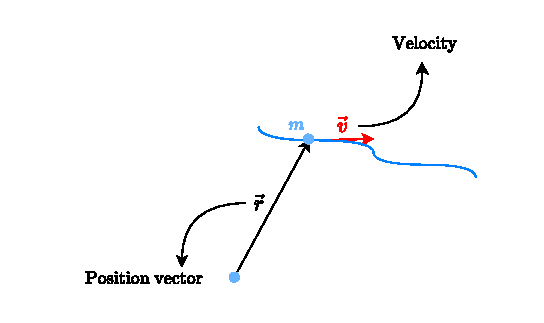
\includegraphics[width=0.6\textwidth]{res/svg/onepartsys.drawio}
    \caption{One particle system}
    \label{fig:image1}
\end{figure}

From that we can derive some quantities:
\begin{itemize}
    \item Linear momentum: \begin{equation}\vec{p}=m\vec{v}\end{equation} While $m$ is constant
    \item Total force applied: \begin{equation}\vec{F}=\dot{\vec{p}}=\dfrac{\mathrm{d} \vec{p}}{\mathrm{d} t}=m\vec{a}\end{equation}The first equality is the original formulation for Newton's second law.\\From this follows the conservation of linear momentum:
    \begin{equation}\vec{F}=0 \iff\dot{\vec{p}}=0 \iff\vec{p}\;\mathrm{is\;constant} \iff\vec{v}\;\mathrm{is\;constant}\end{equation}
    \item Angular momentum:
    \begin{equation}
        \vec{L_{\Omega}} = \left(\vec{r}-\vec{r}_{\Omega}\right) \wedge m\vec{v} = \left(\vec{r}-\vec{r}_{\Omega}\right) \wedge \vec{p}
    \end{equation}
    The angular momentum is a pseudo-vector and it is always calculated with reference to a generic point $\Omega$.
    \begin{figure}[H]
        \centering
        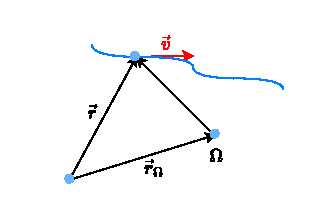
\includegraphics[width=0.6\textwidth]{res/svg/omegareference.drawio}
        \caption{Reference point for angular momentum}
        \label{fig:image2}
    \end{figure}
    Trying to differentiate the angular momentum we get:
    \begin{equation}
        \dfrac{\mathrm{d}\vec{L}_{\Omega}}{\mathrm{d}t} = \dfrac{\mathrm{d}}{\mathrm{d}t}\left(\left(\vec{r}-\vec{r}_{\Omega}\right) \wedge \vec{p}\right) = \dot{\vec{r}}\wedge\vec{p} - \dot{\vec{r}}_{\Omega}\wedge\vec{p} + \left(\vec{r}-\vec{r}_{\Omega}\right) \wedge \vec{F}
    \end{equation}
    \begin{equation}
        \dfrac{\mathrm{d}\vec{L}_{\Omega}}{\mathrm{d}t} = - \vec{v}_{\Omega}\wedge\vec{p} + \vec{\tau}_{\Omega}
    \end{equation}
    If $\Omega$ is at rest we can choose $\Omega = O$ which implies:
    \begin{equation}
        \dfrac{\mathrm{d}\vec{L}_{\Omega}}{\mathrm{d}t} = \vec{\tau}_{\Omega}
    \end{equation}
    From which follows the conservation of angular momentum:
    \begin{equation}
        \vec{\tau}_{\Omega} = 0 \iff\vec{L}_{\Omega}\;\mathrm{is\;constant}
    \end{equation}
    If $\vec{L}_{\Omega}$ is fixed then the trajectory happens on a plane.
    \begin{figure}[H]
        \centering
        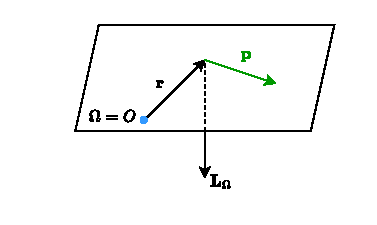
\includegraphics[width=0.6\textwidth]{res/svg/singleplanemotion.drawio}
        \caption{Motion on a single plane}
        \label{fig:image3}
    \end{figure}
\end{itemize}
\section{One particle systems - Work}
The work done by the total force on a particle from point $P_1$ to $P_2$ along a generic path can be visualized as:
\begin{figure}[H]
    \centering
    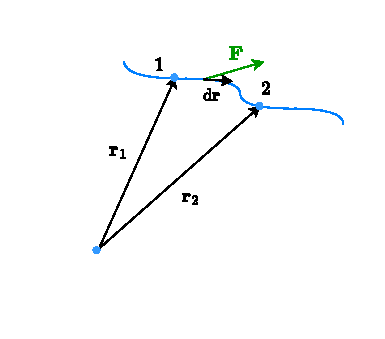
\includegraphics[width=0.5\textwidth]{res/svg/work.drawio}
    \caption{Work of the total force}
    \label{fig:image4}
\end{figure}
and is evaluated as:
\begin{equation}
    W_{12} = \int_{P_1}^{P_2}\vec{F}\cdot\mathrm{d}\vec{r} = \int_{P_1}^{P_2}\dfrac{\mathrm{d}}{\mathrm{d}t}(m\vec{v})\cdot\mathrm{d}\vec{r} = \int_{P_1}^{P_2}\dfrac{\mathrm{d}}{\mathrm{d}t}(m\vec{v})\cdot\vec{v}\mathrm{d}t =
\end{equation}
\begin{equation}
    = m\int_{P_1}^{P_2}\vec{v}\mathrm{d}v = \dfrac{1}{2}mv^2\bigg|_{P_1}^{P_2} = \dfrac{1}{2}mv_2^2 - \dfrac{1}{2}mv_1^2 = T_2 -T_1
\end{equation}
\begin{equation} \label{e:total_work}
    W_{12} = T_2 -T_1
\end{equation}
So the work done by the total force is the difference of the kinetic energy $T$ from point $P_1$ to $P_2$.\\
A force $\vec{f}$ is \textbf{conservative} if its work does not depend on the path:
\begin{equation}
    W_{12} = \int_{P_1,\gamma_1}^{P_2}\vec{f}\cdot\mathrm{d}\vec{r} = \int_{P_1,\gamma_2}^{P_2}\vec{f}\cdot\mathrm{d}\vec{r}\;\;\forall\;\gamma_1, \gamma_2
\end{equation}
\[\Updownarrow \]
\begin{equation}
    \int_{P_1,\gamma_1}^{P_2}\vec{f}\cdot\mathrm{d}\vec{r} - \int_{P_1,\gamma_2}^{P_2}\vec{f}\cdot\mathrm{d}\vec{r} = 0
\end{equation}
\begin{equation}
    \int_{P_1,\gamma_1}^{P_2}\vec{f}\cdot\mathrm{d}\vec{r} + \int_{P_2,\gamma_2}^{P_1}\vec{f}\cdot\mathrm{d}\vec{r} = 0
\end{equation}
\begin{equation}
    \oint\vec{f}\cdot\mathrm{d}\vec{r} = 0
\end{equation}
So if a force is conservative then its circulation is always 0 for any closed path.\\
Also if $\vec{f}$ is conservative we can find a scalar function such that:
\begin{equation}
    \int_{P_1,\gamma}^{P_2}\vec{f}\cdot\mathrm{d}\vec{r} = V_1-V_2
\end{equation}
This function is called the \textbf{potential}:
\begin{equation}
    V_1-V_2 = \int_{P_1}^{P_2}(-\mathrm{d}V) \Rightarrow \vec{f}\cdot\mathrm{d}\vec{r} = -\mathrm{d}V = -\nabla V \cdot \mathrm{d}\vec{r}
\end{equation}
\begin{equation}
    \vec{f} = -\nabla V
\end{equation}
If the total force $\vec{F}$ is conservative (sum of conservative forces) then:
\begin{equation}
    \vec{F} = \bigsum_{i=1}^{N} \vec{f}_i
\end{equation}
\begin{equation}
    W_{12}=\int_{P_1}^{P_2}\vec{f}\cdot\mathrm{d}\vec{r} = \int_{P_1,\gamma}^{P_2}-\nabla V\cdot\mathrm{d}\vec{r}
\end{equation}
Where $V$ is the sum of the potential of the single forces. Now from \eqref{e:total_work}, for conservative forces we get:
\begin{equation} \label{e:mech_energy}
    T_2 - T_1 = V_1 - V_2 \iff T_1 + V_1 = T_2 + V_2\iff E_1 = E_2
\end{equation}
Where $E$ is the total \textbf{mechanical energy} of the system.\\
There can be cases such that:
\begin{equation}
    \vec{F} = -\nabla V \;\;\;\mathrm{but}\;V=V(\vec{r},t)
\end{equation}
then $\vec{F}$ cannot be conservative. We can show this by computing $\mathrm{d}V$:
\begin{equation}
    -\mathrm{d}V = -\left(\dfrac{\partial V}{\partial x}\mathrm{d}x + \dfrac{\partial V}{\partial y}\mathrm{d}y + \dfrac{\partial V}{\partial z}\mathrm{d}z + \dfrac{\partial V}{\partial t}\mathrm{d}t\right) =
\end{equation}
\begin{equation}
    = -\nabla V \cdot\mathrm{d}\vec{r} - \dfrac{\partial V}{\partial t}\mathrm{d}t \neq \vec{F}\cdot\mathrm{d}\vec{r} \Rightarrow \int_{P_1}^{P_2}\vec{F}\cdot\mathrm{d}\vec{r} \neq V_1-V_2
\end{equation}
\section{Multiple particles systems - Definitions}
Similarly to what we established for one particle systems we can define some main characteristics for multiple particles systems:
\begin{itemize}
    \item Mass:\begin{equation}
        M = \bigsum_{i=1}^{N} m_i
    \end{equation}
    \item Linear momentum:\begin{equation}
        \vec{P} = \bigsum_{i=1}^{N} \vec{p}_i
    \end{equation}
    \item Angular momentum (with respect to $\Omega$):\begin{equation}
        \vec{L}_{\Omega} = \bigsum_{i=1}^{N} \left(\left(\vec{r}_i-\vec{r}_{\Omega}\right) \wedge \vec{p}_i\right)
    \end{equation}
    \item Average position (centre of mass): \begin{equation} \label{e:centre_of_mass}
        \vec{R} = \dfrac{\bigsum_{i=1}^{N}m_i\vec{r}_i}{\bigsum_{i=1}^{N}m_i}
    \end{equation}
    From this trivially follows:
    \begin{equation}
        M \vec{R} = \bigsum_{i=1}^{N}m_i\vec{r}_i
    \end{equation}
    \begin{equation}
        \dfrac{\mathrm{d}}{\mathrm{d}t}(M \vec{R}) = \dfrac{\mathrm{d}}{\mathrm{d}t}\left(\bigsum_{i=1}^{N}m_i\vec{r}_i\right)
    \end{equation}
    \begin{equation}
        M \dot{\vec{R}} = \vec{P}
    \end{equation}
    Where $\vec{v}_{CM} = \dot{\vec{R}}$ is the velocity of the centre of mass.
\end{itemize}
\section{Multiple particles systems - Newton's third law}
The total force on a single particle contains two components:
\begin{itemize}
    \item internal forces
    \item external forces
\end{itemize}
\begin{equation}
    \vec{F}_i = \vec{F}_i^{(\mathrm{ext})} + \bigsum_{i\neq j}^{N}\vec{F}_{ji}
\end{equation}
We will restrict to the case where $\vec{F}_{ji} = -\vec{F}_{ij}$. This is called \textbf{weak action law}, since it only requires that the forces are equal and opposite, but it is not necessary that they both lie on the same line.\\
\textbf{Newton's third law} (strong action law) is not always true. Let's show a counterexample.\\
Let there be two charges $q_1,q_2$ with velocity $v_1,v_2$ such that $v_1\perp v_2$. Analysing the moment when particle 2 is on the same line of motion of particle 1, for electrostatic forces we get:
\[||\vec{r}_{12}|| = ||\vec{r}_{21}|| = r\]
\[\vec{r}_{12} = - \vec{r}_{21}\]
\begin{equation}
    \vec{F}_{12} = k\dfrac{q_1q_2}{r^2}\hat{u}_{12} = k\dfrac{q_1q_2 \vec{r}_{12}}{r^3}
\end{equation}
\begin{equation}
    \vec{F}_{21} = k\dfrac{q_1q_2}{r^2}\hat{u}_{21} = k\dfrac{q_1q_2 \vec{r}_{21}}{r^3}
\end{equation}
So these forces satisfy both action laws, but these are not the only forces on the charges. Let's analyze the Lorentz's forces. Particle 1 feels a magnetic field:
\begin{equation}
    \vec{B}_{21} = \dfrac{\muz}{4\pi}\dfrac{q_2\vec{v}_2\wedge\vec{r}_{21}}{r} \neq 0
\end{equation}
Instead particle 2 does not feel any magnetic field since in the chosen moment it is in the direction of motion of the other charge so we have:
\begin{equation}
    \vec{B}_{12} = \dfrac{\muz}{4\pi}\dfrac{q_1\vec{v}_1\wedge\vec{r}_{12}}{r} = 0
\end{equation}
This means that the Lorentz's forces are:
\begin{equation}
    \vec{F}_{21} = q_1\vec{v}_1\wedge\vec{B}_{21} \neq 0
\end{equation}
\begin{equation}
    \vec{F}_{12} = q_2\vec{v}_2\wedge\vec{B}_{12} = 0
\end{equation}
Hence $\vec{F}_{21} \neq \vec{F}_{12}$ and Newton's thrid law is not satisfied.\\
Since we restrict our cases we have:
\begin{equation}
    \vec{F} = \bigsum_{i=1}\vec{F}_i = \bigsum_{i=1}\vec{F}_i^{\;(ext)} + \cancel{\bigsum_{i=1}\bigsum_{j\neq i}\vec{F}_i}\raisebox{14pt}{\scriptsize = 0}
\end{equation}
\begin{equation}
    \vec{F} = \bigsum_{i=1}\vec{F}_i = \bigsum_{i=1}\dfrac{\dd{\vec{p}_i}}{\dd{t}} = \dfrac{\dd{}}{\dd{t}}\bigsum_{i=1}\vec{p}_i = \dfrac{\dd{\vec{P}}}{\dd{t}}
\end{equation}
But also:
\begin{equation}
    \dfrac{\dd{\vec{P}}}{\dd{t}} = \bigsum_{i=1}\vec{F}_i^{\;(ext)}
\end{equation}
So (only if weak action law holds):
\begin{equation}
    \vec{F} = \dfrac{\dd{\vec{P}}}{\dd{t}}
\end{equation}
\section{Multiple particles systems - Angular momentum}
Starting from the definition:
\begin{equation}
    \vec{L}_{\Omega} = \bigsum_{i}\brackets{\vec{r}_i-\vec{r}_{\Omega}}\wedge\vec{p}_i
\end{equation}
\begin{equation}
    \dfrac{\dd{\vec{L}_{\Omega}}}{\dd{t}} = \bigsum_{i}\dfrac{\dd{}}{\dd{t}}\brackets{\vec{r}_i-\vec{r}_{\Omega}}\wedge\vec{p}_i + \bigsum_{i}\brackets{\vec{r}_i-\vec{r}_{\Omega}}\wedge\dfrac{\dd{\vec{p}_i}}{\dd{t}} =
\end{equation}
\begin{equation}
    = \crossout{\bigsum_{i}\vec{v}_i\wedge\vec{p}_i}-\bigsum_{i}\vec{v}_{\Omega}\wedge\vec{p}_i + \bigsum_{i}\brackets{\vec{r}_i-\vec{r}_{\Omega}}\wedge\vec{F}_i =
\end{equation}
\begin{equation}
    = -\vec{v}_{\Omega}\wedge\bigsum_{i}\vec{p}_i + \bigsum_{i}\brackets{\vec{r}_i-\vec{r}_{\Omega}}\wedge\vec{F}_i = -\vec{v}_{\Omega}\wedge\vec{P} + \bigsum_{i}\brackets{\vec{r}_i-\vec{r}_{\Omega}}\wedge\vec{F}_i
\end{equation}
We can simplify the first term since $\vec{v}_i \parallel \vec{p}_i$ and we can also see that the last term is the \textbf{total torque} $\vec{\tau}_{\Omega}$, which is the result of both the internal and external forces.
\begin{equation} \label{e:first_angular_expression}
    \dfrac{\dd{\vec{L}_{\Omega}}}{\dd{t}} = -\vec{v}_{\Omega}\wedge\vec{P} + \vec{\tau}_{\Omega}
\end{equation}
If we restrict to the strong action law we get:
\begin{equation}
    \vec{\tau}_{\Omega} = \bigsum_{i}\brackets{\vec{r}_i-\vec{r}_{\Omega}}\wedge\vec{F}_i = \bigsum_{i}\brackets{\vec{r}_i-\vec{r}_{\Omega}}\wedge\brackets{\vec{F}_i^{\;(ext)}+ \bigsum_{i\neq j}\vec{F}_{ji}} =
\end{equation}
\begin{equation}
    = \bigsum_{i}\brackets{\vec{r}_i-\vec{r}_{\Omega}}\wedge\vec{F}_i^{\;(ext)} + \crossout{\bigsum_{i}\brackets{\brackets{\vec{r}_i-\vec{r}_{\Omega}}\wedge\bigsum_{i\neq j}\vec{F}_{ji}}} = \vec{\tau}^{\;(ext)}
\end{equation}
We can cross out the second term since the sum only has terms such as:
\begin{equation}
    \vec{r}_i\wedge\vec{F}_{ji} + \vec{r}_j\wedge\vec{F}_{ij}-\crossout{{\vec{r}_{\Omega}\wedge\vec{F}_{ij}+\vec{r}_{\Omega}\wedge\vec{F}_{ji}}}
\end{equation}
This first simplification is a trivial consequence of weak action law. In order to simplify the other term we can realize that if strong action law holds then both $\vec{F}_{ij}$ and $\vec{F}_{ji}$ lie on the line of $\vec{r}_i-\vec{r}_j$ and have opposite directions.
So we get:
\begin{equation}
    \bigsum_{i}\brackets{\brackets{\vec{r}_i-\vec{r}_{\Omega}}\wedge\bigsum_{i\neq j}\vec{F}_{ji}} = 0
\end{equation}
Going back to \eqref{e:first_angular_expression} we get:
\begin{equation}
    \dfrac{\dd{\vec{L}_{\Omega}}}{\dd{t}} = -\vec{v}_{\Omega}\wedge\vec{P} + \vec{\tau}^{\;(ext)}
\end{equation}
The first term can be 0 if:
\begin{itemize}
    \item $\Omega$ is at rest
    \item $\Omega$ is a point such that $\vec{v}_{\Omega} \parallel \vec{P}$ (for example the centre of mass)
    \item $\vec{P}=0$
\end{itemize}
So in the case of $\Omega = \mathrm{CM}$ we have:
\begin{equation} \label{e:first_cardinal}
    \dfrac{\dd{\vec{L}_{\Omega}}}{\dd{t}} = \vec{\tau}_{\Omega}
\end{equation}
Then:
\begin{equation}
    \vec{L}_{\Omega}\;\mathrm{is\;constant} \iff \vec{\tau}_{\Omega}^{\;(ext)}=0
\end{equation}
The centre of mass also satisfies:
\begin{equation}
    \vec{P} = M\dvec{R}
\end{equation}
as if the mass was all concentrated in the CM. But for angular momentum:
\begin{equation}
    \vec{L}_{\Omega} \neq (\vec{R}-\vec{r}_{\Omega})\wedge\vec{P}
\end{equation}
instead this is true:
\begin{equation}
    \vec{L}_{\Omega} = (\vec{R}-\vec{r}_{\Omega})\wedge\vec{P} + \vec{L}'_{CM}
\end{equation}
Where $\vec{L}'_{CM}$ is the total angular momentum evaluated in the frame of reference of the centre of mass.\\
From this we can state \textbf{Konig's theorem}:
\begin{equation}
    T = \dfrac{1}{2}\bigsum_i m_i v_i^2 = T_{CM} + T' = \dfrac{1}{2}M v_{CM}^2 + T'
\end{equation}
Where $T'$ is the kinetic energy associated to the motion with respect to the centre of mass.\\
Now we can analyze the work of the system of particles:
\begin{equation}
    W_{12} = \bigsum_i\int_{1}^{2}\vec{F}_i = \int_{1}^{2}\bigsum_i\vec{F}_i = \int_{1}^{2}\bigsum_i\brackets{\vec{F}_i^{\;(ext)} + \bigsum_{j\neq i}\vec{F}_{ji}}\cdot \dd{\vec{r}_i} =
\end{equation}
\begin{equation}
    = \int_{1}^{2}\brackets{\bigsum_i\vec{F}_i^{\;(ext)} + \bigsum_i\bigsum_{j\neq i}\vec{F}_{ji}}\cdot \dd{\vec{r}_i}
\end{equation}
The term $\bigsum_i\bigsum_{j\neq i}\vec{F}_{ji}\cdot \dd{\vec{r}_i}$ is not necessarily 0, but it is 0 in the case of rigid bodies.\\
If external forces are conservative:
\begin{equation}
    \vec{F}_i^{\;(ext)} = -\nabla_i V_i
\end{equation}
The gradient with respect to i is $\nabla_i = \brackets{\partial_{x_i}, \partial_{y_i}, \partial_{z_i}}$. So the work of external forces is just:
\begin{equation}
    W_{12}^{\;(ext)} = \int_{1}^{2}\bigsum_i\brackets{\vec{F}_i\cdot\dd{\vec{r}_i}} = -\bigsum_i\int_{1}^{2}\nabla_i V_i\cdot\dd{\vec{r}_i} =
\end{equation}
\begin{equation}
    = -\bigsum_i\int_{1}^{2}\dd{V_i} = -\bigsum_i V_i\bigg|_1^2
\end{equation}
Now defining $V^{\;(ext)} = \bigsum_i V_i$ we get:
\begin{equation}
    W_{12}^{\;(ext)} = V^{\;(ext)}_1 - V^{\;(ext)}_2
\end{equation}
Now we can see that if forces obey both the strong and the weak action law both $\vec{F}_{ji}$ and $\vec{F}_{ij}$ lie on the line of $\vec{r}_{ij} = \vec{r}_i-\vec{r}_j$ as shown in this example:
\begin{figure}[H]
    \centering
    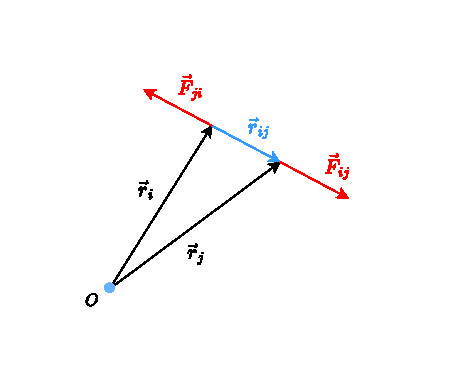
\includegraphics[width=0.5\textwidth]{res/svg/forcesstronglaw.drawio}
    \caption{Forces with strong action law}
    \label{fig:image5}
\end{figure}
Now assuming the forces are conservative we can express them as:
\begin{itemize}
    \item $\vec{F}_{ij}= -\nabla_{j}V_{ij}$
    \item $\vec{F}_{ji}= -\nabla_{i}V_{ji}$
\end{itemize}
But in this case $V_{ij}=V_{ji}$ so, from the strong action law we get:
\begin{equation}
    -\nabla_iV_{ij}=\nabla_jV_{ij}
\end{equation}
We can also express both forces with a unique gradient:
\begin{equation}
    \nabla_{ij} = \brackets{\dfrac{\partial}{\partial(x_j-x_i)},\dfrac{\partial}{\partial(y_j-y_i)},\dfrac{\partial}{\partial(z_j-z_i)}}
\end{equation}
For the first force we have:
\begin{equation}
    \vec{F}_{ji}=-\nabla_iV_{ij}=-\brackets{\dfrac{\partial V_i}{\partial x_i },\dfrac{\partial V_i}{\partial y_i },\dfrac{\partial V_i}{\partial z_i }} =
\end{equation}
\begin{equation}
    =-\brackets{\dfrac{\partial V_i}{\partial x_i}\dfrac{\partial r_{ij}}{\partial r_{ij}},\dfrac{\partial V_i}{\partial y_i }\dfrac{\partial r_{ij}}{\partial r_{ij}},\dfrac{\partial V_i}{\partial z_i }\dfrac{\partial r_{ij}}{\partial r_{ij}}}
\end{equation}
The partial derivatives of $r_{ij}$ are in the form of:
\begin{equation}
    \dfrac{\partial r_{ij}}{\partial x_i} = \dfrac{\partial }{\partial x_i}\sqrt{(x_j-x_i)^2 + (y_j-y_i)^2+ (z_j-z_i)^2} =
\end{equation}
\begin{equation}
    = \dfrac{(x_j-x_i)}{\sqrt{(x_j-x_i)^2 + (y_j-y_i)^2+ (z_j-z_i)^2}}
\end{equation}
So the sum becomes:
\begin{equation}
    \dfrac{(x_j-x_i)+(y_j-y_i)+(z_j-z_i)}{\sqrt{(x_j-x_i)^2 + (y_j-y_i)^2+ (z_j-z_i)^2}} = \dfrac{\vec{r}_{ij}}{||\vec{r}_{ij}||} = \hat{u}_{ij}
\end{equation}
And so we get that the force is:
\begin{equation}
    \vec{F}_{ji}= \dfrac{\partial V}{\partial r_{ij}}\hat{u}_{ij} = \nabla_{ij}V
\end{equation}
Doing the same for $\vec{F}_{ij}$ we get:
\begin{equation}
    \vec{F}_{ij}= -\dfrac{\partial V}{\partial r_{ij}}\hat{u}_{ij}= -\nabla_{ij}V
\end{equation}
If the internal forces are conservative $V$ must depend only on the magnitude of the distance ($r_{ij}$). Hence:
\begin{equation}
    W^{(int)}=\dfrac{1}{2}\int_{1}^{2}\bigsum_i\bigsum_j\vec{F}_{ji}\cdot\dd{\vec{r}_i}
\end{equation}
The double summation contains terms such as:
\begin{equation}
    \vec{F}_{ji}\cdot\dd{\vec{r}_i} + \vec{F}_{ij}\cdot\dd{\vec{r}_j} = \nabla_{ij}V\cdot\dd{\vec{r}_i} + -\nabla_{ij}V\cdot\dd{\vec{r}_j} = -\nabla_{ij}V\cdot\brackets{\dd{\vec{r}_i}-\dd{\vec{r}_j}}
\end{equation}
Now naming the differential $\dd{\vec{r}_{ij}}=\dd{\vec{r}_i}-\dd{\vec{r}_j}$ and recalling that $-\nabla_{ij}V\cdot\dd{\vec{r}_{ij}} = -\dd{V_{ij}}$ we get:
\begin{equation}
    W^{(int)}=-\dfrac{1}{2}\int_{1}^{2}\bigsum_i\bigsum_j\dd{V_{ij}} = -\dfrac{1}{2}\bigsum_i\bigsum_j V_{ij}\bigg|_{1}^{2}
\end{equation}
So the total work is:
\begin{equation}
    W = W^{\;(ext)}+W^{(int)}= -\bigsum_i V_i\bigg|_{1}^{2} -\dfrac{1}{2}\bigsum_i\bigsum_j V_{ij}\bigg|_{1}^{2}
\end{equation}
Defining $V=-\bigsum_i V_i -\dfrac{1}{2}\bigsum_i\bigsum_j V_{ij}$ the total work is:
\begin{equation}
    W = V_1-V_2
\end{equation}
But the total work is also:
\begin{equation}
    W = \int_{1}^{2}\bigsum_i \vec{F}_i \cdot \dd{r_i}= \bigsum_i \int_{1}^{2} \vec{F}_i \cdot \dd{r_i} = T_2 - T_1
\end{equation}
So, for conservative systems we get:
\begin{equation}
    T_2 - T_1 = V_1 - V_2 \iff T_2 + V_2 = T_1 + V_1 \iff E_2 = E_1
\end{equation}
Which is the mathematical expression for the conservation of mechanical energy.

\chapter{Constraints}
\section{Definitions}
Any physical system has constraints which limit the motion of parts of the system. They act through forces (forces of constraint). Those forces are unknown and must be obtained through Newton's laws from the effects on other forces.\\
\subsection{\textbf{Ex.} Normal forces:}
\begin{figure}[H]
    \centering
    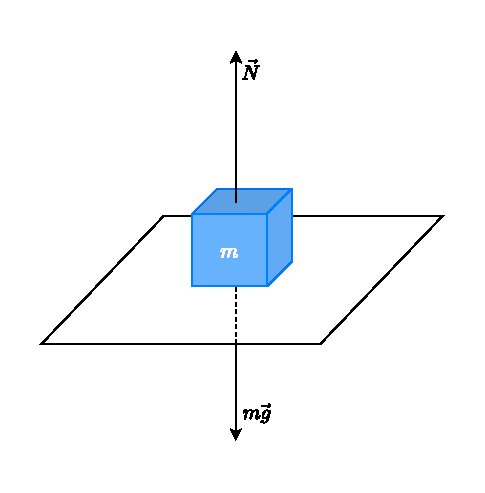
\includegraphics[width=0.5\linewidth]{res/svg/normalforce.drawio}
    \caption{Normal force on a plane}
    \label{fig:image6}
\end{figure}
Let's look deeper with another example. Imagine taking two masses $m_1$ and $m_2$ attached with an inextensible rope through an ideal pulley (massless and frictionless). Also consider the plane frictionless, we get this type of situation:
\begin{figure}[H]
    \centering
    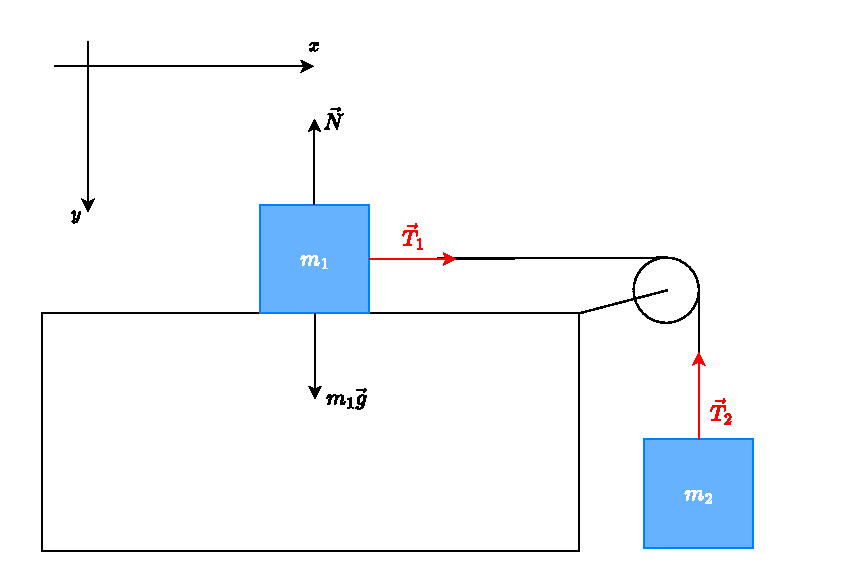
\includegraphics[width=0.6\linewidth]{res/svg/idealpulley.drawio}
    \caption{Normal force on a plane}
    \label{fig:image7}
\end{figure}
The ideal pulley gives us the information that $I\alpha = 0 \Rightarrow T_1 = T_2$. We also know that:
\[a_1 = a_2\]
This is the effect of the inextensible rope which is a \textbf{constraint} for the system. Solving Newton's equations leads to:
\begin{equation}
    \centering
\begin{cases}
T_1=T_2=m_1a \\[8pt]
m_2g -T =m_2a \\[8pt]
\end{cases} \Rightarrow a = \dfrac{m_2}{m_1+m_2}g
\end{equation}
\begin{definition}{Holonomic constraint}
  A constraint is said to be holonomic if it can be expressed as a function:
  \begin{equation}
    f(\vec{r}_1,\vec{r}_2, \,\dots\, ,\vec{r}_n,t) = 0
  \end{equation}
\end{definition}
For the inextensible rope the constraint can be expressed as $\dd{x}=\dd{y}$, but if we choose an appropriate frame of reference the condition can also simply be $x=y$, so the rope is a holonomic constraint such that:
\begin{equation}
    f(x,y)=0 \Rightarrow x-y=0
\end{equation}
If a constraint can be expressed as a function of the velocities it is said to be \textbf{semi-holonomic} and has a form such as:
\begin{equation}
    f(\dvec{r}_1,\dvec{r}_2, \,\dots\, ,\dvec{r}_n,t) = 0
\end{equation}
There are two main types of holonomic constraints:
\begin{itemize}
    \item \textbf{scleronomic} if it \underline{does not} depend on time explicitly \[f(\vec{r}_1,\vec{r}_2, \,\dots\, ,\vec{r}_n) = 0\]
    \item \textbf{rheonomic} if it \underline{does} depend on time explicitly \[f(\vec{r}_1,\vec{r}_2, \,\dots\, ,\vec{r}_n,t) = 0\]
\end{itemize}
A constraint allows us to express any coordinate as a function of the others, so, if we have $N$ particle we should have $3N$ coordinates, but if we have $K$ constraints the actual number of independent coordinates is:
\begin{equation}
    n = 3N-K = \text{dof (degrees of freedom)}
\end{equation}
\section{Virtual displacement}
\begin{definition}{Virtual displacement}
  A virtual displacement is an infinitesimal change in the configuration of the system that results in a change in the particle position compatible with the forces of constraint of the system \underline{at a given time}.
\end{definition}
To explain the difference between a virtual displacement and an actual displacement we can analyze the displacement of a moving object on an inclined plane with the angle changing over time:
\begin{figure}[H]
  \centering
  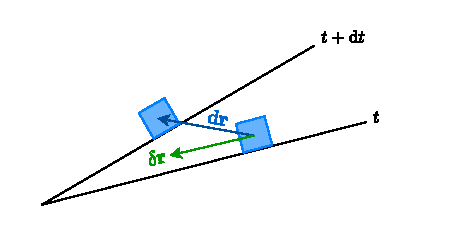
\includegraphics[width=0.5\linewidth]{res/svg/virtualdisplacement.drawio}
  \caption{Displacement and virtual displacement}
  \label{fig:image8}
\end{figure}
Where:
\begin{itemize}
    \item $\delta \vec{r}$ is the virtual displacement
    \item $\dd{\vec{r}}$ is the actual displacement
\end{itemize}
Now consider a system of particles at equilibrium so that:
\begin{equation}
    \vec{F}_i = 0\;\forall i
\end{equation}
The total force is composed of two separated parts:
\begin{itemize}
    \item Applied forces $\vec{F}^{(a)}_i$
    \item Constraint forces $\vec{f}_i$
\end{itemize}
At equilibrium we get:
\begin{equation}
    \begin{split}
      &\bigsum_i \vec{F}_i \cdot \delta \vec{r}_i = 0 \\[8pt]
      &\bigsum_i \brackets{\vec{F}^{(a)}_i + \vec{f}_i} \cdot \delta \vec{r}_i = \bigsum_i \vec{F}^{(a)}_i \cdot \delta \vec{r}_i + \bigsum_i \vec{f}_i \cdot \delta \vec{r}_i = 0
    \end{split}
\end{equation}
Now we consider only system with zero total virtual work, and we get:
\begin{equation}
    \begin{split}
      &\bigsum_i \vec{F}^{(a)}_i \cdot \delta \vec{r}_i + \cancel{\bigsum_i \vec{f}_i \cdot \delta \vec{r}_i} = 0 \\[8pt]
      &\bigsum_i \vec{F}^{(a)}_i \cdot \delta \vec{r}_i = 0
    \end{split}
\end{equation}
The last equation represents the condition of equilibrium for a system such that $\bigsum_i \vec{f}_i \cdot \delta \vec{r}_i = 0$ and is called \textbf{principle of virtual work}.
If the system \underline{is not} at equilibrium then we have:
\begin{equation}
    \vec{F}_i = \dvec{p}_i \Rightarrow \vec{F}_i - \dvec{p}_i = 0
\end{equation}
From which follows:
\begin{equation}
    \bigsum_i \brackets{\vec{F}_i - \dvec{p}_i} \cdot \delta \vec{r}_i = \bigsum_i \brackets{\vec{F}^{(a)}_i + \vec{f}_i - \dvec{p}_i} \cdot \delta \vec{r}_i = 0
\end{equation}
Now if the total virtual work of constraints is 0:
\begin{equation}
    \bigsum_i \brackets{\vec{F}^{(a)}_i - \dvec{p}_i} \cdot \delta \vec{r}_i + \cancel{\bigsum_i \vec{f}_i \cdot \delta \vec{r}_i} = 0
\end{equation}
And we get the so called \textbf{D'Alembert's principle}:
\begin{equation}  \label{D'Alembert_principle}
    \boxed{\bigsum_i \brackets{\vec{F}^{(a)}_i - \dvec{p}_i} \cdot \delta \vec{r}_i = 0}
\end{equation}
Now a problem arises. Since the $\delta \vec{r}_i$ are not independent in these coordinates we need to find a new set of coordinates that makes us able to make all the terms in the sum independent so we can establish that every single term is independently zero.
Those coordinates are called \textbf{generalized coordinates}.\\
Let us now consider only holonomic constraints so we have:
\begin{itemize}
    \item $N$ particles $\Rightarrow$ $3N$ coordinates
    \item $K$ constraints
\end{itemize}
So we actually have $n = 3N-K$ independent coordinates as we stated while talking about constraints in general. So we define the general coordinates:
\begin{equation}
    q_{\alpha}\;\forall\;\alpha = 1, \,\dots\, ,n
\end{equation}
As we stated all the original coordinates must only depend on the $q_{\alpha}$'s and (eventually) on time.
\begin{equation} \label{equations_of_transformation}
    \begin{cases}
        \vec{r}_1 = \vec{r}_1\brackets{q_1, \,\dots\, ,q_n,t}\\[8pt]
        \vec{r}_2 = \vec{r}_2\brackets{q_1, \,\dots\, ,q_n,t}\\[8pt]
         \,\dots\,  \\[8pt]
        \vec{r}_N = \vec{r}_N\brackets{q_1, \,\dots\, ,q_n,t}
    \end{cases}
\end{equation}
These are called the \textbf{equations of transformation}, and they have some properties:
\begin{itemize}
    \item explicitly contain the constraints
    \item can depend on time or not
    \item $q_{\alpha}$'s may not be lengths
    \item $q_{\alpha}$'s may not be grouped in vectors
    \item $q_{\alpha}$'s are scalars
\end{itemize}
An example of the use of generalized coordinates is the use of polar coordinates for the analysis of the pendulum system. In that case there are only 2 coordinates, but there is a constraint on the distance between the mass and the pole of the rotation, so we only have one independent coordinate:
\[q=\theta\]
Obviously it is possible to express general coordinates in terms of regular coordinates:
\begin{equation} \label{inverse_equations_of_transformation}
    \begin{cases}
        q_1 = q_1\brackets{\vec{r}_1, \,\dots\, ,\vec{r}_N,t}\\[8pt]
        q_2 = q_2\brackets{\vec{r}_1, \,\dots\, ,\vec{r}_N,t}\\[8pt]
         \,\dots\,  \\[8pt]
        q_n = q_n\brackets{\vec{r}_1, \,\dots\, ,\vec{r}_N,t}
    \end{cases}
\end{equation}

\chapter{Lagrange and Euler-Lagrange mechanics}
In this section we will discuss the main possible formulations of classical mechanics and their derivations. We also want to note that all the formulations are derived from Newton's equations and so they are completely equivalent to them if the conditions for their validity are satisfied.
\section{Lagrange equations}
Going back to \dalembertref, expressing in generalized coordinates:
\begin{equation}
    \bigsum_i \brackets{\vec{F}^{\cancel{(a)}}_i - \dvec{p}_i} \cdot \delta \vec{r}_i = 0
\end{equation}
We drop the (a) term for an easier notation, from now on we will write $\vec{F}_i$ knowing that we are indicating the applied force.
\begin{equation}
    \delta \vec{r}_i = \bigsum_{\alpha} \dfrac{\partial \vec{r}_i}{\partial q_{\alpha}} \delta q_{\alpha} + \cancel{\dfrac{\partial \vec{r}_i}{\partial t} \dd{t}}
\end{equation}
The partial derivative over time is zero since we are considering a fixed moment in time. The force term in \dalembertref\;becomes:
\begin{equation}
    \bigsum_i \vec{F}_i \cdot \bigsum_{\alpha} \dfrac{\partial \vec{r}_i}{\partial q_{\alpha}} \delta q_{\alpha} = \bigsum_{\alpha}\underbrace{\bigsum_{i} \vec{F}_i \cdot \dfrac{\partial \vec{r}_i}{\partial q_{\alpha}}}_{Q_{\alpha}} \delta q_{\alpha} = \bigsum_{\alpha}Q_{\alpha}\delta q_{\alpha}
\end{equation}
The terms $Q_{\alpha}$ are called \textbf{generalized components of the forces}.
Now let's consider the expression $\bigsum_i \dvec{p}_i \cdot \delta \vec{r}_i$. We know that:
\begin{itemize}
    \item $\dvec{p}_i = \dv{}{t}\brackets{m_i\vec{v}_i}$
    \item $\delta \vec{r}_i = \bigsum_{\alpha} \dfrac{\partial \vec{r}_i}{\partial q_{\alpha}}\delta q_{\alpha}$
\end{itemize}
Now, from the product rule:
\begin{equation} \label{e:total_deriv}
    \dv{}{t}\brackets{m_i\vec{v}_i \cdot \dfrac{\partial \vec{r}_i}{\partial q_{\alpha}}} = \dv{}{t}\brackets{m_i\vec{v}_i}\cdot \dfrac{\partial \vec{r}_i}{\partial q_{\alpha}} + m_i\vec{v}_i \cdot \dv{}{t}\brackets{\dfrac{\partial \vec{r}_i}{\partial q_{\alpha}}}
\end{equation}
From the last term we get:
\begin{equation} \label{e:funny_derivative_p1}
    \begin{split}
      m_i\vec{v}_i \cdot \dv{}{t}\brackets{\dfrac{\partial \vec{r}_i}{\partial q_{\alpha}}} &= m_i\vec{v}_i \cdot \bigsum_{\beta} \dfrac{\partial}{\partial \dot{q}_{\beta} }\brackets{\dfrac{\partial \vec{r}_i}{\partial q_{\alpha}}} q_{\beta} + \dfrac{\partial}{\partial t}\brackets{\dfrac{\partial \vec{r}_i}{\partial q_{\alpha}}} = \\[8pt]
      &= m_i\vec{v}_i \cdot \dfrac{\partial}{\partial q_{\alpha} }\underbrace{\left[\bigsum_{\beta} \dfrac{\partial \vec{r}_i}{\partial q_{\beta}} \dot{q}_{\beta} + \dfrac{\partial \vec{r}_i}{\partial t}\right]}_{\dvec{v}_i} = m_i\vec{v}_i \cdot \dfrac{\partial \vec{v}_i}{\partial q_{\alpha}}
    \end{split}
\end{equation}
We now aim to prove that the partial derivative with respect to alpha in the first term in \eqref{e:total_deriv} is:
\begin{equation}
    \dfrac{\partial \vec{r}_i}{\partial q_{\alpha}} = \dfrac{\partial \vec{v}_i}{\partial \dot{q}_{\alpha}}
\end{equation}
Deriving what we got in \eqref{e:funny_derivative_p1} we get:
\begin{equation}
    \begin{split}
      \dfrac{\partial \vec{v}_i}{\partial \dot{q}_{\alpha}} &= \dfrac{\partial }{\partial \dot{q}_{\alpha}} \brackets{\bigsum_{\beta}\dfrac{\partial \vec{r}_i}{\partial q_{\beta}} \dot{q}_{\beta} + \dfrac{\partial \vec{r}_i}{\partial t}} = \\[8pt]
      &= \bigsum_{\beta}\dfrac{\partial \vec{r}_i}{\partial q_{\beta}} \underbrace{\dfrac{\partial \dot{q}_{\beta}}{\partial \dot{q}_{\alpha}}}_{\delta_{\alpha \beta}}  + \cancel{\dfrac{\partial }{\partial \dot{q}_{\alpha}}\brackets{\dfrac{\partial \vec{r}_i}{\partial t}}} = \dfrac{\partial \vec{r}_i}{\partial q_{\alpha}}
    \end{split}
\end{equation}
Again, the first term of \eqref{e:total_deriv} can be rewritten as:
\begin{equation}
    \bigsum_i \dv{}{t}\brackets{m_i\vec{v}_i \cdot \dfrac{\partial \vec{r}_i}{\partial q_{\alpha}}} = \bigsum_i\dv{}{t}\brackets{m_i\vec{v}_i \cdot \dfrac{\partial \vec{v}_i}{\partial \dot{q}_{\alpha}}} = \dv{}{t}\left[\dfrac{\partial }{\partial \dot{q}_{\alpha}} \underbrace{\bigsum_i \brackets{\dfrac{1}{2}m_i \vec{v}_i \cdot \vec{v}_i}}_{T}\right]
\end{equation}
Similarly the last term in \eqref{e:total_deriv} is:
\begin{equation}
    \bigsum_im_i\vec{v}_i \cdot \dfrac{\partial \vec{v}_i}{\partial q_{\alpha}} = \dfrac{\partial }{\partial \dot{q}_{\alpha}} \underbrace{\bigsum_i \brackets{\dfrac{1}{2}m_i \vec{v}_i \cdot \vec{v}_i}}_{T}
\end{equation}
So we get:
\begin{equation}
    \bigsum_i \dv{}{t}\brackets{m_i\vec{v}_i}\cdot \dfrac{\partial \vec{r}_i}{\partial q_{\alpha}} = \dv{}{t}\dfrac{\partial T}{\partial \dot{q}_{\alpha}} - \dfrac{\partial T}{\partial q_{\alpha}}
\end{equation}
Going back to \dalembertref\;we get:
\begin{equation}
    \begin{split}
      \bigsum_i \brackets{\vec{F}_i - \dvec{p}_i} \cdot \delta \vec{r}_i &= \bigsum_{\alpha}Q_{\alpha}\delta q_{\alpha} - \bigsum_i \dv{}{t}\brackets{m_i\vec{v}_i} \cdot \bigsum_{\alpha}\dfrac{\partial \vec{r}_i}{\partial q_{\alpha}}\delta q_{\alpha} = \\[8pt]
      &= \bigsum_{\alpha}Q_{\alpha}\delta q_{\alpha} - \bigsum_{\alpha}\bigsum_i \dv{}{t}\brackets{m_i\vec{v}_i} \cdot \dfrac{\partial \vec{r}_i}{\partial q_{\alpha}}\delta q_{\alpha} = \\[8pt]
      &= \bigsum_{\alpha}Q_{\alpha}\delta q_{\alpha} - \bigsum_{\alpha}\brackets{\dv{}{t}\dfrac{\partial T}{\partial \dot{q}_{\alpha}} - \dfrac{\partial T}{\partial q_{\alpha}}}\delta q_{\alpha} = 0
    \end{split}
\end{equation}
All the terms are independent by construction so we get a set of equations which are called \textbf{Lagrange equations} $\heartsuit$:
\begin{equation} \label{Lagrange_equations}
    \boxed{\dv{}{t}\dfrac{\partial T}{\partial \dot{q}_{\alpha}} - \dfrac{\partial T}{\partial q_{\alpha}} = Q_{\alpha}}
\end{equation}
which must be satisfied $\forall \alpha$s.
Here are some basic properties of \lagrangeref :
\begin{itemize}
    \item There is a minimum of $n$ equations to solve
    \item They are $2^\circ$ order differential equations, this means that for every equation we need 2 initial conditions
    \item There is a total of $2n$ total initial conditions
\end{itemize}
\section{Euler-Lagrange equations}
From \lagrangeref\;it is easy to derive another formulation. Suppose that every force is expressed through a potential:
\begin{equation}
    \vec{F}_i = -\nabla_i V
\end{equation}
Since $V$ (the total potential) must be a function of only the coordinates $V = V(\vec{r}_i)$ we get that:
\begin{equation}
    Q_{\alpha} = \bigsum_i \vec{F}_i \cdot \dfrac{\partial \vec{r}_i}{\partial q_{\alpha}} = - \bigsum_i \nabla_i V \cdot \dfrac{\partial \vec{r}_i}{\partial q_{\alpha}} = -\partial{V}{q_{\alpha}}
\end{equation}
Rewriting \lagrangeref\;we get:
\begin{equation}
    \dv{}{t}\dfrac{\partial T}{\partial \dot{q}_{\alpha}} - \dfrac{\partial T}{\partial q_{\alpha}} + \partial{V}{q_{\alpha}} = 0
\end{equation}
If the potential does not depend on the generalized velocities we can subtract its derivative with respect to $\dot{q}_{\alpha}$, which will just be 0:
\begin{equation}
    \dv{}{t}\dfrac{\partial }{\partial \dot{q}_{\alpha}}[\underbrace{T-V}_\lagr ] - \dfrac{\partial}{\partial q_{\alpha}}[\underbrace{T-V}_\lagr ] = 0
\end{equation}
We define the Lagrange function or \textbf{Lagrangian} as:
\begin{equation}
    \lagr  = T - V
\end{equation}
Finally we can write the \textbf{Euler-Lagrange equations}:
\begin{equation} \label{Euler_Lagrange_equations}
    \boxed{\dv{}{t}\pdv{\lagr}{\dot{q}_{\alpha}} = \pdv{\lagr}{q_{\alpha}}}
\end{equation}
Here are some basic properties of \eleref :
\begin{itemize}
    \item They are $2^\circ$ order differential equations
    \item There is a total of $2n$ total initial conditions
    \item $\lagr = \lagr(q_{\alpha},\dot{q}_{\alpha},t)$ which means we have $2n+1$ variables
    \item $[\lagr] = \mathrm{J}$ but the Lagrangian is not the mechanical energy, it is just a mathematical tool
    \item If $\lagr$ is a Lagrangian of the system then $\tilde{\lagr} = \lagr + \mathrm{constant}$ is still Lagrangian
    \item If $\lagr$ is a Lagrangian of the system and $F\in \mathcal{C}^1$ is an arbitrary function of \underline{coordinates and time} then $\tilde{\lagr} = \lagr + \partial_t F$ is a Lagrangian
\end{itemize}
If we have two system, let's call them $A$ and $B$ then the Lagrangian of the total system $AB$ in general \underline{is not}:
\begin{equation}
    \lagr_{AB} = T_A + T_B - V_A - V_B - \underbrace{V_{AB}}_{\text{interaction term}}\neq \lagr_A + \lagr_B
\end{equation}
but if the systems interact weakly then:
\begin{equation}
    \lagr_{AB} \approx \lagr_A + \lagr_B
\end{equation}
If the potential $V$ \underline{does not} depend on time explicitly then the system is conservative:
\begin{equation}
    \begin{split}
      \delta W &= \bigsum_i \vec{F}_i \delta \vec{r}_i = \bigsum_i \vec{F}_i \bigsum_{\alpha}\dfrac{\partial \vec{r}_i}{\partial q_{\alpha}}\delta q_{\alpha} = \bigsum_{\alpha} Q_{\alpha}\delta q_{\alpha} = \\[8pt]
      &= -\bigsum_{\alpha} \partial{V}{q_{\alpha}}\delta q_{\alpha} = -\dd{V}
    \end{split}
\end{equation}
Instead if $V$ \underline{depends} on time explicitly we have that:
\begin{equation}
    \dd{V} = \bigsum_{\alpha} \partial{V}{q_{\alpha}}\delta q_{\alpha} + \dfrac{\partial V}{\partial t}\dd{t}
\end{equation}
The extra term appearing in $\dd{V}$ is not present in the expression for work, meaning that:
\begin{equation}
    W_{12} \neq -\int_{1}^{2}\dd{V} = V_1 - V_2
\end{equation}
so the system is not conservative.\\
In some cases (ex. Lorentz force) the force does not come from a "real" potential, we can then rewrite \eleref\;for a function called \textbf{generalized potential} $\mu$ such that:
\begin{equation}
    Q_{\alpha} = -\dfrac{\partial \mu}{\partial q_{\alpha}} +\dv{}{t}\dfrac{\partial \mu}{\partial \dot{q}_{\alpha}}
\end{equation}
Indeed, from \lagrangeref\;we get:
\begin{equation}
    \begin{split}
      \dv{}{t}\dfrac{\partial T}{\partial \dot{q}_{\alpha}} - \dfrac{\partial T}{\partial q_{\alpha}} &= -\dfrac{\partial \mu}{\partial q_{\alpha}} +\dv{}{t}\dfrac{\partial \mu}{\partial \dot{q}_{\alpha}} \\[8pt]
      \dv{}{t}\dfrac{\partial }{\partial \dot{q}_{\alpha}}[\underbrace{T-\mu}_{\lagr}] &- \dfrac{\partial}{\partial q_{\alpha}}[\underbrace{T-\mu}_{\lagr}] = 0 \\[8pt]
      \dv{}{t}\pdv{\lagr}{\dot{q}_{\alpha}} &= \pdv{\lagr}{q_{\alpha}}
    \end{split}
\end{equation}
where we defined a generalized Lagrangian $\lagr = T-\mu$. These are called \textbf{generalized Euler-Lagrange equations}.
\section{Derivation of Euler-Lagrange equations from Hamilton's principle}
A \textbf{monogenic system} is any system in which all the forces can be expressed through a (generalized) potential which depends on $q_{\alpha}$, $\dot{q}_{\alpha}$ and $t$.
\begin{definition}{Configuration space}
  Configuration space is the set of all the $q_{\alpha}$. It completely describes the position of each particle of the system at a givent time which, indeed, is the configuration of the system itself
\end{definition}
We can imagine the configuration space as an $n$-dimensional space in which the axes are the various $q_{\alpha}$.
Since each $q_{\alpha}$ changes with respect to time, the system describes a curve in the configuration space.\\
Let us consider two instants of time $t_1$ and $t_2$:
\begin{figure}[H]
    \centering
    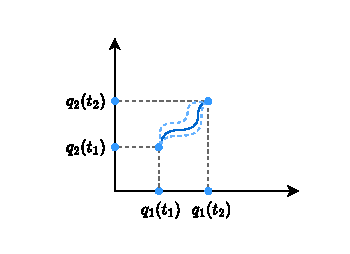
\includegraphics[width=0.6\linewidth]{res/svg/leastactionpath.drawio}
    \caption{Path of least action}
    \label{fig:image9}
\end{figure}
Then \textbf{Hamilton's principle} states that:
\begin{quote} \label{q:Hamilton_principle_quote} %Need to add principle ambient
    The path followed by a monogenic system in configuration space between $t_1$ and $t_2$ is the one for which the action $\action$ is stationary
\end{quote}
The action is defined as:
\begin{equation}
    \action = \int_{t_1}^{t_2}\lagr(q_{\alpha},\dot{q}_{\alpha},t) \dd{t}
\end{equation}
The units for actions are $[\action] = \mathrm{J\cdot s}$.\\ $\action$ is a \underline{functional} which is a "number" that depends on $q_{\alpha}$. Saying that $\action$ is stationary means that slightly changing the path does not change the action.\\
Now we aim to prove that the \hyperref[q:Hamilton_principle_quote]{Hamilton's principle} is true if and only if the \eleref\;are true.\\
\underline{Proof} H.P. $\Rightarrow$ E.L.E.\\
Let's give some conditions:
\begin{itemize}
    \item Call $\Gamma$ the real path
    \item Fix $t_1$ and $t_2$ but sligthly change the path in between
\end{itemize}
For the second point we need to change the real path of a small virtual displacement:
\begin{equation}
    q_{\alpha}(t) \longrightarrow q_{\alpha}(t) + \delta q_{\alpha}(t)
\end{equation}
However after varying the whole path, for the real path we get:
\begin{equation}
    \dot{q}_{\alpha} = \dfrac{\dd{q_{\alpha}}}{\dd{t}}
\end{equation}
for the changed path instead:
\begin{equation}
    \begin{split}
      \dot{q}_{\alpha} + \delta \dot{q}_{\alpha}(t) &= \dv{}{t}\brackets{q_{\alpha}(t) + \delta q_{\alpha}(t)} \\[8pt]
      \cancel{\dot{q}_{\alpha}} + \delta \dot{q}_{\alpha}(t) &= \cancel{\dot{q}_{\alpha}} + \dv{}{t}\brackets{\delta q_{\alpha}(t)} \\[8pt]
      \delta \dot{q}_{\alpha}(t) &= \dv{}{t}\brackets{\delta q_{\alpha}(t)}
    \end{split}
\end{equation}
Now let's evaluate the change on $\action$ and apply \hpquoteref\;which can be mathematically expressed as follows.\\\textbf{Hamilton's principle}:
\begin{equation} \label{e:Hamilton_principle}
    \delta \action = 0
\end{equation}
For the real path:
\begin{equation}
    \action = \int_{t_1}^{t_2}\lagr(q_{\alpha},\dot{q}_{\alpha},t) \dd{t}
\end{equation}
For the changed path:
\begin{equation}
    \tilde{\action} = \int_{t_1}^{t_2}\lagr(q_{\alpha}+\delta q_{\alpha},\dot{q}_{\alpha} + \delta \dot{q}_{\alpha},t) \dd{t}
\end{equation}
And so we get:
\begin{equation}
    \delta \action = \tilde{\action} - \action = \int_{t_1}^{t_2}\brackets{\lagr(q_{\alpha}+\delta q_{\alpha},\dot{q}_{\alpha} + \delta \dot{q}_{\alpha},t) - \lagr(q_{\alpha},\dot{q}_{\alpha},t)} \dd{t}
\end{equation}
The right-hand side of the equation basically has the numerator of the difference quotient:
\begin{equation}
    f'(x)h \sim f(x+h) - f(x)
\end{equation}
for arbitrarily small values of h, which in our case is the value of the virtual displacement $\delta$. Hence, we get:
\begin{equation}
    \delta \action = \int_{t_1}^{t_2}\bigsum_{\alpha}\brackets{\pdv{\lagr}{q_{\alpha}}\delta q_{\alpha} + \pdv{\lagr}{\dot{q}_{\alpha}} \underbrace{\delta \dot{q}_{\alpha}}_{\frac{\dd{}}{\dd{t}}\delta q_{\alpha}}} \dd{t} = 0
\end{equation}
Let's evaluate the second using integration by parts:
\begin{equation}
    \int_{t_1}^{t_2}\bigsum_{\alpha}\pdv{\lagr}{\dot{q}_{\alpha}} \dv{}{t}\delta q_{\alpha} \dd{t} = \cancel{\bigsum_{\alpha}\pdv{\lagr}{\dot{q}_{\alpha}} \delta q_{\alpha}\bigg|_{t_1}^{t_2}} - \int_{t_1}^{t_2}\bigsum_{\alpha}\dv{}{t}\brackets{\pdv{\lagr}{\dot{q}_{\alpha}}} \delta q_{\alpha} \dd{t}
\end{equation}
The term cancelled is zero since the displacement is zero in $t_1$ and $t_2$ for hypotesis. Hence, we get:
\begin{equation}
    \int_{t_1}^{t_2}\bigsum_{\alpha}\pdv{\lagr}{q_{\alpha}}\delta q_{\alpha} \dd{t} - \int_{t_1}^{t_2}\bigsum_{\alpha}\dv{}{t}\brackets{\pdv{\lagr}{\dot{q}_{\alpha}}} \delta q_{\alpha} \dd{t} = 0
\end{equation}
Since all the $\delta q_{\alpha}$ are independent we can pick any index $k$ and say that all the virtual displacements are zero except for the $k$-displacement, and we get:
\begin{equation}
    \int_{t_1}^{t_2}\dfrac{\partial \lagr}{\partial q_{k}}\delta q_{k} \dd{t} - \int_{t_1}^{t_2}\dv{}{t}\brackets{\dfrac{\partial \lagr}{\partial \dot{q}_{k}}} \delta q_{k} \dd{t} = 0
\end{equation}
Now we need a result which is called \textbf{Fundamental Lemma of the calculus of variation} which states that:\\
Taking any continuous function $M\in\mathcal{C}^0([a,b])$ and any function $\eta \in \mathcal{C}^2([a,b])$ such that $\eta(a) = \eta(b) = 0$ then it is true that:
\begin{equation} \label{e:Fundamental_lemma_variation_calculus}
    \int_{a}^{b}M(x)\eta(x)\dd{x} = 0 \Rightarrow M(x) = 0
\end{equation}
For the proof of this lemma we refer to the section (TBD).\\
In our case \eqref{e:Fundamental_lemma_variation_calculus} is satisfied for:
\begin{equation}
    \int_{t_1}^{t_2}\underbrace{\left[\dfrac{\partial \lagr}{\partial q_{k}} - \dv{}{t}\brackets{\dfrac{\partial \lagr}{\partial \dot{q}_{k}}}\right]}_{M} \underbrace{\delta q_{k}}_{\eta} \dd{t} = 0
\end{equation}
Hence:
\begin{equation}
    \begin{split}
      &\pdv{\lagr}{q_{\alpha}} - \dv{}{t}\brackets{\pdv{\lagr}{\dot{q}_{\alpha}}} = 0 \\[8pt]
      &\pdv{\lagr}{q_{\alpha}} = \dv{}{t}\brackets{\pdv{\lagr}{\dot{q}_{\alpha}}}
    \end{split}
\end{equation}
For any arbitrary $\alpha$. Hence, we proved that \hpquotemath\;implies \eleref.\\
It's trivial to prove the opposite since, repeating the passages of the first proof we arrive to:
\begin{equation}
    \delta \action = \int_{t_1}^{t_2}\bigsum_{\alpha}\left[\pdv{\lagr}{q_{\alpha}} - \dv{}{t}\brackets{\pdv{\lagr}{\dot{q}_{\alpha}}}\right] \delta q_{\alpha}
\end{equation}
But the terms in the brackets are all zero because of the \eleref. So we get:
\begin{equation}
    \delta \action = 0
\end{equation}
Which is precisely \hpquotemath.\\
Now that we established the relations between the \eleref\;and the \hpquotemath\;we are ready to prove that if $\lagr$ is a Lagrangian:
\begin{equation}
    \tilde{\lagr} = \lagr + \dfrac{\dd{F}}{\dd{t}}
\end{equation}
is a Lagrangian for the system. Evaluating the action for both Lagrangians we get:
\begin{equation}
    \tilde{\action} = \int_{t_1}^{t_2}\lagr \dd{t} + \int_{t_1}^{t_2}\dfrac{\dd{F}}{\dd{t}} \dd{t}
\end{equation}
\begin{equation}
    \action = \int_{t_1}^{t_2}\lagr \dd{t}
\end{equation}
The difference of action for the new Lagrangian is:
\begin{equation}
    \delta \tilde{\action} = \int_{t_1}^{t_2}\dfrac{\dd{F}}{\dd{t}} \dd{t} = F(t_2) - F(t_1)
\end{equation}
And so we get:
\begin{equation}
    \delta \tilde{\action} = \delta \action + \cancel{\delta(F(t_2) - F(t_1))}
\end{equation}
The variation between the values of $F$ is obviously zero since their difference is just a constant number that comes from the integral. So if \hpquotemath\;holds for $\lagr$ we have:
\begin{equation}
    \delta \tilde{\action} = \delta \action = 0
\end{equation}
And so $\tilde{\lagr}$ is a Lagrangian for the system.\\
\section{Examples (WIP)}
\section{The energy function}
Let's now discuss the energy of a system. The Lagrangian $\lagr$ has the dimensions of an energy, but it \underline{is not} the total energy.
\begin{equation}
    \lagr = T - V \cancel{\Leftrightarrow} E = T + V
\end{equation}
We can evaluate the derivative of the Lagrangian and see what we get:
\begin{equation}
    \dfrac{\dd{\lagr}}{\dd{t}} = \bigsum_{\alpha}\brackets{\pdv{\lagr}{q_{\alpha}}\dot{q}_{\alpha} + \pdv{\lagr}{\dot{q}_{\alpha}}\ddot{q}_{\alpha}} + \dfrac{\partial \lagr}{\partial t}
\end{equation}
If \eleref\;hold then we have:
\begin{equation}
    \dfrac{\dd{\lagr}}{\dd{t}} = \bigsum_{\alpha}\underbrace{\left[\dv{}{t}\brackets{\pdv{\lagr}{\dot{q}_{\alpha}}}\dot{q}_{\alpha} + \pdv{\lagr}{\dot{q}_{\alpha}}\ddot{q}_{\alpha}\right]}_{\text{total time derivative}} + \dfrac{\partial \lagr}{\partial t} =
\end{equation}
\begin{equation}
 = \dv{}{t}\bigsum_{\alpha}\pdv{\lagr}{\dot{q}_{\alpha}}\dot{q}_{\alpha} + \dfrac{\partial \lagr}{\partial t}
\end{equation}
So in general:
\begin{equation}
    \dfrac{\dd{\lagr}}{\dd{t}} \neq 0
\end{equation}
even if the partial derivative of $\lagr$ with respect to time is zero. But we can define a quantity $h$ called \textbf{energy function}:
\begin{equation}
    h \defineeq \bigsum_{\alpha}\pdv{\lagr}{\dot{q}_{\alpha}}\dot{q}_{\alpha} - \lagr
\end{equation}
and so we have:
\begin{equation}
    \dfrac{\dd{h}}{\dd{t}} = -\dfrac{\partial \lagr}{\partial t}
\end{equation}
Obviously $h$ is a constant of motion if and only if the partial derivative with respect to time of the Lagrangian is 0:
\begin{equation}
    h\;\text{is conserved} \iff \dfrac{\dd{h}}{\dd{t}} = 0 \iff \dfrac{\partial \lagr}{\partial t} = 0
\end{equation}
Saying that $\lagr$ does not depend on time explicitly means that the potential $V$ does not depend on time and also:
\begin{itemize}
    \item Constraints depending on time $\Rightarrow$ $\lagr$ depends on time
    \item Constraints not depending on time $\Rightarrow$ $\lagr$ does not depend on time
\end{itemize}
Now we want to prove that $h$ is the total energy if these conditions hold:
\begin{enumerate}
    \item Transformation equations do not depend on time
    \item The potential $V$ does not depend on time
\end{enumerate}
Let's further analyse condition (1). Writing the kinetic energy $T$ we get:
\begin{equation}
    T = \dfrac{1}{2}\bigsum_i m_i v_i^2 = \dfrac{1}{2}\bigsum_i m_i \dvec{r}_i \cdot \dvec{r}_i
\end{equation}
The time derivative of $r_i(q_{\alpha},t)$ is:
\begin{equation}
    \dvec{r}_i = \dfrac{\dd{\vec{r}_i}}{\dd{t}} = \bigsum_{\alpha}\dfrac{\partial \vec{r}_i}{\partial q_{\alpha}}\dot{q}_{\alpha} + \dfrac{\partial \vec{r}_i}{\partial t}
\end{equation}
Hence we have:
\begin{equation}
    T = \dfrac{1}{2}\bigsum_i m_i \left[\bigsum_{\alpha}\dfrac{\partial \vec{r}_i}{\partial q_{\alpha}}\dot{q}_{\alpha} + \dfrac{\partial \vec{r}_i}{\partial t}\right] \cdot \left[\bigsum_{\beta}\dfrac{\partial \vec{r}_i}{\partial q_{\beta}}\dot{q}_{\beta} + \dfrac{\partial \vec{r}_i}{\partial t}\right] =
\end{equation}

\begin{equation}
    \begin{split}
        = \dfrac{1}{2}\bigsum_i m_i \bigsum_{\alpha}\bigsum_{\beta}\dfrac{\partial \vec{r}_i}{\partial q_{\alpha}}\cdot\dfrac{\partial \vec{r}_i}{\partial q_{\beta}}\dot{q}_{\alpha}\dot{q}_{\beta} + \dfrac{1}{2}\bigsum_i m_i \dfrac{\partial \vec{r}_i}{\partial t} \cdot \dfrac{\partial \vec{r}_i}{\partial t} +\\
        + \dfrac{1}{2}\bigsum_i m_i \bigsum_{\alpha}\dfrac{\partial \vec{r}_i}{\partial q_{\alpha}} \cdot \dfrac{\partial \vec{r}_i}{\partial t} \dot{q}_{\alpha} + \dfrac{1}{2}\bigsum_i m_i \bigsum_{\beta}\dfrac{\partial \vec{r}_i}{\partial q_{\beta}} \cdot \dfrac{\partial \vec{r}_i}{\partial t}\dot{q}_{\beta}
    \end{split}
\end{equation}
The terms on the second line are actually the same since summing over $\alpha$ or $\beta$ is actually the same. Let us now define some quantities for a shorter notation:
\begin{equation}
    \begin{split}
        T_{\alpha \beta} \defineeq \bigsum_i m_i \dfrac{\partial \vec{r}_i}{\partial q_{\alpha}}\cdot\dfrac{\partial \vec{r}_i}{\partial q_{\beta}}\\
        T_{\alpha} \defineeq \dfrac{1}{2} \bigsum_i m_i \dfrac{\partial \vec{r}_i}{\partial q_{\alpha}} \cdot \boxed{\dfrac{\partial \vec{r}_i}{\partial t}}\\
        T_0 \defineeq \dfrac{1}{2}\bigsum_i m_i \boxed{\dfrac{\partial \vec{r}_i}{\partial t} \cdot \dfrac{\partial \vec{r}_i}{\partial t}}
    \end{split}
\end{equation}
The quantities $T_{\alpha}$ and $T_0$ are zero if the transformation equations do not depend on time explicitly since the partial derivative with respect to time of $\vec{r}_i$ is zero. Rewriting the kinetic energy we have:
\begin{equation}
    T = \dfrac{1}{2}\bigsum_{\alpha}\bigsum_{\beta}T_{\alpha \beta}\dot{q}_{\alpha}\dot{q}_{\beta} + \cancel{\bigsum_{\alpha}T_{\alpha}\dot{q}_{\alpha}} + \cancel{T_0}
\end{equation}
\begin{equation} \label{e:kinetic_energy}
    T = \dfrac{1}{2}\bigsum_{\alpha}\bigsum_{\beta}T_{\alpha \beta}\dot{q}_{\alpha}\dot{q}_{\beta}
\end{equation}
And so $T$ is a quadratic function of the generalized velocities.\\
Now let's analyse condition (2). To start we can remember this:
\begin{equation}
    \pdv{\lagr}{\dot{q}_{\alpha}} = \dfrac{\partial T}{\partial \dot{q}_{\alpha}} - \cancel{\partial{V}{\dot{q}_{\alpha}}}
\end{equation}
since $V$ does not depend on the generalized velocities. Now substituting \eqref{e:kinetic_energy} we get:
\begin{equation}
    h = \bigsum_{\gamma}\dfrac{\partial T}{\partial \dot{q}_{\gamma}} - \lagr = \bigsum_{\gamma}\dfrac{\partial}{\partial \dot{q}_{\gamma}}\bbrackets{\dfrac{1}{2}\bigsum_{\alpha}\bigsum_{\beta}\underbrace{T_{\alpha \beta}}_{\cancel{\propto} \dot{q}_{\alpha}, \dot{q}_{\beta}}\dot{q}_{\alpha}\dot{q}_{\beta}}  - \lagr =
\end{equation}
We can bring the partial derivative inside the sum:
\begin{equation}
    h = \dfrac{1}{2}\bigsum_{\gamma}\bigsum_{\alpha}\bigsum_{\beta}T_{\alpha \beta}\bbrackets{\underbrace{\dfrac{\partial \dot{q}_{\alpha}}{\partial \dot{q}_{\gamma}}}_{\delta_{\alpha \gamma}}\dot{q}_{\beta} + \underbrace{\dfrac{\partial \dot{q}_{\beta}}{\partial \dot{q}_{\gamma}}}_{\delta_{\beta \gamma}}\dot{q}_{\alpha}} - \lagr
\end{equation}
If we split out the terms of the sum we can cancel out the sum over $\alpha$ in the first term due to the Kronecker delta. Similarly, we can cancel out the sum over $\beta$. We need to remind that we also need to switch the cancelled indexes with $\gamma$ since those are the remaining terms.
\begin{equation}
    \bigsum_{\gamma}\cancel{\bigsum_{\alpha}}\bigsum_{\beta}T_{\alpha \beta }\cancel{\delta_{\alpha \gamma}}\dot{q}_{\beta} = \bigsum_{\gamma}\bigsum_{\beta}T_{\gamma \beta }\dot{q}_{\beta}
\end{equation}
So we get:
\begin{equation}
    h = \underbrace{\dfrac{1}{2}\bigsum_{\gamma}\bigsum_{\beta}T_{\gamma \beta }\dot{q}_{\beta}}_{T} + \underbrace{\dfrac{1}{2}\bigsum_{\gamma}\bigsum_{\alpha}T_{\gamma \alpha }\dot{q}_{\alpha}}_{T} - \lagr = 2T - (T-V) = T + V = E
\end{equation}
And so conditions (1) and (2) really are the conditions for $h$ to be the total energy of the system $E$. The conditions for $h$ to be the energy and for $h$ to be conserved do not necessarily match, so we can have all the possible cases:
\begin{itemize}
    \item $h$ is the energy and it is conserved
    \item $h$ is the energy but it is not conserved
    \item $h$ is not the energy but it is conserved
    \item $h$ is not the energy and it is not conserved
\end{itemize}
\section{Conservation of the total linear momentum}
Let's now talk about the conservation of linear momenta. In the Lagrange formalism the role of linear momentum is done by the \textbf{generalized momentum} conjugate to $q_{\alpha}$:
\begin{equation}
    p_{\alpha} \defineeq \pdv{\lagr}{\dot{q}_{\alpha}}
\end{equation}
which can also be called \textbf{canonical momentum}. The generalized momentum may not correspond to the linear momentum we get from Newton's equations. We can show that for an easy example the two quantities correspond.\\
Let's define the Lagrangian as:
\begin{equation}
    \lagr = \dfrac{1}{2}m(\dot{x}^2 + \dot{y}^2 + \dot{z}^2) - V(x,y,z)
\end{equation}
This might be an example for an easy "Physics I-like" system (for example a falling object). We evaluate the generalized momentum conjugate to x and get:
\begin{equation}
    p_x = \dfrac{\partial \lagr}{\partial \dot{x}} = m\dot{x}
\end{equation}
which is indeed the linear momentum found by using Newton's equations.\\
If we go back to \eleref\;and \lagrangeref\;we can identify the term $p_{\alpha}$ inside those equations. If they hold (remember we need to ask for a potential independent of the velocities) then we can write:
\begin{equation}
    \dfrac{\dd{p_{\alpha}}}{\dd{t}} = \pdv{\lagr}{q_{\alpha}} \Rightarrow \dot{p}_{\alpha} = \pdv{\lagr}{q_{\alpha}}
\end{equation}
If only the potential does depend on the coordinates and $T$ does not then we can also write:
\begin{equation}
    \dot{p}_{\alpha} = \pdv{[\cancel{T}-V]}{q_{\alpha}} = -\pdv{V}{q_{\alpha}}
\end{equation}
If $V$ does not depend on the velocities we also have:
\begin{equation}
    -\pdv{V}{q_{\alpha}} = Q_{\alpha}
\end{equation}
\begin{equation}
    \boxed{\dot{p}_{\alpha} = Q_{\alpha}}
\end{equation}
This is the corresponding relation for $\vec{F} = \dvec{p}$ in Newton's equations. If $V$ depends on $\dot{q}_{\alpha}$ we get:
\begin{equation}
    \dv{}{t}\pdv{V}{\dot{q}_{\alpha}}-\pdv{V}{q_{\alpha}} = Q_{\alpha}
\end{equation}
Let us now define what \textbf{cyclic coordinates} are.
\begin{equation}
    q_{\alpha}\;\text{is cyclic} \iff \pdv{\lagr}{q_{\alpha}} = 0
\end{equation}
If $q_{\alpha}$ is cyclic and \eleref\;are true we have:
\begin{equation}
    \dv{}{t} \pdv{\lagr}{\dot{q}_j} - \cancel{\pdv{\lagr}{q_{\alpha}}} = 0
\end{equation}
\begin{equation}
    \dot{p}_{\alpha} = 0
\end{equation}
This means that if a coordinate is cyclic its corresponding generalized momentum is conserved.\\
Now let $q_j$ be a \textbf{collective coordinate} such that $\delta q_j$ represents an infinitesimal displacement of the system \underline{as a whole}.
\begin{figure}[H]
    \centering
    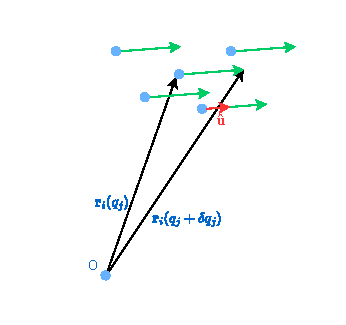
\includegraphics[width=0.4\linewidth]{res/svg/collectivecoord.drawio}
    \caption{Collective coordinate}
\end{figure}
If this is the case all the particles are moving parallel to a single unit vector $\hat{u}$:
\begin{equation}
    \hat{u} = \dfrac{\partial \vec{r}_i}{\partial q_j}
\end{equation}
\begin{equation}
    \delta \vec{r}_i = \delta q_j \hat{u}
\end{equation}
Also $q_j$ cannot appear in the expression of $T$, hence:
\begin{equation}
    \pdv{T}{q_j}=0
\end{equation}
Changing $q_j$ is a translation that leaves everything untouched (like moving the origini of the axis). Now consider $V=V(q_{\alpha},\cancel{\dot{q}_{\alpha}},t)$:
\begin{equation}
    -\pdv{V}{q_{\alpha}} = Q_{\alpha}
\end{equation}
Let's consider \eleref\;for $q_j$:
\begin{equation}
    \dv{}{t}\underbrace{\pdv{\lagr}{\dot{q}_j}}_{p_j} - \underbrace{\pdv{\lagr}{q_j}}_{-\frac{\partial V}{\partial q_j}} = 0
\end{equation}
\begin{equation} \label{e:ele_for_qj}
    \dv{}{t}p_j = -\pdv{V}{q_j} = Q_j
\end{equation}
Remembering the definition of $Q_j$:
\begin{equation}
    Q_j = \bigsum_i \vec{F}_i \cdot \underbrace{\pdv{\vec{r}_i}{q_j}}_{\hat{u}} = \vec{F}\cdot \hat{u}
\end{equation}
Similarly from the definition of $p_j$:
\begin{equation}
    p_j = \pdv{\lagr}{\dot{q}_j} = \pdv{}{\dot{q}_j}\brackets{\dfrac{1}{2}\bigsum_i m_i \vec{r}_i^{\;2}} = \dfrac{1}{2}\bigsum_i m_i \pdv{}{\dot{q}_j}(\vec{r}_i^2) = \bigsum_i m_i \vec{r}_i \cdot \underbrace{\pdv{\vec{r}_i}{\dot{q}_j}}_{\hat{u}}
\end{equation}
\begin{equation}
    p_j = \vec{P}\cdot\hat{u}
\end{equation}
Going back to \eqref{e:ele_for_qj}:
\begin{equation}
    \dv{}{t}(\vec{P}\cdot\hat{u}) = \vec{F}\cdot \hat{u}
\end{equation}
If $q_j$ is also a cyclic coordinate we have:
\begin{equation}
    \pdv{\lagr}{q_j} = 0 \Rightarrow \pdv{[\cancel{T}-V]}{q_j} = \pdv{V}{q_j} = 0
\end{equation}
From this immediately follows:
\begin{equation}
    Q_j = 0 \Rightarrow \dv{}{t}(p_j) = \dv{}{t}(\vec{P}\cdot\hat{u}) = 0
\end{equation}
So if $q_j$ is a cyclic and collective coordinate the generalized momentum conjugate to $q_j$ si conserved.
\section{Conservation of the total angular momentum}
Let's consider a specific coordinate $q_j$ such that $\delta q_j$ is a rigid rotation of the system as a whole, about a certain axis as shown:
\\\textbf{IMAGE}\\
We can see that $\delta \vec{r}_i$ is a tangential displacement. If we use the angle $\theta$ as our coordinate we can write:
\begin{equation}
    \dv{\vec{r}_i}{t} = \dv{\theta}{t} \hat{u} \cross \vec{r}_i = \dot{q}_j \hat{u} \cross \vec{r}_i
\end{equation}
From which follows:
\begin{equation}
    \delta \vec{r}_i = \delta q_j \hat{u} \cross \vec{r}_i \Rightarrow \pdv{\vec{r}_i}{q_j} = \hat{u} \cross \vec{r}_i
\end{equation}
Also $q_j$ cannot appear in the expression of $T$, hence:
\begin{equation}
    \pdv{T}{q_j} = 0
\end{equation}
Now we consider a system such that $V = V(q_{\alpha},\cancel{\dot{q}_{\alpha}},t)$ and write \eleref\;for $q_j$:
\begin{equation} \label{e:ele_for_angular_momentum}
    \begin{split}
        \dv{}{t}\pdv{\lagr}{\dot{q}_j} - \pdv{\lagr}{q_j} = 0\\
        \dv{}{t}\underbrace{\pdv{T}{\dot{q}_j}}_{p_j} - \bbrackets{\underbrace{- \pdv{V}{q_j}}_{Q_j}} = 0
    \end{split}
\end{equation}
Let's explicitly write $Q_j$:
\begin{equation}
    Q_j = \bigsum_i \vec{F}_i \cdot \pdv{\vec{r}_i}{q_j} = \bigsum_i \vec{F}_i \cdot \hat{u} \cross \vec{r}_i
\end{equation}
Inside the summation we have a triple product, hence we can exploit the fact that $\hat{u}$ does not depend on $i$ and also the invariance of the triple product with respect to circular shifts:
\begin{equation}
    \vec{a} \cdot \vec{b} \cross \vec{c} = \vec{c} \cdot \vec{a} \cross \vec{b} = \vec{b} \cdot \vec{c} \cross \vec{a}
\end{equation}
And so we get:
\begin{equation}
    Q_j = \hat{u} \cdot \underbrace{\bigsum_i \vec{r}_i \cross \vec{F}_i}_{\vec{\tau}} = \hat{u} \cdot \vec{\tau}
\end{equation}
Now let's analyse the partial derivative of the kinetic energy:
\begin{equation}
    \pdv{T}{\dot{q}_j} = \pdv{}{\dot{q}_j}\brackets{\dfrac{1}{2}\bigsum_i m_i \vec{r}_i^{\;2}} = \bigsum_i m_i \vec{r}_i \cdot \pdv{\vec{r}_i}{\dot{q}_j} = \bigsum_i m_i \vec{r}_i \cdot \hat{u} \cross \vec{r}_i
\end{equation}
Again we exploit the properties of the triple product and get:
\begin{equation}
    \pdv{T}{\dot{q}_j} =   \hat{u} \cdot \underbrace{\bigsum_i \vec{r}_i \cross m_i \vec{r}_i}_{\vec{L}_0} = \hat{u} \cdot \vec{L}_0
\end{equation}
Finally we can substitute back into \eqref{e:ele_for_angular_momentum}:
\begin{equation}
    \dv{}{t}\brackets{\vec{L}_0 \cdot \hat{u}} = \vec{\tau} \cdot \hat{u}
\end{equation}
This means that if the total torque about a generic axis is zero, then the total angular momentum about that axis is conserved. For example if we let $\hat{u} = \hat{z}$:
\begin{equation}
    \tau_z = 0 \Rightarrow L_z\;\text{is conserved}
\end{equation}
We then notice that if $q_j$ is a cyclic coordinate we have:
\begin{equation}
    Q_j = -\pdv{V}{q_j} = 0 \Rightarrow \vec{\tau} \cdot \hat{u} = 0 \Rightarrow \vec{L}_0 \cdot \hat{u}\;\text{is conserved}
\end{equation}
\section{Noether's theorem}
In the last two sections we arrived to these conclusions:
\begin{itemize}
    \item The conservation of the total momentum is due to an invariance of $\lagr$ to translations
    \item The conservation of the momentum along an axis is due to an invariance of $\lagr$ to translation along that axis
    \item The conservation of the total angular momentum is due to an invariance of $\lagr$ to rotations
    \item The conservation of the angular momentum along an axis is due to an invariance of $\lagr$ to rotations along that axis
    \item If $\lagr$ is invariant with respect to time the energy function is conserved
\end{itemize}
We can easily see the "pattern" arising from those conclusions. Those are all examples of a famous theorem which states:
\begin{theorem}{Noether's theorem}
    For every invariance of $\lagr$ there is a conserved quantity
\end{theorem}

\chapter{Hamilton's mechanics}
\section{Hamilton's equations}
Now let's recap what we established with the differente pictures of classical mechanics that we discussed until now.
\begin{itemize}
    \item \eleref\;are a set of $n$ differential equations of $2^\circ$ order with $2n$ initial conditions
    \item When a coordinate is cyclic then: \begin{equation}
        p_{\alpha} = \pdv{\lagr}{\dot{q}_{\alpha}}\;\text{is conserved}
    \end{equation}
    but $p_{\alpha}$ is not a quantity of the Lagrangian
    \item even if $p_\alpha$ is conserved we still have $\dot{q}_{\alpha}$ as an ``extra'' term in the Lagrangian
\end{itemize}
We want to use a space differente from the configuration space in order to get rid of a useless term when a coordinate is cyclic. We then introduce a new concept.
\begin{definition}{Phase space}
  Phase space is a $2n$-dimensional space in which each point represents the \underline{state} of the system $\{q_{\alpha},p_{\alpha}\}$.
\end{definition}
Here are the fundamental differences between Lagrange formulation and Hamilton formulation of classical mechanics:
\begin{table}[H]
    \centering
    \begin{tabular}{lll}
        \underline{Lagrange} & $\longrightarrow$ &\underline{Hamilton}\\[8pt]
        $\lagr=\lagr(q_{\alpha},\dot{q}_{\alpha},t)$ & &$\hamfun=\hamfun(q_{\alpha},p_{\alpha},t)$\\[8pt]
        Configuration space & &Phase space\\[8pt]
        $n$ dimensions & &$2n$ dimensions
    \end{tabular}
\end{table}
Since we want to find a new function related to the Lagrangian that contains $p_{\alpha}$ as a variable instead of $\dot{q}_{\alpha}$, we need to introduce a certain type of transformation.\\
\textbf{Legendre transformations} are able to write a function $f(x,y)$ as a function $g(u,y)$ where:
\begin{equation}
    \dd{f} = \underbrace{\pdv{f}{x}}_u \dd{x} + \underbrace{\pdv{f}{y}}_v \dd{y} = u\dd{x} + v\dd{y}
\end{equation}
From this first relation we can work on the term $u\dd{x}$:
\begin{equation}
    \dd{(ux)} = u\dd{x} + x\dd{u} \Rightarrow u\dd{x} = \dd{(ux)} - x\dd{u}
\end{equation}
Then it is easy to see that a function $g = f-ux$ satisfies our conditions, and so we have:
\begin{equation}
    \dd{g} = \dd{(f-ux)} = - x\dd{u} + v\dd{y} \Rightarrow \begin{cases}
        \partial_{u} g = -x\\
        \partial_{y} g = v
    \end{cases}
\end{equation}
Let's try to apply Légendre transformations to the Lagrangian:
\begin{equation}
    \dd{\lagr} = \bigsum_{\alpha} \pdv{\lagr}{q_{\alpha}}\dd{q_{\alpha}} + \bigsum_{\alpha} \underbrace{\pdv{\lagr}{\dot{q}_{\alpha}}}_{p_{\alpha}}\dd{\dot{q}_{\alpha}} + \pdv{\lagr}{t}\dd{t}
\end{equation}
We then applied Légendre transformations to $\lagr$:
\begin{equation} \label{e:legendre_hamilton}
    \dd{\brackets{\lagr - \bigsum_{\alpha} p_{\alpha}\dot{q}_{\alpha}}} = \bigsum_{\alpha} \pdv{\lagr}{q_{\alpha}}\dd{q_{\alpha}} - \bigsum_{\alpha} \dot{q}_{\alpha}\dd{p_{\alpha}} + \pdv{\lagr}{t}\dd{t}
\end{equation}
And so if we define a function $\hamfun$ called \textbf{Hamiltonian} (or Hamilton function):
\begin{equation}
    \hamfun \defineeq \bigsum_{\alpha} p_{\alpha}\dot{q}_{\alpha} -\lagr
\end{equation}
Then \eqref{e:legendre_hamilton} becomes:
\begin{equation}
    \begin{split}
        -\dd{\hamfun} = \bigsum_{\alpha} \underbrace{\pdv{\lagr}{q_{\alpha}}}_{\dot{p}_{\alpha}}\dd{q_{\alpha}} - \bigsum_{\alpha} \dot{q}_{\alpha}\dd{p_{\alpha}} + \pdv{\lagr}{t}\dd{t}\\
        \dd{\hamfun} = -\bigsum_{\alpha} \dot{p}_{\alpha}\dd{q_{\alpha}} + \bigsum_{\alpha} \dot{q}_{\alpha}\dd{p_{\alpha}} - \pdv{\lagr}{t}\dd{t}\\
    \end{split}
\end{equation}
But also it is genrally true that:
\begin{equation}
    \dd{\hamfun} = \bigsum_{\alpha} \pdv{\hamfun}{q_{\alpha}}\dd{q_{\alpha}} + \bigsum_{\alpha} \pdv{\hamfun}{p_{\alpha}}\dd{p_{\alpha}} + \pdv{\hamfun}{t}\dd{t}
\end{equation}
The two equations must be equal so we get \textbf{Hamilton's canonical equations}:
\begin{equation} \label{hamilton_equations}
    \boxed{
    \begin{aligned}
        \pdv{\hamfun}{q_{\alpha}} &= -\dot{p}_{\alpha}\\
        \pdv{\hamfun}{p_{\alpha}} &=\;\;\;\dot{q}_{\alpha}\\
        \pdv{\hamfun}{t} &= -\pdv{\lagr}{t}
    \end{aligned}}
\end{equation}
This is a system of $2n (+1)$ equations, but they are first order ODEs so we have $2n$ initial conditions as in \lagrangeref. With this formulation we have one important advantage: if $q_j$ is cyclic then $\dot{p} = 0$, and we don't need to solve one of the differential equations.
This means that we only need $2n-1$ initial conditions. Same goes for any other cyclic coordinate, and so we have $2n-p$ initial conditions with $p$ being the number of cyclic coordinates.\\
Now let's remember the definition of the energy function:
\begin{equation}
    h = \bigsum_{\alpha}\underbrace{\pdv{\lagr}{q_{\alpha}}}_{p_{\alpha}}\dot{q}_{\alpha} - \lagr
\end{equation}
So we can say that the only difference between the energy function $h$ and the Hamiltonian $\hamfun$ is the fact that the first lives in the configuration space, the latter instead lives in the phase space.
To further convince ourselves of this fact we can evaluate the total derivative of $\hamfun$ over time:
\begin{equation}
    \begin{split}
        \dv{\hamfun}{t} &= \bigsum_{\alpha}\underbrace{\pdv{\hamfun}{q_{\alpha}}}_{-\dot{p}_{\alpha}}\dot{q}_{\alpha} + \bigsum_{\alpha}\underbrace{\pdv{\hamfun}{p_{\alpha}}}_{\dot{q}_{\alpha}}\dot{p}_{\alpha} + \pdv{\hamfun}{t} \\
        \dv{\hamfun}{t} &= \pdv{\hamfun}{t} = -\pdv{\lagr}{t}
    \end{split}
\end{equation}
So we get that $\hamfun$ will be the energy and/or will be conserved in the same situations of the energy function.
\section{Hamilton's equations through Hamilton's principle}
To derive \hamiltonref\;we can also exploit \hpquotemath\;starting from:
\begin{equation}
    \action = \int_{t_1}^{t_2}\lagr \dd{t}
\end{equation}
Using the same definition for $\hamfun$ that we previously used:
\begin{equation}
    \hamfun = \bigsum_{\alpha}p_{\alpha}\dot{q}_{\alpha} - \lagr
\end{equation}
We get:
\begin{equation} \label{e:deltaS_hamilton}
    \delta \action = \int_{t_1}^{t_2}\bbrackets{\bigsum_{\alpha}\delta p_{\alpha}\dot{q}_{\alpha} + \bigsum_{\alpha} p_{\alpha} \underbrace{\delta \dot{q}_{\alpha}}_{\frac{\dd{}}{\dd{t}}\delta q_{\alpha}} - \bigsum_{\alpha} \pdv{\hamfun}{q_{\alpha}} \delta q_{\alpha}- \bigsum_{\alpha} \pdv{\hamfun}{p_{\alpha}} \delta p_{\alpha}} \dd{t}
\end{equation}
We apply the product rule on the second member:
\begin{equation}
    \bigsum_{\alpha} p_{\alpha} \dv{}{t}\delta q_{\alpha} = \bigsum_{\alpha} \bigg[ \dv{}{t} \brackets{p_{\alpha} \delta q_{\alpha}} -  \delta q_{\alpha}\dv{}{t}p_{\alpha}\bigg]
\end{equation}
Integrating the first term we get:
\begin{equation}
    \int_{t_1}^{t_2} \bigsum_{\alpha} \dv{}{t} \brackets{p_{\alpha} \delta q_{\alpha}} \dd{t} = \bigsum_{\alpha} p_{\alpha} \delta q_{\alpha} \bigg|_{t_1}^{t_2} = 0
\end{equation}
This is zero because in \hpquotemath\;we assumed that the virtual displacement at the extreme points is zero. So we can rewrite \eqref{e:deltaS_hamilton} putting in evidence the common terms:
\begin{equation}
    \begin{split}
        \delta \action &= \int_{t_1}^{t_2}\bbrackets{\bigsum_{\alpha}\delta p_{\alpha}\dot{q}_{\alpha} - \bigsum_{\alpha} \delta q_{\alpha}\dot{p}_{\alpha} - \bigsum_{\alpha} \pdv{\hamfun}{q_{\alpha}} \delta q_{\alpha}- \bigsum_{\alpha} \pdv{\hamfun}{p_{\alpha}} \delta p_{\alpha}} \dd{t} \\
        \delta \action &= \int_{t_1}^{t_2}\bbrackets{\bigsum_{\alpha}\bigg[\dot{q}_{\alpha} - \pdv{\hamfun}{p_{\alpha}}\bigg] \delta p_{\alpha} - \bigsum_{\alpha} \bigg[\dot{p}_{\alpha} + \pdv{\hamfun}{q_{\alpha}} \bigg]\delta q_{\alpha}} \dd{t} = 0
    \end{split}
\end{equation}
Since all the terms are independent by construction all the brackets must be zero. In this way we get the same set of equation as we did before.
\section{Poisson brackets}
In the context of Hamilton's mechanics we can introduce the notion of the \textbf{Poisson brackets}.\\
Consider two functions $f,g$ in the phase space:
\begin{equation}
    \begin{cases}
        f = f(q_{\alpha},p_{\alpha},t)\\
        g = g(q_{\alpha},p_{\alpha},t)
    \end{cases}
\end{equation}
We define Poisson brackets as follows:
\begin{equation}
    \pb{f}{g} = \bigsum_{\alpha}\brackets{\pdv{f}{q_{\alpha}}\pdv{g}{p_\alpha} - \pdv{f}{p_{\alpha}}\pdv{g}{q_{\alpha}}}
\end{equation}
Notice that $\pb{f}{g}$ is still a function in the phase space.\\
Now we can give some \underline{properties} of the Poisson brackets:
\begin{enumerate}
    \item antisimmetry: \[\pb{f}{g} = - \pb{g}{f}\]
    \item bilinearity:
    \[\pb{\alpha f + \beta g}{h} = \alpha\pb{f}{h}+ \beta\pb{g}{h}\]
    \[\pb{h}{\alpha f + \beta g} = \alpha\pb{h}{f}+ \beta\pb{h}{g}\]
    \item Leibniz rule: \[\pb{f}{gh} = g\pb{f}{h} + \pb{f}{g}h\]
    \item Jacobi identity: \[\pb{f}{\pb{g}{h}} + \pb{h}{\pb{f}{g}} + \pb{g}{\pb{h}{f}} = 0\]
\end{enumerate}
Given this definition let's evaluate the total time derivative of a function $f$ in the phase space:
\begin{equation}
    \dv{f}{t} = \bigsum_{\alpha}\brackets{\pdv{f}{q_{\alpha}}\dot{q}_{\alpha} + \pdv{f}{p_{\alpha}}\dot{p}_{\alpha}} + \pdv{f}{t}
\end{equation}
Using \hamiltonref\;we can rewrite this as:
\begin{equation}
    \begin{split}
        \dv{f}{t} &= \bigsum_{\alpha}\brackets{\pdv{f}{q_{\alpha}}\pdv{\hamfun}{p_{\alpha}} - \pdv{f}{p_{\alpha}}\pdv{\hamfun}{q_{\alpha}}} + \pdv{f}{t}\\[8pt]
        \dv{f}{t} &= \pb{f}{\hamfun} + \pdv{f}{t}
    \end{split}
\end{equation}
And so we can get a new condition for any generic function $f$ to be a constant of motion:
\begin{equation}
    f\;\text{is conserved} \iff \dv{f}{t} = 0 \iff \pb{f}{\hamfun} = -\pdv{f}{t}
\end{equation}
Furter more if $f$ is independent of time the condition is:
\begin{equation}
    \pb{f}{\hamfun} = 0
\end{equation}
\section{Examples (WIP)}
\subsection{Ex. 1}
Let us start with a simple example. Consider a unconstrained particle moving on a frictionless plane under the action of a potential $V(x,y)$. We have 2 degrees of freedom. We can simply choose cartesian coordinates and write the Lagrangian:
\begin{equation}
  \lagr = T - V = \dfrac{1}{2}m(\dot{x}^2+\dot{y}^2) - V(x,y)
\end{equation}
Now the conjugated momenta are:
\begin{equation}
  \begin{split}
    &p_x = m\dot{x} \\[8pt]
    &p_y = m\dot{y}
  \end{split}
\end{equation}
And so the Hamiltonian is:
\begin{equation}
  \begin{split}
    \hamfun &= p_x\dot{x} + p_y\dot{y} - \dfrac{1}{2}m(\dot{x}^2+\dot{y}^2) + V(x,y) =\\[8pt]
    &= m(\dot{x}^2+\dot{y}^2) - \dfrac{1}{2}m(\dot{x}^2+\dot{y}^2) + V(x,y) = \dfrac{\vec{p}^2}{2m} + V(x,y)
  \end{split}
\end{equation}
Here $T$ is a quadratic function of the velocities and $V$ does not depend on the velocities, hence $\hamfun = E$ as expected. The first two \hamiltonref\;are:
\begin{equation}
  \begin{split}
    \dot{x} = \pdv{\hamfun}{p_x} = \dfrac{p_x}{m} \\[8pt]
    \dot{y} = \pdv{\hamfun}{p_y} = \dfrac{p_y}{m}
  \end{split}
\end{equation}
Those are already known. We also have that:
\begin{equation}
  \begin{split}
    \dot{p}_x = -\pdv{\hamfun}{x} = -\pdv{V}{x} \\[8pt]
    \dot{p}_y = -\pdv{\hamfun}{y} = -\pdv{V}{y}
  \end{split}
\end{equation}
And so:
\begin{equation}
  \dot{\vec{p}} = -\grad{V} = \vec{F}
\end{equation}
Again we find something that is not new.\\
\subsection{Ex. 2}
\begin{figure}[H]
  \centering
  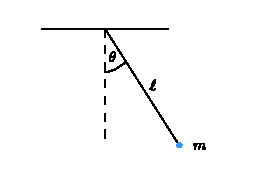
\includegraphics[width=0.5\linewidth]{res/svg/simple_pendulum.drawio}
  \caption{Simple pendulum}
\end{figure}
Now we can discuss the problem of a simple pendulum in the Hamilton formalism. We have a mass $m$ attached to a thin massless rod of length $\ell$. The constraint given by the rod is holonomic and scleronomic:
\begin{equation}
  x^2+y^2-\ell^2 = 0
\end{equation}
We have only one independent coordinate. Let us choose the angle $\theta$. We have that:
\begin{equation}
  \begin{split}
    &x = \ell \cos \theta \implies \dot{x} = - \ell \dot{\theta}\sin \theta \\[8pt]
    &y = \ell \sin \theta \implies \dot{y} = \ell \dot{\theta}\cos \theta
  \end{split}
\end{equation}
The potential is just given by the gravitational potential, which in the reference frame that we fixed is:
\begin{equation}
  V = -mgy = -mg \ell \cos \theta
\end{equation}
The Lagrangian is:
\begin{equation}
  \lagr = \dfrac{1}{2}m\ell^2\dot{\theta}^2 + mg \ell \cos \theta
\end{equation}
The conjugated momenta is:
\begin{equation}
  p_{\theta} = \pdv{\lagr}{\dot{\theta}} = m\ell^2\dot{\theta} = L_z
\end{equation}
And so:
\begin{equation}
  \dot{\theta} = \dfrac{L_z}{m\ell^2}
\end{equation}
The Hamiltonian is:
\begin{equation}
  \hamfun = p_{\theta}\dot{\theta} - \lagr = L_z\dot{\theta} - \dfrac{1}{2}\dfrac{L_z^2}{m\ell^2} - mg \ell \cos \theta = \dfrac{p_{\theta}^2}{2m\ell^2} - mg \ell \cos \theta
\end{equation}
The first \hamiltonref\;gives:
\begin{equation}
  \dot{\theta} = \pdv{\hamfun}{p_{\theta}} = \dfrac{L_z}{m\ell^2}
\end{equation}
Which is already known. The second one gives:
\begin{equation}
  \dot{p}_\theta = -\pdv{\hamfun}{\theta} = - mg \ell \sin \theta
\end{equation}
And so we have:
\begin{equation}
  \begin{split}
    &\dv{}{t}\brackets{m\ell^2\dot{\theta}} = - mg \ell \sin \theta \\[8pt]
    &\boxed{\ddot{\theta} = - \dfrac{g}{\ell} \sin \theta}
  \end{split}
\end{equation}
This is indeed the known equation for the pendulum.\\
\subsection{Ex. 3}
\begin{figure}[H]
  \centering
  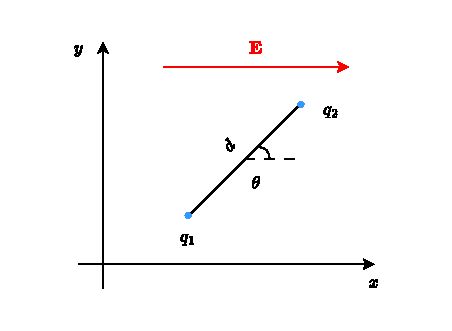
\includegraphics[width=0.5\linewidth]{res/svg/dipole.drawio}
\end{figure}
Now let us take a system made of two charges $q_1$ and $q_2$ of equal mass, with a bar with negligible mass that fixes the distance $d$. Imagine there is an electrostatic field acting on the particles. The motion of the particles is happening on a plane so we have 3 generalized coordinates. We can take the coordinates of the centre of mass $(X, Y)$ and the angle of the bar. We can split the contribution of the kinetic energy with the contribution of the centre of mass and the rotation around the centre of mass:
\begin{equation}
  T = T_{CM} + T' = \dfrac{1}{2}M(\dot{X}^2+\dot{Y}^2) + \dfrac{1}{2}I\dot{\theta}^2
\end{equation}
Now we know $M = 2m$ and $I = 2m\brackets{\dfrac{d}{2}}^2 = \dfrac{1}{2}md^2$. The kinetic energy is thus:
\begin{equation}
  T = m(\dot{X}^2+\dot{Y}^2) + \dfrac{1}{4}md^2\dot{\theta}^2
\end{equation}
Now we could in theory use three different approaches:
\begin{itemize}
  \item Use Lagrange equations
  \item Define a potential and use \eleref
  \item Find the Hamiltonian and use \hamiltonref
\end{itemize}
In this case we use the third method under the assumption that $\vec{E} = (E(x), 0, 0)$. Thus, the electric field is only given by the x component of a potential:
\begin{equation}
  E(x) = -\pdv{\potE}{x}
\end{equation}
The gravitational potential is negligible and so:
\begin{equation}
  V = q_1\potE(x_1) + q_2\potE(x_2)
\end{equation}
Which expressed in terms of the generalized coordinates becomes:
\begin{equation}
  V = q_1\potE \brackets{X - \dfrac{d}{2}\cos\theta} + q_2\potE \brackets{X + \dfrac{d}{2}\cos\theta}
\end{equation}
The Lagrangian is:
\begin{equation}
  \lagr = T - V = m(\dot{X}^2+\dot{Y}^2) + \dfrac{1}{4}md^2\dot{\theta}^2 - q_1\potE \brackets{X - \dfrac{d}{2}\cos\theta} - q_2\potE \brackets{X + \dfrac{d}{2}\cos\theta}
\end{equation}
We should also account for a interaction potential but since the distance is fixed this term would be constant and thus the Lagrangian can be defined without it. The Lagrangian does not depend on time thus:
\begin{equation}
  \pdv{\hamfun}{t} = - \pdv{\lagr}{t} = 0 \implies \dv{\hamfun}{t} = 0
\end{equation}
And so the Hamiltonian is a constant of the motion. Also transformation equations do not depend on time and the potential does not depend on the velocities thus $\hamfun = E$. So the Hamiltonian is the energy and it is conserved. Now we find the conjugated momenta:
\begin{equation}
  \begin{split}
    &p_X = \pdv{\lagr}{\dot{X}} = 2m\dot{X} \\[8pt]
    &p_Y = \pdv{\lagr}{\dot{Y}} = 2m\dot{Y} \\[8pt]
    &p_\theta = \pdv{\lagr}{\dot{\theta}} = \dfrac{1}{2}md^2\dot{\theta} = L_z \\[8pt]
  \end{split}
\end{equation}
The Hamiltonian will be:
\begin{equation}
  \begin{split}
    \hamfun &= 2m\dot{X}^2 + 2m\dot{Y}^2+ \dfrac{1}{2}md^2\dot{\theta}^2 - m(\dot{X}^2+\dot{Y}^2) - \dfrac{1}{4}md^2\dot{\theta}^2 + \\[8pt]
    &+ q_1\potE \brackets{X - \dfrac{d}{2}\cos\theta} + q_2\potE \brackets{X + \dfrac{d}{2}\cos\theta} = \\[8pt]
    &= m\brackets{\dot{X}^2 + \dot{Y}^2} + \dfrac{L_z^2}{md^2} + q_1\potE \brackets{X - \dfrac{d}{2}\cos\theta} + q_2\potE \brackets{X + \dfrac{d}{2}\cos\theta}
  \end{split}
\end{equation}
Now the interesting \hamiltonref\;are the ones who give the $\dot{p}_{\alpha}$ since we already know the $\dot{q}_{\alpha}$ in terms of the momenta from the Lagrangian part. We have that:
\begin{equation}
  \begin{split}
    &\dot{p}_X = -\pdv{\hamfun}{X} = - q_1 \pdv{\potE}{X} - q_2 \pdv{\potE}{X} = q_1E(x_1) + q_2E(x_2) \\[8pt]
    &\dot{p}_Y = -\pdv{\hamfun}{Y} = 0 \\[8pt]
    &\dot{p}_\theta = -\pdv{\hamfun}{\theta} = - q_1 \pdv{\potE}{\theta} - q_2 \pdv{\potE}{\theta} = - q_1 \pdv{\potE}{x_1}\pdv{x_1}{\theta} - q_2 \pdv{\potE}{x_2}\pdv{x_2}{\theta} = \\[8pt]
    &= q_1E(x_1)\dfrac{d}{2}\sin \theta - q_2E(x_2)\dfrac{d}{2}\sin \theta
  \end{split}
\end{equation}
And so $\dot{p}_X$ is the total force and $\dot{p}_{\theta}$ is the total torque. Now consider the case where the two charges are equal but have opposite sign ($q_1 = -q$, $q_2 = q$):
\begin{equation}
  \dot{p}_X = q \brackets{E(x_2) - E(x_1)}\\[8pt]
\end{equation}
If the field is uniform $E(x_2) = E(x_1) = E \implies \vec{F} = 0$, but we still have torque:
\begin{equation}
  \dv{L_z}{t} = -q\dfrac{d}{2}\sin \theta \brackets{E(x_1) + E(x_2)} = -\underbrace{qd}_p E\sin \theta
\end{equation}
And so:
\begin{equation}
  \dv{L_z}{t} = -\brackets{\vec{p} \cross \vec{E}}_z
\end{equation}
Where $\vec{p}$ is the dipole vector.
\subsection{Ex. 4}
\begin{figure}[H]
  \centering
  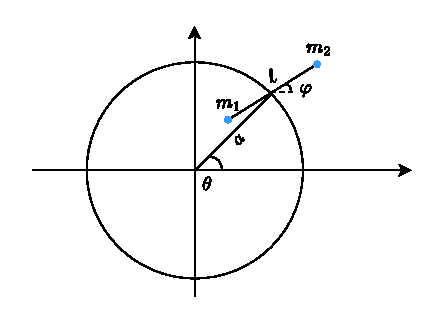
\includegraphics[width=0.7\linewidth]{res/svg/rail_and_bar.drawio}
\end{figure}
A massless bar of length $\ell$ with two bodies $m_1$, $m_2$ is attached in the centre of mass to a system composed of a vertical rail of radius $a$. The system is under the action of the gravitational potential. We have $2$ masses so we start from $3N = 6$ cartesian coordinates, but the motion is constrained on the vertical plane and we also have two constraints which are the bar and the rail so the number of independent coordinates is $n=2$. We can simply use the angles $\theta$ and $\varphi$ to describe the system. The coordiantes of the centre of mass are:
\begin{equation}
  \begin{split}
    X &= a\cos\theta \\[8pt]
    Y &= a\sin\theta
  \end{split}
\end{equation}
If the masses are equal $m_1 = m_2 = m$ then their coordiantes are:
\begin{equation}
  \begin{split}
    &x_1 = X - \dfrac{\ell}{2}\cos\varphi = a\cos\theta - \dfrac{\ell}{2}\cos\varphi \\[8pt]
    &y_1 = Y - \dfrac{\ell}{2}\sin\varphi = a\sin\theta - \dfrac{\ell}{2}\sin\varphi \\[8pt]
    &x_2 = X + \dfrac{\ell}{2}\cos\varphi = a\cos\theta + \dfrac{\ell}{2}\cos\varphi \\[8pt]
    &y_2 = Y + \dfrac{\ell}{2}\sin\varphi = a\sin\theta + \dfrac{\ell}{2}\sin\varphi \\[8pt]
  \end{split}
\end{equation}
The transformation equations do not depend on time so the kinetic energy will be a quadratic function of the velocities. We have that:
\begin{equation}
  \begin{split}
    &\dot{x}_1 = -a\dot{\theta}\sin\theta + \dfrac{\ell}{2}\dot{\varphi}\sin\varphi \\[8pt]
    &\dot{y}_1 = a\dot{\theta}\cos\theta - \dfrac{\ell}{2}\dot{\varphi}\cos\varphi \\[8pt]
    &\dot{x}_2 = -a\dot{\theta}\sin\theta - \dfrac{\ell}{2}\dot{\varphi}\sin\varphi \\[8pt]
    &\dot{y}_2 = a\dot{\theta}\cos\theta + \dfrac{\ell}{2}\dot{\varphi}\cos\varphi \\[8pt]
  \end{split}
\end{equation}
And so the kinetic energy will be:
\begin{equation}
  T = \frac{1}{2}m\left(\dot{x}_1^2 + \dot{y}_1^2 + \dot{x}_2^2 + \dot{y}_2^2\right) = m a^2 \dot{\theta}^2 + \frac{1}{4} m \ell^2 \dot{\varphi}^2
\end{equation}
We could have gotten this just by applying König's theorem:
\begin{equation}
  T = T' + T_{CM} = m a^2 \dot{\theta}^2 + \frac{1}{4} m \ell^2 \dot{\varphi}^2
\end{equation}
The potential is simply:
\begin{equation}
  V = mg\brackets{y_1 + y_2} = mg\brackets{a\sin\theta - \cancel{\dfrac{\ell}{2}\sin\varphi} + a\sin\theta + \cancel{\dfrac{\ell}{2}\sin\varphi}} = 2mga\sin\theta
\end{equation}
And so the Lagrangian is:
\begin{equation}
  \lagr = T - V = m a^2 \dot{\theta}^2 + \frac{1}{4} m \ell^2 \dot{\varphi}^2 - 2mga\sin\theta
\end{equation}
Thus the two conjugate momenta are:
\begin{equation}
  \begin{split}
    p_{\theta} = \pdv{\lagr}{\dot{\theta}} = 2m a^2 \dot{\theta} \\[8pt]
    p_{\varphi} = \pdv{\lagr}{\dot{\varphi}} = \dfrac{1}{2} m \ell^2 \dot{\varphi}
  \end{split}
\end{equation}
We can notice that $p_{\varphi}$ is constant since $\varphi$ is a cyclic coordinate. We can now find the Hamiltonian:
\begin{equation}
  \hamfun = p_{\theta}\dot{\theta} + p_{\varphi}\dot{\varphi} - \lagr = \frac{p_{\theta}^2}{4ma^2} + \frac{p_{\varphi}^2}{m\ell^2} + 2mga\sin\theta
\end{equation}
We only need to solve one Hamilton equation since we already know the relations between the coordinates and the momenta and we also knwo that $\dot{p}_{\varphi} = 0$ so we have:
\begin{equation}
  \dot{p}_{\theta} = -\pdv{\hamfun}{\theta} = -2mga\cos\theta
\end{equation}
The quantity $2mga\cos\theta$ is actually the $z$ component of the torque $\tau_z$ and this means that the system is rotating without a constant angular momentum under the action of gravity, which is what we expect from the setup we have. The equation above also gives us:
\begin{equation}
  \begin{split}
    &2m a^2 \ddot{\theta} = -2mga\cos\theta \\[8pt]
    &\ddot{\theta} + \dfrac{g}{a}\cos\theta = 0
  \end{split}
\end{equation}
\begin{figure}[H]
  \centering
  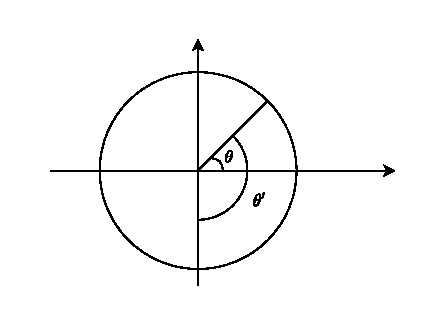
\includegraphics[width=0.5\linewidth]{res/svg/theta_prime.drawio}
\end{figure}
Now if we use the angle $\theta' = \theta + \dfrac{\pi}{2}$ to describe the system we end up with:
\begin{equation}
  \ddot{\theta'} + \dfrac{g}{a}\sin\theta' = 0
\end{equation}
Which is the equation of motion of a pendulum, so the bar is rotating with constant angular momentum around the centre of mass and the centre of mass is moving periodically on the rail.

\chapter{Applications of Lagrange formalism}
In this chapter we will discuss some potential applications of the Lagrange picture of classical mechanics.
\section{Theory of small oscillations}
Many physical problems have an oscillatory nature but, when we try to solve those problems, we usually encounter difficult (sometimes impossible) differential equations.
For this reason we now introduce a systematic way to deal with oscillatory problems in the case of a small oscillation.
\subsection{$\mathbf{n = 1}$ degree of freedom systems}
Let's start with a 1 degree of freedom system. In this case the Lagrangian may look something like this:
\begin{equation}
    \lagr = \dfrac{1}{2}m\dot{q}^2 - V(q)
\end{equation}
Notice that we asked for a potential that only depends on the coordinate $q$.
We take in consideration the system near point of local minimum for the potential.
\begin{figure}[!ht]
    \centering
    \includesvg[width=0.6\textwidth]{res/svg/potential1Dapprox}
    \caption{1-D potential}
    \label{fig:image10}
\end{figure}
Given this we can approximate the potential to it's second order Taylor expansion near the point $q_0$ (local minimum):
\begin{equation}
    V \simeq V(q_0) + \cancel{\pdv{V}{q}\bigg|_{q_0}}(q-q_0) + \dfrac{1}{2}\pdv[2]{V}{q}\bigg|_{q_0}(q-q_0)^2
\end{equation}
The first derivative is zero since we are at a minimum, we can also ignore the value of the potential $V(q_0)$ and set it equal to zero, since we can always change the potential reference. Finally, we define:
\begin{equation}
    \eta \defineeq q-q_0
\end{equation}
And so we get:
\begin{equation} \label{e:potential_1D_oscillation}
    V(\eta) \simeq \dfrac{1}{2}\underbrace{\pdv[2]{V}{\eta}\bigg|_{q_0}}_{\Velegant}\eta^2 = \dfrac{1}{2}\Velegant\eta^2
\end{equation}
Where we defined the second order partial derivative as a known quantity $\Velegant$. We also know that, since $q$ and $\eta$ are different only for a constant term:
\begin{equation} \label{e:kinetic_1D_oscillation}
    T = \dfrac{1}{2}m\dot{q}^2 = \dfrac{1}{2}m\dot{\eta}^2
\end{equation}
From this we can write the \eleref :
\begin{equation}
    \begin{split}
        \dv{}{t}\pdv{\lagr}{\dot{\eta}} -\pdv{\lagr}{\eta} = 0 \\[8pt]
        \dv{}{t}\pdv{T}{\dot{\eta}} + \pdv{V}{\eta} = 0
    \end{split}
\end{equation}
Substituting what we got in \eqref{e:potential_1D_oscillation} and \eqref{e:kinetic_1D_oscillation}:
\begin{equation}
    \begin{split}
        \dv{}{t}(m\dot{\eta}) + \Velegant\eta &= 0\\[8pt]
        m\ddot{\eta} + \Velegant\eta &= 0
    \end{split}
\end{equation}
From which we get this condition:
\begin{equation} \label{e:condition_1D_oscillation}
    \ddot{\eta} =- \dfrac{\Velegant\eta}{m}
\end{equation}
We are searching for solutions of this type:
\begin{equation}
    \eta (t) = a\efunction^{-i\omega t}
\end{equation}
And so we evaluate the second order derivative:
\begin{eqnarray}
    \ddot{\eta} (t) = -a\omega^2\efunction^{-i\omega t}
\end{eqnarray}
We now impose the condition that $a\neq 0$ which is reasonable since $a=0$ would correspond to the absence of motion, so from \eqref{e:condition_1D_oscillation} we get:
\begin{equation}
    \begin{split}
        m\omega^2\cancel{a\efunction^{-i\omega t}} &= \Velegant\cancel{a\efunction^{-i\omega t}}\\[8pt]
        \omega &= \pm \sqrt{\dfrac{\Velegant}{m}}
    \end{split}
\end{equation}
By convention we usually take the $+$ sign and refer to the other solution as $-\omega$. The general solution for $\eta$ will be of this form:
\begin{equation}
    \eta (t) = ca\efunction^{-i\omega t} + c'a\efunction^{i\omega t} = A \sin(\omega t + \varphi) = A \sin\brackets{\sqrt{\dfrac{\Velegant}{m}} t + \varphi}
\end{equation}
\subsection{$\mathbf{n\geq 2}$ degrees of freedom systems}
Now we want to discuss a more general type of system with $n\geq2$ degrees of freedom. Again we take in consideration a point $\vec{q}_0 = (q_{1,0}, q_{2,0}, \,\dots\, ,q_{n,0})$ of local minimum for the potential $V$ which now is a function of all the coordinates $q_{\alpha}$.
\begin{figure}[!ht]
    \centering
    \includesvg[width=0.6\textwidth]{res/svg/potential2Dapprox}
    \caption{2-D potential}
    \label{fig:image11}
\end{figure}
In this case the potential can be approximated near the point with the Taylor formula for multivariable scalar functions:
\begin{equation} \label{e:taylor_potential_scalar_product}
    V(\vec{q}) \simeq \underbrace{V(\vec{q}_0)}_{\text{constant}} + \cancel{\langle \grad V(\vec{q}_0), \vec{q}-\vec{q}_0\rangle} + \dfrac{1}{2}\langle H V(\vec{q}_0)(\vec{q}-\vec{q}_0), (\vec{q}-\vec{q}_0)\rangle
\end{equation}
Again we exploit the fact that we can choose an arbitrary level for the potential, and we define:
\begin{equation}
    \eta_{\alpha} = q_{\alpha} - q_{\alpha,0}
\end{equation}
Expanding \eqref{e:taylor_potential_scalar_product} we get:
\begin{equation}
    \begin{split}
        V(\vec{q}) &\simeq \dfrac{1}{2}\bigsum_{\alpha}\bigsum_{\beta}\dfrac{\partial^2 V}{\partial q_{\alpha} \partial q_{\beta}}\bigg|_{\vec{0}}(q_{\alpha} - q_{\alpha,0})(q_{\beta} - q_{\beta,0})\\[8pt]
        V(\vec{\eta}) &\simeq \dfrac{1}{2}\bigsum_{\alpha}\bigsum_{\beta}\underbrace{\dfrac{\partial^2 V}{\partial \eta_{\alpha} \partial \eta_{\beta}}\bigg|_{\vec{0}}}_{\Velegant_{\alpha \beta} = \Velegant_{\beta \alpha}}\eta_{\alpha}\eta_{\beta}\\[8pt]
        V(\vec{\eta}) &\simeq \dfrac{1}{2}\bigsum_{\alpha}\bigsum_{\beta}\Velegant_{\alpha \beta}\eta_{\alpha}\eta_{\beta}
    \end{split}
\end{equation}
For the kinetic energy $T$ we assume that the transformation equations do not depend on time:
\begin{equation}
    T = \dfrac{1}{2}\bigsum_{\alpha}\bigsum_{\beta}\Telegant'_{\alpha \beta} \dot{\eta}_{\alpha}\dot{\eta}_{\beta}
\end{equation}
We consider the Taylor expansion of $\Telegant'_{\alpha \beta}$. In this case we can stop at the first order because there is no reason to assume that the kinetic energy and the potential energy have a minimum at the same point:
\begin{equation}
    \Telegant'_{\alpha \beta} \simeq \Telegant'_{\alpha \beta}(\vec{0}) + \bigsum_{\gamma}\pdv{\Telegant'_{\alpha \beta}}{\eta_{\gamma}}\bigg|_{\vec{0}}\eta_{\gamma}
\end{equation}
Going back to the general expression for $T$ we get:
\begin{equation}
    \begin{split}
        T &\simeq \dfrac{1}{2}\bigsum_{\alpha}\bigsum_{\beta}\brackets{\Telegant'_{\alpha \beta}(\vec{0}) + \bigsum_{\gamma}\pdv{\Telegant'_{\alpha \beta}}{\eta_{\gamma}}\bigg|_{\vec{0}}\eta_{\gamma}} \dot{\eta}_{\alpha}\dot{\eta}_{\beta} =\\[8pt]
        &= \dfrac{1}{2}\bigsum_{\alpha}\bigsum_{\beta}\bigsum_{\gamma}\underbrace{\pdv{\Telegant'_{\alpha \beta}}{\eta_{\gamma}}\bigg|_{\vec{0}}\eta_{\gamma} \dot{\eta}_{\alpha}\dot{\eta}_{\beta}}_{o(\eta \dot{\eta}^2)} + \dfrac{1}{2}\bigsum_{\alpha}\bigsum_{\beta}\underbrace{\Telegant'_{\alpha \beta}(\vec{0})\dot{\eta}_{\alpha}\dot{\eta}_{\beta}}_{o(\dot{\eta}^2)}
    \end{split}
\end{equation}
We can neglect the first term since it is small with respect to the second term. Now we define:
\begin{equation}
    \Telegant_{\alpha \beta} \defineeq \Telegant'_{\alpha \beta}(\vec{0})
\end{equation}
Those are just numbers which correspond to the value of the kinetic energy at the origin. We can put those numbers into a matrix:
\begin{equation}
    \hat{\Telegant}=
    \begin{pmatrix}
        \Telegant_{1 1} & \Telegant_{1 2} &  \,\dots\,  & \Telegant_{1 n}\\[8pt]
        \Telegant_{2 1} & \Telegant_{2 2} &  \,\dots\,  &  \,\dots\, \\[8pt]
         \,\dots\,  &  \,\dots\,  &  \,\dots\,  &  \,\dots\, \\[8pt]
        \Telegant_{n 1} &  \,\dots\,  &  \,\dots\,  & \Telegant_{n n}\\[8pt]
    \end{pmatrix}
\end{equation}
Similarly we can put the values of $\Velegant_{\alpha \beta}$ into a matrix:
\begin{equation}
    \hat{\Velegant}=
    \begin{pmatrix}
        \Velegant_{1 1} & \Velegant_{1 2} &  \,\dots\,  & \Velegant_{1 n}\\[8pt]
        \Velegant_{2 1} & \Velegant_{2 2} &  \,\dots\,  &  \,\dots\, \\[8pt]
         \,\dots\,  &  \,\dots\,  &  \,\dots\,  &  \,\dots\, \\[8pt]
        \Velegant_{n 1} &  \,\dots\,  &  \,\dots\,  & \Velegant_{n n}\\[8pt]
    \end{pmatrix}
\end{equation}
Also we have that:
\begin{equation}
    \dfrac{1}{2}\bigsum_{\alpha}\bigsum_{\beta}\Telegant_{\alpha \beta}\dot{\eta}_{\alpha}\dot{\eta}_{\beta}
\end{equation}
So the Lagrangian for the system is:
\begin{equation}
    \lagr = \dfrac{1}{2}\bigsum_{\alpha}\bigsum_{\beta}\brackets{\Telegant_{\alpha \beta}\dot{\eta}_{\alpha}\dot{\eta}_{\beta} - \Velegant_{\alpha \beta}\eta_{\alpha}\eta_{\beta}}
\end{equation}
The terms of the \eleref\;are:
\begin{equation}
    \begin{split}
        \pdv{\lagr}{\eta_{\gamma}} &= -\pdv{V}{\eta_{\gamma}} = -\dfrac{1}{2}\bigsum_{\alpha}\bigsum_{\beta}\Velegant_{\alpha \beta} \pdv{}{\eta_{\gamma}}\brackets{\eta_{\alpha}\eta_{\beta}}\\[8pt]
        \pdv{\lagr}{\dot{\eta}_{\gamma}} &= \pdv{T}{\dot{\eta}_{\gamma}} = \dfrac{1}{2}\bigsum_{\alpha}\bigsum_{\beta}\Telegant_{\alpha \beta}\pdv{}{\dot{\eta}_{\gamma}}\brackets{\dot{\eta}_{\alpha}\dot{\eta}_{\beta}}
    \end{split}
\end{equation}
Evaluating the partial derivatives we get:
\begin{equation}
    \begin{split}
        \pdv{\lagr}{\eta_{\gamma}} &= -\dfrac{1}{2}\bigsum_{\alpha}\bigsum_{\beta}\Velegant_{\alpha \beta} \bbrackets{\eta_{\beta}\underbrace{\pdv{\eta_{\alpha}}{\eta_{\gamma}}}_{\delta_{\gamma \alpha}} + \eta_{\alpha}\underbrace{\pdv{\eta_{\beta}}{\eta_{\gamma}}}_{\delta_{\gamma \beta}}} =\\[8pt]
        &= -\dfrac{1}{2}\bigsum_{\alpha}\bigsum_{\beta}\Velegant_{\alpha \beta} \eta_{\beta}\delta_{\gamma \alpha} - \dfrac{1}{2}\bigsum_{\alpha}\bigsum_{\beta}\Velegant_{\alpha \beta} \eta_{\alpha}\delta_{\gamma \beta} = \\[8pt]
        &= -\dfrac{1}{2}\bigsum_{\beta}\Velegant_{\gamma \beta} \eta_{\beta} - \dfrac{1}{2}\bigsum_{\alpha}\Velegant_{\alpha \gamma} \eta_{\alpha} =\\[8pt]
        &= -\bigsum_{\alpha}\Velegant_{\alpha \gamma} \eta_{\alpha}
    \end{split}
\end{equation}
We simplified the summation in the second line because of the Kronecker delta, and we can notice that in the third line the two terms are actually identical due to the fact that $\Velegant_{\alpha \gamma} = \Velegant_{\gamma \beta}$ and we are summing over all indices. The calculation for the kinetic energy is the same, and we get:
\begin{equation}
    \pdv{\lagr}{\dot{\eta}_{\gamma}} = \bigsum_{\alpha}\Telegant_{\alpha \gamma} \dot{\eta}_{\alpha}
\end{equation}
Hence we evaluate the total time derivative:
\begin{equation}
    \dv{}{t}\pdv{\lagr}{\dot{\eta}_{\gamma}} = \dv{}{t}\bigsum_{\alpha}\Telegant_{\alpha \gamma} \eta_{\alpha} = \bigsum_{\alpha}\Telegant_{\alpha \gamma} \ddot{\eta}_{\alpha}
\end{equation}
So the \eleref\;are:
\begin{equation} \label{e:ele_for_gamma}
    \bigsum_{\alpha}\brackets{\Telegant_{\alpha \gamma} \ddot{\eta}_{\alpha} + \Velegant_{\alpha \gamma} \eta_{\alpha}} = 0
\end{equation}
for all the possible $\gamma$.\\
Taking into account the fact that we look for solutions like:
\begin{equation}
    \eta_{\alpha} (t) = a_{\alpha}\efunction^{-i\omega t}
\end{equation}
\textbf{N.B.} The coefficients $a_{\alpha}$ may be complex numbers.\\
Substituting into \eqref{e:ele_for_gamma} we get:
\begin{equation} \label{e:eigenvalue_alpha}
    \begin{split}
        \bigsum_{\alpha}\brackets{-\omega^2\Telegant_{\alpha \gamma} a_{\alpha}\cancel{\efunction^{-i\omega t}} + \Velegant_{\alpha \gamma}a_{\alpha}\cancel{\efunction^{-i\omega t}}} &= 0\\[8pt]
        \bigsum_{\alpha}\brackets{-\omega^2\Telegant_{\alpha \gamma} + \Velegant_{\alpha \gamma}}a_{\alpha} &= 0
    \end{split}
\end{equation}
This is true for any $\gamma$ so we are obtaining a set of \textit{homogeneous first order equations}. We know from linear algebra that the only way for this system to allow solutions different from the trivial solution is to ask for at least one equation to be a linear combination of the others.
In other terms we want the determinant of the coefficient matrix to be zero. We can now express the system as follows:
\begin{equation}
    \brackets{-\omega^2\hat{\Telegant} + \hat{\Velegant}}\vec{a} = \vec{0}
\end{equation}
Let $\lambda = \omega^2$:
\begin{equation}
    \boxed{\hat{\Velegant}\vec{a} = \lambda\hat{\Telegant}\vec{a}}
\end{equation}
This equation is called \textbf{generalized eigenvalue equation}. In fact if we have $\hat{\Telegant} = \mathbb{I}$ we return to the ``regular'' eigenvalue equation. In order to find the coefficients $\lambda$ we must solve this equation:
\begin{equation}
    \det(\hat{\Velegant}-\lambda\hat{\Telegant}) = 0
\end{equation}
This is an $n$ degree polynomial with $n$ solutions $\lambda_i$ with $i=1,2, \,\dots\, ,n$. The solutions satisfy some properties:
\begin{itemize}
    \item $\lambda_i \in \mathbb{R}$
    \item $\lambda_i > 0$
\end{itemize}
This means that $\omega_i = \pm \sqrt{\lambda_i}$ is real for any $i$. Putting $\lambda_i$ back into \eqref{e:eigenvalue_alpha} we get an expression depending on $\gamma$, thus we have a system of equations:
\begin{equation}
    \begin{cases}
        \bigsum_{\alpha}\brackets{-\lambda_i\Telegant_{\alpha 1} + \Velegant_{\alpha 1}}a_{\alpha}^{(i)} &= 0\\[10pt]
        \bigsum_{\alpha}\brackets{-\lambda_i\Telegant_{\alpha 2} + \Velegant_{\alpha 2}}a_{\alpha}^{(i)} &= 0\\[10pt]
         \,\dots\, \\[10pt]
        \bigsum_{\alpha}\brackets{-\lambda_i\Telegant_{\alpha n} + \Velegant_{\alpha n}}a_{\alpha}^{(i)} &= 0
    \end{cases}
\end{equation}
In this system at least one equation is linearly dependent on the others since we asked that the determinant of the coefficient matrix is zero. In this way we can find all the components of the vector $\vec{a}^{(i)}$, which is called \textbf{generalized eigenvector}.
Those vectors must satisfy a condition:
\begin{equation}
    [\vec{a}^{(i)}]^{\dagger}\;\hat{\Telegant}\;[\vec{a}^{(j)}] = 0
\end{equation}
This condition is called $\hat{\Telegant}$-orthogonality and is a generalization of the concept of orthogonality. In fact this condition reduces to the ``usual'' case if $\hat{\Telegant} = \mathbb{I}$ and the vectors are real valued:
\begin{equation}
    \begin{split}
        [\vec{a}^{(i)}]^{\dagger}\;\mathbb{I}\;[\vec{a}^{(j)}] &= 0\\[8pt]
        \transpose{[\vec{a}^{(i)}]} [\vec{a}^{(j)}] &= 0 \\[8pt]
        \vec{a}^{(i)}\cdot \vec{a}^{(j)} &= 0
    \end{split}
\end{equation}
We also want to normalize the vectors. Again the concept of normalization is generalized as follows:
\begin{equation}
    [\vec{a}^{(i)}]^{\dagger}\;\hat{\Telegant}\;[\vec{a}^{(i)}] = 1
\end{equation}
A solution to the system is:
\begin{equation}
    \vec{\eta} = \begin{pmatrix}
        \eta_1\\[8pt]
        \eta_2\\[8pt]
         \,\dots\, \\[8pt]
        \eta_n
    \end{pmatrix}
    =
    \begin{pmatrix}
        a_1\\[8pt]
        a_2\\[8pt]
         \,\dots\, \\[8pt]
        a_n
    \end{pmatrix}\efunction^{-i\omega t}
\end{equation}
Actually a more general solution is given by a linear combination of this solution:
\begin{equation}
    \begin{split}
        \vec{\eta} &= \bigsum_i\brackets{c_i \vec{a}^{(i)} \efunction^{-i\omega_i t} + c_i' \vec{a}^{(i)} \efunction^{i\omega_i t}} =\\[8pt]
        &= \bigsum_i \underbrace{\brackets{c_i \efunction^{-i\omega_i t} + c_i' \efunction^{i\omega_i t}}}_{\text{components of $\vec{\eta}$ along $\vec{a}^{(i)}$}}\vec{a}^{(i)}
    \end{split}
\end{equation}
For each component we have:
\begin{equation}
    \begin{split}
        \eta_{\alpha} &= \bigsum_i \brackets{c_i \efunction^{-i\omega_i t} + c_i' \efunction^{i\omega_i t}}a_{\alpha}^{(i)} =\\[8pt]
        &=  \underbrace{\bigsum_i A_i \sin(\omega_i t + \varphi_i)}_{\text{non monochromatic}}
    \end{split}
\end{equation}
The terms $\omega_i$ are called \textbf{normal mode frequencies}, and generally they are all different.\\
It is possible to express the solutions as pure harmonic motions (monochromatic) if one uses the eigenvectors as basis vectors. We can also notice that both $\hat{\Velegant}$ and $\hat{\Telegant}$ are diagonalized by the eigenvectors $\vec{a}^{(i)}$.
In this base solution is in the form:
\begin{equation}
    u_i = A_i \sin(\omega_i t + \varphi_i)
\end{equation}
Which indeed is monochromatic. Writing the \eleref\;in this basis we have:
\begin{equation}
    \ddot{u}_i +\lambda_i u_i = 0 \;\;\forall i=1, \,\dots\, ,n
\end{equation}
\subsection{2-D systems. General example}
Let's assume we are dealing with a two-dimensional system with a minimum for the potential at $(q_{10},q_{20})$. Also assume that the kinetic energy taxes the form of:
\begin{equation}
    \hat{\Telegant} = m\begin{pmatrix}
        1 & 0\\[8pt]
        0 & 1
    \end{pmatrix} \Rightarrow \Telegant_{\alpha \beta} = m\delta_{\alpha \beta}
\end{equation}
Expanding the potential in terms of $\eta_1 = q_1-q_{10}$ and $\eta_2 = q_2-q_{20}$ gives:
\begin{equation}
    \begin{split}
        V &\simeq \dfrac{1}{2}\bigsum_{\alpha}\bigsum_{\beta}\brackets{\dfrac{\partial^2 V}{\partial \eta_{\alpha} \partial \eta_{\beta}}\bigg|_{(0,0)}\eta_{\alpha}\eta_{\beta}} =\\[8pt]
        &= \dfrac{1}{2}(\Velegant_{11}\eta_1^2 + \Velegant_{22}\eta_2^2 + \underbrace{\Velegant_{12}\eta_1\eta_2 + \Velegant_{21}\eta_2\eta_1}_{\text{same term}}) =\\[8pt]
        &= \dfrac{1}{2}(\Velegant_{11}\eta_1^2 + \Velegant_{22}\eta_2^2 + 2\Velegant_{12}\eta_1\eta_2 )
    \end{split}
\end{equation}
The kinetic energy instead becomes:
\begin{equation}
    \begin{split}
        T &= \dfrac{1}{2}\bigsum_{\alpha}\bigsum_{\beta}m \delta_{\alpha \beta} \dot{\eta}_{\alpha}\dot{\eta}_{\beta} =\\[8pt]
        &= \dfrac{1}{2}m(\dot{\eta}_1^2 + \dot{\eta}_2^2)
    \end{split}
\end{equation}
The Lagrangian then becomes:
\begin{equation}
    \lagr = \dfrac{1}{2}m(\dot{\eta}_1^2 + \dot{\eta}_2^2) - \dfrac{1}{2}(\Velegant_{11}\eta_1^2 + \Velegant_{22}\eta_2^2 + 2\Velegant_{12}\eta_1\eta_2 )
\end{equation}
Let us divide the Lagrangian by $m$ and define:
\begin{equation}
    \lagr' = \dfrac{1}{m}\lagr
\end{equation}
\begin{equation}
    \hat{\Telegant}' = \dfrac{1}{m}\hat{\Telegant} = \begin{pmatrix}
        1 & 0\\[8pt]
        0 & 1
    \end{pmatrix}
\end{equation}
\begin{equation}
    \hat{\Velegant}' = \dfrac{1}{m}\hat{\Velegant} = \begin{pmatrix}
        \dfrac{\Velegant_{11}}{m} & \dfrac{\Velegant_{12}}{m}\\[8pt]
        \dfrac{\Velegant_{21}}{m} & \dfrac{\Velegant_{22}}{m}
    \end{pmatrix} = \begin{pmatrix}
        \Velegant_{11}' & \Velegant_{12}'\\[8pt]
        \Velegant_{21}' & \Velegant_{22}'
    \end{pmatrix}
\end{equation}
The new Lagrangian becomes:
\begin{equation}
    \lagr' = \dfrac{1}{2}\transpose{\dvec{\eta}} \dvec{\eta} - \dfrac{1}{2}\transpose{\vec{\eta}} \Velegant' \vec{\eta}
\end{equation}
From \eleref\;we get two equations:
\begin{equation}
    \begin{cases}
        \ddot{\eta}_1 + \Velegant'_{11}\eta_1 + \Velegant'_{12}\eta_2 = 0\\[8pt]
        \ddot{\eta}_2 + \Velegant'_{22}\eta_2 + \Velegant'_{12}\eta_1 = 0
    \end{cases} \bigg|\;\text{coupled equations}
\end{equation}
Now impose that the solutions are in the form:
\begin{equation}
    \begin{split}
        \eta_1 = a_1\efunction^{-i\omega t} \\[8pt]
        \eta_2 = a_2\efunction^{-i\omega t}
    \end{split}
\end{equation}
The system becomes:
\begin{equation}
    \begin{cases}
        -\omega^2 a_1 + \Velegant'_{11}a_1 + \Velegant'_{12}a_2 = 0\\[8pt]
        \Velegant'_{12}a_1 -\omega^2 a_2 + \Velegant'_{22}a_2 = 0
    \end{cases}
\end{equation}
In this case the generalized eigenvalue equation reduces to the usual case, and we get the two solutions $\lambda_1$ and $\lambda_2$. Substituting $\lambda_1$ into the eigenvalue equation we get:
\begin{equation}
    \begin{cases}
        \brackets{\Velegant'_{11}-\lambda_1}a_1^{(1)} + \Velegant'_{12}a_2^{(1)} = 0\\[8pt]
        \Velegant'_{12}a_1^{(1)} + \brackets{\Velegant'_{22}-\lambda_1}a_2^{(1)} = 0
    \end{cases}
\end{equation}
One of the two equation must depend on the other. Since we have two equations we can arbitrarily pick one and get the relation between the coefficients:
\begin{equation}
    a_2^{(1)} = a_1^{(1)}\dfrac{\lambda_1 - \Velegant'_{11}}{\Velegant'_{12}}
\end{equation}
And so we have:
\begin{equation}
    \vec{a}^{\;(1)} = a_1^{(1)}\begin{pmatrix}
        1 \\[8pt] \dfrac{\lambda_1 - \Velegant'_{11}}{\Velegant'_{12}}
    \end{pmatrix}
\end{equation}
Similarly for $\lambda_2$ we get:
\begin{equation}
    \vec{a}^{\;(2)} = a_1^{(2)}\begin{pmatrix}
        1 \\[8pt] \dfrac{\lambda_2 - \Velegant'_{11}}{\Velegant'_{12}}
    \end{pmatrix}
\end{equation}
Now let's define:
\begin{equation}
    \begin{split}
        K_1\;\text{s.t.}\; a^{(1)} = K_1\Velegant'_{12}\\[8pt]
        K_2\;\text{s.t.}\; a^{(2)} = K_2\Velegant'_{12}
    \end{split}
\end{equation}
And the vectors can be rewritten as:
\begin{equation}
    \begin{split}
        \vec{a}^{\;(1)} = K_1\begin{pmatrix}
            \Velegant'_{12} \\[8pt] \lambda_1 - \Velegant'_{11}
        \end{pmatrix}\\[8pt]
        \vec{a}^{\;(2)} = K_2\begin{pmatrix}
            \Velegant'_{12} \\[8pt] \lambda_2 - \Velegant'_{11}
        \end{pmatrix}
    \end{split}
\end{equation}
The most general solution is a linear combination of all the single solutions:
\begin{equation}
    \vec{\eta} = \begin{pmatrix}
        c_1 a_1^{(1)}\efunction^{-i\omega_1 t} + c_1' a_1^{(1)}\efunction^{i\omega_1 t} + c_2 a_1^{(2)}\efunction^{-i\omega_2 t} + c_2' a_1^{(2)}\efunction^{i\omega_2 t}\\[8pt]
        c_1 a_2^{(1)}\efunction^{-i\omega_1 t} + c_1' a_2^{(1)}\efunction^{i\omega_1 t} + c_2 a_2^{(2)}\efunction^{-i\omega_2 t} + c_2' a_2^{(2)}\efunction^{i\omega_2 t}
    \end{pmatrix}
\end{equation}
Substituting the components of the vectors $\vec{a}$:
\begin{equation}
    \begin{split}
        \vec{\eta} = \begin{pmatrix}
            c_1 K_1\Velegant'_{12}\efunction^{-i\omega_1 t} + c_1' K_1\Velegant'_{12}\efunction^{i\omega_1 t} +  \,\dots\, \\[8pt]
            c_1 K_1\Velegant'_{12}\efunction^{-i\omega_1 t} + c_1' K_1\Velegant'_{12}\efunction^{i\omega_1 t} +  \,\dots\,
        \end{pmatrix}\\[8pt]
        \vec{\eta} = \begin{pmatrix}
            A_1 \sin(\omega_1 t + \varphi_1) + A_2 \sin(\omega_2 t + \varphi_2)\\[8pt]
            A_1 \sin(\omega_1 t + \varphi_1) + A_2 \sin(\omega_2 t + \varphi_2)
        \end{pmatrix}
    \end{split}
\end{equation}
But if we change basis we get:
\begin{equation}
    \vec{\eta} = u_1 \vec{a}^{\;(1)} + u_2 \vec{a}^{\;(2)}
\end{equation}
Where:
\begin{equation}
    \begin{split}
        u_1 = A_1 \sin(\omega_1 t + \varphi_1)\\[8pt]
        u_2 = A_2 \sin(\omega_2 t + \varphi_2)
    \end{split}
\end{equation}
Which are monochromatic signals. Also in this new basis we have:
\begin{equation}
    \begin{split}
        \hat{\Telegant}' = \begin{pmatrix}
            1 & 0\\[8pt]
            0 & 1
        \end{pmatrix}\\[8pt]
        \hat{\Velegant}' = \begin{pmatrix}
            \lambda_1 & 0\\[8pt]
            0 & \lambda_2
        \end{pmatrix}
    \end{split}
\end{equation}
And so the \eleref\;become:
\begin{equation}
    \begin{cases}
        \ddot{u}_1+\lambda_1 u_1 = 0\\[8pt]
        \ddot{u}_2+\lambda_2 u_2 = 0
    \end{cases}
\end{equation}
Those are not coupled equations, and so they can be solved separately.


\subsection{2-D systems. Coupled pendulums}
Now let's take a particular system composed of two ideal pendulums in which the masses are attached by a spring as shown:
\begin{figure}[!ht]
    \centering
    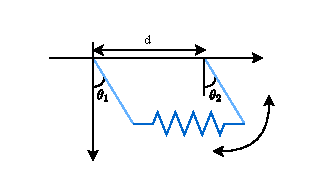
\includegraphics[width=0.6\textwidth]{res/svg/couple_pendulum_1.drawio}
    \caption{Coupled pendulums}
\end{figure}
The rest length of the spring is $d$. Since we have two particles, in principle we have at least $N=3\cdot2=6$ coordinates. Two coordinates can be neglected because the motion only occurs in the $xy$-plane.
The two ropes are a constraint on the position of the particles. In particular both constraints are holomonic and sclermonic:
\begin{equation}
    \begin{cases}
        x_1^2 + y_1^2 = l & \text{(first rope)}\\[8pt]
        (x_2-d)^2 + y_2^2 = l & \text{(second rope)}
    \end{cases}
\end{equation}
We can write the transformation equations as follows:
\begin{equation}
    \begin{cases}
        x_1 = l\sin\theta_1\\[8pt]
        y_1 = -l\cos\theta_1
    \end{cases}\;\;
    \begin{cases}
        x_2 = l\sin\theta_2+d\\[8pt]
        y_2 = -l\cos\theta_2
    \end{cases}
\end{equation}
Since transformation equations do not depend on time the kinetic energy will be a quadratic function of the velocities:
\begin{equation}
    \begin{split}
        T &= \dfrac{1}{2}m(\underbrace{\dot{x}_1^2+\dot{y}_1^2}_{(l\dot{\theta}_1)^2}) + \dfrac{1}{2}m(\underbrace{\dot{x}_2^2+\dot{y}_2^2}_{(l\dot{\theta}_2)^2}) \\[8pt]
        &= \dfrac{1}{2}ml^2(\dot{\theta}_1^2+\dot{\theta}_2^2)
    \end{split}
\end{equation}
We can express this in a matrix form as:
\begin{equation}
    \begin{split}
        T &= \dfrac{1}{2}(\dot{\theta}_1 \dot{\theta}_2)\hat{\Telegant}\begin{pmatrix}
            \dot{\theta}_1 \\[8pt]\dot{\theta}_2
        \end{pmatrix} = \\[8pt]
        &= \dfrac{1}{2}(\dot{\theta}_1 \dot{\theta}_2)ml^2\begin{pmatrix}
            1 & 0\\[8pt]
            0 & 1
        \end{pmatrix}
        \begin{pmatrix}
            \dot{\theta}_1 \\[8pt]\dot{\theta}_2
        \end{pmatrix} = \\[8pt]
    \end{split}
\end{equation}
The potential is the sum of the gravitational potentials of the masses and of the elastic potential of the spring:
\begin{equation}
    \begin{split}
        V &= \underbrace{mgy_1 + mgy_2}_{-mgl(\cos\theta_1+\cos\theta_1)} + \dfrac{1}{2}k\left[\sqrt{(x_2-x_1)^2+(y_2-y_1)^2}-d\right]^2\\[8pt]
        &= -mgl(\cos\theta_1+\cos\theta_1) +\\[8pt]
        &+ \dfrac{1}{2}k\left[\sqrt{(l\sin\theta_2+d-l\sin\theta_1)^2+(l\cos\theta_1-l\cos\theta_2)^2}-d\right]^2\\[8pt]
    \end{split}
\end{equation}
To find the minimum value of the potential we should theoretically evaluate the gradient and solve for $\grad V = \vec{0}$, but if we look at the configuration we can easily notice that the potential is minimum when the pendulums are in the vertical position and the spring is at rest as shown:
\begin{figure}[H]
    \centering
    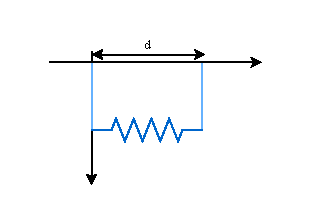
\includegraphics[width=0.6\textwidth]{res/svg/couple_pendulum_still.drawio}
\end{figure}
Thus we can expand the potential at $(0,0)$. Notice that the coordinates $\eta_1$ and $\eta_2$ in this case are equivalent to the ones we chose:
\begin{equation}
    \begin{split}
        V &\simeq V(0,0) +\dfrac{1}{2}\bigsum_{\alpha}\bigsum_{\beta} \dfrac{\partial^2 V}{\partial \theta_{\alpha} \partial \theta_{\beta}}\bigg|_{(0,0)}\theta_{\alpha}\theta_{\beta} = \\[8pt]
        &= V(0,0) +\dfrac{1}{2}\brackets{\Velegant_{11}\theta_1^2 + \Velegant_{22}\theta_2^2 + 2\Velegant_{12}\theta_1\theta_2}
    \end{split}
\end{equation}
This can be expressed in matrix form:
\begin{equation}
    \begin{split}
        V &= \dfrac{1}{2}(\theta_1\;\theta_2)\hat{\Velegant}\begin{pmatrix}
            \theta_1 \\[8pt]
            \theta_2
        \end{pmatrix}\\[8pt]
        V &= \dfrac{1}{2}(\theta_1\;\theta_2)\begin{pmatrix}
            \Velegant_{11} & \Velegant_{12}\\[8pt]
            \Velegant_{12} & \Velegant_{22}
        \end{pmatrix} \begin{pmatrix}
            \theta_1 \\[8pt]
            \theta_2
        \end{pmatrix}
    \end{split}
\end{equation}
If we evaluate all the partial derivatives we get that the matrix $\hat{\Velegant}$ is:
\begin{equation}
    \hat{\Velegant} = \begin{pmatrix}
        mgl+kl^2 & -kl^2\\[8pt]
        -kl^2 & mgl+kl^2
    \end{pmatrix}
\end{equation}
The Lagrangian finally looks like this:
\begin{equation}
    \lagr = \dfrac{1}{2}ml^2(\dot{\theta}_1^2+\dot{\theta}_2^2) - \dfrac{1}{2}\left[(mgl+kl^2)\theta_1^2 + 2(-kl^2)\theta_1\theta_2 + (mgl+kl^2)\theta_2^2 \right]
\end{equation}
And the \eleref\;are:
\begin{equation}
    \begin{cases}
        ml^2\ddot{\theta}_1 + (mgl + kl^2)\theta_1 - kl^2\theta_2 = 0\\[8pt]
        ml^2\ddot{\theta}_2 + (mgl + kl^2)\theta_2 - kl^2\theta_1 = 0
    \end{cases}
\end{equation}
Dividing by $ml^2$ we get:
\begin{equation} \label{e:ode_system_double_pendulum}
    \begin{cases}
        \ddot{\theta}_1 + \brackets{\dfrac{g}{l} + \dfrac{k}{m}}\theta_1 - \dfrac{k}{m}\theta_2 = 0\\[8pt]
        \ddot{\theta}_2 + \brackets{\dfrac{g}{l} + \dfrac{k}{m}}\theta_2 - \dfrac{k}{m}\theta_1 = 0
    \end{cases}
\end{equation}
And so we define a new matrix for the potential:
\begin{equation}
    \hat{\Velegant}' = \dfrac{\hat{\Velegant}}{ml^2}\begin{pmatrix}
        \dfrac{g}{l} + \dfrac{k}{m} & - \dfrac{k}{m}\\[10pt]
        - \dfrac{k}{m} & \dfrac{g}{l} + \dfrac{k}{m}
    \end{pmatrix}
\end{equation}
and for the kinetic energy:
\begin{equation}
    \hat{\Telegant}' = \dfrac{\hat{\Telegant}}{ml^2}\begin{pmatrix}
        1 & 0\\[8pt]
        0 & 1
    \end{pmatrix}
\end{equation}
To find the eigenvalues we need to solve:
\begin{equation}
    \det(\hat{\Velegant}'-\lambda\mathbb{I}) = 0
\end{equation}
From which we get:
\begin{equation}
    \begin{split}
        \begin{vmatrix}
            \dfrac{g}{l} + \dfrac{k}{m} - \lambda & - \dfrac{k}{m}\\[10pt]
            - \dfrac{k}{m} & \dfrac{g}{l} + \dfrac{k}{m} - \lambda
        \end{vmatrix} &= 0\\[8pt]
        \brackets{\dfrac{g}{l} + \dfrac{k}{m} - \lambda}^2 -\brackets{\dfrac{k}{m}}^2 & = 0\\[8pt]
        \brackets{\dfrac{g}{l} + \cancel{\dfrac{k}{m}} - \lambda-\cancel{\dfrac{k}{m}}}\brackets{\dfrac{g}{l} + \dfrac{k}{m} - \lambda+\dfrac{k}{m}} &=0\\[8pt]
        \brackets{\dfrac{g}{l} - \lambda}\brackets{\dfrac{g}{l} + 2\dfrac{k}{m} - \lambda} &=0
    \end{split}
\end{equation}
So we get the values for $\lambda_1$ and $\lambda_2$:
\begin{equation}
    \begin{split}
        \lambda_1 &= \dfrac{g}{l}\\
        \lambda_2 &= \dfrac{g}{l} + 2\dfrac{k}{m}
    \end{split}
\end{equation}
We want solutions like $\theta_i = a_i\efunction^{-i\omega t}$. Substituting this into \eqref{e:ode_system_double_pendulum} we get:
\begin{equation}
    \begin{cases}
        -\omega^2 a_1 \efunction^{-i\omega t} + \brackets{\dfrac{g}{l} + \dfrac{k}{m}} a_1 \efunction^{-i\omega t} - \dfrac{k}{m} a_2 \efunction^{-i\omega t} = 0\\[8pt]
        -\omega^2 a_2 \efunction^{-i\omega t} + \brackets{\dfrac{g}{l} + \dfrac{k}{m}} a_2 \efunction^{-i\omega t} - \dfrac{k}{m} a_1 \efunction^{-i\omega t} = 0
    \end{cases}
\end{equation}
Dividing by $\efunction^{-i\omega t}$ and remembering that $\omega^2 = \lambda$ we get:
\begin{equation}
    \begin{cases}
        \brackets{\dfrac{g}{l} + \dfrac{k}{m} - \lambda} a_1 - \dfrac{k}{m} a_2 = 0\\[8pt]
        -\dfrac{k}{m} a_1 + \brackets{\dfrac{g}{l} + \dfrac{k}{m} - \lambda} a_2 = 0
    \end{cases}
\end{equation}
Substituting $\lambda_1$ gives the eigenvector:
\begin{equation}
    \begin{cases}
        \brackets{\dfrac{g}{l} + \dfrac{k}{m} - \dfrac{g}{l}} a_1 - \dfrac{k}{m} a_2 = 0\\[8pt]
        -\dfrac{k}{m} a_1 + \brackets{\dfrac{g}{l} + \dfrac{k}{m} - \dfrac{g}{l}} a_2 = 0
    \end{cases}
\end{equation}
Simplifying, we get:
\begin{equation}
    \begin{cases}
        \dfrac{k}{m} a_1 - \dfrac{k}{m} a_2 = 0\\[8pt]
        -\dfrac{k}{m} a_1 + \dfrac{k}{m} a_2 = 0
    \end{cases}
\end{equation}
This implies:
\begin{equation}
    a_1 = a_2
\end{equation}
So the eigenvector corresponding to $\lambda_1$ is:
\begin{equation}
    \vec{a}^{\;(1)} = \begin{pmatrix}
        1\\
        1
    \end{pmatrix}
\end{equation}
Substituting $\lambda_2$ gives the eigenvector:
\begin{equation}
    \begin{cases}
        \brackets{\dfrac{g}{l} + \dfrac{k}{m} - \dfrac{g}{l} - 2\dfrac{k}{m}} a_1 - \dfrac{k}{m} a_2 = 0\\[8pt]
        -\dfrac{k}{m} a_1 + \brackets{\dfrac{g}{l} + \dfrac{k}{m} - \dfrac{g}{l} - 2\dfrac{k}{m}} a_2 = 0
    \end{cases}
\end{equation}
Simplifying, we get:
\begin{equation}
    \begin{cases}
        -\dfrac{k}{m} a_1 - \dfrac{k}{m} a_2 = 0\\[8pt]
        -\dfrac{k}{m} a_1 - \dfrac{k}{m} a_2 = 0
    \end{cases}
\end{equation}
This implies:
\begin{equation}
    a_1 = -a_2
\end{equation}
So the eigenvector corresponding to $\lambda_2$ is:
\begin{equation}
    \vec{a}^{\;(2)} = \begin{pmatrix}
        1\\[8pt]
        -1
    \end{pmatrix}
\end{equation}
Any other vector which is a multiple of those vectors is an eigenvector. We want the normalized eigenvectors in order to construct an orthonormal basis. In this case the generalized normalization reduces to the regular one, and we have:
\begin{equation}
    \vec{a}^{\;(1)} = \dfrac{1}{\sqrt{2}}\begin{pmatrix}
        1\\[8pt]
        1
    \end{pmatrix}
\end{equation}
\begin{equation}
    \vec{a}^{\;(2)} = \dfrac{1}{\sqrt{2}}\begin{pmatrix}
        1\\[8pt]
        -1
    \end{pmatrix}
\end{equation}
The solution can be written has:
\begin{equation}
    \vec{\theta} = u_1\vec{a}^{\;(1)}+u_2\vec{a}^{\;(2)}
\end{equation}
The orthonormality of the eigenvectors leads to:
\begin{equation}
    \begin{split}
        \vec{\theta} \cdot \vec{a}^{\;(1)} = u_1\\[8pt]
        \vec{\theta} \cdot \vec{a}^{\;(2)} = u_2
    \end{split}
\end{equation}
We call $u_1$ and $u_2$ \textbf{normal modes} of the system.\\
If $u_1 =0$
\begin{equation}
    \vec{\theta} \cdot \vec{a}^{\;(1)} = (\theta_1\;\theta_2)\dfrac{1}{\sqrt{2}}\begin{pmatrix}
        1\\[8pt]
        1
    \end{pmatrix} = \dfrac{\theta_1 + \theta_2}{\sqrt{2}} = 0
\end{equation}
Which implies:
\begin{equation}
    \theta_1 = -\theta_2
\end{equation}
Instead if we put $u_2=0$ we get:
\begin{equation}
    \vec{\theta} \cdot \vec{a}^{\;(2)} = (\theta_1\;\theta_2)\dfrac{1}{\sqrt{2}}\begin{pmatrix}
        1\\[8pt]
        -1
    \end{pmatrix} = \dfrac{\theta_1 - \theta_2}{\sqrt{2}} = 0
\end{equation}
Which implies:
\begin{equation}
    \theta_1 = \theta_2
\end{equation}
This means that the first normal mode corresponds to a motion where the spring is never contracted, and the pendulums move identically. The second normal mode corresponds to a motion of the pendulums in counterphase. Any other combination of the two modes is possible, and we will have moments where the first mode is dominant and viceversa.
\section{The two body problem}
Now we will discuss a fundamental problem in analytical mechanics, which is the \textbf{two body problem}. The setup is the following:
\begin{itemize}
    \item Two objects with mass $m_1$ and $m_2$ interact through an internal potential
    \item The potential $V(r)$ creates a central force, is conservative and it is such that both strong and weak action law hold
    \item There are no external forces
    \item There is no constraint
\end{itemize}
\begin{figure}[H]
  \centering
  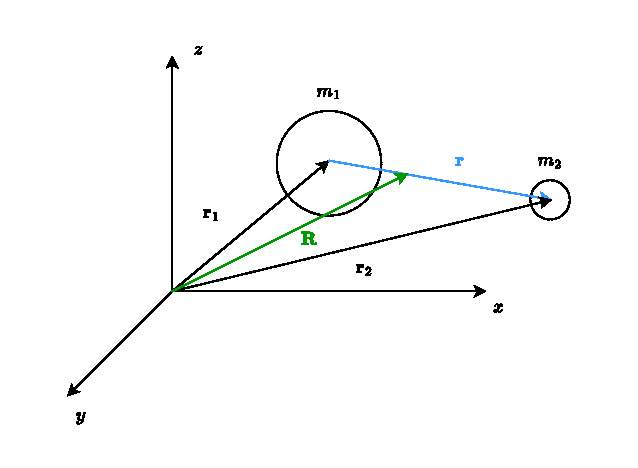
\includegraphics[width=0.8\linewidth]{res/svg/two_body_problem_start.drawio}
  \caption{Two body problem}
\end{figure}
In principle we start from $3n= 6$ degrees of freedom, which means that $\vec{r}_1$ and $\vec{r}_2$ can be used as $q_{\alpha}$, but, in order to use Kőnig's theorem we can define the coordinate of the centre of mass:
\begin{equation}
  \vec{R} = \dfrac{m_1\vec{r}_1 + m_2\vec{r}_2}{m_1 + m_2}
\end{equation}
Since the potential $V(r)$ only depends on the distance between the objects we can define the vector that goes from $m_1$ to $m_2$ as:
\begin{equation}
  \vec{r} = \vec{r}_2 - \vec{r}_1
\end{equation}
From this we can obtain the transformation equations. First we find $\vec{r_1}$:
\begin{equation}
  \begin{split}
    \vec{R} &= \dfrac{m_1\vec{r}_1 + m_2\vec{r}_2}{m_1 + m_2} \\[8pt]
    \vec{R} - \vec{r}_1 &= \dfrac{m_1\vec{r}_1 + m_2\vec{r}_2}{m_1 + m_2} - \vec{r}_1 \\[8pt]
    \vec{R} - \vec{r}_1 &= \dfrac{\cancel{m_1\vec{r}_1} - \cancel{m_1\vec{r}_1} + m_2\vec{r}_2 - m_2\vec{r}_1}{m_1 + m_2} \\[8pt]
    \vec{R} - \vec{r}_1 &= \dfrac{m_2(\overbrace{\vec{r}_2 - \vec{r}_1}^{\vec{r}})}{m_1 + m_2} \\[8pt]
    \vec{r}_1 &= \vec{R} - \dfrac{m_2}{m_1 + m_2}\vec{r}
  \end{split}
\end{equation}
Same goes for $\vec{r}_2$
\begin{equation}
  \begin{split}
    \vec{R} &= \dfrac{m_1\vec{r}_1 + m_2\vec{r}_2}{m_1 + m_2} \\[8pt]
    \vec{R} - \vec{r}_2 &= \dfrac{m_1\vec{r}_1 + m_2\vec{r}_2}{m_1 + m_2} - \vec{r}_2 \\[8pt]
    \vec{R} - \vec{r}_2 &= \dfrac{\cancel{m_2\vec{r}_2} - \cancel{m_2\vec{r}_2} + m_1\vec{r}_1 - m_1\vec{r}_2}{m_1 + m_2} \\[8pt]
    \vec{R} - \vec{r}_2 &= -\dfrac{m_1(\overbrace{\vec{r}_2 - \vec{r}_1}^{\vec{r}})}{m_1 + m_2} \\[8pt]
    \vec{r}_2 &= \vec{R} + \dfrac{m_1}{m_1 + m_2}\vec{r}
  \end{split}
\end{equation}
We can further simplify those equations by introducing the \textbf{reduced mass} $\mu$:
\begin{equation}
  \mu \defineeq \dfrac{m_1 m_2}{m_2 + m_1}
\end{equation}
And so the transformation equations can be written as:
\begin{equation}
  \begin{cases}
    \vec{r}_1 = \vec{R} - \dfrac{\mu}{m_1}\vec{r} \\[8pt]
    \vec{r}_2 = \vec{R} + \dfrac{\mu}{m_2}\vec{r}
  \end{cases}
\end{equation}
The transformation equations do not depend on time, so the Hamiltonian is the energy and it is conserved. The kinetic energy $T$ is a quadratic function of the velocity since the system does not have any external force and so we can finally apply Kőnig's theorem:
\begin{equation}
  T = T_{CM} + T'
\end{equation}
$T'$ is the kinetic energy in the reference frame of the centre of mass. If we use the transformation equations we can recover those terms:
\begin{equation}
  \begin{split}
    T &= \dfrac{1}{2}m_1\dvec{r}_1^2 + \dfrac{1}{2}m_1\dvec{r}_1^2 = \\[8pt]
    &= \dfrac{1}{2}m_1\brackets{\dvec{R} - \dfrac{\mu}{m_1}\dvec{r}}^2 + \dfrac{1}{2}m_2\brackets{\dvec{R} + \dfrac{\mu}{m_2}\dvec{r}}^2 = \\[8pt]
    &= \dfrac{1}{2}m_1\brackets{\dvec{R}^2 - 2\dfrac{\mu}{m_1}\dvec{r}\dvec{R} + \dfrac{\mu^2}{m_1^2}\dvec{r}^2} + \dfrac{1}{2}m_2\brackets{\dvec{R}^2 + 2\dfrac{\mu}{m_2}\dvec{r}\dvec{R} + \dfrac{\mu^2}{m_2^2}\dvec{r}^2} = \\[8pt]
    &= \dfrac{1}{2}m_1\dvec{R}^2 - \cancel{\mu\dvec{r}\dvec{R}} + \dfrac{\mu^2}{2m_1}\dvec{r}^2 + \dfrac{1}{2}m_2\dvec{R}^2 + \cancel{\mu \dvec{r}\dvec{R}} + \dfrac{\mu^2}{2m_2}\dvec{r}^2 = \\[8pt]
    &= \dfrac{1}{2}\brackets{m_1 + m_2}\dvec{R}^2 + \dfrac{1}{2}\brackets{\mu^2\underbrace{\dfrac{m_1 + m_2}{m_1m_2}}_{\mu}}\dvec{r}^2 = \\[8pt]
    &= \dfrac{1}{2}M\dvec{R}^2 + \dfrac{1}{2}\mu\dvec{r}^2
  \end{split}
\end{equation}
Clearly we have:
\begin{equation}
  \begin{split}
    &T_{CM} = \dfrac{1}{2}M\dvec{R}^2 \\[8pt]
    &T' = \dfrac{1}{2}\mu\dvec{r}^2
  \end{split}
\end{equation}
We can thus construct the Lagrangian of the system for a general potential $V(r)$:
\begin{equation}
  \lagr = T - V = \dfrac{1}{2}M\dvec{R}^2 + \dfrac{1}{2}\mu\dvec{r}^2 - V(r)
\end{equation}
The components of the centre of mass $X, Y, Z$ do not appear in the Lagrangian and so we immediately find that their conjugate momenta $p_X, p_Y, p_Z$ are conserved, thus the total momentum of the centre of mass $\vec{P}$ is conserved, but we know that:
\begin{equation}
  \vec{P} = M\dvec{R}
\end{equation}
And since the mass is constant also $\dvec{R}$ will be a conserved quantity and the centre of mass moves with constant velocity, thus we can ignore this term in the Lagrangian. We define the new Lagrangian as:
\begin{equation}
  \lagr ' = \dfrac{1}{2}\mu\dvec{r}^2 - V(r)
\end{equation}
Since the potential $V(r)$ only depends on the distance of the masses it is spherically simmetric, which implies that the Lagrangian is spherically simmetric and so $L_x, L_y, L_z$ are conserved quantities, but also $\vec{L}$ is conserved. $\vec{L}$ is the angular momentum about the centre of mass:
\begin{equation}
  \vec{L} = \vec{r}\cross \mu\dvec{r}
\end{equation}
And so the orbit must take place in the plane perpendicular to $\vec{L}$.
\begin{figure}[H]
  \centering
  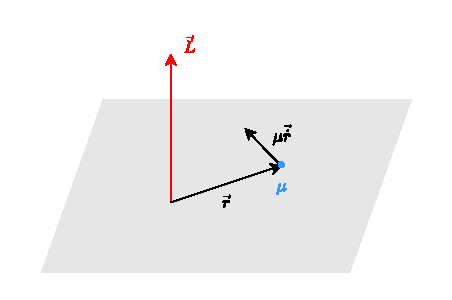
\includegraphics[width=0.6\linewidth]{res/svg/two_body_problem_angular.drawio}
\end{figure}
\begin{figure}[H]
  \centering
  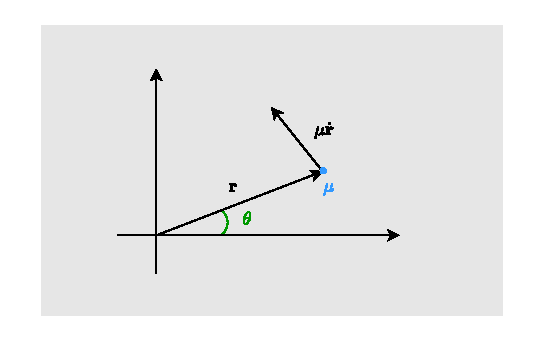
\includegraphics[width=0.6\linewidth]{res/svg/two_body_problem_angular_plane.drawio}
  \caption{Plane orbit}
\end{figure}
Using this fact we can switch to radial coordinates and rewrite the Lagrangian as:
\begin{equation}
  \lagr' = \dfrac{1}{2}\mu\brackets{\dot{r}^2 + r^2\dot{\theta}^2} - V(r)
\end{equation}
Here $\theta$ does not appear and so it is a cyclic coordinate, which means that $p_{\theta}$ is conserved:
\begin{equation}
  p_{\theta} = \pdv{\lagr'}{\dot{\theta}} = \mu r^2 \dot{\theta}
\end{equation}
But this is also the $z$ component of the angular momentum:
\begin{equation}
  \begin{split}
    L_z &= \brackets{\vec{r}\cross \mu\dvec{r}} \cdot \hat{u}_z = \\[8pt]
    &= \sqbr{r\hat{u}_r \cross \mu\brackets{\dot{r}\hat{u}_r + r\dot{\theta}\hat{u}_{\theta}}} \cdot \hat{u}_z = \\[8pt]
    &= \bbrackets{\mu r\dot{r} \cancel{\hat{u}_r \cross \hat{u}_r} + \mu r^2\dot{\theta}\underbrace{\hat{u}_r \cross \hat{u}_{\theta}}_{\hat{u}_z}} \cdot \hat{u}_z = \\[8pt]
    &= \mu r^2\dot{\theta} \hat{u}_z \cdot \hat{u}_z = \mu r^2\dot{\theta}
  \end{split}
\end{equation}
And thus we have:
\begin{equation}
  \dot{\theta} = \dfrac{L_z}{\mu \dot{r}^2}
\end{equation}
Now we can apply \eleref\;to $\lagr'$ for $q_{\alpha} = r$ and see what we get:
\begin{equation}
  \begin{split}
    &\dv{}{t}\pdv{}{\dot{r}}\brackets{\dfrac{1}{2}\mu\brackets{\dot{r}^2 + r^2\dot{\theta}^2} - V(r)} - \pdv{}{r}\brackets{\dfrac{1}{2}\mu\brackets{\dot{r}^2 + r^2\dot{\theta}^2} - V(r)} = \\[8pt]
    &= \mu\dv{\dot{r}}{t} - \mu r\dot{\theta}^2 + \pdv{V}{r}  = \\[8pt]
    &= \mu \ddot{r} - \mu r\dot{\theta}^2 + \pdv{V}{r}
  \end{split}
\end{equation}
Now we can substitute what we got for $\dot{\theta}$:
\begin{equation} \label{ele_twobody}
  \boxed{\mu \ddot{r} - \dfrac{L_z^2}{\mu \dot{r}^3} + \pdv{V}{r} = 0}
\end{equation}
Remember that we want to write this problem as a one dimensional problem, so we need to find a potential of the type:
\begin{equation}
  m\dot{q} = -\pdv{V}{q}
\end{equation}
We can rewrite the term with $L_z$ as:
\begin{equation}
  - \dfrac{L_z^2}{\mu \dot{r}^3} = \pdv{}{r}\brackets{\dfrac{L_z^2}{2\mu \dot{r}^2}}
\end{equation}
From \eqref{ele_twobody} we get:
\begin{equation}
  \mu \ddot{r} = -\pdv{}{r}\brackets{V - \dfrac{L_z^2}{2\mu \dot{r}^2}}
\end{equation}
By multiplying both sides by $\dot{r}$ we get the total time derivative of $\dfrac{1}{2}\mu \dot{r}^2$ on the left side and the total time derivative of the quantity in brackets of the right side since it only depends on $r$. We will that quantity \textbf{effective potential} $V_{\text{eff}}$, since it is not a real potential, but it will serve the purpose of the one dimensional potential that we want to find. We can write:
\begin{equation}
    \begin{split}
        &\mu \ddot{r}\dot{r} = -\pdv{V_{\text{eff}}(r)}{r}\dot{r} \\[8pt]
        &\dv{}{t}\brackets{\dfrac{1}{2}\mu \dot{r}^2} = -\dv{V_{\text{eff}}}{t} \\[8pt]
        &\dv{}{t}\brackets{\dfrac{1}{2}\mu \dot{r}^2 + V_{\text{eff}}} = 0
    \end{split}
\end{equation}
From the last equation we know that the quantity in brackets is conserved. We still have not used the conservation of energy. The total energy is:
\begin{equation}
    E = \dfrac{1}{2}\mu \dot{r}^2 + V - \dfrac{L_z^2}{2\mu \dot{r}^2}
\end{equation}
And so we can find $r$ by integrating. We have:
\begin{equation}
    \begin{split}
        \dfrac{1}{2}\mu \dot{r}^2 = E - V + \dfrac{L_z^2}{2\mu \dot{r}^2} \\[8pt]
        \dot{r}^2 = \dfrac{2}{\mu}\brackets{E - V + \dfrac{L_z^2}{2\mu \dot{r}^2}} \\[8pt]
        \dv{r}{t} = \pm\sqrt{\dfrac{2}{\mu}\brackets{E - V + \dfrac{L_z^2}{2\mu \dot{r}^2}}} \\[8pt]
        \int_{r(0)}^{r(t)}\pm\sqrt{\dfrac{\mu}{2\brackets{E - V + \frac{L_z^2}{2\mu \dot{r}^2}}}}\diff{r} = \int_{0}^{t}\diff{t}
    \end{split}
\end{equation}
If $V(r)$ is known we can solve this integral and get $t$ as a function of $r(t)$:
\begin{equation}
  t = f(r(t)) \xrightarrow{\text{invert}} r = r(t)
\end{equation}
We also need to find $\theta(t)$ to get the transverse velocity:
\begin{equation}
  \begin{split}
    &\dv{\theta}{t} = \dfrac{L_z^2}{\mu \dot{r}^2} \\[8pt]
    &\int_{\theta(0)}^{\theta}\diff{\theta} = \int_{0}^{t}\dfrac{L_z^2}{\mu \dot{r}^2}\diff{t} \\[8pt]
    &\theta(t) = \theta(0) + \int_{0}^{t}\dfrac{L_z^2}{\mu \dot{r}^2}\diff{t}
  \end{split}
\end{equation}
Now we can use the fact that:
\begin{equation}
  \diff{t} = \pm\sqrt{\dfrac{\mu}{2\brackets{E - V + \frac{L_z^2}{2\mu \dot{r}^2}}}}\diff{r}
\end{equation}
We can limit ourselves to the case of $+$ since $L_z$ has a constant sign and so we can ``absorb'' the $\pm$ with the choice of $L_z$. We arrive to the expression:
\begin{equation}
  \theta(t) = \theta(0) + \int_{a}^{b}\dfrac{L_z^2}{\mu \dot{r}^2}\sqrt{\dfrac{\mu}{2\brackets{E - V + \frac{L_z^2}{2\mu \dot{r}^2}}}}\diff{r}
\end{equation}
The limits of the integral change since we made a change of variable. They are unkown for the moment since we have no form of $V$. Now we need the intial conditions:
\begin{itemize}
  \item $r(0) = r_0$
  \item $\dot{r}(0) = \dot{r}_0$
  \item $\theta(0) = \theta_0$
  \item $\dot{\theta}(0) = \dot{\theta}_0$
\end{itemize}
We can fix $\dot{r}_0$ and $\dot{\theta}_0$ with $L_z$ and $E$ since they are conserved:
\begin{equation}
  L_z = \mu r_0^2 \dot{\theta}_0^2 \implies \dot{\theta}_0^2 = \dfrac{L_z}{\mu r_0^2}
\end{equation}
\begin{equation}
  E = \dfrac{1}{2}\mu\dot{r}_0^2 + V_{\text{eff}}(r_0) \implies \dot{r}_0 = \pm\sqrt{\dfrac{2}{\mu}\brackets{E - V_{\text{eff}}(r_0)}}
\end{equation}
In general we have:
\begin{equation}
    \dot{r}(t) = \pm\sqrt{\dfrac{2}{\mu}\brackets{E - V_{\text{eff}}(t)}}
\end{equation}
And so $r(t)$ cannot be a monotonic function, but there must exist a point of inversion. This point is found when the time derivative is zero:
\begin{equation}
    \pm\sqrt{\dfrac{2}{\mu}\brackets{E - V_{\text{eff}}(t)}} = 0 \implies E = V_{\text{eff}}
\end{equation}
This means that when $V_{\text{eff}}$ is equal to the energy we have a point of inversion. Since $V_{\text{eff}} = V + \dfrac{L_z}{2\mu r^2}$ depending on $V$ and $E$ we can have either $1$ or $2$ points of inversion.
\begin{itemize}
    \item If only $1$ point is present we just have a one time motion. The object comes from infinity, orbits the other one for a certain period and then goes away.
    \item If two points of inversion are present the motion of $\mu$ is limited in a certain angular region with a maximum and a minimum
\end{itemize}
Notice that the orbits are not necessarily closed.
\subsection{The Kepler problem}
As an example we will discuss the Kepler problem, which describes how orbits work in the case of a potential of the type:
\begin{equation}
    V(r) = -\dfrac{\alpha}{r}
\end{equation}
This could be for example the gravitational potential or the Coulomb potential. Given this form of $V$ we know that:
\begin{equation}
    V_{\text{eff}} = \dfrac{L_z^2}{2 \mu r^2} - \dfrac{\alpha}{r}
\end{equation}
Qualitatively speaking we know the asymptotic behavior of the effective potential:
\begin{itemize}
    \item At $r \rightarrow 0$ the term with $\dfrac{1}{r^2}$ dominates so $V_{\text{eff}} \rightarrow +\infty$ for $r \rightarrow 0$
    \item For $r \rightarrow +\infty$ the term with $-\dfrac{1}{r}$ dominates so $V_{\text{eff}} \rightarrow -$ for $r \rightarrow 0$ with negative values
    \item There must be a point where $V_{\text{eff}}$ stops decreasing and starts increasing, this is a point of minimum for the effective potential
\end{itemize}
\begin{figure}[H]
  \centering
  \includesvg[width=0.8\linewidth]{res/svg/effectivepotential_sum}
\end{figure}
Let's find the minimum:
\begin{equation}
  \pdv{}{r}\brackets{\dfrac{L_z^2}{2 \mu r^2} - \dfrac{\alpha}{r}} =  \dfrac{\alpha}{r^2} -\dfrac{L_z^2}{\mu r^3}
\end{equation}
Setting this to zero gives:
\begin{equation}
  \dfrac{\alpha}{\cancel{r^2}} =\dfrac{L_z^2}{\mu r^{\cancel{3}}} \implies r = \dfrac{L_z^2}{\mu \alpha}
\end{equation}
If we compare $V_{\text{eff}}$ to a constant value of energy we find that the point of intersection is where $E = V_{\text{eff}}$ and so where $\dot{r} = 0$, which is the inversion point of the orbit. We can distinguish 4 cases.\\
\textbf{Case 1.} In the first case we have $E > 0$.
\begin{figure}[H]
  \centering
  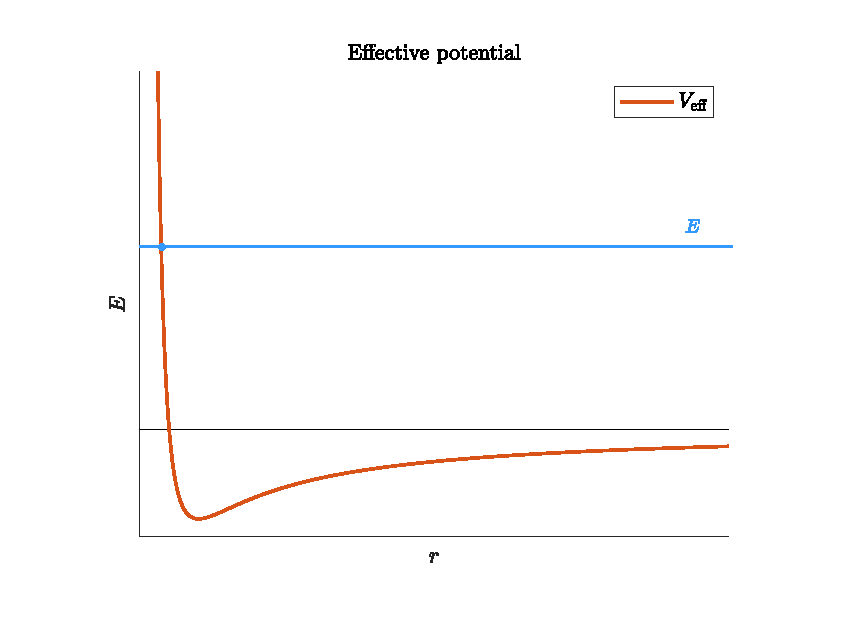
\includegraphics[width=0.6\linewidth]{res/svg/hyperbolic_orbit.drawio}
\end{figure}
There is only one point of inversion and the orbit is hyperbolic.
\begin{figure}[H]
  \centering
  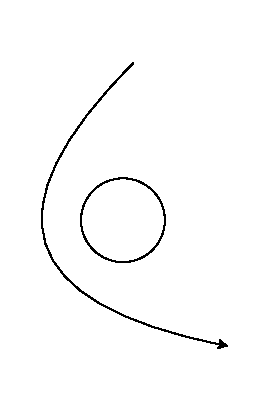
\includegraphics[width=0.2\linewidth]{res/svg/hyperbolic_orbit_drawing.drawio}
\end{figure}
\textbf{Case 2.} In the second case we have $E = 0$.
\begin{figure}[H]
  \centering
  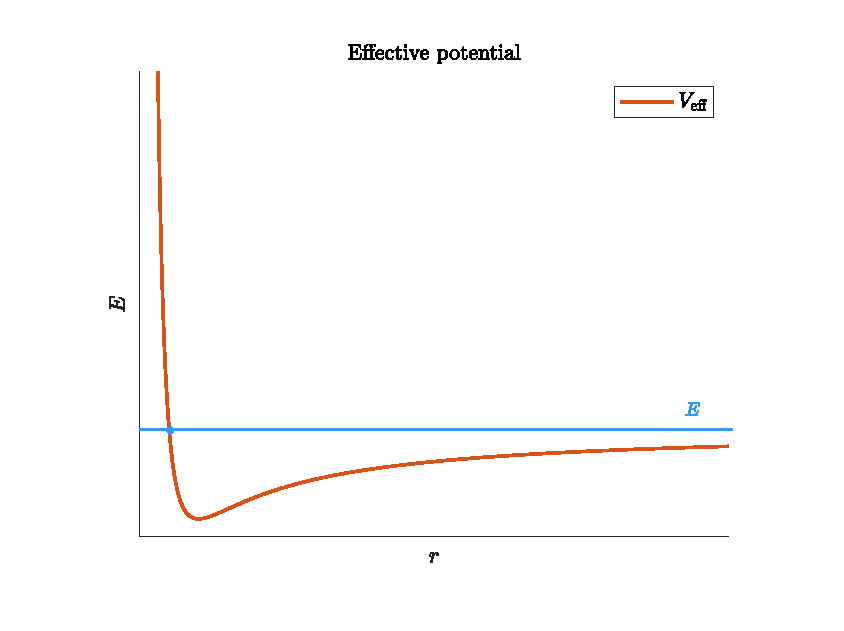
\includegraphics[width=0.6\linewidth]{res/svg/parabolic_orbit.drawio}
\end{figure}
Here we have one point of inversion and we also have that $E=V_{\text{eff}}$ at infinity. This creates a parabolic orbit.
\begin{figure}[H]
  \centering
  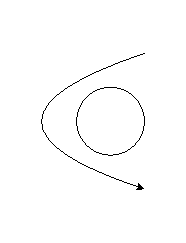
\includegraphics[width=0.2\linewidth]{res/svg/parabolic_orbit_drawing.drawio}
\end{figure}
\textbf{Case 3.} In the third case $E<0$ but it is greater than the minimum of $V_{\text{eff}}$.
\begin{figure}[H]
  \centering
  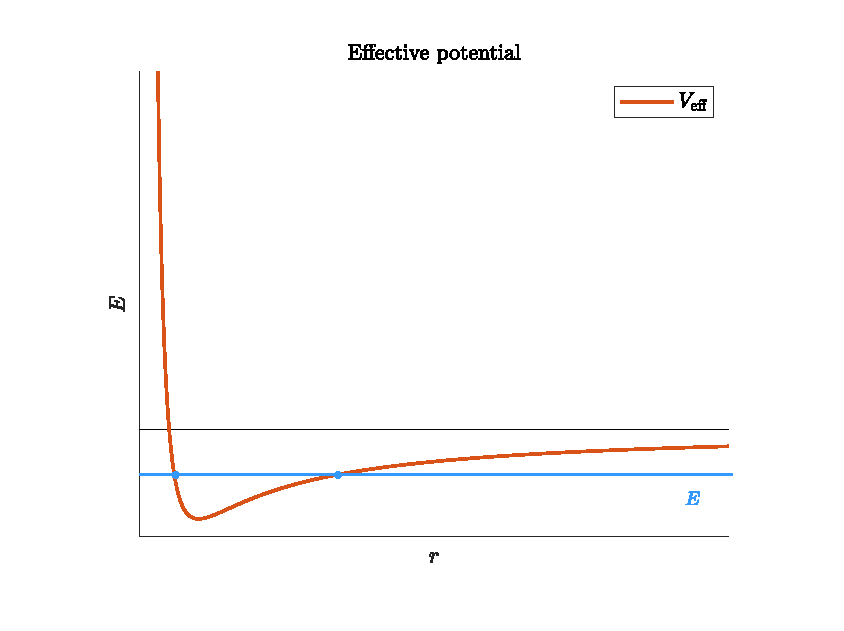
\includegraphics[width=0.6\linewidth]{res/svg/elliptic_orbit.drawio}
\end{figure}
We have two distinct inversion points $r_0$ and $r_1$ which create an elliptical orbit.
\begin{figure}[H]
  \centering
  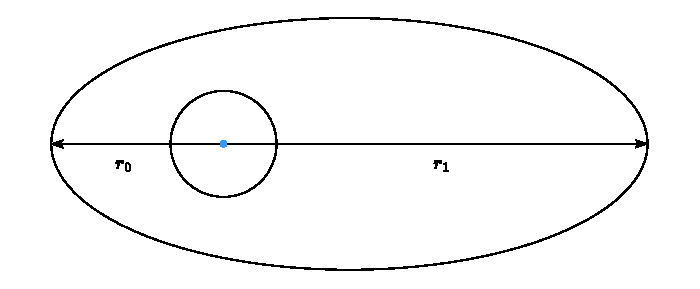
\includegraphics[width=0.6\linewidth]{res/svg/elliptic_orbit._drawing.drawio}
\end{figure}
\textbf{Case 4.} In the fourth case $E<0$ and it is equal to the minimum of $V_{\text{eff}}$.
\begin{figure}[H]
  \centering
  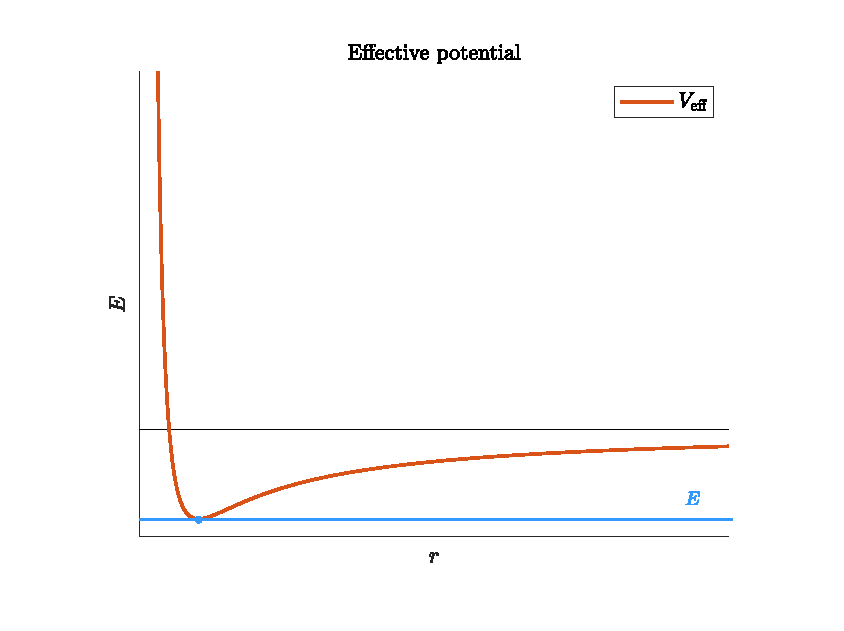
\includegraphics[width=0.6\linewidth]{res/svg/circular_orbit.drawio}
\end{figure}
We have two coincident inversion points which create a circular orbit.
\begin{figure}[H]
  \centering
  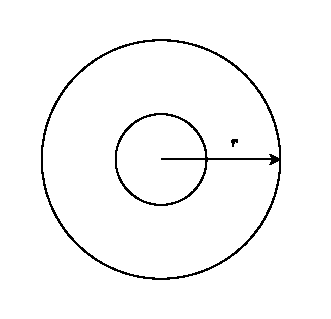
\includegraphics[width=0.4\linewidth]{res/svg/circular_orbit_drawing.drawio}
\end{figure}

\chapter{Canonical transformations}
\section{Point transformations}
Let's now focus on the possible transformations of coordinates.\\
In Lagrangian formalism a generic transformation is:
\begin{equation}
    \{q_{\alpha}\} \longrightarrow \{Q_{\alpha}\}\quad \text{s.t.}\quad Q_{\alpha} = Q_{\alpha}\brackets{q_1,q_2,\dots,q_n,t}
\end{equation}
This is a \textbf{point transformation} in configuration space. We move from $n$ spatial coordinates to $n$ spatial coordinates.\\
In Hamiltonian formalism a generic transformation is:
\begin{equation}
    \begin{Bmatrix}
        q_{\alpha}\\[8pt]
        p_{\alpha}
    \end{Bmatrix} \longrightarrow
    \begin{Bmatrix}
        Q_{\alpha}\\[8pt]
        P_{\alpha}
    \end{Bmatrix}\quad \text{s.t} \quad
    \begin{cases}
        Q_{\alpha} = Q_{\alpha}\brackets{q_1,q_2,\dots,q_n,p_1,p_2,\dots,p_n,t}\\
        P_{\alpha} = P_{\alpha}\brackets{q_1,q_2,\dots,q_n,p_1,p_2,\dots,p_n,t}
    \end{cases}
\end{equation}
This is also a point transformation, but since we are in the phase space the new coordinates can be a mix of both $q_{\alpha}$ and $p_{\alpha}$. Now we can try to figure out if the relations found for $q_{\alpha}$ and $p_{\alpha}$ related to the Poisson brackets are also true for $Q_{\alpha}$ and $P_{\alpha}$.
We want:
\begin{equation}
    \begin{split}
        \pb{q_{\alpha}}{q_{\beta}} &= 0\\
        \pb{p_{\alpha}}{p_{\beta}} &= 0\\
        \pb{q_{\alpha}}{p_{\beta}} &= \delta_{\alpha \beta}
    \end{split} \implies
    \begin{split}
        \pb{Q_{\alpha}}{Q_{\beta}} &= 0\\
        \pb{P_{\alpha}}{P_{\beta}} &= 0\\
        \pb{Q_{\alpha}}{P_{\beta}} &= \delta_{\alpha \beta}
    \end{split}
\end{equation}
For example we want $\pb{Q_{\alpha}}{Q_{\beta}} = 0$. If we explicit the Poisson brackets we have:
\begin{equation}
    \pb{Q_{\alpha}}{Q_{\beta}} = \bigsum_{\gamma} \left(\pdv{Q_{\alpha}}{q_{\gamma}} \pdv{Q_{\beta}}{p_{\gamma}} - \pdv{Q_{\alpha}}{p_{\gamma}} \pdv{Q_{\beta}}{q_{\gamma}} \right)
\end{equation}
This is not always zero, therefor we will look for transformations such that:
\begin{equation}
    \begin{cases}
        \dot{Q}_{\alpha} = \pdv{\tilde{\hamfun}}{P_{\alpha}} \\[8pt]
        \dot{P}_{\alpha} = -\pdv{\tilde{\hamfun}}{Q_{\alpha}}
    \end{cases}
\end{equation}
Transformations that preserve those properties are called \textbf{canonical transformations}. The new Hamiltonian associated to those transformations is sometimes called \textit{k-Hamiltonian}.\\
In which condition this is true?\\
Recall that the \hamiltonref\;come from the \hpquotemath :
\begin{equation}
    \delta \action = \delta \int_{t_1}^{t_2}\lagr \dd{t} = \int_{t_1}^{t_2} \brackets{\bigsum_{\alpha}\dot{q}_{\alpha}p_{\alpha} - \hamfun} \dd{t} =0
\end{equation}
We want the same for the new Hamiltonian:
\begin{equation}
    \delta \tilde{\action} = \delta \int_{t_1}^{t_2}\tilde{\lagr} \dd{t} \int_{t_1}^{t_2} \brackets{\bigsum_{\alpha}\dot{Q}_{\alpha}P_{\alpha} - \tilde{\hamfun}} \dd{t} \overset{!}{=} 0
\end{equation}
\section{Generating functions}
We also know that the new Lagrangian and the old Lagrangian must describe the same system and they have this relation:
\begin{equation}
    \lagr = \tilde{\lagr}+\dv{F}{t}
\end{equation}
So there must exist a function $F$ such that this is true for a transformation to be canonical. These functions are called \textbf{generating functions}.
In principle a generic $F$ can depend on both the old and the new coordinates:
\begin{equation}
    F = F(\vec{q},\vec{p},\vec{Q},\vec{P},t)
\end{equation}
But if all the coordinates were independent we would have $4n$ variables plus time. The maximum number of variables is $2n$ hence there must be at least $2n$ dependent variables.\\
If we know the expression for both the generating function and the transformation equations we are done. This of course is not the interesting case. We can reconstruct the transformation equations just from the expression of $F$. We can distinguish 4 categories of generating functions:
\begin{enumerate}
    \item $F_1 = F_1(\vec{q},\vec{Q},t)$ (\nth{1} type functions)
    \item $F_2 = F_2(\vec{q},\vec{P},t)$ (\nth{2}  type functions)
    \item $F_3 = F_3(\vec{p},\vec{Q},t)$ (\nth{3}  type functions)
    \item $F_4 = F_4(\vec{p},\vec{P},t)$ (\nth{4}  type functions)
\end{enumerate}
From the relation between the Lagrangians we have:
\begin{equation}
    \begin{split}
        \lagr &= \tilde{\lagr}+\dv{F}{t}\\
        \bigsum_{\alpha}p_{\alpha}\dd{q_{\alpha}} - \hamfun\dd{t} &= \bigsum_{\alpha}P_{\alpha}\dd{Q_{\alpha}} - \tilde{\hamfun}\dd{t} + \dd{F}\\
        &\Downarrow \\
        \dd{F} = \bigsum_{\alpha}p_{\alpha}\dd{q_{\alpha}} &- \bigsum_{\alpha}P_{\alpha}\dd{Q_{\alpha}} + \brackets{\tilde{\hamfun}- \hamfun}\dd{t}\\
        &\Downarrow \\
        F &= F(\vec{q},\vec{Q})
    \end{split}
\end{equation}
This means that the generating function in the relation with the Lagrangians is a first type function $F = F_1$. In this case the differential of $F_1$ is:
\begin{equation}
    \dd{F_1} = \bigsum_{\alpha} \pdv{F_1}{q_{\alpha}} \dd{q_{\alpha}} + \bigsum_{\alpha} \pdv{F_1}{Q_{\alpha}} \dd{Q_{\alpha}} + \pdv{F_1}{t} \dd{t}
\end{equation}
And so we get:
\begin{equation} \label{F1_Canonical}
    \begin{cases}
        \pdv{F_1}{q_{\alpha}} = p_{\alpha}\\[8pt]
        \pdv{F_1}{Q_{\alpha}} = -P_{\alpha}\\[8pt]
        \pdv{F_1}{t} = \brackets{\tilde{\hamfun}- \hamfun}
    \end{cases}
\end{equation}
Hence:
\begin{equation}
    \begin{cases}
        p = p(\vec{q},\vec{Q},t)\\
        P = P(\vec{q},\vec{Q},t)
    \end{cases}
\end{equation}
By inverting the first equation we can get:
\begin{equation}
    Q = Q(\vec{q},\vec{p},t)\\
\end{equation}
Substituting this into the second equation we finally get the transformation equations:
\begin{equation}
    \begin{cases}
        Q = Q(\vec{q},\vec{p},t)\\
        P = P(\vec{q},\vec{p},t)
    \end{cases}
\end{equation}
Also from the third equation in \eqref{F1_Canonical} we have:
\begin{equation}
    \tilde{\hamfun} = \hamfun + \pdv{F_1}{t}
\end{equation}
And so if $F_1$ does not depend on time explicitly:
\begin{equation}
    \tilde{\hamfun} = \hamfun
\end{equation}
This means that the Hamiltonians are equal, but we need to keep in mind that $\tilde{\hamfun}$ depends on the new coordinates so if we have a generic $\hamfun$ substituting $Q$ and $P$ instead of $q$ and $p$ \underline{does not} give $\tilde{\hamfun}$. For example:
\begin{equation}
    \hamfun = \dfrac{p^2}{2m} + \dfrac{\alpha}{q} \notimplies \tilde{\hamfun} = \dfrac{P^2}{2m} + \dfrac{\alpha}{Q}
\end{equation}
Instead we need to substitute the expression of the old coordinates in terms of the new one (or viceversa if we have $\tilde{\hamfun}$).\\
Now let $F$ be a generating function of the first type but with:
\begin{equation}
    \begin{cases}
        Q = q\\
        P = P(\vec{q},\vec{p},t)
    \end{cases}
\end{equation}
Then $q$ and $Q$ are not independent, therefor we should have only $n$ independent variables in $F$, but this is not what we want. In order to write $F$ in terms of only independent coordinates we must find a way to express $F$ as a second type function:
\begin{equation}
    F_1(\vec{q},\vec{Q},t) \longrightarrow F_2(\vec{q},\vec{P},t)
\end{equation}
This is just an application of the Legendre transformations:
\begin{equation}
    \begin{split}
        \dd{F_1} &= \bigsum_{\alpha}p_{\alpha}\dd{q_{\alpha}} - \bigsum_{\alpha}P_{\alpha}\dd{Q_{\alpha}} + \brackets{\tilde{\hamfun}- \hamfun}\dd{t}\\
        \dd{\brackets{F_1 + \bigsum_{\alpha}P_{\alpha}Q_{\alpha}}} &= \bigsum_{\alpha}p_{\alpha}\dd{q_{\alpha}}  + \bigsum_{\alpha}Q_{\alpha}\dd{P_{\alpha}} + \brackets{\tilde{\hamfun}- \hamfun}\dd{t}
    \end{split}
\end{equation}
And so:
\begin{equation}
    F_2 = F_1 + \bigsum_{\alpha}P_{\alpha}Q_{\alpha}
\end{equation}
From this, we obtain the relations:
\begin{equation}
    \begin{cases}
        \pdv{F_2}{q_{\alpha}} = p_{\alpha}\\[8pt]
        \pdv{F_2}{P_{\alpha}} = Q_{\alpha}\\[8pt]
        \pdv{F_2}{t} = \pdv{F_1}{t}
    \end{cases}
\end{equation}
As for the first type this means that:
\begin{equation}
    \begin{cases}
        p = p(\vec{q},\vec{P},t)\\
        Q = P(\vec{q},\vec{P},t)
    \end{cases}
\end{equation}
By inverting the first equation we can get:
\begin{equation}
    P = P(\vec{q},\vec{p},t)\\
\end{equation}
Substituting this into the second equation we get the transformation equations:
\begin{equation}
    \begin{cases}
        Q = Q(\vec{q},\vec{p},t)\\
        P = P(\vec{q},\vec{p},t)
    \end{cases}
\end{equation}
Similarly we can find a way to express $F_1$ as a third type function $F_3$. This is again an application of the Legendre transformations:
\begin{equation}
    \begin{split}
        \dd{F_1} = \bigsum_{\alpha}p_{\alpha}\dd{q_{\alpha}} - \bigsum_{\alpha}P_{\alpha}\dd{Q_{\alpha}} + \brackets{\tilde{\hamfun}- \hamfun}\dd{t}\\
    \dd{\brackets{F_1 - \bigsum_{\alpha}q_{\alpha}p_{\alpha}}} = -\bigsum_{\alpha}q_{\alpha}\dd{p_{\alpha}} - \bigsum_{\alpha}P_{\alpha}\dd{Q_{\alpha}} + \brackets{\tilde{\hamfun}- \hamfun}\dd{t}
    \end{split}
\end{equation}
And so:
\begin{equation}
    F_3 = F_1 - \bigsum_{\alpha}q_{\alpha}p_{\alpha}
\end{equation}
From this, we obtain the relations:
\begin{equation}
    \begin{cases}
        \pdv{F_3}{p_{\alpha}} = -q_{\alpha}\\[8pt]
        \pdv{F_3}{Q_{\alpha}} = -P_{\alpha}\\[8pt]
        \pdv{F_3}{t} = \pdv{F_1}{t}
    \end{cases}
\end{equation}
As for the first type, this means that:
\begin{equation}
    \begin{cases}
        q = q(\vec{p},\vec{Q},t)\\
        P = P(\vec{p},\vec{Q},t)
    \end{cases}
\end{equation}
By inverting the first equation, we can get:
\begin{equation}
    Q = Q(\vec{q},\vec{p},t)
\end{equation}
Substituting this into the second equation, we get the transformation equations:
\begin{equation}
    \begin{cases}
        Q = Q(\vec{q},\vec{p},t)\\
        P = P(\vec{q},\vec{p},t)
    \end{cases}
\end{equation}
Finally we can find a way to express $F_1$ as a fourth type function $F_4$. This is a double application of the Legendre transformations (we can think to pass through second type first or third type first and then go to fourth type):
\begin{equation}
    \begin{split}
        \dd{F_1} &= \bigsum_{\alpha}p_{\alpha}\dd{q_{\alpha}} - \bigsum_{\alpha}P_{\alpha}\dd{Q_{\alpha}} + \brackets{\tilde{\hamfun}- \hamfun}\dd{t}\\
        \dd{\brackets{F_1 + \bigsum_{\alpha}P_{\alpha}Q_{\alpha} - \bigsum_{\alpha}q_{\alpha}p_{\alpha}}} &= -\bigsum_{\alpha}q_{\alpha}\dd{p_{\alpha}} + \bigsum_{\alpha}Q_{\alpha}\dd{P_{\alpha}} + \brackets{\tilde{\hamfun}- \hamfun}\dd{t}
    \end{split}
\end{equation}
And so:
\begin{equation}
    F_4 = F_1 + \bigsum_{\alpha}P_{\alpha}Q_{\alpha} - \bigsum_{\alpha}q_{\alpha}p_{\alpha}
\end{equation}
From this, we obtain the relations:
\begin{equation}
    \begin{cases}
        \pdv{F_4}{p_{\alpha}} = -q_{\alpha}\\[8pt]
        \pdv{F_4}{P_{\alpha}} = Q_{\alpha}\\[8pt]
        \pdv{F_4}{t} = \pdv{F_1}{t}
    \end{cases}
\end{equation}
As for the first type, this means that:
\begin{equation}
    \begin{cases}
        q = q(\vec{p},\vec{P},t)\\
        Q = Q(\vec{p},\vec{P},t)
    \end{cases}
\end{equation}
By inverting the first equation, we can get:
\begin{equation}
    P = P(\vec{q},\vec{p},t)
\end{equation}
Substituting this into the second equation, we get the transformation equations:
\begin{equation}
    \begin{cases}
        Q = Q(\vec{q},\vec{p},t)\\
        P = P(\vec{q},\vec{p},t)
    \end{cases}
\end{equation}
\section{Poisson brackets and canonical transformations}
As we anticipated before we want to know how the Poisson brackets act on the new coordinates. In particular, we state this theorem:
\begin{theorem}{}
  A transformation is canonical if and only if the canonical Poisson brackets are invariant
\end{theorem}
This means that they are the same in the old and new coordinates. For example:
\begin{equation}
    \pb{Q_{\alpha}}{P_{\beta}}_{QP} = \delta_{\alpha \beta} \implies \pb{Q_{\alpha}}{P_{\beta}}_{qp} = \delta_{\alpha \beta}
\end{equation}
The subscript represents in respect to what coordinates we are calculating the Poisson brackets. This theorem also as an important corollary:
\begin{corollary}{}
    If the canonical Poisson brackets are invariant then all Poisson brackets are invariant
\end{corollary}
Which means that for any functions $f$ and $g$ in the phase space:
\begin{equation}
    \pb{f}{g}_{QP} = \pb{f}{g}_{qp} = \pb{f}{g}
\end{equation}
In the last notation (which is the usual one) we do not specify the coordinates since it makes no difference.\\
Another relation that is true in general is:
\begin{equation}
    \dv{f}{t} = \pb{f}{\hamfun} + \pdv{f}{t}
\end{equation}
If we are dealing with a function that is also a constant of the motion then:
\begin{equation}
    \pb{f}{\hamfun} = - \pdv{f}{t}
\end{equation}
If this function also does not depend on time explicitly:
\begin{equation}
    \pb{f}{\hamfun} = 0
\end{equation}
\section{Examples}
We will now show some examples of the application of the Legendre transformations and in general of the utility of the generating functions.
\subsection{Ex. 1}
Given a generating function of the first type $F_1 = F_1(\vec{q},\vec{Q},t)$ such that:
\begin{equation}
    F_1 = \bigsum_{\alpha} q_{\alpha}Q_{\alpha}
\end{equation}
By applying \hamiltonref\;and Legendre transformations we get:
\begin{equation}
    \begin{cases}
        Q_{\beta} = \pdv{F_1}{q_{\beta}} = p_{\beta}\\
        q_{\beta} = \pdv{F_1}{Q_{\beta}} = -P_{\beta}
    \end{cases}
\end{equation}
And so the transformation equations are:
\begin{equation}
    \begin{cases}
        Q_{\alpha} = p_{\alpha}\\
        P_{\alpha} = -q_{\alpha}
    \end{cases}
\end{equation}
So this transformation just swaps the momentum and the position coordinates (taking into account some sign changes).
\subsection{Ex. 2}
Given a generating function of the second type $F_2 = F_2(\vec{q},\vec{P},t)$ such that:
\begin{equation}
    F_2 = \bigsum_{\alpha} q_{\alpha}P_{\alpha}
\end{equation}
By applying \hamiltonref\;and Legendre transformations we get:
\begin{equation}
    \begin{cases}
        P_{\beta} = \pdv{F_2}{q_{\beta}} = p_{\beta}\\
        q_{\beta} = \pdv{F_2}{P_{\beta}} = Q_{\beta}
    \end{cases}
\end{equation}
And so the transformation equations are:
\begin{equation}
    \begin{cases}
        Q_{\alpha} = q_{\alpha}\\
        P_{\alpha} = p_{\alpha}
    \end{cases}
\end{equation}
So this transformation is the \textbf{identity transformation} since the new momenta and positions are equal to the old ones.
\begin{equation}
    \underset{\text{Identity}}{\boxed{F_2 = \bigsum_{\alpha} q_{\alpha}P_{\alpha}}}
\end{equation}
\subsection{Ex. 3}
Given a generating function of the second type $F_2 = F_2(\vec{q},\vec{P},t)$ such that:
\begin{equation}
    F_2 = \bigsum_{\alpha} f_{\alpha}(\vec{q},t) P_{\alpha}
\end{equation}
By applying \hamiltonref\;and Legendre transformations we get:
\begin{equation}
    \begin{split}
        p_{\beta} = \pdv{F_2}{q_{\beta}} = \dots\\
        Q_{\beta} = \pdv{F_2}{P_{\beta}} = f_{\beta}(\vec{q},t)
    \end{split}
\end{equation}
So new positions only depend on old positions, hence this is actually a point transformation in configuration space. This is why any point transformation in configuration space is always canonical.
\subsection{Ex. 4}
Now let the Hamiltonian of a system be:
\begin{equation}
    \hamfun = \dfrac{p^2}{2m} + mgq
\end{equation}
\hamiltonref\;give:
\begin{equation}
    \begin{cases}
        \dot{q} = \pdv{\hamfun}{p} = \dfrac{p}{m}\\[8pt]
        \dot{p} = -\pdv{\hamfun}{q} = -mg
    \end{cases}
\end{equation}
Those are just the Newton's equations for a particle in the gravitational potential. Now let's make a transformation:
\begin{equation}
    F_1 = -\dfrac{Q}{q}
\end{equation}
From this we get:
\begin{equation}
    \begin{cases}
        p = \pdv{F_1}{q} = \dfrac{Q}{q^2}\\[8pt]
        P = -\pdv{F_1}{Q} = \dfrac{1}{q}
    \end{cases}
\end{equation}
From this getting the transformation equations is trivial:
\begin{equation}
    \begin{cases}
        Q = pq^2\\[8pt]
        P = \dfrac{1}{q}
    \end{cases}
\end{equation}
We can invert these relations:
\begin{equation}
    \begin{cases}
        q = \dfrac{1}{P}\\
        p = QP^2
    \end{cases}
\end{equation}
And if we substitute back into the old Hamiltonian we get the new expression:
\begin{equation}
    \tilde{\hamfun} = \dfrac{P^4 Q^2}{2m} + \dfrac{mg}{P}
\end{equation}
This again shows that to get the new Hamiltonian we cannot just substitute $Q$ instead of $q$ and $P$ instead of $p$.\\
Also for the new Lagrangian we have:
\begin{equation}
    \begin{split}
        \lagr &= \tilde{\lagr} + \dv{F_1}{t} =\\
        &= \tilde{\lagr} + \dv{}{t}\brackets{-QP} =\\
        &=\tilde{\lagr} - \dot{Q}P - Q\dot{P}
    \end{split}
\end{equation}
Which gives:
\begin{equation}
    \tilde{\lagr} = \lagr + \dot{Q}P + Q\dot{P}
\end{equation}
We want to check that this is a canonical transformation. We can do this by calculating the canonical Poisson brackets in the new and old coordinates. For the new ones:
\begin{equation}
    \begin{split}
        \pb{Q}{P}_{QP} &= \left(\pdv{Q}{Q} \pdv{P}{P} - \cancel{\pdv{Q}{P}} \cancel{\pdv{P}{Q}} \right) = 1\\
        \pb{Q}{Q}_{QP} &= \left(\pdv{Q}{Q} \cancel{\pdv{Q}{P}} - \cancel{\pdv{Q}{P}} \pdv{Q}{Q} \right) = 0\\
        \pb{P}{P}_{QP} &= \left(\cancel{\pdv{P}{Q}} \pdv{P}{P}  -  \pdv{P}{P} \cancel{\pdv{P}{Q}}\right) = 0
    \end{split}
\end{equation}
For the old ones:
\begin{equation}
    \begin{split}
        \pb{Q}{P}_{qp} &= \left(\pdv{Q}{q} \pdv{P}{p} - \pdv{Q}{p} \pdv{P}{q} \right) = \\
        &= \left(\pdv{}{q}(pq^2) \cancel{\pdv{}{p}\left(\dfrac{1}{q}\right)} - \pdv{}{p}(pq^2) \pdv{}{q}\left(\dfrac{1}{q}\right) \right) = \\
        &= \left(- q^2  \left(-\dfrac{1}{q^2}\right) \right) = 1
    \end{split}
\end{equation}
\begin{equation}
    \begin{split}
        \pb{Q}{Q}_{qp} &= \left(\pdv{}{q}(pq^2) \pdv{}{p}(pq^2) - \pdv{}{p}(pq^2) \pdv{}{q}(pq^2) \right) = \\
        &= \left(2pq  q^2 - q^2  2pq \right) = 0
    \end{split}
\end{equation}
\begin{equation}
    \begin{split}
        \pb{P}{P}_{qp} &= \bigsum_{\alpha} \left(\pdv{P}{q_{\alpha}} \pdv{P}{p_{\alpha}} - \pdv{P}{p_{\alpha}} \pdv{P}{q_{\alpha}} \right) = \\
        &= \left(\pdv{}{q}\left(\dfrac{1}{q}\right) \cancel{\pdv{}{p}\left(\dfrac{1}{q}\right)} - \cancel{\pdv{}{p}\left(\dfrac{1}{q}\right)} \pdv{}{q}\left(\dfrac{1}{q}\right) \right) = 0
    \end{split}
\end{equation}
And so we verified that the canonical Poisson brackets are invariant.
\subsection{Ex. 5}
Now given a transformation we want to prove that it is a canonical transformation:
\begin{equation}
    \begin{cases}
        Q = \ln \brackets{\dfrac{p}{q}}\\
        P = \brackets{-\dfrac{q^2}{2}-1}\dfrac{p}{1}
    \end{cases}
\end{equation}
We have two methods:\\
The \textbf{first method} will just be calculating all the Poisson brackets and verifying that they are invariant.\\
The Poisson brackets in the new coordinates will always be trivial:
\begin{equation}
    \begin{split}
        \pb{Q}{P}_{QP} &= 1\\
        \pb{Q}{Q}_{QP} &= 0\\
        \pb{P}{P}_{QP} &= 0
    \end{split}
\end{equation}
Now we can evaluate the Poisson brackets with respect to the old coordinates:
\begin{equation}
    \begin{split}
        \pb{Q}{P}_{qp} &= \left(\pdv{Q}{q} \pdv{P}{p} - \pdv{Q}{p} \pdv{P}{q} \right) = \\
        &= \bbrackets{\pdv{}{q}\left(\ln\brackets{\dfrac{p}{q}}\right) \pdv{}{p}\left(\brackets{-\dfrac{q^2}{2}-1}\dfrac{p}{q}\right) -\\
        &- \pdv{}{p}\left(\ln\brackets{\dfrac{p}{q}}\right) \pdv{}{q}\left(\brackets{-\dfrac{q^2}{2}-1}\dfrac{p}{q}\right) } = \\
        &= \left(-\dfrac{1}{q}  \brackets{-\dfrac{q^2}{2}-1}  \dfrac{1}{q} - \dfrac{1}{p}  \brackets{-q  \dfrac{p}{q} + \brackets{-\dfrac{q^2}{2}-1}  \dfrac{1}{q}} \right) = \\
        &= \left(\cancel{\dfrac{\dfrac{q^2}{2} + 1}{q^2}} + 1 - \cancel{\dfrac{\dfrac{q^2}{2} + 1}{q^2}} \right) = 1
    \end{split}
\end{equation}
The other ones are trivial:
\begin{equation}
    \pb{Q}{Q}_{qp} = \left(\pdv{Q}{q} \pdv{Q}{p} - \pdv{Q}{p} \pdv{Q}{q} \right) = 0
\end{equation}
\begin{equation}
    \pb{P}{P}_{qp} = \left(\pdv{P}{q} \pdv{P}{p} - \pdv{P}{p} \pdv{P}{q} \right) = 0
\end{equation}

\section{Active canonical transformations}
Up to now we used "passive" transformations, which means that the transformation does not affect the state of the system. Instead, now we will make use of \textbf{active transformations} which are transformations that do not change the axes, but they change the state of the system.\\
First we need to introduce a new definition:
\begin{definition}{Infinitesimal canonical transformations}
    Are transformations that differ from the identity transformation for an infinitesimal amount
\end{definition}
This definition is equivalent to:
\begin{equation}
    F_2 = \bigsum_{\alpha} q_{\alpha}P_{\alpha} + \varepsilon G(\vec{q},\vec{P},t)
\end{equation}
And so we have:
\begin{equation}
    \begin{cases}
        p_{\gamma} = \pdv{F_2}{q_{\gamma}} = P_{\gamma} + \varepsilon\pdv{ G}{q_{\gamma}}\\[10pt]
        Q_{\gamma} = \pdv{F_2}{P_{\gamma}} = Q_{\gamma} + \varepsilon\pdv{ G}{P_{\gamma}}
    \end{cases}
\end{equation}
The term depending on the function $G$ are the infinitesimal changes. Let us define:
\begin{equation}
    \begin{split}
        \delta p_{\gamma} &\defineeq -\varepsilon\pdv{ G}{q_{\gamma}}\\[8pt]
        \delta q_{\gamma} &\defineeq \varepsilon\pdv{ G}{P_{\gamma}}
    \end{split}
\end{equation}
We want to substitute the partial derivative of $G$ with respect to $P_{\gamma}$ with the partial derivative of $G$ with respect to $p_{\gamma}$:
\begin{equation}
    \pdv{G}{p_{\gamma}} = \bigsum_{\alpha} \brackets{\pdv{G}{P_{\alpha}}\pdv{P_{\alpha}}{p_{\gamma}} + \pdv{G}{q_{\alpha}}\cancel{\pdv{q_{\alpha}}{p_{\gamma}}}}
\end{equation}
So from the equation of the generating function:
\begin{equation}
    \begin{split}
        \pdv{P_{\alpha}}{p_{\gamma}} &= \pdv{}{p_{\gamma}}\brackets{p_{\alpha} - \varepsilon\pdv{ G}{q_{\alpha}}} = \\
        &= \delta_{\alpha \gamma} - \underbrace{\varepsilon\pdv{ G}{q_{\alpha}}}_{\text{infinitesimal}}
    \end{split}
\end{equation}
The term underlined is infinitesimal and can be disregarded. This leads to:
\begin{equation}
    \pdv{G}{p_{\gamma}} = \bigsum_{\alpha} \pdv{G}{P_{\alpha}}\delta_{\alpha \gamma} = \pdv{G}{P_{\gamma}}
\end{equation}
Now let's define a new vector containing all the coordinates and momentum:
\begin{equation}
    \vec{\eta} \defineeq \begin{pmatrix}
        q_1\\\dots\\q_n\\p_1\\\dots\\p_n
    \end{pmatrix}
    \quad n+n = 2n \quad \text{elements}
\end{equation}
In this way we can write in a compact form:
\begin{equation}
    \delta \vec{\eta} = \varepsilon \pb{\eta}{G}
\end{equation}
Where, by using the Poisson brackets on the vector we mean that we apply them between every component and $G$. Let's for example choose a particular form of $G$:
\begin{equation}
    G = p_i
\end{equation}
Then only the $q_i$ component of the vector $\delta \vec{\eta}$ has value, the rest of the components are zero:
\begin{equation}
    \delta \vec{\eta} = \begin{pmatrix}
        0\\\dots\\\varepsilon\\0\\\dots\\0
    \end{pmatrix}
\end{equation}
What if $q_i$ is a collective coordinate? Let's take for example $x_{CM}$ then $p_i = P_x$ which is the $x$ component of the total linear momentum. $P_x$ generates a translation of the system as a whole along the $x$ axis. In general $\vec{P}$ generates a translation along his direction (in real space). Let's also notice that if $q_i = x_{CM}$ is a collective coordinate and is cyclic then its corresponding momentum $p_i = P_x$ is conserved and also:
\begin{equation}
  \pdv{\hamfun}{x_{CM}}=0
\end{equation}
Therefore $\hamfun$ does not change. Every conserved quantity is the generator of an infinitesimal displacement that does not change the Hamiltonian. Let's make another example.\\
Let us now consider an angular coordinate $q_i$ such that the associated momentum $p_i$ is a rotation of the system as a whole. If $q_i$ is also cyclic then the Hamiltonian is invariant to rotations along the axis of rotation identified by $p_i$. To make a more concrete example we take $q_i = \theta$ such that $\theta$ is cyclic and $p_i = L_z$, then the Hamiltonian is invariant with respect to rotations along the $z$ axis.\\
Now instead let's take another specific form of the function $G$ in particular let's say that $G= \hamfun$, then:
\begin{equation}
  \delta \vec{\eta} = \varepsilon\pb{\eta}{\hamfun} = \varepsilon\dv{\vec{\eta}}{t}
\end{equation}
And also:
\begin{equation}
  \begin{split}
      \delta p_{\alpha} &\defineeq -\varepsilon\pdv{\hamfun}{q_{\alpha}} = \varepsilon \dot{p}_{\alpha}\\[8pt]
      \delta q_{\alpha} &\defineeq \varepsilon\pdv{\hamfun}{P_{\alpha}} = \varepsilon \dot{q}_{\alpha}
  \end{split}
\end{equation}
If we have a function $[F_2] = \unit{\joule  \cdot \second}$ then $F_2$ will be in the form:
\begin{equation}
  F_2 = \bigsum_{\alpha}\brackets{\dots} + \varepsilon \hamfun
\end{equation}
And so the infinitesimal term $\varepsilon$ is an infinitesimal displacement in time. And so we can understand that the Hamiltonian is the generator of the infinitesimal time evolution.\\
Now let's notice one more thing about the Hamiltonian. If we let the Hamiltonian be the generating function we can either have $\hamfun$ to be explicitly depend on time or not. If $\hamfun$ does depend on time explicitly then:
\begin{equation}
  \dv{\hamfun}{t} = \cancel{\pb{\hamfun}{\hamfun}} + \pdv{\hamfun}{t} \quad \implies \quad  \dv{\hamfun}{t} = \pdv{\hamfun}{t}
\end{equation}
And so the transformation generated by the Hamiltonian changes the Hamiltonian itself. Instead, if $\hamfun$ does not depend on time explicitly:
\begin{equation}
  \dv{\hamfun}{t} = 0
\end{equation}
Which means that the Hamiltonian is a constant of the motion and the transformation leave $\hamfun$ unaffected.\\
Let us now consider a generic function $u(q,p,t)$ in the phase space such that $u$ does not depend on time explicitly. Then we can state that:
\begin{equation}
  \dv{u}{t} = \pb{u}{\hamfun} + \cancel{\pdv{u}{t}} \quad \implies \quad  \dv{u}{t} = \pb{u}{\hamfun}
\end{equation}
We now express $u$ as dependent on time, but we know that its "dependence" on time is due to $q$ and $p$ and instead time does not directly appear in the equation fo $u$. And so for an infinitesimal time change we have:
\begin{equation}
  u(t+\dd{t}) - u(t) = \dot{u}\dd{t}
\end{equation}
Since we know what the time derivative of $u$ is we have:
\begin{equation}
  u(t+\dd{t}) - u(t) = \pb{u}{\hamfun}
\end{equation}
So to reconstruct the time evolution of $u$ we just need to know the time evolution of the Hamiltonian. Keep in mind that $u$ is just a generic function, so this argument is valid for any function with the same properties as $u$.
\begin{figure}[H]
  \centering
  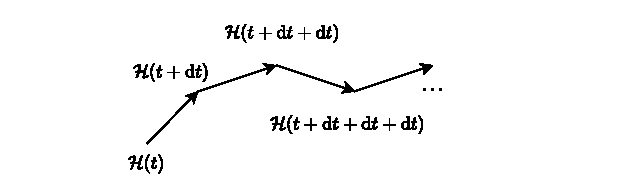
\includegraphics[width=0.6\textwidth]{res/svg/hamiltonian_time_evolution.drawio}
  \caption{Time evolution through Hamiltonian}
\end{figure}
In particular, we can write the Taylor expansion of $u$ and get:
\begin{equation}
  u(t) = u(t_0) + \dv{u}{t}\bigg|_{t_0} (t - t_0) + \frac{1}{2!} \dv[2]{u}{t}\bigg|_{t_0} (t - t_0)^2 + \dots
\end{equation}
We can express the multiple derivatives as:
\begin{equation}
  \begin{split}
    \dv{u}{t} &= \pb{u}{\hamfun}\\
    \dv[2]{u}{t} &= \pb{\pb{u}{\hamfun}}{\hamfun}\\
    \dv[3]{u}{t} &= \pb{\pb{\pb{u}{\hamfun}}{\hamfun}}{\hamfun}\\
    &\dots
  \end{split}
\end{equation}
We then define the operator $\hat{H}$ such that:
\begin{equation}
  \hat{H} = \pb{}{\hamfun}
\end{equation}
And so we can write the Taylor series as:
\begin{equation}
  \begin{split}
    u(t) &= u(t_0) + \hat{H}u(t)\bigg|_{t_0} (t - t_0) + \frac{1}{2!} \hat{H}^2u(t)\bigg|_{t_0} (t - t_0)^2 + \dots =\\
    &= \bigsum_{k=0}^\infty \dfrac{1}{k!} \hat{H}^k u(t)\bigg|_{t_0}(t - t_0)^k =\\
    &= u(t_0)\bigsum_{k=0}^\infty \dfrac{1}{k!} \hat{H}^k (t - t_0)^k \defineeq u(t_0) \efunction^{\brackets{t-t_0}\hat{H}}
  \end{split}
\end{equation}
Keep in mind that the last step is more of a "definition" consistent with the fact that we would get exactly the Taylor series of the exponential if we replaced $\hat{H}$ with a usual variable.
This formula is the classical counterpart of the quantum mechanical "propagator". In particular, we notice that in both cases the formula contains the Hamiltonian (the operator made from the Poisson brackets in the classical case and the operator associated to the Hamiltonian in the quantum case) and also that both are used to get the time evolution of something.

\chapter[H-J Equation]{Hamilton-Jacobi equation}
\section{Derivation of the Hamilton-Jacobi equation}
In this final section regarding analytical mechanics we aim to prove and understand the so-called ``Hamilton-Jacobi equation'', which is the most abstract way of thinking about mechanics. Up to now we defined action as:
\begin{equation}
  \action = \int_{t_1}^{t_2}\lagr\brackets{\vec{q},\dvec{q},t} \dd{t}
\end{equation}
Which means that we think about action as a functional. Now we want to express the same quantity as a function of time and to do so, we need to slightly change our definition:
\begin{equation}
  \action \defineeq \int_{t_0}^{t}\lagr\brackets{\vec{q},\dvec{q},\tau} \dd{\tau}
\end{equation}
We need to remember that the integral of action \underline{must} be calulated along the actual path of the system we are dealing with, but with this definition, in principle, we can obtain $\action$ as a function of time. In particular, we want to prove that $\action$ is a function of both time and all the $q_{\alpha}$.
\begin{proof}
  The proof for the time dependence is trivial since:
  \begin{equation}
    \dv{\action}{t} = \lagr
  \end{equation}
  For the dependence on $q_{\alpha}$ we can imagine changing the coordinates without changing the actual path and the time:
  \begin{figure}[H]
    \centering
    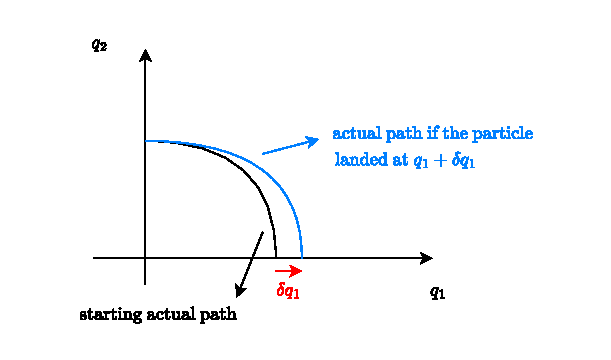
\includegraphics[width=0.6\textwidth]{res/svg/path_change_hamjac.drawio}
    \caption{Path change}
\end{figure}
How does $\action$ change for the two trajectories?
\begin{equation}
  \delta \action = \int_{t_0}^{t}\cancel{\bigsum_{\alpha}\brackets{\pdv{\lagr}{q_{\alpha}}-\dv{}{\tau}\pdv{\lagr}{\dot{q}_{\alpha}}}}\delta q_{\alpha} \dd{\tau} + \int_{t_0}^{t} \dv{}{\tau} \brackets{\bigsum_{\alpha} \pdv{\lagr}{\dot{q}_{\alpha}}\delta q_{\alpha}} \dd{\tau}
\end{equation}
We cancel the first part since when we are integrating over the actual path the \eleref\;are true. We then get:
\begin{equation}
  \begin{split}
    \delta \action &= \int_{t_0}^{t}\dv{}{\tau}\brackets{\bigsum_{\alpha} \pdv{\lagr}{\dot{q}_{\alpha}}\delta q_{\alpha}} \dd{\tau}\\[8pt]
    &= \bigsum_{\alpha} \pdv{\lagr}{\dot{q}_{\alpha}}\delta q_{\alpha}\bigg|_{t_0}^t =\\[8pt]
    &= \bigsum_{\alpha} \pdv{\lagr(t)}{\dot{q}_{\alpha}}\delta q_{\alpha}(t) =\\[8pt]
    &= \bigsum_{\alpha} p_{\alpha} \delta {q_{\alpha}}
  \end{split}
\end{equation}
When we evaluate at $t_0$ the variation is zero since the extremes are fixed. From the final result we have that:
\begin{equation}
  \pdv{\action}{q_{\alpha}} = p_{\alpha}
\end{equation}
And so $\action$ depends on $q_{\alpha}$
\end{proof}
Now we proved that:
\begin{equation}
  \begin{split} \label{e:dvS}
    \dv{\action}{t} &= \bigsum_{\alpha} \pdv{\action}{q_{\alpha}}\dot{q}_{\alpha} + \pdv{\action}{t} =\\[8pt]
    &= \bigsum_{\alpha} p_{\alpha}\dot{q}_{\alpha} + \pdv{\action}{t}
  \end{split}
\end{equation}
But we also know by definition that:
\begin{equation} \label{e:dvS=L}
  \dv{\action}{t} = \lagr
\end{equation}
And so combining \eqref{e:dvS} and \eqref{e:dvS=L} we get:
\begin{equation}
  \lagr = \bigsum_{\alpha} p_{\alpha}\dot{q}_{\alpha} + \pdv{\action}{t} \implies \underbrace{\lagr - \bigsum_{\alpha} p_{\alpha}\dot{q}_{\alpha}}_{-\hamfun} = \pdv{\action}{t}
\end{equation}
And so:
\begin{equation}
  \hamfun (q_{\alpha}, p_{\alpha},t) = -\pdv{\action}{t}
\end{equation}
But we also have that $p_{\alpha}$ is the partial time derivative of $\action$. From this we can get the \textbf{Hamilton-Jacobi equation}:
\begin{equation} \label{e:hamiltonjacobi}
  \boxed{\hamfun \brackets{q_{\alpha}, \pdv{\action}{t},t} = -\pdv{\action}{t}}
\end{equation}
This equation is a single partial differential equation that contains all the information of the system. In principle solving this equation makes us able to find the equations of the motion. Unfortunately this equation can be very difficult to solve.
\subsection{Hamilton-Jacobi and canonical transformations}
Let's now think about when we can easily find the equations of the motion in Hamilton's formalism.
\begin{enumerate}
  \item $\hamfun$ is constant and all the coordinates are cyclic.\\
  In this case:
  \begin{equation}
    \dot{p}_{\alpha} = -\pdv{\hamfun}{q_{\alpha}} = 0 \quad \text{(all the momenta are constant)}
  \end{equation}
  And so we have that $p_{\alpha} = Q_{\alpha}$. In this way deriving with respect to the $p_{\alpha}$ just gives us constant numbers and so:
  \begin{equation}
    \dot{q}_{\alpha} = \pdv{\hamfun}{p_{\alpha}} = b_{\alpha} \quad \text{(linear motion of all the coordinates)}
  \end{equation}
  \item $\hamfun$ may be whatever, but all the $q_{\alpha}$ and $p_{\alpha}$ are constant:
  \begin{equation}
    \begin{split}
      \dot{q}_{\alpha} &= 0\\[8pt]
      \dot{p}_{\alpha} &= 0
    \end{split}
  \end{equation}
\end{enumerate}
Let's make an example for the second case.
\subsubsection{Ex. Free particle in 1-D}
Let's suppose that:
\begin{equation}
  \hamfun = \dfrac{p^2}{2m}
\end{equation}
We get:
\begin{equation}
  \begin{split}
    \dot{q} &= \pdv{\hamfun}{p} = \dfrac{p}{m}\\[8pt]
    \dot{p} &= -\pdv{\hamfun}{q} = 0
  \end{split}
\end{equation}
Since $p$ is constant it must be that $p = p_0$ where $p_0$ is the intial value $p(t=0)$. From this it is easy to find the equation of $q$:
\begin{equation}
  q = q_0 + \dfrac{p_0}{m}t
\end{equation}
Let's now make use of this canonical transformation:
\begin{equation}
  \begin{cases}
    Q &= q - \dfrac{p}{m}t\\[8pt]
    P &= p
  \end{cases}
\end{equation}
Let's check if this transformation is indeed canonical:
\begin{equation}
  \begin{split}
    \pb{Q}{P} &= \brackets{\pdv{Q}{q}\pdv{P}{p} - \pdv{Q}{p}\cancel{\pdv{P}{q}}} = \brackets{\pdv{}{q}\brackets{q - \dfrac{p}{m}t}\pdv{}{p}\brackets{p}}= 1\\
    \pb{Q}{Q} &= \brackets{\pdv{Q}{q}\pdv{Q}{p} - \pdv{Q}{p}\pdv{Q}{q}} = \\
    &= -\dfrac{t}{m} - \brackets{-\dfrac{t}{m}} = 0\\
    \pb{P}{P} &= \brackets{\cancel{\pdv{P}{q}}\pdv{P}{p} - \pdv{P}{p}\cancel{\pdv{P}{q}}} = 0
  \end{split}
\end{equation}
Thus, the transformation satisfies the canonical Poisson bracket relations.\\
We can also try to find a generating function. Since $p = P$ we cannot use a function of the type $F(p,P)$ since the variables wouldn't be independent. Let's choose a first type function:
\begin{equation}
  \begin{split}
    p &= \pdv{F_1}{q}\\[8pt]
    P &= -\pdv{F_1}{Q}
  \end{split}
\end{equation}
We also knwo that the new Lagrangian will be:
\begin{equation}
  \begin{split}
    \lagr &= \tilde{\lagr} + \dv{F_1}{t}\\[8pt]
    p\dot{q} - \hamfun &= P\dot{Q} - \tilde{\hamfun} + \dv{F_1}{t}
  \end{split}
\end{equation}
And so substituting the equations of the transformation:
\begin{equation}
  \begin{split}
    p\dot{q} - \hamfun &= p \dv{}{t}\brackets{Q + \dfrac{p}{m}t} - \dfrac{p^2}{2m} =\\
    &= p\dot{Q} + \dfrac{p\dot{p}}{m}t + \dfrac{p^2}{m} - \dfrac{p^2}{2m} =\\
    &= P\dot{Q} + \dfrac{p\dot{p}}{m}t + \dfrac{p^2}{2m}=\\
    &= P\dot{Q} + \dv{}{t}\bbrackets{\underbrace{\dfrac{p^2}{2m}t}_{F_1}} + \underbrace{0}_{\tilde{\hamfun}}
  \end{split}
\end{equation}
From the transformation equations we have:
\begin{equation}
  F_1 = \dfrac{p^2}{2m}t = \dfrac{m\cancel{^2}(q-Q)^2}{2\cancel{m} t\cancel{^2}}\cancel{t} = \dfrac{m(q-Q)^2}{2t}
\end{equation}
We can verify that this function is actually the action. We know that this must be true:
\begin{equation}
  \begin{split}
    \cancel{\tilde{\hamfun}} - \hamfun &= \pdv{F_1}{t}\\
    \hamfun &= -\pdv{F_1}{t}\\
  \end{split}
\end{equation}
Substituting the functional form we got for $F_1$:
\begin{equation}
  -\pdv{F_1}{t} = -\pdv{}{t}\brackets{\dfrac{m(q-Q)^2}{2t}} = \dfrac{m(q-Q)^2}{2t^2} = \dfrac{p^2}{2m}
\end{equation}
And so this transformation is valid. Now we also notice that we actually wrote the \hamjacref\;equation for $F_1$ and so $F_1$ is indeed the action.
\subsubsection{General statement}
From this example we can try to find a more general approach. In particular, we start from the old coordinates and we want:
\begin{equation}
  \begin{split}
    \begin{Bmatrix}
      q_{\alpha}\\
      p_{\alpha}
    \end{Bmatrix} \longrightarrow
    \begin{Bmatrix}
      Q_{\alpha}\\
      P_{\alpha}
    \end{Bmatrix}\\
    \text{s.t.} \quad \dot{Q}_{\alpha} = 0, \dot{P}_{\alpha} = 0
  \end{split}
\end{equation}
In this way the new coordinates are just numbers:
\begin{equation}
  \begin{split}
    Q_{\alpha} = b_{\alpha}\\
    P_{\alpha} = a_{\alpha}
  \end{split}
\end{equation}
And also the new Hamiltonian must be zero since:
\begin{equation}
  \begin{cases}
    \dot{Q}_{\alpha} = \pdv{\tilde{\hamfun}}{P_{\alpha}} = \pdv{\tilde{\hamfun}}{a_{\alpha}} = 0\\[8pt]
    \dot{P}_{\alpha} = -\pdv{\tilde{\hamfun}}{Q_{\alpha}} = -\pdv{\tilde{\hamfun}}{b_{\alpha}} = 0
  \end{cases}
\end{equation}
Let's try to find the generating function of this transformation by supposing that it is a type 2 function $F_2(\vec{q},\vec{P},t)$.
From the theory of canonical transformations we know that:
\begin{equation} \label{propertiesf2}
  \begin{split}
    \cancel{\tilde{\hamfun}} - \hamfun &= \pdv{F_2}{t}\\[8pt]
    p_{\alpha} &= \pdv{F_2}{q_{\alpha}}\\[8pt]
    Q_{\alpha} &= \pdv{F_2}{P_{\alpha}}
  \end{split}
\end{equation}
From the first equation:
\begin{equation}
  \hamfun \brackets{q_{\alpha}, p_{\alpha},t}= -\pdv{F_2}{t}
\end{equation}
But from the second equation we get:
\begin{equation}
  \hamfun \brackets{q_{\alpha}, \pdv{F_2}{q_{\alpha}},t}= -\pdv{F_2}{t}
\end{equation}
Again this is the \hamjacref\;equation and the function $F_2$ is called \textbf{Hamilton's principal function} and is denoted with $\action$:
\begin{equation}
  \hamfun \brackets{q_{\alpha}, \pdv{\action}{q_{\alpha}},t}= -\pdv{\action}{t}
\end{equation}
As we anticipated this equation has some fundamental properties:
\begin{itemize}
  \item It is 1 first order PDE
  \item It has $n+1$ integration constant, but one is actually trivial since it is just a generic number and we can ignore it. Thus, we have $n$ ``true'' integration constants
  \item $\action$ is of the second type $\action = \action(\vec{q},\vec{P},t)$
\end{itemize}
From these properties we know that $\action$ depends on the $n$ integration constants $k_{\alpha}$ which depend on the various $P_{\alpha}$. We can identify all the integration constants as the values of $P_{\alpha} = a_{\alpha}$ and so $k_{\alpha} = a_{\alpha}$.\\
Now we want to find the equations of $q_{\alpha}$ and $p_{\alpha}$ as functions of the constant numbers $b_{\alpha}$ and $a_{\alpha}$. Going back to \eqref{propertiesf2}:
\begin{equation}
  b_{\alpha} = Q_{\alpha} = \pdv{\action}{P_{\alpha}}
\end{equation}
And so $b_{\alpha} = b_{\alpha}(\vec{q},\vec{a},t)$. Inverting this equation we have $q_{\alpha} = q_{\alpha}(\vec{b},\vec{a},t)$. But we already knew that $p_{\alpha} = p_{\alpha}(\vec{q},\vec{a},t)$ and so substituting the equation found for $q_{\alpha}$ we have:
\begin{equation}
  \begin{split}
    q_{\alpha} = q_{\alpha}(\vec{b},\vec{a},t)\\[8pt]
    p_{\alpha} = p_{\alpha}(\vec{b},\vec{a},t)
  \end{split}
\end{equation}
Which is what we wanted. Now to determine what the constants are we set the intial conditions, which correspond to when $t=0$:
\begin{equation}
  \begin{cases}
    q_{\alpha}(t=0)= q_{\alpha 0} = q_{\alpha}(\vec{b},\vec{a},0)\\[8pt]
    p_{\alpha}(t=0)= p_{\alpha 0} = p_{\alpha}(\vec{b},\vec{a},0)
  \end{cases}
\end{equation}
By inverting those equations we get the integration constants:
\begin{equation}
  \begin{cases}
    a_{\alpha} = a_{\alpha}(\vec{q}_0,\vec{p}_0,0)\\[8pt]
    b_{\alpha} = b_{\alpha}(\vec{q}_0,\vec{p}_0,0)
  \end{cases}
\end{equation}
Since we found that the equations of the motion only depend on the constants $a_{\alpha}$ and $b_{\alpha}$ we have:
\begin{equation}
  \begin{cases}
    q_{\alpha} = q_{\alpha}(\vec{q}_0,\vec{p}_0,t)\\[8pt]
    p_{\alpha} = p_{\alpha}(\vec{q}_0,\vec{p}_0,t)
  \end{cases}
\end{equation}
This is the final solution. In particular this last equation finally makes us understand that the equations of the motion only depend on the initial conditions.
\subsection{Hamilton-Jacobi and the Schrödinger equation}
It is possible to prove that the Schrödinger equation is the quantum counterpart of the classical Hamilton-Jacobi equation. In particular:
\begin{equation}
  \text{Schrödinger equation} \quad \xrightarrow{\text{classical limit}} \quad \text{Hamilton-Jacobi equation}
\end{equation}
For 1 particle:
\begin{equation}
  \begin{split}
    \hamfun &= \dfrac{p^2}{2m} + V\\[8pt]
    \hat{H} &= -\dfrac{\hbar^2}{2m} \lap + V \rightarrow -\dfrac{\hbar^2}{2m} \pdv[2]{}{q} + V
  \end{split}
\end{equation}
Now let:
\begin{equation}
  \Psi(q,t) = \efunction^{(i/ \hbar) \action(q,t)}
\end{equation}
Where $\action = a + ib$ is a complex number. Using Schrödinger equation, for the time derivative part we have:
\begin{equation}
  \begin{split}
    \pdv{\Psi}{t} &= \efunction^{(i/ \hbar) \action} \dfrac{i}{\hbar}\pdv{\action}{t}\\[8pt]
    i\hbar\pdv{\Psi}{t} &= -\pdv{\action}{t} \Psi
  \end{split}
\end{equation}
For the part with the Hamiltonian operator we have:
\begin{equation}
  \begin{split}
    \pdv{\Psi}{t} &= \brackets{\dfrac{i}{\hbar}}\efunction^{(i/ \hbar) \action} \pdv{\action}{q}\\[8pt]
    \pdv[2]{\Psi}{t} &= \brackets{\dfrac{i}{\hbar}}^2\efunction^{(i/ \hbar) \action}\brackets{\pdv{\action}{q}}^2 + \brackets{\dfrac{i}{\hbar}}\efunction^{(i/ \hbar) \action} \pdv[2]{\action}{q}=\\
    &= \brackets{\dfrac{i}{\hbar}}^2\brackets{\pdv{\action}{q}}^2 \Psi + \brackets{\dfrac{i}{\hbar}}\pdv[2]{\action}{q} \Psi
  \end{split}
\end{equation}
And so we have:
\begin{equation}
  \begin{split}
    -\pdv{\action}{t} \cancel{\Psi} &= \dfrac{\hbar^2}{2m}\brackets{\dfrac{i}{\hbar}}^2\brackets{\pdv{\action}{q}}^2 \cancel{\Psi} + \dfrac{\hbar^2}{2m}\brackets{\dfrac{i}{\hbar}}\pdv[2]{\action}{q} \cancel{\Psi} + V\cancel{\Psi}\\[8pt]
    -\pdv{\action}{t} &= \dfrac{-1}{2m}\brackets{\pdv{\action}{q}}^2  + \dfrac{i\hbar}{2m}\pdv[2]{\action}{q} + V
  \end{split}
\end{equation}
If we take the limit for $\hbar \rightarrow 0$ we finally get:
\begin{equation}
  \begin{split}
    -\pdv{\action}{t} &= \dfrac{1}{2m}\brackets{\pdv{\action}{q}}^2  - \cancel{\dfrac{i\hbar}{2m}\pdv[2]{\action}{q}} + V\\[8pt]
    -\pdv{\action}{t} &= \dfrac{1}{2m}\bbrackets{\underbrace{\pdv{\action}{q}}_{p}}^2 + V
  \end{split}
\end{equation}
Which results in the \hamjacref :
\begin{equation}
  \begin{split}
    -\pdv{\action}{t} &= \dfrac{p^2}{2m} + V\\[8pt]
    -\pdv{\action}{t} &= \hamfun \brackets{q_{\alpha}, \pdv{\action}{q_{\alpha}},t}
  \end{split}
\end{equation}
\section{Time independent Hamilton-Jacobi equation}
Now let's ask ourselves. What happens when $\hamfun$ does not depend on time explicitly?\\
We know from previous discussions that if $\hamfun$ does not depend on time explicitly then it is conserved. In this case we also know that the Hamiltonian is a combination of the various $a_{\alpha}$ and $b_{\alpha}$ and so:
\begin{equation}
  \hamfun \brackets{q_{\alpha}, \pdv{\action}{q_{\alpha}}} = K
\end{equation}
From this the \hamjacref\;becomes:
\begin{equation}
  K = -\pdv{\action}{t} \implies \action = -Kt + \hamch
\end{equation}
Now we let $a_1 = P_1 = K$, thus we have:
\begin{equation}
  \action = -a_1t + \hamch(\vec{q},\vec{a})
\end{equation}
The function $\hamch$ is called \textbf{Hamilton's characteristic function}. Since $\hamch$ is the only quantity depending on $q_{\alpha}$:
\begin{equation}
  \pdv{\action}{q_{\alpha}} = \pdv{\hamch}{q_{\alpha}}
\end{equation}
Exploiting this fact we can write the \textbf{time independent Hamilton-Jacobi equation}:
\begin{equation}
  \hamfun \brackets{q_{\alpha},\pdv{\hamch}{q_{\alpha}}} = a_1
\end{equation}
This equation respects some rules and gives us some information:
\begin{itemize}
  \item There are $n$ partial derivatives (no time)
  \item The solution gives $\hamch(\vec{q},\vec{a})$
  \item It's the equation that $\hamch$ must satisfy for this equation to be true:
  \begin{equation}
    \action = -a_1t + \hamch
  \end{equation}
  \item If we solve the equation and find $\hamch$ we can reconstruct $\action$ and since $\action$ is the generating function we can get the equations of motion
\end{itemize}
Let's focus our attention on the last information. We know that $\action$ is a type two generating function that gives us:
\begin{equation}
  \begin{split}
    p_{\alpha} &= \pdv{\action}{q_{\alpha}}\\[8pt]
    Q_{\alpha} &= \pdv{\action}{P_{\alpha}} = \pdv{\action}{a_{\alpha}}
  \end{split}
\end{equation}
For $a_{\alpha} = a_1$:
\begin{equation}
  Q_1 = \pdv{\action}{a_1} = -t + \pdv{\hamch}{a_1}
\end{equation}
For the other $a_{\alpha}$:
\begin{equation}
  Q_{\alpha} = \pdv{\action}{a_{\alpha}} = \pdv{\hamch}{a_{\alpha}}
\end{equation}
Since $Q_{\alpha} = b_{\alpha}$ we can reconstruct $\hamch$ from:
\begin{equation}
  \begin{cases}
    \pdv{\hamch}{a_1} = t + b_1\\[10pt]
    \pdv{\hamch}{a_{\alpha}} = b_{\alpha} \quad \quad (\alpha \neq 1)
  \end{cases}
\end{equation}
By integrating we get:
\begin{equation}
  \begin{cases}
    \hamch = a_1t + a_1b_1 + c_1(a_{\gamma \neq 1}, b_{\gamma \neq 1})\\[8pt]
    \hamch = a_{\alpha}b_{\alpha} + c_{\alpha}(a_{\gamma \neq \alpha}, b_{\gamma \neq \alpha}) \quad \quad (\alpha \neq 1)
  \end{cases}
\end{equation}
In this way we get the expression for $\hamch = \hamch (\vec{b},\vec{a},t)$, but we also know that $\hamch = \hamch (\vec{q},\vec{a})$ and so, in general, any $q_{\alpha}$ must depend on the values of $a_{\alpha}$, $b_{\alpha}$ and time:
\begin{equation}
  q_{\alpha} = q_{\alpha}(\vec{b},\vec{a},t)
\end{equation}
We can apply the same approach for $p_{\alpha}$ and get that:
\begin{equation}
  p_{\alpha} = p_{\alpha}(\vec{b},\vec{a},t)
\end{equation}
By fixing the initial conditions we know that:
\begin{equation}
  \begin{split}
    a &= a(\vec{q}_0,\vec{p}_0)\\[8pt]
    b &= b(\vec{q}_0,\vec{p}_0)
  \end{split}
\end{equation}
Finally, by substituting in the expressions for $q_{\alpha}$ and $p_{\alpha}$ we have that they only depend on the initial conditions:
\begin{equation}
  \begin{cases}
    q_{\alpha} = q_{\alpha}(\vec{q}_0,\vec{p}_0)\\[8pt]
    p_{\alpha} = p_{\alpha}(\vec{q}_0,\vec{p}_0)
  \end{cases}
\end{equation}
Now we aim to show that if $\hamfun$ is a constant of the motion the function $\hamch$ generates a transformation in which every new coordinate $Q_{\alpha}$ is cyclic and so:
\begin{equation}
  \begin{split}
    \dot{P}_{\alpha} = -\pdv{\tilde{\hamfun}}{Q_{\alpha}} = 0\\[8pt]
    \tilde{\hamfun} - \hamfun = \pdv{\hamch}{t} = 0 \implies \hamfun = \tilde{\hamfun} \quad \quad (\hamfun \text{ is unchanged})
  \end{split}
\end{equation}
Let's suppose that a generic type two function leads to this transformation:
\begin{equation}
  \begin{Bmatrix}
    q_{\alpha}\\
    p_{\alpha}
  \end{Bmatrix} \longrightarrow
  \begin{Bmatrix}
    Q_{\alpha} \; \text{is cyclic}\\
    P_{\alpha} = a_{\alpha}
  \end{Bmatrix}
\end{equation}
From the theory of canonical transformations we have that:
\begin{equation}
  \begin{split}
    p_{\alpha} &= \pdv{F_2}{q_{\alpha}}\\[8pt]
    Q_{\alpha} &= \pdv{F_2}{P_{\alpha}} = \pdv{F_2}{a_{\alpha}}
  \end{split}
\end{equation}
Since $\hamfun$ is unchanged we can identify $\hamfun \brackets{q_{\alpha},p_{\alpha}}= a_1$ and so, by substituting we have:
\begin{equation}
  \hamfun \brackets{q_{\alpha},\pdv{F_2}{q_{\alpha}}}= a_1
\end{equation}
Which is the equation that $\hamch$ must satisfy. This means that $F_2$ is $\hamch$ apart from a constant value which we can arbitrarily choose.\\
Let's double-check that $\hamch$ really leads to the desired transformation. From \hamiltonref\;we have:
\begin{equation}
  \begin{split}
    \dot{P}_{\alpha} &= -\pdv{\tilde{\hamfun}}{Q_{\alpha}}\\[8pt]
    \dot{Q}_{\alpha} &= \pdv{\tilde{\hamfun}}{P_{\alpha}}
  \end{split}
\end{equation}
Since $\hamfun = \tilde{\hamfun} = P_1$ the only $\dot{Q}_{\alpha}$ different from zero is the first one:
\begin{equation}
  \dot{Q}_{\alpha} = \pdv{P_1}{P_{\alpha}} = \delta_{1\alpha}
\end{equation}
The first $Q_{\alpha}$ will be:
\begin{equation}
  Q_1 = t + b_1
\end{equation}
The other $Q_{\alpha}$ are constant $Q_{\alpha \neq 1} = b_{\alpha \neq 1}$. We can also notice that $Q_1$ depends on time, actually $Q_1$ \underline{is} time ($\pm$ a shift). Now, once we know the functional form of $\hamch$ we can reconstruct the equations of the motion as usual.\\
We start from the relations given by the generating function:
\begin{equation}
  \begin{split}
    \pdv{\hamch}{q_{\alpha}} &= p_{\alpha} = p_{\alpha}(\vec{q},\vec{a})\\[8pt]
    \pdv{\hamch}{P_{\alpha}} &= Q_{\alpha} = Q_{\alpha}(\vec{q},\vec{a})
  \end{split}
\end{equation}
From the second relation we invert the equations and get:
\begin{equation}
  \begin{split}
    q_{\alpha} &= q_{\alpha}\brackets{Q_{1},Q_{\alpha \neq 1},a_{\alpha}} =\\[8pt]
    &= q_{\alpha}\brackets{b_1 + t,b_{\alpha \neq 1},a_{\alpha}} =\\[8pt]
    &= q_{\alpha}\brackets{b_{\alpha},a_{\alpha},t}
  \end{split}
\end{equation}
By substituting in the first equation we finally get:
\begin{equation}
  \begin{cases}
    q_{\alpha} = q_{\alpha}\brackets{\vec{b},\vec{a},t}\\[8pt]
    p_{\alpha} = p_{\alpha}\brackets{\vec{b},\vec{a},t}
  \end{cases}
\end{equation}
\section{Examples}
\subsection{Harmonic oscillator}
Let's make an example using a very common system, which is composed of a mass attached to a spring moving in a frictionless plane as shown:
\begin{figure}[H]
  \centering
  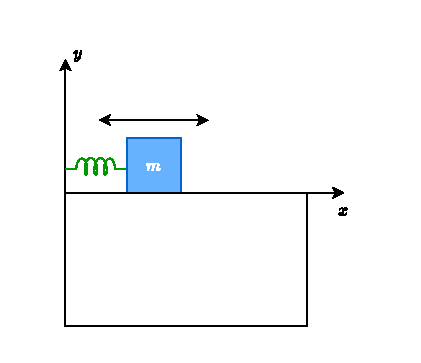
\includegraphics[width=0.7\linewidth]{res/svg/harmonic_oscillator.drawio}
  \caption{Harmonic oscillator}
\end{figure}
The Hamiltonian for this system is:
\begin{equation}
  \hamfun = \dfrac{1}{2}m\dot{q}^2 + \dfrac{1}{2}kq^2
\end{equation}
Which can be written as:
\begin{equation}
  \hamfun = \dfrac{p^2}{2m} + \dfrac{1}{2}m\omega^2q^2
\end{equation}
Now we apply a canonical transformation such that $Q$ and $P$ are constant. We then know that the new Hamiltonian must be zero $\tilde{\hamfun} = 0$. We also know that the Hamiltonian does not depend on time explicitly so we can exploit the time invariant Hamilton-Jacobi equation. This transformation is thus generated by $\action$:
\begin{equation}
  \hamfun \brackets{q_{\alpha},\pdv{\action}{q_{\alpha}}} = -\pdv{\action}{t} = a_1
\end{equation}
We also know that the Hamiltonian is conserved and is the energy, so we can identify $a_1 = E$ and the equation for $\action$ becomes:
\begin{equation}
  \action = -Et + \hamch (q,a) = -Et + \hamch (q,E)
\end{equation}
To find $\hamch$ we substitute in the original Hamiltonian $p = \pdv{\hamch}{q}$:
\begin{equation}
  \hamfun = \dfrac{1}{2m}\brackets{\pdv{\hamch}{q}}^2 + \dfrac{1}{2}m\omega^2q^2 = E
\end{equation}
From which follows:
\begin{equation}
  \begin{split}
    \pdv{\hamch}{q} &= \pm \sqrt{2m\brackets{E - \dfrac{1}{2}m\omega^2q^2}}\\
    \hamch &= \pm \int  \sqrt{2m\brackets{E - \dfrac{1}{2}m\omega^2q^2}} \dd{q}
  \end{split}
\end{equation}
The generating function is:
\begin{equation}
  \action = -Et \pm \int  \sqrt{2m\brackets{E - \dfrac{1}{2}m\omega^2q^2}} \dd{q}
\end{equation}
And so we have that:
\begin{equation}
  p = \pdv{\action}{q} = \pdv{\hamch}{q} = \pm \sqrt{2m\brackets{E - \dfrac{1}{2}m\omega^2q^2}}
\end{equation}
And for the partial derivative with respect to $P$ we can use the fact that $P=E$:
\begin{equation}
  \begin{split}
    \pdv{\action}{P} &= \pdv{\hamch}{E} = -t \pm \int \pdv{}{E} \sqrt{2m\brackets{E - \dfrac{1}{2}m\omega^2q^2}} \dd{q}\\[8pt]
      &= -t \pm \int \dfrac{m}{\sqrt{2m\brackets{E - \dfrac{1}{2}m\omega^2q^2}}} \dd{q}
  \end{split}
\end{equation}
Since this must be equal to a constant:
\begin{equation}
  b = -t \pm \int \dfrac{m}{\sqrt{2m\brackets{E - \dfrac{1}{2}m\omega^2q^2}}} \dd{q}
\end{equation}
Solving the integral gives:
\begin{equation}
  b = -t \pm \dfrac{1}{\omega} \arcsin \brackets{\sqrt{\dfrac{m\omega^2}{2E}}q}
\end{equation}
And so the functional form of $q$ is:
\begin{equation}
  q = \sqrt{\dfrac{2E}{m\omega^2}} \sin \left[\omega\brackets{ t + b}\right]
\end{equation}
By substituting this into $p$ we get:
\begin{equation}
  \begin{split}
    p &= \pm \sqrt{2m\brackets{E - \dfrac{1}{2}m\omega^2 \brackets{\dfrac{2E}{m\omega^2} \sin^2 \left[\omega\brackets{ t + b}\right]}}}=\\[8pt]
    &= \pm \sqrt{2mE\brackets{1 -  \sin^2 \left[\omega\brackets{ t + b}\right]}}=\\[8pt]
    &= \pm \sqrt{2mE\brackets{1 -  \sin^2 \left[\omega\brackets{ t + b}\right]}}
  \end{split}
\end{equation}
Using the trigonometric identity $\sin^2 x + \cos^2 x = 1 $, we have:
\begin{equation}
  \begin{split}
    p &= \pm \sqrt{2m E \cos^2 \left[\omega\brackets{ t + b}\right]}=\\[8pt]
    &= \pm \sqrt{2mE} \cos \left[\omega\brackets{ t + b}\right]
  \end{split}
\end{equation}
Thus, the equations of the motion are:
\begin{equation}
  \begin{cases}
    q = \pm \sqrt{\dfrac{2E}{m\omega^2}} \sin \left[\omega\brackets{ t + b}\right]\\[10pt]
    p = \pm \sqrt{2mE} \cos \left[\omega\brackets{ t + b}\right]
  \end{cases}
\end{equation}
To find the initial conditions we simply put $t=0$ and get:
\begin{equation}
  \begin{split}
    q_0 &= \sqrt{\dfrac{2E}{m\omega^2}} \sin \brackets{\omega b}\\[8pt]
    p_0 &= \pm \sqrt{2mE} \cos \brackets{\omega b}
  \end{split}
\end{equation}
By squaring those equations we get:
\begin{equation}
  \begin{split}
    q_0^2 &= \dfrac{2E}{m\omega^2} \sin^2 \brackets{\omega b} \longrightarrow q_0^2m^2\omega^2 = 2mE \sin^2 \brackets{\omega b}\\[8pt]
    p_0^2 &= 2mE \cos^2 \brackets{\omega b}
  \end{split}
\end{equation}
By adding the two equations:
\begin{equation}
  \begin{split}
    &m^2\omega^2q_0^2 + p_0^2 = 2mE\\[8pt]
    &E = \dfrac{p_0^2}{2m} + \dfrac{1}{2}m\omega^2q_0^2
  \end{split}
\end{equation}
Instead by finding $2mE$ in both equations:
\begin{equation}
  \begin{split}
    &\tan^2 \brackets{\omega b} = \dfrac{m^2\omega^2q_0^2}{p_0^2}\\
    &b = \dfrac{1}{\omega} \arctan \brackets{\dfrac{m\omega q_0}{p_0}}
  \end{split}
\end{equation}
And so the equations of the motion only in terms of the intial conditions can be found by substituting the newly discovered values for $E$ and $b$.\\
If we substitute the functional form of $q$ inside the action we get:
\begin{equation}
  \begin{split}
    \action &= -Et \pm \int \sqrt{2m\brackets{E - \dfrac{1}{2}m\omega^2q^2}} \dd{q}\\[8pt]
    &= -Et \pm \int \sqrt{2m\brackets{E - \dfrac{1}{2}m\omega^2\brackets{\dfrac{2E}{m\omega^2} \sin^2 \left[\omega\brackets{ t + b}\right]}}} \dd{q}\\[8pt]
    &= -Et \pm \int \sqrt{2m\brackets{E - E \sin^2 \left[\omega\brackets{ t + b}\right]}} \dd{q}\\[8pt]
    &= -Et \pm \int \sqrt{2mE \cos^2 \left[\omega\brackets{ t + b}\right]} \dd{q}\\[8pt]
    &= -Et \pm \int \sqrt{2mE} \cos \left[\omega\brackets{ t + b}\right] \dd{q}
  \end{split}
\end{equation}
Now, since $q = \sqrt{\dfrac{2E}{m\omega^2}} \sin \left[\omega\brackets{ t + b}\right]$, we can express $\dd{q}$ as:
\begin{equation}
  \dd{q} = \sqrt{\dfrac{2E}{m\omega^2}} \omega \cos \left[\omega\brackets{ t + b}\right] \dd{t}
\end{equation}
Substituting this into the integral:
\begin{equation}
  \begin{split}
    \action &= -Et \pm \int_0^t \sqrt{2mE} \cos \left[\omega\brackets{ t + b}\right] \sqrt{\dfrac{2E}{m\omega^2}} \omega \cos \left[\omega\brackets{ t + b}\right] \dd{t}\\[8pt]
    &= -Et \pm \int_0^t 2E \cos^2 \left[\omega\brackets{ t + b}\right] \dd{t}\\[8pt]
    &= \int_0^t 2E\brackets{\cos^2 \left[\omega\brackets{ t + b}\right]-\dfrac{1}{2}} \dd{t}
  \end{split}
\end{equation}
Thus, the action becomes:
\begin{equation}
  \action = \int_0^t \underbrace{2E\brackets{\cos^2 \left[\omega\brackets{ t + b}\right]-\dfrac{1}{2}}}_{\lagr} \dd{t}
\end{equation}
And the integrand is the Lagrangian of the system.\\
We could have gotten to this solution by using the Hamilton's characteristic function. From the Hamiltonian relation we know:
\begin{equation}
  E = \dfrac{1}{2m} \brackets{\pdv{\hamch}{q}}^2 + \dfrac{1}{2}m\omega^2q^2 \rightarrow \pdv{\hamch}{q} = \pm \sqrt{2m\brackets{E - \dfrac{1}{2}m\omega^2q^2}}
\end{equation}
And so:
\begin{equation}
  \hamch = \pm \int  \sqrt{2m\brackets{E - \dfrac{1}{2}m\omega^2q^2}} \dd{q}
\end{equation}
Similarly to what we have done before we know that:
\begin{equation}
  Q = \pdv{\hamch}{P} = \pdv{\hamch}{E} = \pm \dfrac{1}{\omega} \arcsin \brackets{\sqrt{\dfrac{m\omega^2}{2E}}q}
\end{equation}
In the new variables this is also true:
\begin{equation}
  \dot{Q} = \pdv{\tilde{\hamfun}}{P} = \pdv{E}{E} = 1 \implies Q = t + b
\end{equation}
From this we have:
\begin{equation}
  t + b = \pm \dfrac{1}{\omega} \arcsin \brackets{\sqrt{\dfrac{m\omega^2}{2E}}q}
\end{equation}
Thus, we get the same results as before for $p$ and $q$:
\begin{equation}
  \begin{cases}
    q = \pm \sqrt{\dfrac{2E}{m\omega^2}} \sin \left[\omega\brackets{ t + b}\right]\\[10pt]
    p = \pm \sqrt{2mE} \cos \left[\omega\brackets{ t + b}\right]
  \end{cases}
\end{equation}

\part{Electromagnetism}
\chapter{Fundamentals}
\section{Maxwell's equations}
As we studied in previous courses all the classical Electromagnetism is contained in some fundamental equations. Those are the Maxwell's equations and the Lorentz force. Maxwell's equations can be either in integral form or differential form. Let's start from the integral form in a vacuum:
\begin{equation} \label{e:int_Maxwell_eq}
  \begin{split}
    &\oint_{\Sigma} \vec{E} \cdot \dd{\vec{\Sigma}} = \dfrac{Q_{enc}}{\epsz}\\[8pt]
    &\oint_{\Sigma} \vec{B} \cdot \dd{\vec{\Sigma}} = 0\\[8pt]
    &\oint_{\gamma} \vec{E} \cdot \dd{\vec{s}} = \dv{}{t}\int_{\Sigma} \vec{B} \cdot \dd{\vec{\Sigma}}\\[8pt]
    &\oint_{\gamma} \vec{B} \cdot \dd{\vec{s}} = \muz i_{enc} + \muz \epsz \dv{}{t}\int_{\Sigma} \vec{E} \cdot \dd{\vec{\Sigma}}
  \end{split}
\end{equation}
The differential (or local) form can be written using various calculus theorem such as stokes theorem or the divergence theorem:
\begin{equation} \label{e:diff_Maxwell_eq}
  \begin{split}
    &\div{\vec{E}} = \dfrac{\rho}{\epsz}\\[8pt]
    &\div{\vec{B}} = 0\\[8pt]
    &\curl{\vec{E}} = -\pdv{\vec{B}}{t}\\[8pt]
    &\curl{\vec{B}} = \muz \vec{J} + \muz \epsz \pdv{\vec{E}}{t}
  \end{split}
\end{equation}
If we want to write Maxwell's equation in materials we must slightly change our definitions. First we must identify new fields which we will call $\vec{D}$ field and $\vec{H}$ field.
Also, inside matter, we can distinguish two ``types'' of charges: the \textbf{free charges} and the \textbf{polarization charges}. This means that for the electric field:
\begin{equation}
  \begin{split}
    Q &\rightarrow Q_f + Q_{pol}\\[8pt]
    \rho &\rightarrow \rho_f + \rho_{pol}
  \end{split}
\end{equation}
For the magnetic field we must distinguish two currents: the \textbf{free current} and the \textbf{magnetic current} (given by the bounded charges and the polarization charges). From this we get that:
\begin{equation}
  \begin{split}
    i &\rightarrow i_f + i_b + i_p\\[8pt]
    \vec{J} &\rightarrow \vec{J}_f + \vec{J}_b + \vec{J}_p
  \end{split}
\end{equation}
Finally we can write Maxwell's equations in matter:
\begin{equation} \label{e:Maxwell_matter}
  \begin{split}
    &\div{\vec{D}} = \rho_f\\[8pt]
    &\div{\vec{B}} = 0\\[8pt]
    &\curl{\vec{E}} = -\pdv{\vec{B}}{t}\\[8pt]
    &\curl{\vec{H}} = \vec{J}_f + \pdv{\vec{D}}{t}
  \end{split}
\end{equation}
Those equations + the Lorentz force can describe all classical Electromagnetism. The expression of the Lorentz force is:
\begin{equation}
  \vec{F} = q (\vec{E} + \vec{v} \cross \vec{B})
\end{equation}
In the stationary case \maxwellref\;become:
\begin{equation} \label{e:stationary_Maxwell_eq}
  \begin{split}
    &\div{\vec{E}} = \dfrac{\rho}{\epsz}\\[8pt]
    &\div{\vec{B}} = 0\\[8pt]
    &\curl{\vec{E}} = 0\\[8pt]
    &\curl{\vec{B}} = \muz \vec{J}
  \end{split}
\end{equation}
The third equation tells us that $\vec{E}$ is an irrotational field in the stationary case. Also, contrary to the general equations, in the stationary case the electric field and the magnetic field are independent.\\
Since the electrostatic field is irrotational we can write it as the gradient of some scalar field since it is always true that:
\begin{equation}
  \curl{(\grad{f})} = 0 \quad \forall f(\vec{r})
\end{equation}
Thus we define the \textbf{electrostatic potential} $\potE$ such that:
\begin{equation}
  \vec{E} = -\grad{\potE}
\end{equation}
Let's now calculate the work of the electromagnetic field in the stationary case over a moving particle with charge $q$. Using the Lorentz force we get:
\begin{equation}
  W_{AB} = \int_{A}^{B} q (\vec{E} + \vec{v} \cross \vec{B}) \cdot \dd{\vec{s}} = \int_{A}^{B} q \vec{E} \cdot \dd{\vec{s}} + \int_{A}^{B} \vec{v} \cross \vec{B} \cdot \dd{\vec{s}}
\end{equation}
Since $\vec{v} \cross \vec{B} \parallel \vec{s}$ the second integral is zero, thus we get:
\begin{equation}
  \begin{split}
    W_{12} &= \int_{A}^{B} q \vec{E} \cdot \dd{\vec{s}} =\\[8pt]
    &= -q \int_{A}^{B} \grad{\potE} \cdot \dd{\vec{s}} =\\[8pt]
    &= -q \int_{A}^{B} \dd{\potE} = q\potE(A) - q\potE(B)
  \end{split}
\end{equation}
So the work of the electrostatic field is just given by the difference between the values of the potential of the two points. Keep in mind that only the difference $\potE(A) - \potE(B)$ has physical meaning. The potential itself can be changed of a constant and the work would be the same. Usually we want to set the reference point for the potential at infinity and so the work necessary to bring a charge from point $A$ to infinity is:
\begin{equation}
  W_{A\rightarrow +\infty} = q\potE(A) - \underbrace{q\potE(+\infty)}_{=\;0} = q\potE(A)
\end{equation}
Now let's imagine a charge fixed at a point $\vec{r}'$ that generates an electrostatic field in space.
\begin{figure}[H]
  \centering
  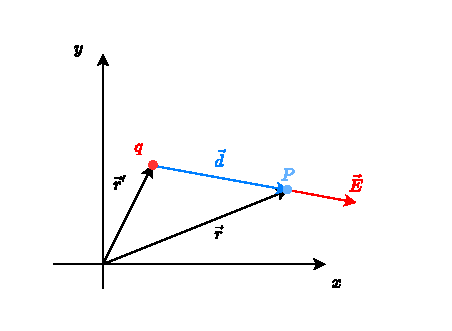
\includegraphics[width=0.7\linewidth]{res/svg/point_charge.drawio}
  \caption{Point charge in space}
\end{figure}
We want to calculate the potential and the electric field at a point $\vec{r}$. The potential only depends on the distance between the points which we will denote with the vector $\vec{d}$. Actually the potential only depends on the modulus of the distance which is $d = \norm{\vec{r}-\vec{r}'}$. Instead, the electric field is given by Coulomb's law:
\begin{equation}
  \vec{E}(\vec{r}) = \dfrac{1}{4 \pi \epsz}\dfrac{Q}{\norm{\vec{r}-\vec{r}'}^3}\brackets{\vec{r}-\vec{r}'}
\end{equation}
We could define a radial versor $\hat{u}_r \defineeq \dfrac{\vec{r}-\vec{r}'}{\norm{\vec{r}-\vec{r}'}}$, but this would be essentially useless, instead with the given notation we do not need to account for extra stuff during calculations.\\
Now, instead of a single point charge, we imagine putting $n$ charges in space, and we still want to evaluate the electric field at $\vec{r}$. To do this we simply add (vectorially) all the contributions of the charges:
\begin{equation}
  \vec{E}(\vec{r}) = \bigsum_i\dfrac{1}{4 \pi \epsz}\dfrac{Q_i}{\norm{\vec{r}-\vec{r}_i'}^3}\brackets{\vec{r}-\vec{r}_i'}
\end{equation}
Same goes for the potential:
\begin{equation}
  \potE(\vec{r}) = \bigsum_i\dfrac{1}{4 \pi \epsz}\dfrac{Q_i}{\norm{\vec{r}-\vec{r}_i'}}
\end{equation}
If instead of a finite number of point charges we are dealing with a continuous distribution of charges we simply ``switch'' the discrete summation with an integral and integrate over all charges:
\begin{equation}
  \potE(\vec{r}) = \dfrac{1}{4 \pi \epsz}\int_Q \dfrac{\dd{q}}{\norm{\vec{r}-\vec{r}'}}
\end{equation}
The infinitesimal element $\dd{q}$ just represents the charge of an infinitesimal volume $\dd{\tau}$ and so, given the distribution's density we can say that $\dd{q} = \rho \dd{\tau} = \rho \dd{^3 \vec{r}}$, but we need to remind that we are now integrating over a volume. So the new formula becomes:
\begin{equation} \label{e:general_sol_poisson}
  \potE(\vec{r}) = \dfrac{1}{4 \pi \epsz}\int_{\tau} \dfrac{\rho (\vec{r}')}{\norm{\vec{r}-\vec{r}'}}\dd{^3 \vec{r}}
\end{equation}
There is another immediate property of the potential $\potE$. If we simply substitute $-\grad{\potE}$ in the first Maxwell equation we get:
\begin{equation}
  \div{\vec{E}} = \div{\brackets{-\grad{\potE}}} = -\lap{\potE} = \dfrac{\rho}{\epsz}
\end{equation}
The last equation can be simply rewritten as:
\begin{equation} \label{e:Poisson_eq}
  \boxed{\lap{\potE} = -\dfrac{\rho}{\epsz}}
\end{equation}
Which is called \textbf{Poisson's equation}. We can do a similar thing for the vector potential $\vec{A}$. We recall that this property is true:
\begin{equation}
  \curl{(\curl{\vec{C}})} = \grad{(\div{\vec{C}})} - \lap{\vec{C}}
\end{equation}
The laplacian operator, in this case, is inteded as applied to every component of $\vec{C}$. To apply this to the vector potential we simply substitute $\vec{B} = \curl{\vec{A}}$ in the fourth Maxwell equation (stationary case):
\begin{equation}
  \grad{(\div{\vec{A}})} - \lap{\vec{A}} = \muz \vec{J}
\end{equation}
And so finally we arrived to this set of equation:
\begin{equation} \label{e:pot_stat_eq}
  \begin{split}
    &\lap{\potE} = -\dfrac{\rho}{\epsz}\\[8pt]
    &\grad{(\div{\vec{A}})} - \lap{\vec{A}} = \muz \vec{J}
  \end{split}
\end{equation}
Which is a set of 4 equations (1 for $\potE$, 3 for $\vec{A}$) which are completely equivalent to \maxwellref\;in the stationary case, since we derived them from \maxwellref\;themselves.\\
Let's continue with the non-stationary case. The divergence of $\vec{B}$ will still be:
\begin{equation}
  \div{\vec{B}} = 0
\end{equation}
Thus, we can still define a vector potential in the same way we did for the stationary case:
\begin{equation}
  \vec{B} = \curl{\vec{A}}
\end{equation}
But looking at the third \maxwellref\;we get:
\begin{equation}
  \curl{\vec{E}} = -\pdv{}{t}\curl{\vec{A}}
\end{equation}
And so the field $\vec{E}$ itself is not irrotational anymore. Instead, if we bring all the terms to one side we have:
\begin{equation}
  \curl{\brackets{\vec{E} + \pdv{\vec{A}}{t}}} = 0
\end{equation}
And so $\vec{E} + \pdv{\vec{A}}{t}$ is irrotational. We can thus define a new scalar potential with the form:
\begin{equation}
  -\grad{\potE} = \vec{E} + \pdv{\vec{A}}{t}
\end{equation}
And so the electric field $\vec{E}$ will now be:
\begin{equation}
  \vec{E} =  -\grad{\potE} -\pdv{\vec{A}}{t}
\end{equation}
So the first Maxwell equation becomes:
\begin{equation}
  \begin{split}
    \div{\vec{E}} &= \div{\brackets{-\grad{\potE} -\pdv{\vec{A}}{t}}} = \\[8pt]
    &= \boxed{-\lap{\potE} -\pdv{}{t}\div{\vec{A}} = \dfrac{\rho}{\epsz}}
  \end{split}
\end{equation}
The fourth Maxwell equation will now simply be:
\begin{equation}
  \boxed{\grad{\brackets{\div{\vec{A}}}} - \lap{\vec{A}} = \muz \vec{J} + \muz \epsz \pdv{}{t}\brackets{-\grad{\potE} - \pdv{\vec{A}}{t}}}
\end{equation}
\section{Gauge transformations}
In this section we will introduce a type of transformation which will help us to achieve a more compact and elegant way to write \maxwellref.
\begin{definition}{Gauge transformations}
  Gauge transformations are transformations of the potentials that leave the fields unchanged.
\end{definition}
\noindent In the static case a simple gauge transformation for the electric field can be:
\begin{equation}
  \begin{split}
    &\potE \longrightarrow \potE' = \potE + c\\[8pt]
    \implies &-\grad{\potE'} = -\grad{\brackets{\potE + c}} = -\grad{\potE} - \cancel{\grad{c}} = -\grad{\potE} = \vec{E}\\[8pt]
    &-\grad{\potE'} = \vec{E}
  \end{split}
\end{equation}
Obviously the field $\vec{E}$ remains the same since the gradient of a function is invariant under translation of that function. Similarly, we can do a simple transformation for the potential vector:
\begin{equation}
  \begin{split}
    &\vec{A} \longrightarrow \vec{A}' = \vec{A} + \grad{\xi}\\[8pt]
    \implies &\curl{\vec{A}'} = \curl{\brackets{\vec{A} + \grad{\xi}}} = \curl{\vec{A}} + \cancel{\curl{\grad{\xi}}} = \curl{\vec{A}} = \vec{B}\\[8pt]
    &\curl{\vec{A}'} = \vec{B}
  \end{split}
\end{equation}
Where the function $\xi (\vec{x})$ is called \textbf{Gauge function} and is a function of only the coordinates. As we anticipated we can exploit those transformations to simplify the equations we previously got. In particular if we make a gauge transformation such that:
\begin{equation}
  \div{\vec{A}'} = 0
\end{equation}
Then the second equation in \eqref{e:pot_stat_eq} becomes:
\begin{equation}
  \begin{split}
    \grad{(\cancel{\div{\vec{A}'}})} - \lap{\vec{A}'} &= \muz \vec{J}\\[8pt]
    \lap{\vec{A}'} &= -\muz \vec{J}
  \end{split}
\end{equation}
This transformation is thus defined as:
\begin{definition}{Coulomb gauge}
  The Coulomb gauge is a transformation such that:
  \begin{equation}
    \div{\vec{A}'} = 0
  \end{equation}
\end{definition}
\noindent In order to be able to perform this transformation we need to choose a proper functional form of $\xi$. By using the definition we have:
\begin{equation}
  \begin{split}
    &\div{\brackets{\vec{A}+\grad{\xi}}} \overset{!}{=} 0 \\[8pt]
    &\div{\vec{A}} + \lap{\xi} = 0 \\[8pt]
    &\boxed{\lap{\xi} = -\div{\vec{A}}}
  \end{split}
\end{equation}
So this is the condition that $\xi$ must obey in order to generate the Coulomb gauge. Obviously we can make another transformation in the Coulomb gauge that remanis in the Coulomb gauge. Repeating the steps we did for the general condition we get:
\begin{equation}
  \begin{split}
    &\div{\brackets{\vec{A}'+\grad{\xi'}}} \overset{!}{=} 0 \\[8pt]
    &\cancel{\div{\vec{A}'}} + \lap{\xi'} = 0 \\[8pt]
    &\lap{\xi'} = 0
  \end{split}
\end{equation}
This means that the function must be harmonic.\\
In conclusion, for the stationary case we can sum up the equations of the potential in the Coulomb gauge in a single form:
\begin{equation}
  \lap{\psi} = -s
\end{equation}
Where:
\begin{itemize}
  \item $\psi$ is the potential, either $\potE$ or a component $A_i$
  \item $s$ is the source of the field, either $\rho/\epsz$ or $\muz J_i$
\end{itemize}
Now let's move on to the general case (non-stationary case). We can still start from the basic transformation for the vector potential, but in this case we get:
\begin{equation}
  \begin{split}
    \vec{E} &\overset{!}{=} -\grad{\potE'} - \pdv{\vec{A'}}{t} \\[8pt]
    -\grad{\potE} - \cancel{\pdv{\vec{A}}{t}} &= -\grad{\potE'} - \pdv{}{t}\brackets{\cancel{\vec{A}} + \grad{\xi}} \\[8pt]
    \grad{\potE} &= \grad{\potE'} + \pdv{}{t}\brackets{\grad{\xi}} \\[8pt]
    \potE' &= \potE - \pdv{\xi}{t}
  \end{split}
\end{equation}
So this is the second ``basic transformation'' in the general case. Keep in mind that we are looking for a way to further simplify these equations:
\begin{equation}
  \begin{split}
    &-\lap{\potE} -\pdv{}{t}\div{\vec{A}} = \dfrac{\rho}{\epsz} \\[8pt]
    &\grad{\brackets{\div{\vec{A}}+ \dfrac{1}{c^2}\pdv{\potE}{t}}} - \lap{\vec{A}} + \dfrac{1}{c^2} \pdv[2]{\vec{A}}{t} = \muz \vec{J}
  \end{split}
\end{equation}
We define a new transformation:
\begin{definition}{Lorenz gauge}
  The Lorenz gauge is a gauge transformation such that:
  \begin{equation} \label{e:Lorentz_gauge}
    \div{\vec{A}'}+ \dfrac{1}{c^2}\pdv{\potE'}{t} = 0
  \end{equation}
\end{definition}
If we succed in finding this transformation the second equations then become:
\begin{equation}
  \begin{split}
    &\lap{\potE'} - \dfrac{1}{c^2} \pdv[2]{\potE'}{t} = -\dfrac{\rho}{\epsz} \\[8pt]
    &\lap{\vec{A}'} - \dfrac{1}{c^2} \pdv[2]{\vec{A}'}{t} = -\muz \vec{J}
  \end{split}
\end{equation}
We can easily spot the simmetry of those equations. In particular, we now define a new operator:
\begin{definition}{D'Alembert operator}
  The D'Alembert operator is an operator constructed as follows:
  \begin{equation}
    \dalop \defineeq \lap - \dfrac{1}{c^2} \pdv[2]{}{t}
  \end{equation}
\end{definition}
And so the equations can be rewritten as:
\begin{equation}
  \begin{split}
    &\dalop \potE' = -\dfrac{\rho}{\epsz} \\[8pt]
    &\dalop \vec{A}' = -\muz \vec{J}
  \end{split}
\end{equation}
We still need to understand if this transformation is possible. Recall that the possible basic transformations in this case are:
\begin{equation}
  \begin{split}
    &\potE \longrightarrow \potE' = \potE - \pdv{\xi}{t}\\[8pt]
    &\vec{A} \longrightarrow \vec{A}' = \vec{A} + \grad{\xi}
  \end{split}
\end{equation}
And we want to achieve \eqref{e:Lorentz_gauge}. By substituting we get:
\begin{equation}
  \begin{split}
    &\div{\brackets{\vec{A} + \grad{\xi}}} + \dfrac{1}{c^2} \pdv{}{t}\brackets{\potE - \pdv{\xi}{t}} = 0 \\[8pt]
    &\div{\vec{A}} + \lap{\xi} + \dfrac{1}{c^2} \pdv{\potE}{t} - \dfrac{1}{c^2} \pdv[2]{\xi}{t} = 0 \\[8pt]
    &\lap{\xi} - \dfrac{1}{c^2} \pdv[2]{\xi}{t} = -\div{\vec{A}} - \dfrac{1}{c^2} \pdv{\potE}{t} \\[8pt]
    &\boxed{\dalop \xi = -\brackets{\div{\vec{A}} + \dfrac{1}{c^2} \pdv{\potE}{t}}}
  \end{split}
\end{equation}
As for the Coulomb gauge we can make a transformation in the Lorenz gauge and stay in the Lorenz gauge. Similarly to what we got before the condition for the new gauge function will be:
\begin{equation}
  \dalop \xi' = 0
\end{equation}
\section{Solutions to the potential equations}
Now that we have the equations for the potentials in a more compact way we can ask ourselves what the solutions to those equations are. We already know that the most general solution for $\potE$ \underline{in the static case} is:
\begin{equation}
  \potE(\vec{r}) = \dfrac{1}{4 \pi \epsz}\int_{\tau} \dfrac{\rho (\vec{r}')}{\norm{\vec{r}-\vec{r}'}}\dd{^3 \vec{r}}
\end{equation}
Not so surprisingly the solution for each component of $\vec{A}$ will be something very similar to this solution. In particular, it will be:
\begin{equation}
  A_i(\vec{r}) = \dfrac{\muz}{4 \pi }\int_{\tau} \dfrac{J_i}{\norm{\vec{r}-\vec{r}'}}\dd{^3 \vec{r}}
\end{equation}
And so we can write the solutions in the compact form:
\begin{equation} \label{e:pot_general_solutions}
  \begin{split}
    &\potE(\vec{r}) = \dfrac{1}{4 \pi \epsz}\int_{\tau} \dfrac{\rho (\vec{r}')}{\norm{\vec{r}-\vec{r}'}}\dd{^3 \vec{r}} \\[8pt]
    &\vec{A}(\vec{r}) = \dfrac{\muz}{4 \pi }\int_{\tau} \dfrac{\vec{J} (\vec{r}')}{\norm{\vec{r}-\vec{r}'}}\dd{^3 \vec{r}}
  \end{split}
\end{equation}
Actually the volume element in the second equation is just the volume of the cable where the current generating the field is passing thus it can be explicited as:
\begin{equation}
  \dd{\tau} = \Sigma \dd{l}
\end{equation}
\begin{figure}[H]
  \centering
  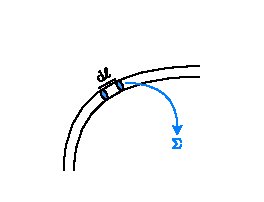
\includegraphics[width=0.5\linewidth]{res/svg/cable.drawio}
  \caption{Wire element}
\end{figure}
Since $J\Sigma = i$ if we ``pass'' the unit vector of $\vec{J}$ to the infinitesimal length element we obtain an integration of the current only over the circuit:
\begin{equation}
  \vec{A}(\vec{r}) = \dfrac{\muz}{4 \pi }\int_{\gamma} \dfrac{i \dd{\vec{l}}}{\norm{\vec{r}-\vec{r}'}}
\end{equation}
Now we want to prove that the general solution stated in \eqref{e:pot_general_solutions} is indeed a solution. We simply verify that $\vec{B} = \curl{\vec{A}}$:
\begin{equation}
  \begin{split}
    \curl{\vec{A}} &= \curl \dfrac{\muz}{4 \pi }\int_{\tau} \dfrac{\vec{J} (\vec{r}')}{\norm{\vec{r}-\vec{r}'}}\dd{^3 \vec{r}} \\[8pt]
    &=  \dfrac{\muz}{4 \pi }\int_{\tau} \curl{\brackets{\dfrac{\vec{J} (\vec{r}')}{\norm{\vec{r}-\vec{r}'}}}} \dd{^3 \vec{r}}
  \end{split}
\end{equation}
Now we need to exploit this identity:
\begin{equation}
  \curl{\brackets{\vec{f}g}} = g\curl{\vec{f}} + \grad{g} \cross \vec{f}
\end{equation}
In our equation this will result in:
\begin{equation}
  \begin{split}
    &\dfrac{\muz}{4 \pi }\int_{\tau} \curl{\brackets{\dfrac{\vec{J} (\vec{r}')}{\norm{\vec{r}-\vec{r}'}}}} \dd{^3 \vec{r}} = \\[8pt]
    &= \dfrac{\muz}{4 \pi }\int_{\tau}\sqbr{ \cancel{\curl{\brackets{\vec{J}(\vec{r}')}}}\dfrac{1}{\norm{\vec{r}-\vec{r}'}}  + \grad{\brackets{\dfrac{1}{\norm{\vec{r}-\vec{r}'}}}} \cross \vec{J}(\vec{r}')}\dd{^3 \vec{r}}
  \end{split}
\end{equation}
The curl of $\vec{J}$ is zero since it does not depend on the coordinates $x,y,z$ of the gradient. For the gradient of the norm of the distance we just explicit the calculation. For the partial derivative with respect to $x$ we have:
\begin{equation}
  \begin{split}
    \pdv{}{x}\brackets{\dfrac{1}{\sqrt{(x-x')^2 + (y-y')^2 + (z-z')^2}}} = -\dfrac{\cancel{2}(x-x')}{\cancel{2}\sqbr{(x-x')^2 + (y-y')^2 + (z-z')^2}^{3/2}}
  \end{split}
\end{equation}
The result will be essentially the same for the other components thus the integral now becomes:
\begin{equation}
  \dfrac{\muz}{4 \pi }\int_{\tau}-\brackets{\dfrac{\vec{r}-\vec{r}'}{\norm{\vec{r}-\vec{r}'}^3}} \cross \vec{J}(\vec{r}')\dd{^3 \vec{r}}
\end{equation}
If we switch the order of the cross product we must change sign, also we can apply the trick we explained before to integrate over the circuit, and so we end up with:
\begin{equation}
  \dfrac{\muz}{4 \pi }\int_{\gamma}\dfrac{i \dd{\vec{l}} \cross \brackets{\vec{r}-\vec{r}'}}{\norm{\vec{r}-\vec{r}'}^3}
\end{equation}
Now we want to find a general solution for the \underline{non-stationary} case of the potential equations. Our problem is solved if we find a general solution to this equation:
\begin{equation}
  \dalop \psi = -s
\end{equation}
Then we can easily adapt it to the different sources and potentials we can possibly have. Now imagine being far from the source, in this case the contirbution of $s$ goes to zero, and we have:
\begin{equation}
  \dalop \psi = 0
\end{equation}
Which is just the D'Alembert equation. Suppose that we have a single spherical source in the origin and we want to calculate the potential $\psi (P)$ in a point $P$ very far from the source.
\begin{figure}[H]
  \centering
  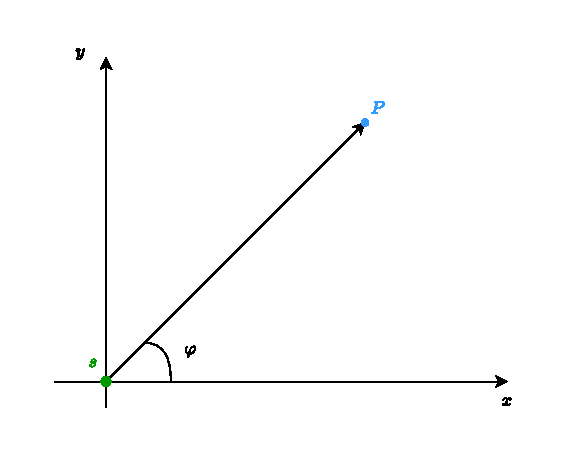
\includegraphics[width=0.7\linewidth]{res/svg/long_distance_potential.drawio}
  \caption{Long distance potential}
\end{figure}
Since we are considering a spherical simmetry we should use D'Alembert in spherical coordinates. We just need to change the laplacian which can be written as:
\begin{equation}
  \lap = \dfrac{1}{r^2} \pdv{}{r}\bbrackets{r^2 \pdv{}{r}} + \dfrac{1}{r^2 \sin{\theta}} \pdv{}{\theta}\bbrackets{\sin{\theta} \pdv{}{\theta}} + \dfrac{1}{r^2 \sin^2{\theta}} \pdv[2]{}{\varphi}
\end{equation}
Since in our case there is no dependence on $\theta$ or $\varphi$ the D'Alembert operator applied to $\psi$ results in:
\begin{equation} \label{e:dalop_far_source}
  \dalop \psi = \dfrac{1}{r^2} \pdv{}{r}\bbrackets{r^2 \pdv{\psi}{r}} - \dfrac{1}{c^2} \pdv[2]{\psi}{t} = 0
\end{equation}
Let's evaluate the first term:
\begin{equation}
  \dfrac{1}{r^2} \pdv{}{r}\bbrackets{r^2 \pdv{\psi}{r}} = \dfrac{1}{r^2} \sqbr{2r \pdv{\psi}{r} + r^2 \pdv[2]{\psi}{r}} = \dfrac{2}{r} \pdv{\psi}{r} + \pdv[2]{\psi}{r}
\end{equation}
Which can also be seen as:
\begin{equation}
  \begin{split}
    &\dfrac{1}{r} \pdv{\psi}{r} + \dfrac{1}{r} \pdv{\psi}{r} + \pdv[2]{\psi}{r} = \dfrac{1}{r} \pdv{\psi}{r} + \dfrac{1}{r}\pdv{}{r}\brackets{r\pdv{\psi}{r}} = \\[8pt]
    &= \dfrac{1}{r} \pdv{}{r}\brackets{\psi + r\pdv{\psi}{r}} = \dfrac{1}{r}\pdv{}{r}\brackets{\pdv{\brackets{r\psi}}{r}} = \dfrac{1}{r}\pdv[2]{\brackets{r\psi}}{r}
  \end{split}
\end{equation}
And so \eqref{e:dalop_far_source} can be rewritten as:
\begin{equation}
  \pdv[2]{\brackets{r\psi}}{r} - \dfrac{1}{c^2} \pdv[2]{\brackets{r\psi}}{t} = 0
\end{equation}
Which means that $r\psi$ is a plane wave, but we don't know the actual solution. In general, we know that:
\begin{equation}
  r\psi = f^+(r+ct) + f^-(r-ct)
\end{equation}
We can exclude the first function $f(r+ct)$ since it has no physical meaning (it would be a wave going from infinity to the source). And so $\psi$ becomes:
\begin{equation}
  \psi = \dfrac{1}{r} f(r-ct)
\end{equation}
Which is the equation of a spherical wave and can also be written as:
\begin{equation}
  \boxed{\psi(r,t) = \dfrac{1}{r} f(kr - \omega t)}
\end{equation}
To solve the original equation we impose the boundary conditions:
\begin{equation}
  s(r,t) = S(t)\delta^3(r)
\end{equation}
This is precisely the expression for a time varying point charge in the origin. By the definition of the Dirac delta function we know that outside the origin $s=0$ and so the solution is what we previously got:
\begin{equation}
  \psi(r,t) = \dfrac{1}{r} f(kr - \omega t) = \dfrac{1}{r} f\brackets{-\omega\brackets{t- \dfrac{k}{\omega}r}} = \dfrac{1}{r}g\brackets{t - \dfrac{r}{c}}
\end{equation}
The term $\dfrac{r}{c}$ is the \textbf{retarded time} which is the cause of delay effects in the action of the potential. If a change occurs at time $t$ its effect will be seen at a distance $r$ only at time $t + \dfrac{r}{c}$. This term is only negligible if we are considering a distance $r$ such that $\abs{r} \ll \abs{c}$.
Now we can substitute $\psi$ into the orginal equation. For the laplacian in spherical coordinates we first calculate the gradient:
\begin{equation}
  \begin{split}
    &\pdv{}{r}\sqbr{\dfrac{1}{r}g\brackets{t - \dfrac{r}{c}}}\hat{u}_r =\\[8pt]
    &= -\dfrac{1}{r^2}g\brackets{t - \dfrac{r}{c}}\hat{u}_r + \dfrac{1}{r}\pdv{g}{\brackets{t - \dfrac{r}{c}}}\pdv{\brackets{t - \dfrac{r}{c}}}{r}\hat{u}_r =\\[8pt]
    &= \sqbr{-\dfrac{1}{r^2}g + \dfrac{1}{r}\brackets{- \dfrac{1}{c}}g'}\hat{u}_r
  \end{split}
\end{equation}
For the time derivative we have:
\begin{equation}
  \begin{split}
    &\pdv{}{t}\sqbr{\dfrac{1}{r}g\brackets{t - \dfrac{r}{c}}} =\\[8pt]
    &= \dfrac{1}{r}\pdv{g}{\brackets{t - \dfrac{r}{c}}}\pdv{\brackets{t - \dfrac{r}{c}}}{t} =\\[8pt]
    &=\dfrac{1}{r}g'
  \end{split}
\end{equation}
Similarly the second time derivative will result in:
\begin{equation}
  \pdv[2]{g}{t} = \dfrac{1}{r}g''
\end{equation}
And so the equation will be:
\begin{equation}
  \div{\sqbr{-\dfrac{1}{r^2}g + \dfrac{1}{r}\brackets{- \dfrac{1}{c}}g'}}\hat{u}_r - \dfrac{1}{c^2}\dfrac{1}{r}g'' = -S(t)\delta^3(r)
\end{equation}
Let's now integrate this equation with respect to $\dd{^3\vec{r}}$.
The right side is easy since:
\begin{equation}
  -\int_{\Omega} S(t)\delta^3(r) \dd{^3 r} = -S(t)
\end{equation}
The left side will be:
\begin{equation}
  \int_{\Omega} \div{\sqbr{-\dfrac{1}{r^2}g + \dfrac{1}{r}\brackets{- \dfrac{1}{c}}g'}}\hat{u}_r \dd{^3\vec{r}} - \int_{\Omega}\dfrac{1}{c^2}\dfrac{1}{r}g''\dd{^3\vec{r}}
\end{equation}
For the first term we can apply the divergence theorem, for the second we can rewrite the differential as $\dd{^3\vec{r}} = 4\pi r^2 \dd{r}$ by using the spherical change of coordinates:
\begin{equation}
  \int_{\partial \Omega} \sqbr{-\dfrac{1}{r^2}g + \dfrac{1}{r}\brackets{- \dfrac{1}{c}}g'} \underbrace{\hat{u}_r \cdot \hat{u}_n}_{=\;1} \dd{\Sigma} - \int_{\Omega}\dfrac{1}{c^2}\dfrac{1}{r}g''4\pi r^2 \dd{r}
\end{equation}
For a generic spherical volume of radius $R$, the surface will be $4\pi R^2$ and so the first term will be:
\begin{equation}
  -4\pi g - \dfrac{4 \pi}{c}g'R
\end{equation}
Taking the limit as $R \rightarrow 0$ the only surviving terms will be:
\begin{equation}
  -4\pi g = -S(t)
\end{equation}
Since $g'R$ goes to zero and also the integral of the time dependent part goes to zero. So g will be:
\begin{equation}
  g(t) = \dfrac{S(t)}{4\pi}
\end{equation}
Finally our solution must take into account the delay effect:
\begin{equation}
  \psi\brackets{r,t} = \dfrac{1}{r}g\brackets{t-\dfrac{r}{c}}= \dfrac{S\brackets{t-\dfrac{r}{c}}}{4\pi r}
\end{equation}
For example if $S(t) = S_0\sin\brackets{\omega t}$, $\psi$ will be:
\begin{equation}
  \psi\brackets{r,t} = \dfrac{S_0}{4\pi r}\sin \sqbr{\omega\brackets{t-\dfrac{r}{c}}} = \dfrac{S_0}{4\pi r}\sin \brackets{\omega t- kr}
\end{equation}
If the source is not at the origin but in a generic point $\vec{r}'$ we just need to shift our solution:
\begin{equation}
  \psi\brackets{\vec{r},t} = \dfrac{1}{4\pi}\dfrac{S\brackets{\vec{r}', t-\frac{\norm{\vec{r}-\vec{r}'}}{c}}}{\norm{\vec{r}-\vec{r}'}}
\end{equation}
In the case of a distribution of charges we need to integrate over the volume that contains the charges:
\begin{equation}
  \psi\brackets{\vec{r},t} = \dfrac{1}{4\pi}\int_{\Omega }\dfrac{S\brackets{\vec{r}', t-\frac{\norm{\vec{r}-\vec{r}'}}{c}}}{ \norm{\vec{r}-\vec{r}'}} \dd{\vec{r}}
\end{equation}
This is precisely the form we anticipated for the general form of the potentials. In particular, by substituting the different cases of $\psi$ and $S$ we arrive to:
\begin{equation}
  \begin{split}
    &\potE(\vec{r},t) = \dfrac{1}{4 \pi \epsz}\int_{\tau} \dfrac{\rho \brackets{\vec{r}', t-\frac{\norm{\vec{r}-\vec{r}'}}{c}}}{\norm{\vec{r}-\vec{r}'}}\dd{^3 \vec{r}} \\[8pt]
    &\vec{A}(\vec{r},t) = \dfrac{\muz}{4 \pi }\int_{\tau} \dfrac{\vec{J} \brackets{\vec{r}', t-\frac{\norm{\vec{r}-\vec{r}'}}{c}}}{\norm{\vec{r}-\vec{r}'}}\dd{^3 \vec{r}}
  \end{split}
\end{equation}
\chapter[EM and mechanics]{Electromagnetism and analytical mechanics}
\section{The generalized potential}
Now we want to find a connection between what we studied in analytical mechanics and Electromagnetism. Let's start from \lagrangeref :
\begin{equation}
  \dv{}{t}\pdv{T}{\dot{q}_{\alpha}} -\pdv{T}{q_{\alpha}} = Q_{\alpha}
\end{equation}
If the forces can be expressed as the gradient of a potential $\vec{F}_i = -\grad_i V$ then:
\begin{equation}
  Q_{\alpha} = \bigsum_i \vec{F}_i \cdot \pdv{\vec{r}_i}{q_{\alpha}} = \bigsum_i \brackets{-\grad_i V} \cdot \pdv{\vec{r}_i}{q_{\alpha}} = -\pdv{V}{q_{\alpha}}
\end{equation}
If $V$ does not depend on the velocities we can arrive to \eleref :
\begin{equation}
  \dv{}{t}\pdv{\lagr}{\dot{q}_{\alpha}} - \pdv{\lagr}{q_{\alpha}} = 0
\end{equation}
We also stated that sometimes it's possible to derive a generalized version of the \eleref\;if there exists a generalized potential $\mu$ such that:
\begin{equation}
  Q_{\alpha} = -\pdv{\mu}{q_{\alpha}} + \dv{}{t}\pdv{\mu}{\dot{q}_{\alpha}}
\end{equation}
If this is possible we define the generalized Lagrangian as:
\begin{equation}
  \lagr = T - \mu
\end{equation}
and we arrive at the same equations we previously got.\\
This was already known in the study of analytical mechanics, the new thing is that the generalized potential can be defined for the Lorentz force:
\begin{equation}
  \vec{F} = q (\vec{E} + \vec{v} \cross \vec{B})
\end{equation}
Let's imagine a simple system constituted by a single unconstrained particle of mass $m$ and charge $q$ in an electromagnetic field. This means that the only force acting on the particle is the Lorentz force. Since the particle is unconstrained we can use cartesian coordinates. For the $x$ component of $Q$ we have:
\begin{equation}
  Q_x = \vec{F} \cdot \pdv{\vec{r}}{x} = F_x
\end{equation}
And so:
\begin{equation}
  Q_x = F_x = q (E_x + \brackets{\vec{v} \cross \vec{B}}_x)
\end{equation}
By substituting the potential equations we have:
\begin{equation} \label{e:LorentzF_x}
  F_x = q \brackets{-\pdv{\potE}{x} - \pdv{A_x}{t} + \brackets{\vec{v} \cross \curl{\vec{A}}}_x}
\end{equation}
Let's first evaluate $\curl{\vec{A}}$:
\begin{equation}
  \curl{\vec{A}} =
  \begin{vmatrix}
  \hat{u}_x & \hat{u}_y & \hat{u}_z \\
  \pdv{}{x} & \pdv{}{y} & \pdv{}{z} \\
  A_x & A_y & A_z
  \end{vmatrix}
  = \bbrackets{\pdv{A_z}{y} - \pdv{A_y}{z}}\hat{u}_x
  + \bbrackets{\pdv{A_x}{z} - \pdv{A_z}{x}}\hat{u}_y
  + \bbrackets{\pdv{A_y}{x} - \pdv{A_x}{y}}\hat{u}_z
\end{equation}
Now we do the cross product of $v$ and $\curl{\vec{A}}$:
\begin{equation}
  \begin{split}
    &\begin{vmatrix}
      \hat{u}_x & \hat{u}_y & \hat{u}_z \\
      v_x & v_y & v_z \\
      \bbrackets{\pdv{A_z}{y} - \pdv{A_y}{z}} & \bbrackets{\pdv{A_x}{z} - \pdv{A_z}{x}} & \bbrackets{\pdv{A_y}{x} - \pdv{A_x}{y}}
    \end{vmatrix}
    = \\[8pt]
      &= \sqbr{v_y \bbrackets{\pdv{A_y}{x} - \pdv{A_x}{y}} - v_z \bbrackets{\pdv{A_x}{z} - \pdv{A_z}{x}}}\hat{u}_x +\\[8pt]
      &+ \sqbr{v_z \bbrackets{\pdv{A_z}{y} - \pdv{A_y}{z}} - v_x \bbrackets{\pdv{A_y}{x} - \pdv{A_x}{y}}}\hat{u}_y +\\[8pt]
      &+ \sqbr{v_x \bbrackets{\pdv{A_x}{z} - \pdv{A_z}{x}} - v_y \bbrackets{\pdv{A_z}{y} - \pdv{A_y}{z}}}\hat{u}_z
  \end{split}
\end{equation}
And so \eqref{e:LorentzF_x} will now be:
\begin{equation}
  F_x = q \brackets{-\pdv{\potE}{x} - \pdv{A_x}{t} + v_y \pdv{A_y}{x} - v_y\pdv{A_x}{y} - v_z \pdv{A_x}{z} - v_z\pdv{A_z}{x}}
\end{equation}
Now we add and subtract the term $v_x \pdv{A_x}{x}$:
\begin{equation}
  F_x = q \bigg(-\pdv{\potE}{x} - \pdv{A_x}{t} + \underbrace{v_x \pdv{A_x}{x} + v_y \pdv{A_y}{x} + v_z\pdv{A_z}{x}}_{\vec{v}\cdot \frac{\partial \vec{A}}{\partial x}} \underbrace{- v_x \pdv{A_x}{x}- v_y\pdv{A_x}{y} - v_z \pdv{A_x}{z}}_{-\vec{v} \cdot \grad{A_x}} \bigg)
\end{equation}
And so $F_x$ will be:
\begin{equation}
  \begin{split}
    &q \brackets{-\pdv{\potE}{x} - \pdv{A_x}{t}  -\vec{v} \cdot \grad{A_x} + \vec{v}\cdot \pdv{\vec{A}}{x}} = \\[8pt]
    &= q \brackets{-\pdv{\potE}{x} - \dv{A_x}{t} + \vec{v}\cdot \pdv{\vec{A}}{x}} = \\[8pt]
    &= -\pdv{}{x}\sqbr{q\brackets{\potE - \vec{v}\cdot \vec{A}}} - \dv{}{t}\brackets{qA_x}
  \end{split}
\end{equation}
We could then reasonably think that $\mu = q\brackets{\potE - \vec{v}\cdot \vec{A}}$ might be our generalized potential. To verify this let's evaluate the partial derivative with respect to $\dot{x}$:
\begin{equation}
  \begin{split}
    \pdv{}{\dot{x}} \sqbr{q\brackets{\potE - \vec{v}\cdot \vec{A}}} &= -q \pdv{}{\dot{x}} \sqbr{\vec{v} \cdot \vec{A}} = \\[8pt]
    &= -q \pdv{}{\dot{x}} \sqbr{\dot{x} A_x + \dot{y} A_y + \dot{z} A_z} = -q A_x
  \end{split}
\end{equation}
And so we verified that for $\mu$ the condition for the generalized potential holds. Obviously the same should be done for every component, but the calculations will be the same.\\
Now we can notice that $\mu$ is not gauge invariant. If we apply the gauge transformation:
\begin{equation}
  \begin{split}
    &\potE \longrightarrow \potE' = \potE - \pdv{\xi}{t} \\[8pt]
    &\vec{A} \longrightarrow \vec{A}' = \vec{A} + \grad{\xi}
  \end{split}
\end{equation}
We get that:
\begin{equation}
  \mu' = q\brackets{\potE  - \vec{v}\cdot \vec{A} - \pdv{\xi}{t} - \vec{v}\cdot \grad{\xi}} = q\brackets{\potE  - \vec{v}\cdot \vec{A} -\dv{\xi}{t}} = \mu -\dv{\brackets{q\xi}}{t}
\end{equation}
What happens instead for the Lagrangian? We simply substitute:
\begin{equation} \label{e:gauge_lagr}
  \tilde{\lagr} = T - \mu' = T -\mu +\dv{\brackets{q\xi}}{t} = \lagr  +\dv{\brackets{q\xi}}{t}
\end{equation}
This is the equation we would expect if $q\xi$ was a generating function of a canonical transformation and we will further discuss this later.\\
Now let's go back to the original Lagrangian:
\begin{equation}
  \lagr = T - \mu = \dfrac{1}{2}mv^2 - q\brackets{\potE - \vec{v} \cdot \vec{A}}
\end{equation}
The momentum conjugated to $x$ (and similarly for the other coordinates) is:
\begin{equation}
  \begin{split}
    \pdv{\lagr}{\dot{x}} &= \pdv{}{\dot{x}}\sqbr{\dfrac{1}{2}m\brackets{\dot{x}^2 + \dot{y}^2 + \dot{z}^2} - q\potE + q\brackets{\dot{x} \hat{u}_x + \dot{y} \hat{u}_y + \dot{z} \hat{u}_z} \cdot \vec{A}} =\\[8pt]
    &= m\dot{x} + q\hat{u}_x \cdot \vec{A} = m\dot{x} + qA_x
  \end{split}
\end{equation}
Thus:
\begin{equation}
  \vec{p} = m\vec{v} + q\vec{A}
\end{equation}
And so $\vec{p}$ is not the total linear momentum and is not gauge invariant but, using \eleref :
\begin{equation}
  \begin{split}
    &\dv{p_x}{t} - \pdv{\lagr}{x} = 0\\
    &\dv{}{t}\brackets{m\dot{x} + qA_x} - \pdv{}{x}\brackets{\dfrac{1}{2}mv^2 - q\brackets{\potE - \vec{v} \cdot \vec{A}}} = 0\\[8pt]
    &m\ddot{x} +q\dv{A_x}{t} + q\pdv{\potE}{x} - \pdv{}{x}\brackets{\vec{v} \cdot \vec{A}} = 0\\[8pt]
    &m\ddot{x} = \underbrace{-q\dv{A_x}{t} - q\pdv{\potE}{x} + \pdv{}{x}\brackets{\vec{v} \cdot \vec{A}}}_{F_x}\\[8pt]
    &m\ddot{x} = F_x
  \end{split}
\end{equation}
Finally, we can express the total force as:
\begin{equation}
  \vec{F} = \dv{}{t}\brackets{\vec{p} - q\vec{A}}
\end{equation}
Now let's see what happens to the energy function $h$:
\begin{equation}
  \begin{split}
    h &= \bigsum_{\alpha}p_{\alpha}\dot{q}_{\alpha} - \lagr =\\
    &= \vec{p} \cdot \vec{v} - \dfrac{1}{2}mv^2 +q\potE - q\vec{v} \cdot \vec{A}
  \end{split}
\end{equation}
Since $\vec{p} = m\vec{v} + q\vec{A}$:
\begin{equation}
  \begin{split}
    h &= \brackets{m\vec{v} + q\vec{A}}\cdot \vec{v} - \dfrac{1}{2}mv^2 +q\potE - q\vec{v} \cdot \vec{A} =\\
    &= mv^2 + \cancel{q\vec{A} \cdot \vec{v}} - \dfrac{1}{2}mv^2 + q\potE - \cancel{ q\vec{v} \cdot \vec{A}} = \dfrac{1}{2}mv^2 + q\potE
  \end{split}
\end{equation}
Using again the fact that $\vec{p} = m\vec{v} + q\vec{A}$ we can express $\vec{v}$ as:
\begin{equation}
  \vec{v} = \dfrac{\vec{p} - q\vec{A}}{m}
\end{equation}
Thus the energy function becomes the Hamiltonian:
\begin{equation}
  \hamfun = \dfrac{\brackets{\vec{p} - q\vec{A}}^2}{2m} + q\potE
\end{equation}
Notice that the first term is gauge invariant, but the second term is not, this means that globally the Hamiltonian is not gauge invariant. It also turns out that:
\begin{itemize}
  \item For static fields $\hamfun = E$, and it is conserved
  \item In general $\hamfun \neq E$, and it is not conserved
\end{itemize}
\section{Canonical transformations and gauge transformations}
As we anticipated in \eqref{e:gauge_lagr} we might suppose that gauge transformations are indeed canonical transformations generated by the function $-q\xi$. But $\xi$ is a function of only the coordinates and time and also a guage transformation does not change the coordinates it turns out that $-q\xi$ is a function of $\vec{q}$ and $\vec{Q}$, but since they are not independent this function cannot be a generating function. Nonetheless, we do know a way to change the dependence of a function which is to apply a Legendre transformation. In particular, we want:
\begin{equation}
  -q\xi (\vec{q},\vec{Q},t) \longrightarrow f (\vec{q},\vec{P},t)
\end{equation}
And so by applying the rules we got in the previous sections we have:
\begin{equation}
  F_2 = F_1 + \bigsum Q_{\alpha}P_{\alpha} = -q\xi + \vec{r}\cdot \vec{P}
\end{equation}
But we know that, after the gauge transformation:
\begin{equation}
  \vec{P} = m\vec{v} + q\vec{A}' = m\vec{v} + q\vec{A} + q\grad{\xi}
\end{equation}
And so it is easy to verify that $F_2$ respects the conditions to be a generating function. For the new coordinates we simply have:
\begin{equation}
  Q_{x} = \pdv{F_2}{P_x} = \pdv{}{P_x}\brackets{\cancel{-q\xi} + \vec{r}\cdot \vec{P}} = x
\end{equation}
And for the momenta:
\begin{equation}
  p_x = \pdv{F_2}{x} = \pdv{}{x}\sqbr{-q\xi + \vec{r}\cdot \vec{P}}
\end{equation}
Remember that since we have a type two function the new momenta are independent of the old coordinates and thus:
\begin{equation}
  \begin{split}
    &-q\pdv{\xi}{x} + \pdv{\vec{r}}{x} \cdot \vec{P} = -q\pdv{\xi}{x} + \hat{u}_x \cdot \vec{P} = \\[8pt]
    &= -\cancel{q\pdv{\xi}{x}} + m\dot{x} + \cancel{q\pdv{\xi}{x}} + qA_x = m\dot{x} + qA_x
  \end{split}
\end{equation}
With this we can conclude that gauge transformations are indeed canonical transformations.


\part{Special Relativity}
\chapter{Introduction}
\section{The problem of abstract definitions}
Let's start our discussion about Special Relativity by redefining some fundamental quantities. Since the beginning of science defining basic principles was challenging, even some great scientists of the past tried to give definitions of fundamental concepts. For example:
\begin{quotation}
  \noindent\textit{I do not define time, space, place, and motion, as being well known to all. Only I must observe that the common people conceive those quantities under no other notions but from the relation they bear to sensible objects. And thence arise certain prejudices, for the removing of which it will be convenient to distinguish them into absolute and relative, true and apparent, mathematical and common.}
  \begin{enumerate}
    \item \textit{Absolute, true, and mathematical time, of it self and from its own nature, flows equably without relation to anything external, and by another name is called 'duration'; relative, apparent, and common time is some sensible and external (whether accurate or unequable) measure of duration by means of motion, which is commonly used instead of true time, such as an hour, a day, a month, a year.}
    \item \textit{Absolute space, in its own nature, without relation to anything external, remains alwayas similar and immovable. Relative space is some movable dimension or measure of the absolute spaces, which our senses determine by its position to bodies and which is commonly taken for immovable space; such is the dimenion of a subterraneous, an aerial, or celestial space, determined by its position in respect of the earth.}
  \end{enumerate}
  \noindent\rule{\linewidth}{0.4pt}

  \hfill Sir Isaac Newton, \textit{Principia Mathematica}
\end{quotation}
This is a typical abstract definition. In a mathematical approach it does not matter if the definition doesn't match something really existent in our world, since it is used as a mathematical base to derive other concepts. Another example would be the definition of ``straight line'', there is no such thing in reality, but its definition is useful in a mathematical context.\\
This is where Einstein's revolutionary view starts. Einstein stated that Newtonian mechanics was false due to its relying on \textbf{metaphysical} concepts rather than facts coming from the experience. Given this he also gave a completely new point of view of the definitions of the fundamental quantities of mechanics, with a physical/\textbf{empirical} approach. All of Einstein's relativity naturally stems from the definitions given at the start.\\
But now we should ask ourselves: ``How do we define quantities in an empirical way?''\\
To answer this we should look at how we can experience the world. We interact with physical objects by doing \textbf{measurements}, and so we must state our definitions in an \textbf{operational} way.\\
There are two main advantages of this way of thinking:
\begin{enumerate}
  \item Since we are basing our definitions on measurements there is no risk for our definitions to diverge from our understanding of the world
  \item If our technological capabilities or theories evolve to get more accurate results we should simply extend our definitions in order to match the new data
\end{enumerate}
In principle avoiding abstract definitions will prevent the need of new conceptual revolutions to correct previous mistakes, caused by the misinterpretation of concepts. Instead, every update of our understanding of the world should naturally come from the extension of our definitions.\\
For example if we define length as ``the quantity measured by a rigid ruler'' we can obviously use this definition only for local applications, but for astronomical distances this definition is not applicable, thus we need to define a new way of measuring length, but the two definitions must coincide where they can both be applied.
\section{Basic concepts}
Finally, after establishing a new way to define quantities, we can start giving definitions of some basic concepts.
\begin{definition}{Event}
  An event is a phenomenon that occurs in a region of space so small that it can be considered a point, and in a time interval so short that it can be considered an instant.
\end{definition}
The event is the simplest element of a physical description. Let's notice that to give the description of an event we used not only space coordinates, but we also introduced time as a fourth coordinate.\\
From the definition of event we can start to describe more general phenomena. For example if something is occuring for a continuous duration in time ``the pen is at rest on the desk'', in principle we should describe this as a series of events with the same space coordinates, but with evolving time coordinate. Instead, if something happens at the same moment in time, but in two different places we should describe this as two events with the same time coordinate, but different space coordinates.\\
In order to talk about coordinates we need a new tool:
\begin{definition}{Reference frame}
  A reference frame is a physical system, or a set of systems, that allows labelling the events with space and time coordinates.
\end{definition}
But how do we label events in space? We should define a metric, and so a length, in physical space to measure distance between objects, but first we need to define physical space:
\begin{definition}{Physical space}
  We will call ``physical space'' the set of all possible relative positions of rigid bodies.
\end{definition}
From this definition it is reasonable to define length as something measured by the means of a rigid body, chosen arbitrarily and conventionally to be of length 1. To define length in an operational way we must explicitly define every step in order to measure is:
\begin{definition}{Operational definition of length}
  \begin{enumerate}
    \item Define what length is: ``Length is the quantity that can be measured with a ruler''
    \item Define an empirical ruler (i.e. a bar of metal)
    \item Define what we mean when we say that ``two objects have the same length''. This also allows us to say that, for any pair of points $A$ and $B$, their distance coincides with the distance between the point $A'$ and $B'$ on the ruler that correspond to $A$ and $B$ \label{d:lengthp3}
    \item Define what we mean when we say that ``the length of the object $C_3$ is the sum of the lengths of the objects $C_1$ and $C_2$''. This allows defining multiples and sub-multiples \label{d:lengthp4}
    \item Define a unit. In the SI the unit is the metre, that has long been, by definition, the length of a Pt-Ir bar kept in the Laboratoire des Poids et des Mésures in Sèvres, France.
  \end{enumerate}
\end{definition}
From this definition we know that the rigid ruler must be \textbf{invariant under translations} in space, since by point \eqref{d:lengthp3} and \eqref{d:lengthp4} we need to be able to tell if two objects have the same length (congruence), and we need to be able to move our ruler (translation). Also, we must impose that the ruler is \textbf{straight} in order to measure the minimum distance between objects. But what means straight? As we said earlier there is no straight line in reality, but the best approximation is:
\begin{definition}{Straight line}
  A light beam that travels in a vacuum
\end{definition}
This definition is also useful to measure astronomical distances since the only way we have to get information about distant planets is through the light beams that come from space. This definition must also be consistent with the definition of the rigid ruler, thus the rigid ruler must be parallel to a light beam that travels in a vacuum.\\
This property has also led to the current definition of the metre in the SI units:
\begin{definition}{Metre}
  The metre, symbol m, is the SI unit of length. It is defined by taking the fixed numerical value of the speed of light in a vacuum, $c$, to be $299792458$ when expressed in $\unit{\metre \second^{-1}}$.
\end{definition}
All considered, our final definition of a rigid ruler is:
\begin{definition}{Rigid ruler}
  A rigid ruler is an empirical ruler such that:
  \begin{enumerate}
    \item is invariant under translations in space
    \item is straight with respect to the light beams propagating in vacuum
    \item is graduated in metres and their sub-multiples.
  \end{enumerate}
\end{definition}
Now we can introduce some final key elements. The first one is the interial frame of reference \textbf{IRF}:
\begin{definition}{Interial reference frame (I)}
  A reference frame is said to be interial if:
  \begin{enumerate}
    \item the space is Euclidean (and in particular is homogeneous and isotropic) with respect to our definition of length
    \item a free particle intially at rest remains indefinitely at rest.
  \end{enumerate}
\end{definition}
Does this definition make sense? For this definition to be useful we must admit that there exists at least one IRF (for example the centre of mass of the Universe) and verify this \textit{a posteriori}.\\
Finally, we should define the concept of time, but defining time in an operational way is hard since there cannot be a direct comparison with a homogeneous quantity for time measurements. For this reason we first need to define an instrument capable of measuring time. Since the origin of humanity time has been essentially measured by counting the repetitions of a periodic motion. First we had moon cycles, then the movement of a mechanical gear and finally, with modern technology, we measure the oscillations of materials or atoms (quartz clocks and atomic clocks). Given this we can define the clock as:
\begin{definition}{Clock}
  A clock is a physical system that counts the oscillations of a periodic motion.
\end{definition}
By this definition we assume that:
\begin{enumerate}
  \item We need to choose a ``fundamental periodic motion'' that we assume to be isochronic by convention
  \item The fundamental periodic motion can be used as a ``metronome'' and we will call clock any system which
  is able to count the number of its oscillations
\end{enumerate}
From this we can define the unit of time as the time interval required for a certain number of such oscillations::
\begin{definition}{Second}
  The second is the duration of 9192631770 periods of the radiation corresponding to the transition between two hyperfine levels of the ground state of the caesium-133 atom.
\end{definition}
Any other motion will be described in terms of the fundamental periodic motion. For example a generic uniform periodic motion such that:
\begin{equation}
  \theta = \omega t
\end{equation}
Is described as:
\begin{equation}
  \theta = \omega n T
\end{equation}
Where $T$ is the fundamental period and $n$ is the number of fundamental periods in a second.\\
Now we can use the second part of Newton's First law in order to choose the fundamental periodic motion:
We will have to choose the fundamental isochronic motion such that, in an IRF a free particle moves along a straight line covering equal distances in equal intervals of time. The clock with respect to which this is true is called \textbf{inertial clock} and the time it measures is called \textbf{inertial time}:
\begin{definition}{Inertial clock}
  A clock is said to be intertial if, in an inertial reference frame, the time intervals required for a free particle to cover equal distances are found to be equal, if measured with that clock.
\end{definition}
This definition means that inertial clocks are local and so an inertial clock can only measure the time in the point where it is placed in space. We cannot measure a series of events that are not happening in the point we placed the clock. If we want to do so, we need to put another clock in the other point that is synchronized with the original clock. The process of synchronization is not trivial and will be discussed later.\\
Finally, considering the notions we gave for time and clocks we will give a new definition for the inertial reference frame:
\begin{definition}{Inertial reference frame (II)}
  A reference frame is inertial if it is equipped with rigid rulers and clocks with respect to which:
  \begin{enumerate}
    \item the space is Euclidean
    \item the principle of inertial holds, i.e.: a free particle at rest remains indefinitely at rest, and a free particle in motion travels equal distances in equal times along a straight line.
  \end{enumerate}
\end{definition}
This definition has a huge consequence, in fact, given the fact that there exists at least one IRF, then there is an infinite number of IRF as well.
\section{Galilean transformations}
Galilean transformations generate from the fact that Newton's laws are invariant under the change of a IRF. This means that there is no experiment in mechanics that would imply the existence of a privileged reference frame, thus we cannot distinguish a concept of absolute motion or absolute rest. Let's take:
\begin{itemize}
  \item $\irf{R}$ and $\irf{R'}$ are both IRFs
  \item $\irf{R'}$ is in motion with respect to $\irf{R}$ with constant velocity $\vec{v}$
  \item Rotate the axes until $\vec{v} \parallel x$ and $\vec{v} \parallel x'$
  \item Rotate the axes until $x \parallel x'$, $y \parallel y'$ and $z \parallel z'$, in particular the axes $x$ and $x'$ are coincident
\end{itemize}
An event can either be expressed in terms of $\irf{R}$ coordinates $(x,y,z,t)$ or $\irf{R'}$ coordinates $(x',y',z',t')$, actually, in a Galilean transformation $t=t'$.\\
The two systems are said to be in \textbf{standard configuration} if $O=O'$ at time $t=t'=0$. In a generic time $t\neq 0$ the transformation of the coordinates is:
\begin{equation}
  \begin{cases}
    x = x' + vt\\[8pt]
    y = y'\\[8pt]
    z = z'\\[8pt]
    t = t'
  \end{cases} \longrightarrow \quad
  \begin{cases}
    x' = x - vt\\[8pt]
    y' = y\\[8pt]
    z' = z\\[8pt]
    t' = t
  \end{cases}
\end{equation}
We can easily see this since the $y$ and $z$ coordinates do not change over time by consturction, instead the $x$ and $x'$ coordinates move with respect to one another with velocity $v$. Let's also notice that the geometrical distance of points is invariant:
\begin{equation}
  \begin{split}
    d(P_1,P_2) &= \sqrt{(x_1 - x_2)^2 + (y_1 - y_2)^2 + (z_1 - z_2)^2} =\\[8pt]
    &= \sqrt{(x'_1 + \cancel{vt} - x'_2 - \cancel{vt})^2 + (y'_1 - y'_2)^2 + (z'_1  - z'_2)^2} =\\[8pt]
    &= \sqrt{(x'_1 - x'_2)^2 + (y'_1 - y'_2)^2 + (z'_1  - z'_2)^2} = d(P'_1,P'_2)
  \end{split}
\end{equation}
Going back to the transformation equations we can differentiate them with respect to time and obtain that:
\begin{equation}
  \begin{cases}
    x' = x - vt\\[8pt]
    y' = y\\[8pt]
    z' = z
  \end{cases}
  \overset{\frac{\dd{}}{\dd{t}}}{\longrightarrow} \quad
  \begin{cases}
    u_x' = u_x - v\\[8pt]
    u_y' = u_y\\[8pt]
    u_z' = u_z
  \end{cases}
\end{equation}
If we further differentiate with respect to time:
\begin{equation}
  \begin{cases}
    u_x' = u_x - v\\[8pt]
    u_y' = u_y\\[8pt]
    u_z' = u_z
  \end{cases}
  \overset{\frac{\dd{}}{\dd{t}}}{\longrightarrow} \quad
  \begin{cases}
    a_x' = a_x\\[8pt]
    a_y' = a_y\\[8pt]
    a_z' = a_z
  \end{cases}
\end{equation}
Thus $\vec{a}' = \vec{a}$, and so writing Newton's second law in the two IRFs will give:
\begin{equation}
  \begin{split}
      &\bigsum \vec{F} = m \vec{a} \quad \quad \quad \quad \quad \text{in } \irf{R}\\[8pt]
      &\bigsum \vec{F} = m \vec{a}' = m \vec{a} \quad \quad \text{in } \irf{R'}
  \end{split}
\end{equation}
This means that Newton's second law is invariant under galilean transformations, which also implies that all classical mechanics is invariant under galilean transformations. As mentioned before we can state the principle of galilean relativity:
\begin{theorem}{Galilean relativity}
  No experiment of mechanics in an IRF can tell anything about the motion of this IRF with respect to other IRFs
\end{theorem}
\section{The problem of galilean relativity}
\subsection{Electromagnetism does not respect galilean relativity}
Now the real problem arises, in fact Electromagnetism \underline{is not invariant} under galilean transformations. Let's see the effect of galilean transformation on Lorentz force, in an IRF:
\begin{equation}
  \vec{F} = q\brackets{\vec{E} + \vec{u} \cross \vec{B}}
\end{equation}
If Electromagnetism was invariant under galilean transformations then:
\begin{equation}
  \vec{F}' = q\brackets{\vec{E}' + \vec{u}' \cross \vec{B}'} \overset{!}{=} \vec{F}
\end{equation}
To verify this we simply extend the equations:
\begin{equation}
  \begin{split}
    q\vec{E}' + q\brackets{\vec{u}-\vec{v}} \cross \vec{B}' &= q\vec{E} + q\vec{u}\cross \vec{B} \\[8pt]
    \vec{E}' + \vec{u} \cross \brackets{\vec{B}'-\vec{B}}  &= \vec{E} + \vec{v}\cross \vec{B}'
  \end{split}
\end{equation}
For this to be true we need:
\begin{equation} \label{e:false_conditions}
  \begin{split}
    &\vec{B}' = \vec{B}\\[8pt]
    &\vec{E}' = \vec{E} + \vec{v} \cross \vec{B}' = \vec{E} + \vec{v} \cross \vec{B}
  \end{split}
\end{equation}
But if we put our new fields back into \maxwellref\;we can see that those cannot be solutions.\\
Let's make another example. In our first frame of reference $\irf{R}$ we take a positively charged cable along the $x$ axis and a point $P$ stationary with respect to the cable.
\begin{figure}[H]
  \centering
  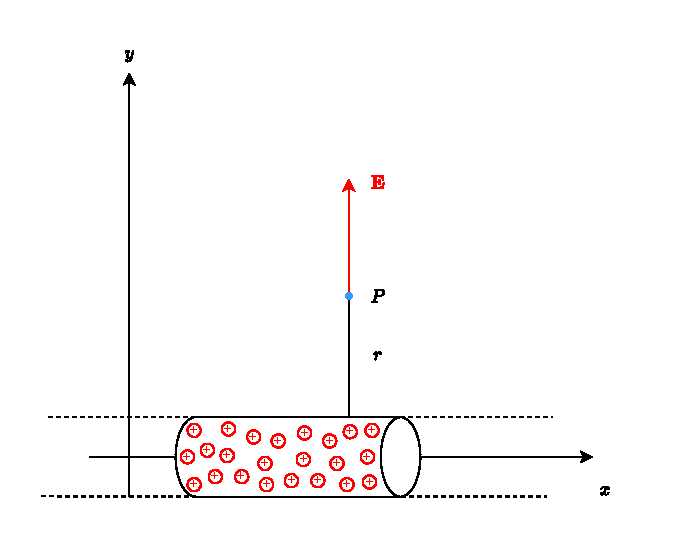
\includegraphics[width=0.6\linewidth]{res/svg/stationary_cable.drawio}
  \caption{Frame of reference $\irf{R}$}
\end{figure}
The point is at distance $r$, in the $y$ axis, from the cable, thus in $P$ there will be an electric field:
\begin{equation}
  \vec{E} = \dfrac{1}{2 \pi \epsz}\dfrac{\lambda}{r}\hat{u}_y
\end{equation}
Since the second IRF $\irf{R'}$ will in general be moving with respect to $\irf{R}$ with $\vec{v} \neq 0$, the point $P'$ will see charges in motion in the new frame of reference.
\begin{figure}[H]
  \centering
  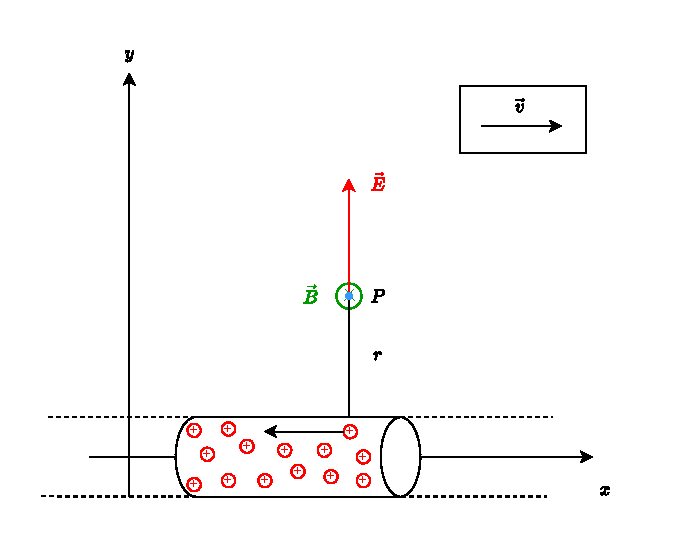
\includegraphics[width=0.6\linewidth]{res/svg/moving_cable.drawio}
  \caption{Frame of reference $\irf{R'}$}
\end{figure}
The linear charge density will be the same, since if one charge enters the ``field of view'' of $P$ another exits it, but, in this case $P'$ will also feel a magnetic field:
\begin{equation}
  \vec{B}' = \dfrac{\muz}{4 \pi}\dfrac{i}{r}\brackets{-\hat{u}_z}
\end{equation}
But, by actually measuring the fields in that point in space we do not see the effect of this seamingly ``newly-generated'' magnetic field. Also, if we check the conditions we got in \eqref{e:false_conditions} we can immediatly see that they are not satisfied.\\
Another example of the non-invariance of Electromagnetism are the potential equations in a vacuum at long distances:
\begin{equation}
  \begin{split}
    &\dalop \potE = 0\\[8pt]
    &\dalop \vec{A} = 0
  \end{split}
\end{equation}
The D'Alembert operator is not invariant under galilean transformations, in fact it would result that:
\begin{equation}
  \dalop = \dalop' -\dfrac{v^2}{c^2} \dfrac{\partial^2}{\partial x'^2} + \dfrac{v^2}{c^2} \pdv{}{x'}{t'}
\end{equation}
After those examples, if we want to preserve galilean transformations we must assume that there is only one IRF in which \maxwellref\;are true.\\
In order to try to solve this problem a new medium for electromagnetic waves propagation was hypotized and was called the \textbf{ether}, or, in latin \textit{etere luminifero}.\\
This new medium was defined more in a mathematical way rather than a physical one (and as we disucssed this is an issue). In fact, it was defined through the property it must satisfy.
Ether must:
\begin{itemize}
  \item be completely transparent to electromagnetic radiation
  \item have zero viscosity
  \item permeate all space
\end{itemize}
With the introduction of this new medium scientists supposed that \maxwellref\;may be true only in the IRF in which the motion of ether is stationary, so let's call:
\begin{quote}
  $\mathbfcal{R}_0$ is the only IRF (in which the ether is at rest) where the laws of Electromagnetism are true.
\end{quote}
This way of reasoning was not so new as we might think, since this would be the case for classical mechanical waves. If the medium of a wave goes faster/slower, then the wave itself goes faster/slower, we can only observe the ``pure'' wave motion if we are stationary with respect to the medium the wave is propagating inside.\\
Actually there was also another problem, since light travels at constant velocity $c$ in every direction we could find the only IRF in which this is true, but this is actually $\mathcal{R}_0$. This contradicts galilean relativity and would mean that electromagnetic measurements could tell us how any other IRF is moving with respect to $\mathcal{R}_0$. For this reason we can also define $\mathcal{R}_0$ as:
\begin{quote}
  $\mathbfcal{R}_0$ is the only optically isotropic reference frame
\end{quote}
\subsection{Michelson-Morley experiment}
There is a well-known experiment which wanted to prove the existence of ether, this experiment is known as the \textbf{Michelson-Morley experiment}. The two scientists created a setup consisting of an interferometre, a device in which a laser beam, generated by a source, splits into two other beams which travel along identical arms and then get reflected back into a screen.\\
The experimental setup is:
\begin{figure}[H]
  \centering
  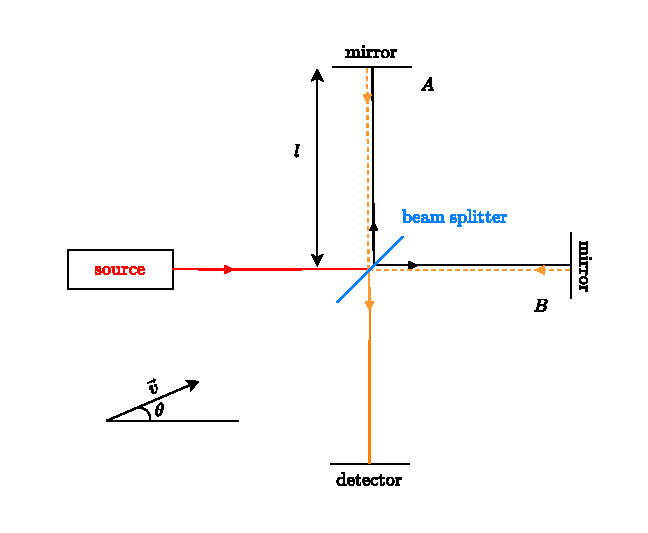
\includegraphics[width=0.6\linewidth]{res/svg/michelson_morley_experiment.drawio}
  \caption{Michelson-Morley interferometre}
\end{figure}
Since, at least once a year, Earth is moving with respect to the ether the two beams should take different paths with different length. This would mean that we should see an interference pattern appearing on the screen which will depend on the difference in time it takes to travel part A and part B. By doing the calculations we get:
\begin{equation}
  \Delta t = t_A - t_B = \dfrac{l}{c}\brackets{\dfrac{v}{c}}^2\cos(2\theta)
\end{equation}
So by moving the experimental setup, and thus changing the value of $\theta$, we might expect to see a difference in the measured time difference, but this was not the case. The measurements were conducted in different times of the year, but the results were pretty much against the hypotesis of ether. There were two possible explainations:
\begin{enumerate}
  \item Earth \underline{is} $\mathcal{R}_0$ and so light travels in any direction with speed $c$
  \item The ether has some sort of ``drag effect'' which would affect the experimental results
\end{enumerate}
The first explaination is just really unlikely, the second one contradicts the definition of ether itself, we would need an ether that both has zero viscosity, but also generates a drag effect. This basically makes zero sense.
\subsection{Stellar aberration}
Another contradiction of the ether model arises from the observation of a phenomenon called \textbf{stellar aberration}. Let's imagine that we want to capture the light emitted by a far away star. In order to do this we must put our telescope at an angle $\alpha$ since Earth is moving with respect to ether.
\begin{figure}[H]
  \centering
  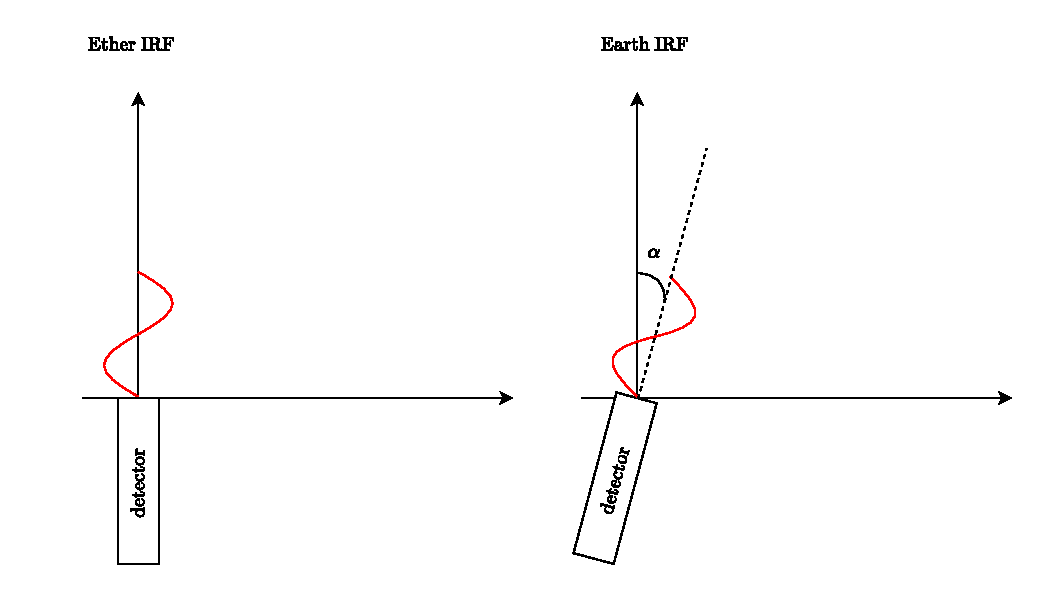
\includegraphics[width=0.6\linewidth]{res/svg/stellar_aberration.drawio}
  \caption{Stellar aberration}
\end{figure}
In particular, the angle must be the angle for which this condition is true:
\begin{equation}
  \tan \alpha = \dfrac{v}{c}
\end{equation}
Where $v$ is the velocity of Earth with respect to ether. According to the data collected by measurements $v \approx 3100 \unit{\meter / \second}$. This means that Earth should be moving with respect ot ether and this already contradicts the hypotesis that requires the IRF to be the same as the ether one. And so the explaination which considers the existence of ether for the Michelson-Morley experiment is not compatible with experimental data, therefore it must be rejected.
\subsection{Emission theory}
After the previous theories were rejected a new model was created. This is the \textbf{emission theory} model, which is based on some key concepts:
\begin{itemize}
  \item There is no ether
  \item There is no optically isotropic IRF
  \item Every source emits electromagnetic waves isotropically in their reference frame, which means that every IRF is isotropical for its radiation
\end{itemize}
This explains both the phenomenon of stellar aberration since the IRF of Earth is not the same as the source of the light, and it also explains Michelson-Morley experiment. Unfortunately this is not the case. To prove this we will now introduce an experimental observation that contradicts this theory.
\subsection{Binary stars}
Let's consider a system of two stars orbiting around each other. This system was described in 1913 by  Willem de Sitter.
\begin{figure}[H]
  \centering
  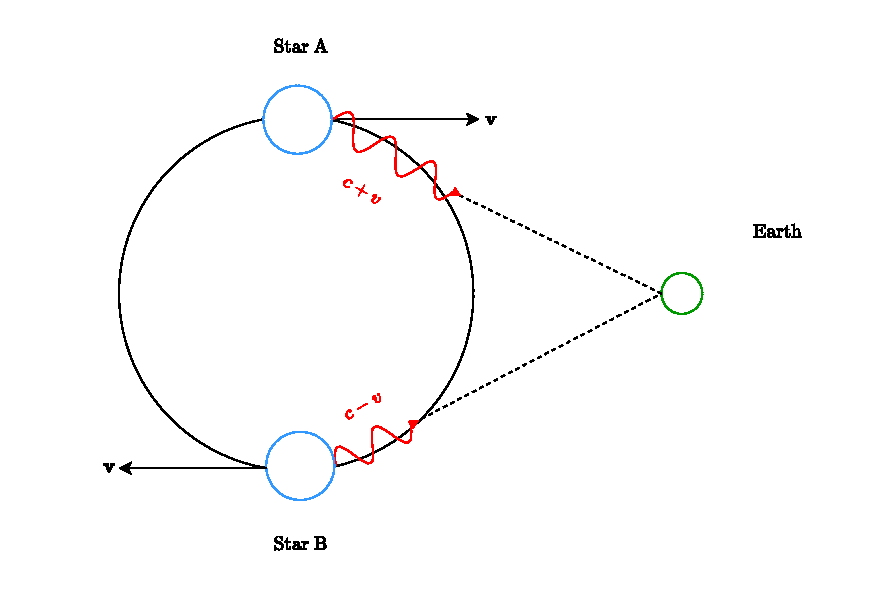
\includegraphics[width=0.6\linewidth]{res/svg/binary_stars.drawio}
  \caption{Binary stars system}
\end{figure}
If we apply the emission theory model we should expect to see that the intensity of light reaching us has some sort of periodic non-constant pattern, instead, experimental observation lead to seamingly unexplainable data. The intensity of the radiation was constant for most of the time and a minimum was periodically registered. The minimum of intensity corresponds with an eclipse event or, in other terms, when one of the stars covered the other and blocked its light.\\
One last attempt to save the ether hypotesis was done by introducing a correcting factor:
\begin{equation}
  \gamma = \dfrac{1}{\sqrt{1-\dfrac{v^2}{c^2}}}
\end{equation}
This factor was present in a new given hypotesis:
\begin{itemize}
  \item Lengths contract with a factor of $\gamma$ if the body is in motion with respect to Ether
  \item Clocks slow down with a factor of $\gamma$ if the body is in motion with respect to Ether
\end{itemize}
This factor was called \textbf{Lorentz factor} in the name of Hendrick Lorentz. The hypotesis of length contraction and time dilation was, at that time, just an \textit{ad hoc} hypotesis and was later proved to be insufficient to explain a Michelson-Morley type of experiment with different arms length. But as we might notice this already starts to look like something very similar to Einstein's hypotesis for Special Relativity, in fact the Lorentz factor was later used to develop \textbf{Lorentz transformations}, which are the starting point of Special Relativity.

\chapter{Fundamentals of Special Relativity}
\section{Principles of Special Relativity}
From our previous discussion we concluded that the only possible explaination would imply that Earth is the only optically isotropic IRF. But we know that Earth is orbiting the Sun and so in general it is not an IRF. We could say that for a short period of time Earth is actually an IRF since the velocity of the rotation around the Sun is approximately constant in a small time frame. This would mean that Earth is a sort of ``collection'' of IRFs that are all optically isotropic. But assuming that only the IRFs associated with the Earth's rotation are optically isotropic would imply an overly complicated and not really probable answer. By applying the famous philosophical principle of the ``Occam's razor'' we prefer the simpler explaination that all IRFs are optically isotropic.
From this Einstein states his two principles:
\begin{theorem}{First principle of relativity}
  \begin{itemize}
    \item All the IRFs are equivalent for the description of any physical phenomenon
    \item No experiment carried out in an IRF can help to distinguish the reference frame among the $\infty^3$ inertial reference frames
    \item ALl physical laws are the same in all IRFs
    \item No special or privileged IRF exists
  \end{itemize}
\end{theorem}
\begin{theorem}{Second principle of relativity}
  In an IRF, the speed of light does not depend on either the velocity of the source or on the direction of propagation.
\end{theorem}
Those principles are the foundations that will lead to all the results of Special Relativity. The first and probably most immediate example of this is the concept of simultaneity.
\subsection{Simultaneity}
In light of the two principles of relativity let's discuss the concept of simultaneity. Consistently to what we previously defined if we want to measure the time evolution of an event we must place a clock in every point of the Euclidean space, but we also need these clocks to be synchronized.\\
Our \textbf{first idea} might be to bring all the clocks at the origin, synchronize them and then put them in every point in space, but this reasoning is fundamentally flawed. We never asked in the first place for the clock to be invariant under translation in space.\\
A \textbf{second idea} would require to leave all the clocks in the space and somehow send a signal to synchronize the clocks. The clocks are synchronized if they show the same time simultaneously.\\
To define what simultaneity is in our new theory we must use something that is invariant under a change of IRF. If we imagine sending a voice signal to synchronize the clocks we immediately encounter difficulties since the speed of sound may vary under certain conditions. Instead, we exploit the fact that light travels in any direction at constant speed $c$. We can thus define a concept of simultaneity:
\begin{definition}{Simultaneity}
  Two events that occur in different points A, B are simultaneous if any observer at the same distance sees the events occur at the same time indicated by his own clock.
\end{definition}
From this we can understand why we asked for a Euclidean space, since the concept of distance is tied to Euclidean geometry.\\
Let's imagine a point $P$ in a two-dimensional IRF:
\begin{figure}[H]
  \centering
  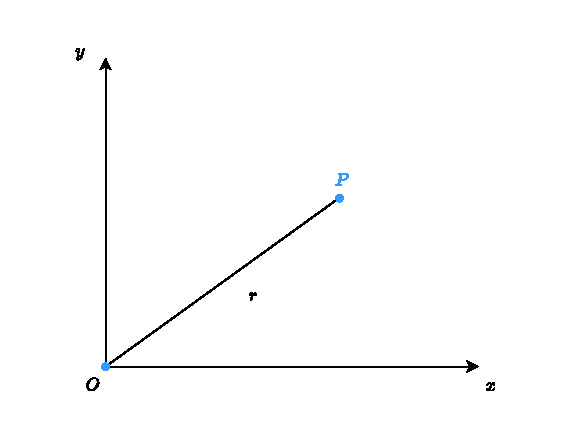
\includegraphics[width=0.6\linewidth]{res/svg/two_dim_IRF.drawio}
\end{figure}
The distance between the origin and $P$ will be:
\begin{equation}
  r = \overline{OP}
\end{equation}
If we send a signal through an electromagnetic wave, it will travel at the speed of light $c$ and reach the point $P$ in a time $t$ given by:
\begin{equation}
  t = \dfrac{r}{c}
\end{equation}
So to synchronize the two clocks, we can use the following procedure:
\begin{enumerate}
  \item Put the clock at distance $r$ already set to $\dfrac{r}{c}$
  \item Send a signal from the origin to the clock and start your clock
  \item When the signal reaches the clock, your clock will read $\dfrac{r}{c}$ and the other one will start from $\dfrac{r}{c}$ aswell
\end{enumerate}
From now on the clocks will be synchronized. This procedure puts us in the perspective that simultaneity is not an absolute concept.
\section{Lorentz transformations}
We need new transformations that work with the principles. We set two IRFs $\irf{R}$ and $\irf{R'}$ in the \textbf{standard configuration}, which means that the $x$ and $x'$ axes coincide and at time $t=0$ we have $O \equiv O'$. The two IRFs are moving with respect to each other with a velocity $v$ along the $x$ axis. Now an event occurs in $P'$, along the $x'$ axis which is at rest with respect to $\irf{R'}$, and we want to find the coordinates of the event in $\irf{R}$.
\begin{figure}[H]
  \centering
  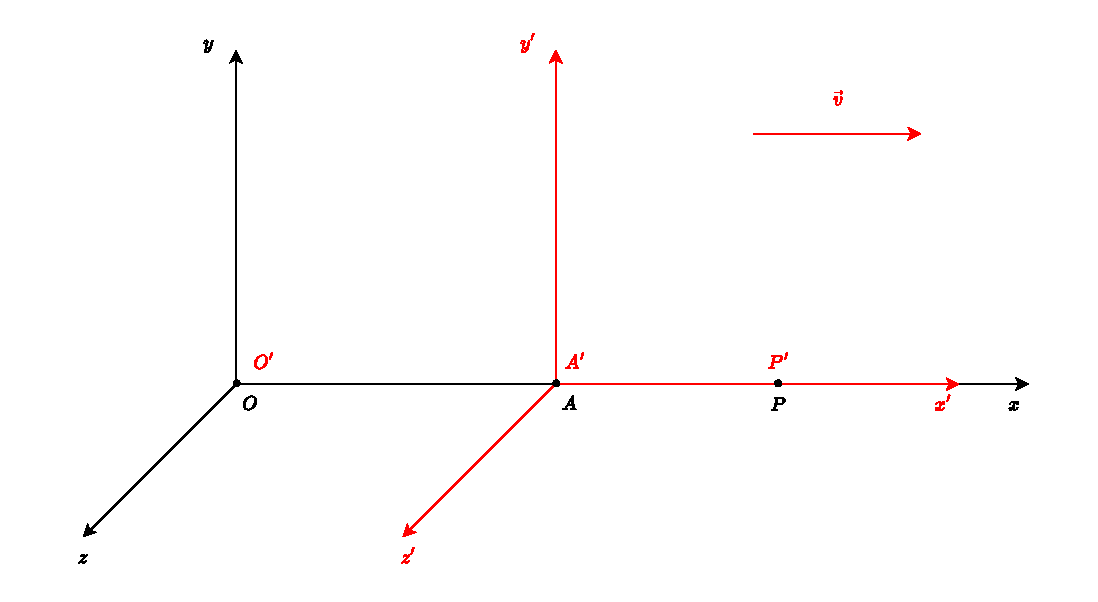
\includegraphics[width=0.6\linewidth]{res/svg/3d_IRF_lorentz.drawio}
  \caption{Moving IRFs}
\end{figure}
If we imagine putting a sort of sign $P$ when the event occurs we might think that it is sufficient to measure the distance $\overline{OP}$, but, in principle, our operational definition of length does not allow us to do that, since we only defined how to measure things at rest with respect to our IRF. Now imagine we mark the points $A'$ (origin of the moving IRF) and $P'$ (event) when the event occurs. The distance we measure will be some sort of proportionality relation depending on the speed of the IRF. We can write:
\begin{equation}
  \overline{A'P'} = \gamma (v)\overline{AP}
\end{equation}
And so:
\begin{equation}
  \overline{OP} = \overline{OA} + \overline{AP} = \overline{OA} + \dfrac{\overline{A'P'}}{\gamma (v)}
\end{equation}
We can also write:
\begin{equation}
  \overline{OA} = vt
\end{equation}
And so:
\begin{equation}
  \overline{OP} = vt + \dfrac{\overline{A'P'}}{\gamma (v)}
\end{equation}
This makes sense since $\gamma (v)$ will be equal to 1 when $v=0$ and so the distance in the second IRF will be equal to the distance we measure in the original one. We can also write:
\begin{equation}
  x = vt + \dfrac{x'}{\gamma(v)} \implies x' = \gamma(v)(x - vt)
\end{equation}
If $\gamma(v)$ were equal to 1, we would have the Galilean transformations. Doing the same reasoning in the other IRF we can find that:
\begin{equation}
 x = \gamma(-v)(x' + vt')
\end{equation}
But since there is no reason for gamma to change if we simply change the direction of the velocity $\gamma(-v) = \gamma(v)$, thus we have:
\begin{equation}
  \begin{split}
    &x = \gamma(v)(x' + vt') = \gamma(v)(\gamma(v)(x - vt) + vt') \\[8pt]
    &\dfrac{x}{\gamma(v)} = \gamma(v)x - \gamma(v)vt + vt' \\[8pt]
    &\underbrace{\dfrac{1}{v}\sqbr{\dfrac{1}{\gamma(v)}- \gamma(v)}}_{\nu(v)}x = t' - \gamma(v)t \\[8pt]
    &\nu(v)x + \gamma(v)t = t'
  \end{split}
\end{equation}
We found that:
\begin{equation} \label{e:lt_start}
  \begin{cases}
    x' = \gamma(v)(x - vt) \\[8pt]
    t' = \nu(v)x + \gamma(v)t \\[8pt]
    y'=y \\[8pt]
    z'=z
  \end{cases}
\end{equation}
We are done if we find the form of $\gamma(v)$. Let's use the fact that light travels at the same speed in both IRFs. Imagine sending a signal between two points at distance $\norm{\vec{r}}$. We have:
\begin{itemize}
  \item Event 1: S emits a signal at $t=t_1$. $E_1 = E_1(x_1, y_1, z_1, t_1)$
  \item Event 2: R receives the signal at $t=t_2$. $E_2 = E_2(x_2, y_2, z_2, t_2)$
\end{itemize}
The distances between the components of the positions of the events are:
\begin{equation}
  \begin{split}
    \Delta x = x_2 - x_1 \\[8pt]
    \Delta y = y_2 - y_1 \\[8pt]
    \Delta z = z_2 - z_1
  \end{split}
\end{equation}
And so the distance between $R$ and $S$ is:
\begin{equation}
  \norm{\Delta \vec{r}} = \sqrt{\Delta x^2 + \Delta y^2 + \Delta z^2}
\end{equation}
Since the signal travels at the speed of light, we have:
\begin{equation}
  \begin{split}
    &\Delta t = \dfrac{\norm{\vec{r}}}{c} = \dfrac{1}{c}\sqrt{\Delta x^2 + \Delta y^2 + \Delta z^2} \\[8pt]
    &\Delta t^2 = \dfrac{1}{c^2}\brackets{\Delta x^2 + \Delta y^2 + \Delta z^2} \\[8pt]
    &\underbrace{c^2\Delta t^2 - \Delta x^2 + \Delta y^2 + \Delta z^2}_{\Delta s^2} = 0\\[8pt]
  \end{split}
\end{equation}
In the second IRF we must have that:
\begin{equation}
  \dfrac{\norm{\Delta \vec{r}'}}{\Delta t'} = c
\end{equation}
And so, when the event occurs:
\begin{equation}
  \Delta s'^2 = \Delta s^2 = 0
\end{equation}
They are both zero since the two events are connected by a light signal. In general (except for light emission/ absorption events) the speed of the signal is not equal to $c$. We can write:
\begin{equation}
  \Delta s^2 = c^2\Delta t^2 - \Delta x^2 - \Delta y^2 - \Delta z^2 \neq 0
\end{equation}
Since the equations of transformation \eqref{e:lt_start} are linear and homogeneous, we know that the two $\Delta^2$s are proportional:
\begin{equation}
  \Delta s'^2 = \alpha \Delta s^2
\end{equation}
But since the events are arbitrary we can set only $\Delta z \neq 0$, but we also remember that $\Delta z = \Delta z'$ and so the only possible value of $\alpha$ is 1. Thus, we have:
\begin{equation}
  \Delta s'^2 = \Delta s^2
\end{equation}
And so $\Delta s$ is invariant under our new transformations. So going back to our original event we remember that the coordinates of $E_1$ are $E_1 = (0,0,0,0)$ and so:
\begin{equation}
  c^2 t^2 - x^2 - \cancel{ y^2} - \cancel{ z^2} = c^2 t'^2 - x'^2 - \cancel{ y'^2} -\cancel{ z'^2}
\end{equation}
Substituting the transformations \eqref{e:lt_start} we have:
\begin{equation}
  c^2 t^2 - x^2 = c^2 \sqbr{\nu(v)x + \gamma(v)t}^2 - \gamma(v)^2(x - vt)^2
\end{equation}
We can group the terms to find something like:
\begin{equation}
  Ax^2 + Bxt + Ct^2 = 0
\end{equation}
But in general this is only true if $A=B=C=0$. Setting $C$ to zero gives:
\begin{equation}
  C = c^2 - c^2\gamma(v)^2 + \gamma(v)^2v^2 = 0 \implies \gamma(v) = \dfrac{1}{\sqrt{1 - \dfrac{v^2}{c^2}}}
\end{equation}
This is exactly the Lorentz factor we introduced in the previous chapter.
\begin{figure}[H]
  \centering
  \includesvg[width=0.6\linewidth]{res/svg/lorentzfactor}
  \caption{Lorentz factor}
\end{figure}
From now on we call $\gamma(v)$ simply $\gamma$, and we can write the Lorentz transformations as:
\begin{equation} \label{e:lt}
  \begin{cases}
    x' = \gamma(x - vt) \\[8pt]
    y'=y \\[8pt]
    z'=z \\[8pt]
    t' = \gamma\brackets{t - \dfrac{v}{c^2}x} \\[8pt]
  \end{cases}
\end{equation}
These transformations are actually restricted to the motion along the $x$ axis, but we can easily extend them to the other axes by simply rotating the system as we will soon show. Here are some comments about these transformations:
\begin{itemize}
  \item $\gamma$ is always real and greater than 1 since $v<c$ always
  \item If $v \ll c$ we have $\gamma \approx 1$, and so we have the Galilean transformations
  \item If $v \approx c$ we have $\gamma \rightarrow \infty$
  \item If the two IRFs were not in the standard configuration, then the Lorentz transformations would still be linear but not homogeneous (we usually put ourselves in the standard configuration to avoid this problem)
  \item Since the Lorentz transformations are a linear system, we can write them in matrix form
\end{itemize}
Let's see what we can say about the last point. If we just take the vector:
\begin{equation}
  \begin{pNiceMatrix}
    x'\\[8pt]
    y'\\[8pt]
    z'\\[8pt]
    t'\\
  \end{pNiceMatrix}
\end{equation}
Then we have that the linear system \eqref{e:lt} is equivalent to:
\begin{equation}
  \begin{pNiceMatrix}
    x' \\[8pt]
    y' \\[8pt]
    z' \\[8pt]
    t' \\
  \end{pNiceMatrix}
  =
  \begin{pNiceMatrix}[columns-width=auto]
    \gamma & 0 & 0 & -\gamma v \\[8pt]
    0 & 1 & 0 & 0 \\[8pt]
    0 & 0 & 1 & 0 \\[8pt]
    -\gamma \dfrac{v}{c^2} & 0 & 0 & \gamma \\
  \end{pNiceMatrix}
  \begin{pNiceMatrix}
    x \\[8pt]
    y \\[8pt]
    z \\[8pt]
    t \\
  \end{pNiceMatrix}
\end{equation}
But this is rather ugly. In order to make this more elegant we do not use time, but $ct$ so that we have all lengths inside the vector. We then define the vector $x^{\mu}$:
\begin{equation}
  x^0 = ct, \quad x^1 = x, \quad x^2 = y, \quad x^3 = z
\end{equation}
We also define:
\begin{equation}
  \beta \defineeq \dfrac{v}{c}
\end{equation}
And so Lorentz transformations become:
\begin{equation}
  \begin{pNiceMatrix}
    x'^0 \\[8pt]
    x'^1 \\[8pt]
    x'^2 \\[8pt]
    x'^3 \\
  \end{pNiceMatrix}
  =
  \begin{pNiceMatrix}[columns-width=auto]
    \gamma & -\gamma \beta & 0 & 0 \\[8pt]
    -\gamma \beta & \gamma & 0 & 0 \\[8pt]
    0 & 0 & 1 & 0 \\[8pt]
    0 & 0 & 0 & 1 \\
  \end{pNiceMatrix}
  \begin{pNiceMatrix}
    x^0 \\[8pt]
    x^1 \\[8pt]
    x^2 \\[8pt]
    x^3 \\
  \end{pNiceMatrix}
\end{equation}
We define this matrix as the \textbf{Lorentz matrix} $\lm$:
\begin{equation}
  \lm \defineeq
  \begin{pNiceMatrix}[columns-width=auto]
    \gamma & -\gamma \beta & 0 & 0 \\[8pt]
    -\gamma \beta & \gamma & 0 & 0 \\[8pt]
    0 & 0 & 1 & 0 \\[8pt]
    0 & 0 & 0 & 1 \\
  \end{pNiceMatrix}
\end{equation}
\subsection{Composition of boosts}
If we have three IRFs $\irf{R}$, $\irf{R'}$ and $\irf{R''}$ such that $\irf{R'}$ moves with speed $v$ with respect to $\irf{R}$ and $\irf{R''}$ moves with speed $v'$ with respect to $\irf{R'}$. The two speeds are parallel, and we want to find at what speed $\irf{R''}$ moves with speed $v''$ with respect to $\irf{R}$. Obviously this will not just be:
\begin{equation}
  v'' \neq v' + v
\end{equation}
But, by applying the Lorentz transformations two times we get:
\begin{equation}
  v'' = \dfrac{v + v'}{1 + \dfrac{vv'}{c^2}}
\end{equation}
And so those notations are equivalent:
\begin{equation}
  \begin{split}
    &\irf{R} \xrightarrow{\lm(v)} \irf{R'} \xrightarrow{\lm(v')} \irf{R''}\\[8pt]
    &\irf{R} \overset{\lm(v'')}{\xrightarrow{\makebox[2.25cm]{}}} \irf{R''}
  \end{split}
\end{equation}
If we had a boost that isn't parallel to an axis we can just rotate the axes and so the transformation will become:
\begin{equation}
  \irf{R} \xrightarrow{R\lm} \irf{R'}
\end{equation}
The rotation + transformation notation used above is called \textbf{Thomas notation}. Clearly, the matrix $R$ represents the rotation matrix and the matrix $\lm$ still represents the Lorentz transformation. The most general homogeneous Lorentz transformation is then:
\begin{equation}
  R\lm_0
\end{equation}
\subsection{Inverse Lorentz transformations}
Now we can ask ourselves what the inverse of a Lorentz transformation is. We have two ways to determine this. The first is just to write down the equations, invert them and write the inverse matrix $\invlm$:
\begin{equation}
  \begin{cases}
    x' = \gamma(x - vt)\\[8pt]
    y'=y \\[8pt]
    z'=z \\[8pt]
    t' = \gamma\brackets{t - \dfrac{v}{c^2}x} \\[8pt]
  \end{cases}
  \xrightarrow{\text{invert}} \quad
  \begin{cases}
    x = \gamma(x' + vt') \\[8pt]
    y = y' \\[8pt]
    z = z' \\[8pt]
    t = \gamma\brackets{t' + \dfrac{v}{c^2}x'} \\[8pt]
  \end{cases}
\end{equation}
This is a bit long but not difficult.\\
\STOP Otherwise, we can just observe that the matrix $\lm$ can be easily inverted since the $2 \by 2$ block on the bottom right is just the identity matrix. The other block which contains $\gamma$ and $\beta$ can be inverted using the $2 \by 2$ matrix inversion rule. First define the submatrix:
\begin{equation}
  \lm_{2 \by 2} = \begin{pNiceMatrix}[columns-width=auto]
    \gamma & -\gamma \beta \\[8pt]
    -\gamma \beta & \gamma \\[8pt]
  \end{pNiceMatrix}
\end{equation}
Then find the inverse:
\begin{equation}
  \invlm_{2 \by 2} = \dfrac{1}{\det(\lm_{2x2})}\begin{pNiceMatrix}[columns-width=auto]
    \gamma & \gamma \beta \\[8pt]
    \gamma \beta & \gamma \\[8pt]
  \end{pNiceMatrix}
\end{equation}
But the determinant of the submatrix is just:
\begin{equation}
  \det(\lm_{2x2}) = \gamma^2 - \beta^2\gamma^2 = \gamma^2 \bbrackets{\underbrace{1 - \dfrac{v^2}{c^2}}_{1/\gamma^2}} = \cancel{ \gamma^2} \dfrac{1}{\cancel{\gamma^2}} = 1
\end{equation}
And so the inverse Lorentz matrix is:
\begin{equation}
  \invlm =
  \begin{pNiceMatrix}[columns-width=auto]
    \gamma & \gamma \beta & 0 & 0 \\[8pt]
    \gamma \beta & \gamma & 0 & 0 \\[8pt]
    0 & 0 & 1 & 0 \\[8pt]
    0 & 0 & 0 & 1 \\
  \end{pNiceMatrix}
\end{equation}
Which is equivalent to what we got by inverting the system.\\ (End of optional material)
\subsection{Vector form of Lorentz transformations}
For two IRFs in standard configuration we have that the unit vectors are the same:
\begin{equation}
  \begin{split}
    \hat{u}_{x} = \hat{u}_{x'}\\[8pt]
    \hat{u}_{y} = \hat{u}_{y'}\\[8pt]
    \hat{u}_{z} = \hat{u}_{z'}
  \end{split}
\end{equation}
We could represent Galilean transformations as a vector equation:
\begin{equation} \label{e:vector_galilean}
  \vec{r}' = \vec{r} - \vec{v}t
\end{equation}
Where the velocity is:
\begin{equation}
  \vec{v} =
  \begin{pNiceMatrix}
    v \\[8pt] 0 \\[8pt] 0
  \end{pNiceMatrix}
\end{equation}
What about Lorentz transformations? If we eplicitly write the equations we have:
\begin{equation}
  \vec{r}' = \gamma(x-vt)\hat{u}_{x} + y\hat{u}_{y} + z\hat{u}_{z} = \gamma x \hat{u}_{x} - vt\hat{u}_{x} + y\hat{u}_{y} + z\hat{u}_{z}
\end{equation}
If we add and subtract the $x$ component of the position vector we can write Lorentz transformations similarly to \eqref{e:vector_galilean}:
\begin{equation}
  \begin{split}
    \vec{r}' &= \gamma x \hat{u}_{x} - vt\hat{u}_{x} + y\hat{u}_{y} + z\hat{u}_{z} + x \hat{u}_{x} - x \hat{u}_{x}\\[8pt]
    \begin{pNiceMatrix}
      x' \\[8pt] y' \\[8pt] z'
    \end{pNiceMatrix}
    &= \begin{pNiceMatrix}
      x \\[8pt] y \\[8pt] z
    \end{pNiceMatrix}
    + \begin{pNiceMatrix}
      \brackets{\gamma -1}x + \gamma vt \\[8pt] 0 \\[8pt] 0
    \end{pNiceMatrix}
  \end{split}
\end{equation}
But this is not a really nice form. We can rewrite the unit vector and the $x$ component of $\vec{r}$ as:
\begin{equation}
  \begin{split}
    &\hat{u}_{x} = \dfrac{\vec{v}}{v} \\[8pt]
    &x = \vec{r} \cdot \hat{u}_{x} = \dfrac{\vec{r} \cdot \vec{v}}{v}
  \end{split}
\end{equation}
And so we have:
\begin{equation}
  \begin{split}
    \brackets{\gamma -1}x\hat{u}_{x} + \gamma vt\hat{u}_{x} &= \brackets{\gamma -1}\dfrac{\vec{r} \cdot \vec{v}}{v} \dfrac{\vec{v}}{v} + \gamma \cancel{v}t \dfrac{\vec{v}}{\cancel{v}} = \\[8pt]
    & = \vec{v} \sqbr{\brackets{\gamma -1}\dfrac{\vec{r} \cdot \vec{v}}{v^2} + \gamma t}
  \end{split}
\end{equation}
And so we can write Lorentz transformations as:
\begin{equation}
  \begin{cases}
    \vec{r}' = \vec{r} + \vec{v} \sqbr{\brackets{\gamma - 1} \dfrac{\vec{r} \cdot \vec{v}}{v^2} + \gamma t} \\[8pt]
    t' = \gamma \brackets{t - \dfrac{\vec{r} \cdot \vec{v}}{c^2}}
  \end{cases}
\end{equation}
The advantage of this form is that those equations are true for any boost in any direction.
\subsection{Time order}
These new transformations implicitly imply that there could be some ``weird'' stuff happening to the order of events. Since time and thus simultaneity depend on position and velocity we can ask ourselves if it is possible to find a couple of IRFs in motion with respect to each other such that an event $E_A(x_A,y_A,z_A,t_A)$ happens before a second event $E_B(x_B,y_B,z_B,t_B)$ in one IRF, but $E_B$ happens before $E_A$ in the other.\\
Let's start from two events only separated along the $x$ component. Defining the time interval $\Delta t = t_B - t_A$ we want that:
\begin{equation}
  \begin{split}
    &\Delta t > 0 \quad \text{in} \;\irf{R} \\[8pt]
    &\Delta t' < 0 \quad \text{in} \;\irf{R}'
  \end{split}
\end{equation}
We can just apply Lorentz transformations in the second equation and see what we find. Since they are linear we can substite $\Delta x$ instead of $x$ and $\Delta t$ instead of $t$, but in principle we should substite every single term and then group. We have:
\begin{equation}
  \Delta t' = \gamma \brackets{\Delta t - \dfrac{v}{c^2}\Delta x} < 0 \implies \Delta x > \dfrac{c^2}{v}\Delta t
\end{equation}
For any $v$ we know that $\dfrac{c}{v} > 1$, and so we can find that at least:
\begin{equation}
  \Delta x > c\Delta t
\end{equation}
But $\Delta x = c\Delta t$ is the distance travelled by light in a time interval $\Delta t$, so this means that in order to find a couple of IRFs where the time order of the events is swapped, we must make sure that the events are distant enough to satisfy:
\begin{equation}
  \Delta x > c\Delta t
\end{equation}
It is easy to generalize this condition:
\begin{equation}
  \Delta \norm{\vec{r}} > c\Delta t
\end{equation}
Where $\vec{r}$ is the distance vector between the points where the events take place.\\
This result also means that special relativity \textbf{preserves causality}. If an event is caused by another one there is no way for the signal that connects the two events to travel faster than light, and so we cannot see the time order reversed.
\subsection{Length contraction}
Let's go back to the starting configuration we used to derive Lorentz transformations. We found out that:
\begin{equation}
  \overline{AP} = \dfrac{\overline{A'P'}}{\gamma}
\end{equation}
Let's give a new definition:
\begin{definition}{Proper length}
  The proper length $L_0$ is the length measured in the IRF where the object is stationary.
\end{definition}
And so in our case $\overline{A'P'}$ is the proper length. We can see proper length as the only length that can be directly measured using our definition. We notice that, since $\gamma >1$:
\begin{equation}
  \overline{AP} < \overline{A'P'}
\end{equation}
Thus, proper length is the biggest length measured in any IRF. This result is widely known as \textbf{length contraction}.
\subsection{Time dilation}
We have a similar result for time. Let's imagine an IRF where two events happen in the same point but at different times. In any other IRF in motion with respect to the first one we have:
\begin{equation}
  \Delta t' = \gamma\brackets{\Delta t - \dfrac{v}{c^2}\cancel{\Delta x}} = \gamma \Delta t
\end{equation}
Since $\gamma > 1$ we have that:
\begin{equation}
  \Delta t' > \Delta t
\end{equation}
In this case the time separation between the two events is bigger for the moving observer. This effect is in fact called \textbf{time dilation}. Similarly to what we did with length we can give a new definition:
\begin{definition}{Proper time}
  The proper time $T_0$ is the time interval of the IRF where I measure it with only one clock.
\end{definition}
\subsection{Muons}
To showcase a real example, where the effect of time dilation and length contraction play a crucial role in explaining the phenomenon, we will now talk about \textbf{muons} $\mu$. Muons are a type of elementary particles with these properties:
\begin{itemize}
  \item Charge: $q_{\mu} = -e$
  \item Mass: $m_{\mu} \ll m_{e}$
  \item Proper time decay: $T_0 = \qty{2.2}{\micro\second}$
\end{itemize}
\begin{figure}[H]
  \centering
  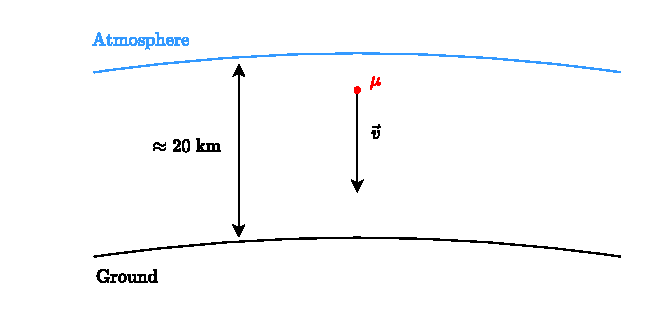
\includegraphics[width=0.8\linewidth]{res/svg/muons_bad.drawio}
  \caption{Muons travelling in Earth's atmosphere}
\end{figure}
Muons are generated by cosmic rays when hitting Earth's atmosphere and, after being generated, they travel at $v \approx 99.89\%\;c$ with a Lorentz factor of $\gamma \approx 30$. Muons were experimentally detected at Earth's surface, but if we apply a classical reasoning, in order to reach the surface of Earth, muons should travel a distance $\Delta x$ in a time less or equal to $T_0$, but this is not the case since $\Delta x \approx \qty{20}{\kilo\meter}$ and so:
\begin{equation}
  \dfrac{\Delta x}{v} \approx \qty{66.7}{\micro\second}
\end{equation}
Instead, applying Einstein's Special Relativity we know that the muon's time is dilated and so:
\begin{equation}
  T_0' = \gamma T_0 = \qty{66}{\micro\second}
\end{equation}
And so this result is compatible with the experimental observations. We can also think that the muon sees Earth travelling with speed $v$ in his direction and so the distance $\Delta x$ will be contracted:
\begin{equation}
  \Delta x' = \dfrac{\Delta x}{\gamma} \approx \qty{666.7}{\meter}
\end{equation}
Thus, the time it would take for the muon to travel this path is:
\begin{equation}
  \dfrac{\Delta x'}{v} \approx \qty{2.23}{\micro\second}
\end{equation}
Again this is coherent with the experimental evidence.
\subsection{Lorentz transformations of the velocities}
In a simple Galilean transformation the velocities are obtained by deriving with respect to time each component of the position:
\begin{equation}
  \begin{cases}
    x' = x - vt \\[8pt]
    y' = y \\[8pt]
    z' = z
  \end{cases} \xrightarrow{\frac{\diff{}}{\diff{t}}}
  \begin{cases}
    u'_x = u_x - v \\[8pt]
    u'_y = u_y \\[8pt]
    u'_z = u_z
  \end{cases}
\end{equation}
But in Lorentz transformation we need to evaluate the derivative of the new coordinates with respect to the new time. Writing Lorentz transformations for an infinitesimal displacement gives:
\begin{equation}
  \begin{cases}
    \diff{x'} = \gamma \brackets{\diff{x} - v \diff{t}} \\[8pt]
    \diff{y'} = \diff{y} \\[8pt]
    \diff{z'} = \diff{z} \\[8pt]
    \diff{t'} = \gamma \brackets{\diff{t} - \dfrac{v}{c^2} \diff{x}}
  \end{cases}
\end{equation}
And so $u'_x$ becomes:
\begin{equation}
  \begin{split}
    u'_x = \dv{x'}{t'} &= \dfrac{\cancel{\gamma} \brackets{\diff{x} - v \diff{t}}}{\cancel{\gamma} \brackets{\diff{t} - \dfrac{v}{c^2} \diff{x}}} =\\[8pt]
    &= \cancel{\dv{t}{t}}\dfrac{\brackets{\dv{x}{t} - v}}{\brackets{1 - \dfrac{v}{c^2} \dv{x}{t}}} = \dfrac{u_x - v}{1 - \dfrac{v u_x}{c^2} }
  \end{split}
\end{equation}
Instead for $u_y$ we have:
\begin{equation}
  \begin{split}
    u'_y = \dv{y'}{t'} &= \dfrac{\diff{y}}{\gamma \brackets{\diff{t} - \dfrac{v}{c^2} \diff{x}}} =\\[8pt]
  &= \dv{y}{t}\dfrac{\sqrt{1-\dfrac{v^2}{c^2}}}{\brackets{1 - \dfrac{v}{c^2} \dv{x}{t}}} = \dfrac{u_y\sqrt{1-\dfrac{v^2}{c^2}}}{1 - \dfrac{v u_x}{c^2}}
  \end{split}
\end{equation}
The same derivation leads to $u'_z$:
\begin{equation}
  u'_z = \dfrac{u_z\sqrt{1-\dfrac{v^2}{c^2}}}{1 - \dfrac{v u_x}{c^2}}
\end{equation}
And so the Lorentz transformation of the velocities for a boost along the x-axis are:
\begin{equation}
  \begin{cases}
    u'_x = \dfrac{u_x - v}{1 - \dfrac{v u_x}{c^2}} \\[18pt]
    u'_y = \dfrac{u_y\sqrt{1-\dfrac{v^2}{c^2}}}{1 - \dfrac{v u_x}{c^2}} \\[18pt]
    u'_z = \dfrac{u_z\sqrt{1-\dfrac{v^2}{c^2}}}{1 - \dfrac{v u_x}{c^2}}
  \end{cases}
\end{equation}
If we want to invert the equations and get $u_x, u_y, u_z$ as functions of the new coordinates we simply substitute $v \rightarrow -v$ since the only thing that changes is the direction of $v$:
\begin{equation}
  \begin{cases}
    u_x = \dfrac{u'_x + v}{1 + \dfrac{v u'_x}{c^2}} \\[18pt]
    u_y = \dfrac{u'_y\sqrt{1-\dfrac{v^2}{c^2}}}{1 + \dfrac{v u'_x}{c^2}} \\[18pt]
    u_z = \dfrac{u'_z\sqrt{1-\dfrac{v^2}{c^2}}}{1 + \dfrac{v u'_x}{c^2}}
  \end{cases}
\end{equation}
Now we can see how the magnitude of $u$ changes with a Lorentz transformation. After some calculations it is possible to arrive to:
\begin{equation}
  c^2 - u^2 = \dfrac{c^2\brackets{c^2 - u'^{^2}}\brackets{c^2 - v^2}}{\brackets{c^2 + u'_x v}}
\end{equation}
If we write $u_x$ as:
\begin{equation}
  u_x' = \vec{u}' \cdot \hat{u}_x = \vec{u}' \cdot \dfrac{\vec{v}}{v}
\end{equation}
We have:
\begin{equation}
  c^2 - u^2 = \dfrac{c^2\brackets{c^2 - u^{'^2}}\brackets{c^2 - v^2}}{\brackets{c^2 + \vec{u}'\cdot\vec{v}}}
\end{equation}
This also leads to the result that:
\begin{equation}
  u' < c \iff u < c
\end{equation}
The meaning of this is that, even if an object is moving at speed close to $c$ and another object is thrown from the moving one, the velocity of the thrown item can never be equal or greater to $c$.\\
It is possible to arrive to a vector form of the transformation of velocities. Similarly to what we did to the components we have:
\begin{equation}
  \vec{u}' = \dv{\vec{r}'}{t'}
\end{equation}
After some calculations we arrive to:
\begin{equation}
  \vec{u}' = \dfrac{\dfrac{\vec{u}}{\gamma(v)}+ \vec{v}\sqbr{\dfrac{\vec{u}\cdot\vec{v}}{v^2}\brackets{1-\dfrac{1}{\gamma(v)}}-1}}{1 - \dfrac{\vec{u}\cdot\vec{v}}{c^2}}
\end{equation}
Inverting this equation gives:
\begin{equation}
  \vec{u} = \dfrac{\dfrac{\vec{u}'}{\gamma(v)} - \vec{v}\sqbr{-\dfrac{\vec{u}'\cdot\vec{v}}{v^2}\brackets{1-\dfrac{1}{\gamma(v)}}-1}}{1 + \dfrac{\vec{u}'\cdot\vec{v}}{c^2}}
\end{equation}
Those two formulas are sometimes expressed as the result of a new operation called \textbf{relativistic addition}:
\begin{equation}
  \begin{split}
    \vec{u}' = \vec{v} \oplus \vec{u} \\[8pt]
    \vec{u} = \vec{v} \oplus \vec{u}'
  \end{split}
\end{equation}
Note that this operation is not linear and is not commutative:
\begin{equation}
  \vec{v} \oplus \vec{u} \neq \vec{u} \oplus \vec{v}
\end{equation}
But the magnitude of the results are the same:
\begin{equation}
  \norm{\vec{v} \oplus \vec{u}} = \norm{\vec{u} \oplus \vec{v}}
\end{equation}
Now let's analyse the case where $\vec{v} \perp \vec{u}'$ we have:
\begin{equation}
  \vec{u} = \dfrac{\dfrac{\vec{u}'}{\gamma(v)} - \vec{v}\sqbr{-\dfrac{\cancel{\vec{u}'\cdot\vec{v}}}{v^2}\brackets{1-\dfrac{1}{\gamma(v)}}-1}}{1 + \dfrac{\cancel{\vec{u}'\cdot\vec{v}}}{c^2}} = \dfrac{\vec{u}'}{\gamma (v)} + \vec{v}
\end{equation}
And so for a boost in this configuration:
\begin{figure}[H]
  \centering
  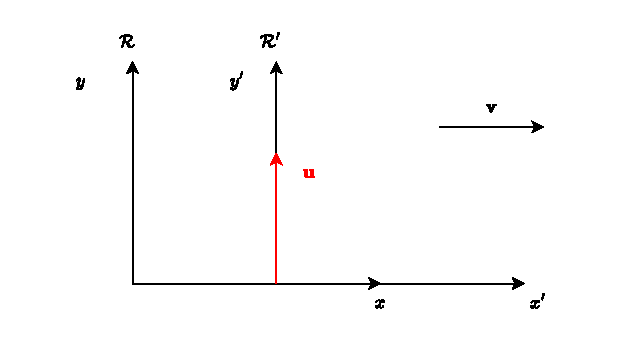
\includegraphics[width=0.6\linewidth]{res/svg/perpendicular_moving.drawio}
\end{figure}
We have that the relativistic addition is just scaled down of a factor $\gamma$ along the $\vec{u}$ vector:
\begin{figure}[H]
  \centering
  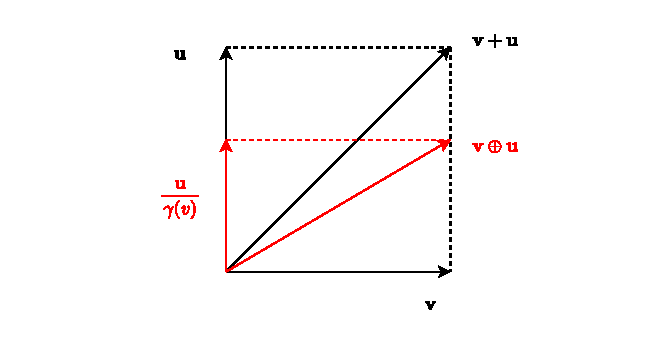
\includegraphics[width=0.8\linewidth]{res/svg/relativistic_addition.drawio}
\end{figure}
\subsection{Lorentz transformation of the $\gamma$ factor}
The Lorentz factor of a moving object changes with respect to the IRF. We have that:
\begin{equation}
  \dfrac{\gamma(u')}{\gamma(u)} = \gamma(v)\brackets{1-\dfrac{\vec{v}\cdot\vec{u}}{c^2}}
\end{equation}
Since this is in vector form it is valid for any boost.
\section{Examples (WIP)}
\section{Doppler effect}
Let us now describe a phenomenon arising from the properties of special relativity, this phenomenon is called \textbf{Relativistic Doppler effect}. First we need to discuss the classical derivation of the Doppler effect.
\begin{figure}[H]
  \centering
  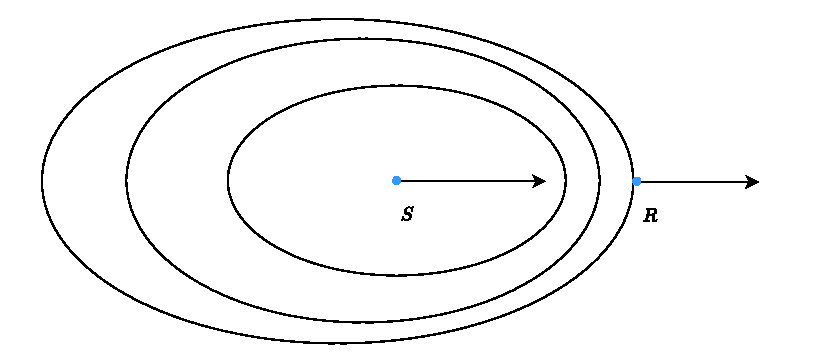
\includegraphics[width=1\linewidth]{res/svg/classical_doppler_diagram.drawio}
\end{figure}
The problem is described with these informations:
\begin{itemize}
  \item A source $S$ generates a signal at time $t=0$
  \item A receiver $R$ receives the signal
  \item The starting distance between the two is $l_0$
  \item Both the receiver and the source are moving in the same direction with, in general, different velocities
\end{itemize}
The fourth assumption is justified since if the source travels in another direction, the only significant component of the velocity that causes the Doppler effect is the component along the line from the source to the receiver.
Now let's start with the discussion.\\
The signal sent by the source reaches the receiver at time $\tau$, but what distance did the signal travel?\\
\begin{figure}[H]
  \centering
  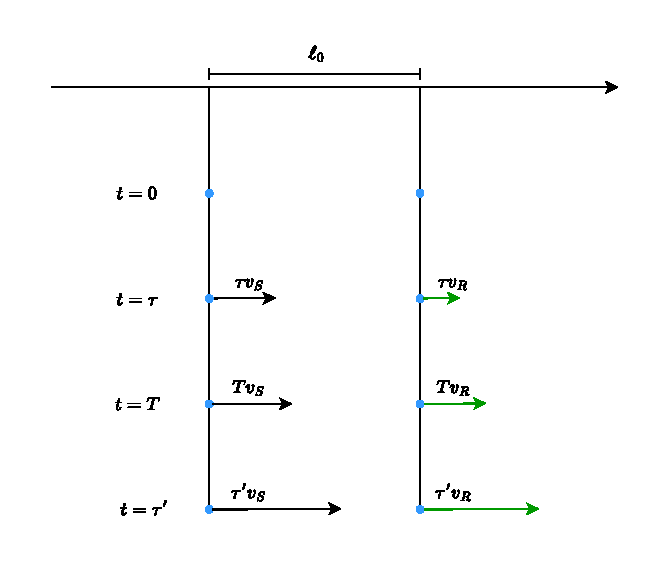
\includegraphics[width=0.8\linewidth]{res/svg/classical_doppler_distances.drawio}
\end{figure}
Since the receiver is moving we need to add the distance travelled by it in the time $\tau$, so:
\begin{equation}
  L_{true} = l_0 + v_{R}\tau
\end{equation}
And so the wave with velocity $v$ travelled $L_{true}$ space in $\tau$ time:
\begin{equation}
  v\tau = l_0 + v_{R}\tau \implies \tau = \dfrac{l_0}{v-v_{R}}
\end{equation}
Now, at time $T$ the source emits another signal, which arrives at the receiver at time $\tau'$, but then the length travelled in the time interval $\tau'-T$ is:
\begin{equation}
  L'_{true} = l_0 - v_{S}T + v_{R}\tau'
\end{equation}
And so:
\begin{equation}
  \begin{split}
    v(\tau'-T) &= l_0 - v_{S}T + v_{R}\tau' \\[8pt]
    \tau'(v-v_{R}) &= l_0 -v_{S}T + vT \\[8pt]
    \tau' &= \dfrac{l_0 +T(v-v_{S})}{v-v_{R}}
  \end{split}
\end{equation}
What is the period between the two signals? We define $T' = \tau' - \tau$ and so:
\begin{equation}
  T' = \dfrac{\cancel{l_0} +T(v-v_{S}) - \cancel{l_0}}{(v-v_{R})} = \dfrac{v-v_{S}}{v-v_{R}}T
\end{equation}
Since the frequency is just the inverse of the period:
\begin{equation}
  \boxed{\nu' = \dfrac{v-v_{R}}{v-v_{S}}\nu'}
\end{equation}
After this we can start to describe the relativistic version of this problem. The differences between the two situations are essentially three:
\begin{itemize}
  \item The signal does not propagate in a medium
  \item The relative velocity, in general, is not moving along the direction $S-R$, but is a generic $\vec{v}$
\end{itemize}
Let's choose two IRFs:
\begin{itemize}
  \item $\irf{R}$ is such that $R$ is stationary
  \item $\irf{R'}$ is such that $S$ is stationary
\end{itemize}
The first event is:
\begin{quotation}
  Event A: $S$ emits light in $O \equiv O'$ at time $t = t' = 0$
\end{quotation}
Now we state that phase is Lorentz invariant (this will be more clear later), thus both observers will agree on seeing when the EM fields are at a peak:
\begin{equation}
  k_{R}r-\omega_{R} t = k_{S}r' - \omega_{S} t'
\end{equation}
Let's group the angular frequencies, knowing that $\dfrac{k}{\omega} = \dfrac{2\pi}{\lambda}\dfrac{1}{2\pi\nu} = \dfrac{1}{c}$ we get:
\begin{equation}
  \omega_{R}\brackets{t-\dfrac{r}{c}} = \omega_{S}\brackets{t'-\dfrac{r'}{c}}
\end{equation}
Now let's picture the situation when the receiver registers the signal:
\begin{quotation}
  Event B: $R$ receives the signal
\end{quotation}
\begin{figure}[H]
  \centering
  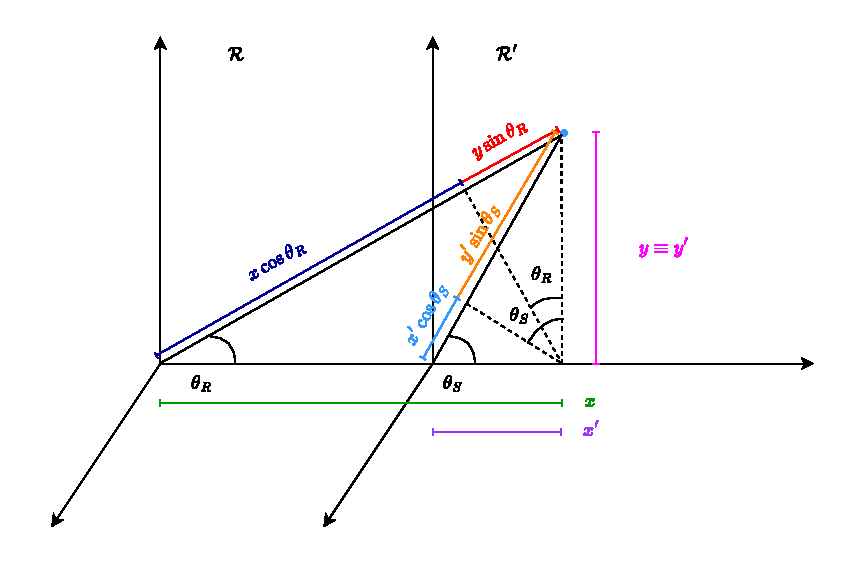
\includegraphics[width=0.8\linewidth]{res/svg/Doppler_geometry.drawio}
\end{figure}
So the modulus of $\vec{r}$ and $\vec{r}'$ are:
\begin{equation}
  \begin{split}
    &r = x\cos\theta_R + y\sin\theta_R \\[8pt]
    &r' = x'\cos\theta_S + y'\sin\theta_S
  \end{split}
\end{equation}
And so, since the two phases must be equal:
\begin{equation}
  \omega_{R}\sqbr{t-\dfrac{1}{c}\brackets{x\cos\theta_R + y\sin\theta_R}} = \omega_{S}\sqbr{t'-\dfrac{1}{c}\brackets{x'\cos\theta_S + y'\sin\theta_S}}
\end{equation}
Now we substite what we know from the Lorentz transformation of this system:
\begin{equation}
  \begin{cases}
    x' = \gamma(x - vt) \\[8pt]
    y' = y \\[8pt]
    t' = \gamma\brackets{t - \dfrac{v}{c^2}x}
  \end{cases}
\end{equation}
Thus the equation will be:
\begin{equation}
  \omega_{R}\sqbr{t-\dfrac{1}{c}\brackets{x\cos\theta_R + y\sin\theta_R}} = \omega_{S}\sqbr{\gamma\brackets{t - \dfrac{v}{c^2}x} - \dfrac{1}{c}\brackets{\gamma(x - vt)\cos\theta_S + y\sin\theta_S}}
\end{equation}
This must be true for all $x,y,t$ and so every coefficient must coincide.\\
For $t$ (1):
\begin{equation}
  \omega_R  = \omega_S \gamma\brackets{1 + \dfrac{v}{c}\cos \theta_S}
\end{equation}
For $x$ (2):
\begin{equation}
  \begin{split}
    \cancel{-}\dfrac{\omega_R}{\cancel{c}}\cos \theta_R &= \cancel{-}\omega_S \dfrac{\gamma}{\cancel{c}}\brackets{\dfrac{v}{c} + \cos \theta_S}\\[8pt]
    \cos \theta_R  &= \dfrac{\omega_S}{\omega_R} \gamma \brackets{\dfrac{v}{c} + \cos \theta_S} =\\[8pt]
    &\overset{(1)}{=} \dfrac{1}{\cancel{\gamma}\brackets{1 + \dfrac{v}{c}\cos \theta_S}} \cancel{\gamma} \brackets{\dfrac{v}{c} + \cos \theta_S} =\\[8pt]
    &= \dfrac{\dfrac{v}{c} + \cos \theta_S}{1 + \dfrac{v}{c}\cos \theta_S}
  \end{split}
\end{equation}
For $y$ (3):
\begin{equation}
  \begin{split}
    \cancel{-}\dfrac{\omega_R}{\cancel{c}}\sin \theta_R &= \cancel{-}\omega_S \dfrac{\gamma}\sin \theta_S\\[8pt]
    \sin \theta_R &= \dfrac{\omega_S}{\omega_R}\sin \theta_S = \\[8pt]
    &\overset{(1)}{=} \dfrac{1}{\gamma\brackets{1 + \dfrac{v}{c}\cos \theta_S}}\sin \theta_S = \\[8pt]
    &= \dfrac{\sqrt{1-\dfrac{v^2}{c^2}}}{1 + \dfrac{v}{c}\cos \theta_S}\sin \theta_S
  \end{split}
\end{equation}
And so, from (1) and (2) we can evaluate $\tan \theta_R$:
\begin{equation}
  \begin{split}
    \tan \theta_R = \dfrac{\sin \theta_R}{\cos \theta_R} &= \dfrac{\dfrac{\sqrt{1-\dfrac{v^2}{c^2}}}{1 + \dfrac{v}{c}\cos \theta_S}\sin \theta_S}{\dfrac{\dfrac{v}{c} + \cos \theta_S}{1 + \dfrac{v}{c}\cos \theta_S}} = \\[8pt]
    &= \dfrac{\sqrt{1-\dfrac{v^2}{c^2}}\sin \theta_S}{\cos \theta_S + \dfrac{v}{c}} = \\[8pt]
    &= \dfrac{c\sqrt{1-\dfrac{v^2}{c^2}}\sin \theta_S}{c\cos \theta_S + v}
  \end{split}
\end{equation}
Let's compare this to what we got for the transformation of the velocities:
\begin{equation}
  \tan \theta = \dfrac{u'\sin \theta'}{u'\cos \theta' + u}\dfrac{1}{\gamma}
\end{equation}
This is the same formula with:
\begin{equation}
  \begin{split}
    &u' = c \\[8pt]
    &\theta = \theta_R \\[8pt]
    &\theta' = \theta_S
  \end{split}
\end{equation}
If we write down both the relativistic and the classical Doppler effect we have:
\begin{equation}
  \begin{split}
    \omega_R  = \omega_S \gamma\brackets{1 + \dfrac{v}{c}\cos \theta_S} \\[8pt]
    \omega_R = \omega_S \dfrac{v - v_R}{v - v_S}
  \end{split}
\end{equation}
The two phenomenona cannot be really compared since the EM waves which generate the relativistic version of the Doppler effect do not require a medium to travel, but if we see that $-v \cos \theta_S$ is actually the tangential component of $v$ in the IRF $\irf{R}'$, thus it is similar to $v_R$ and we can write:
\begin{equation}
  \omega_R  = \omega_S \gamma\dfrac{c - v}{c}
\end{equation}
This relation is similar to the classical one with two exceptions:
\begin{enumerate}
  \item $v_S = 0$ in the relativistic case. The only quantity that matters is the relative velocity between the source and the receiver
  \item The Lorentz factor $\gamma$ is present
\end{enumerate}
This leads to a new situation which was not present in the classical case. If we consider a source in tangential motion there is no classical Doppler effect since the distance is kept constant, but in the relativistic case we have a transverse Doppler effect:
\begin{equation}
  \theta_S = \dfrac{\pi}{2} \implies \cos \theta_S = 0
\end{equation}
And so:
\begin{equation}
  \omega_R  = \omega_S \gamma \implies \omega_R  > \omega_S
\end{equation}
This effect is called \textbf{Blue shift} since the light that arrives at the receiver has a higher frequency, which results in a smaller wavelength and so, for example, a red beam of light will be shifted towards blue.\\
Similarly, if a source is moving away from the observer we have:
\begin{equation}
  \theta_S = \pi \implies \cos \theta_S = -1
\end{equation}
Which leads to:
\begin{equation}
  \begin{split}
    \omega_R  &= \omega_S \gamma\brackets{1 - \dfrac{v}{c}} = \\[8pt]
    &= \omega_S \dfrac{1 - \dfrac{v}{c}}{\sqrt{1 - \dfrac{v^2}{c^2}}} = \\[8pt]
    &= \omega_S \sqrt{\dfrac{\brackets{1 - \dfrac{v}{c}}^{\cancel{2}}}{\cancel{\brackets{1 - \dfrac{v}{c}}}\brackets{1 + \dfrac{v}{c}}}} = \\[8pt]
    &= \omega_S \sqrt{\dfrac{\brackets{1 - \dfrac{v}{c}}}{\brackets{1 + \dfrac{v}{c}}}}
  \end{split}
\end{equation}
This means that $\omega_R < \omega_S$, and so we have a higher wavelength. This phenomenon is called \textbf{Red shift}.
\begin{figure}[H]
    \begin{minipage}{0.5\textwidth}
     \centering
     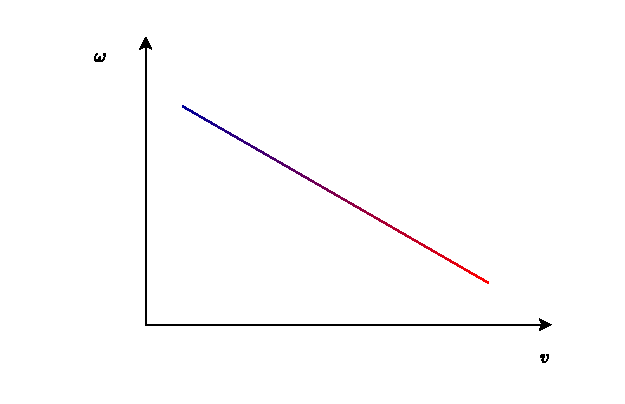
\includegraphics[width=1\linewidth]{res/svg/Doppler_redshift.drawio}
     \caption{Red shift}
   \end{minipage}\hfill
   \begin{minipage}{0.5\textwidth}
     \centering
     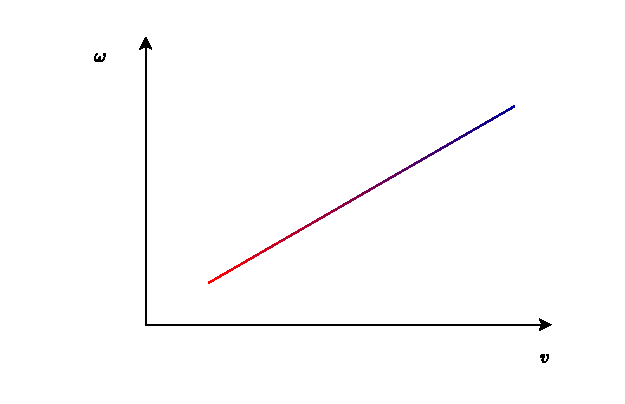
\includegraphics[width=1\linewidth]{res/svg/Doppler_blueshift.drawio}
     \caption{Blue shift}
   \end{minipage}
\end{figure}
\STOP We can check that the coefficients of $\omega_R = K\omega_S$ in the cases of rotations of $n\dfrac{\pi}{2}$ are related to the eigenvalues associated to the Lorentz matrix.\\
We know that $1$ will be an eigenvalue because of the 2x2 block on the bottom right of the Lorentz matrix, so we just need the eigenvalues of the $2 \by 2$ block on the top left:
\begin{equation}
  \lm_{2 \by 2} = \begin{pNiceMatrix}[columns-width=auto]
    \gamma & -\gamma \beta \\[8pt]
    -\gamma \beta & \gamma \\[8pt]
  \end{pNiceMatrix}
\end{equation}
We find $\lambda_1, \lambda_2$ by the usual method:
\begin{equation}
  p(\lambda) = \det(\lm_{2 \by 2} - \lambda \mathbb{I}) = \brackets{\gamma - \lambda}^2 - \gamma^2\beta^2 = \gamma^2 -2\gamma\lambda +\lambda^2 - \gamma^2\beta^2
\end{equation}
Finding the eigenvalues means:
\begin{equation}
  p(\lambda) = 0 \implies \lambda^2 -2\cancel{\gamma}\lambda + \gamma^{\cancel{2}}- \gamma^{\cancel{2}}\beta^2 = 0 \\[8pt]
\end{equation}
\begin{equation}
  \begin{split}
    &\dfrac{1}{\gamma}\lambda^2 -2\lambda +\gamma \brackets{1- \beta^2} = 0 \\[8pt]
    &\dfrac{1}{\gamma}\lambda^2 -2\lambda + \dfrac{1}{\sqrt{1-\beta^2}} \brackets{1- \beta^2} = 0 \\[8pt]
    &\dfrac{1}{\gamma}\lambda^2 -2\lambda + \sqrt{\dfrac{\brackets{1- \beta^2}^2}{1-\beta^2}}  = 0 \\[8pt]
    &\sqrt{1- \beta^2}\lambda^2 -2\lambda + \sqrt{1- \beta^2}  = 0 \\[8pt]
  \end{split}
\end{equation}
And so the roots are easily found by:
\begin{equation}
  \begin{split}
    \lambda_{1,2} &= \dfrac{2\pm\sqrt{4 - 4\brackets{1-\beta^2}}}{2} =\\[8pt]
    & = \dfrac{2\pm\sqrt{\cancel{4} - \cancel{4} +4\beta^2}}{2} =\\[8pt]
    & = \dfrac{2 \pm 2\beta}{2} = 1 \pm \beta
  \end{split}
\end{equation}
Thus the set of all the eigenvalue of $\lm$ is:
\begin{equation}
  \mathrm{spec}(\lm) = \{1, 1 \pm \beta\}
\end{equation}
Notice that for the various cases of rotations of $\dfrac{n\pi}{2}$ we have:
\begin{table}[H]
  \centering
  \begin{tabular}{lc}
    $\omega_R = \gamma \brackets{1-\beta} \omega_S$ & (for $n$ = 1) \\[8pt]
    $\omega_R = \gamma \omega_S$ & (for $n$ = 2) \\[8pt]
    $\omega_R = \gamma \brackets{1+\beta} \omega_S$ & (for $n$ = 3) \\[8pt]
    $\omega_R = \gamma \omega_S$ & (for $n$ = 4) \\[8pt]
  \end{tabular}
\end{table}
(End of optional material)
\begin{exercise}{TO DO}

\end{exercise}

\chapter{Tensor formalism}
\section{Introduction to tensors}
As we anticipated earlier in our discussion any couple of IRFs $\irf{R}, \irf{R}'$ can be obtained by using two transformations:
\begin{enumerate}
  \item Rotation, in order to make the axis be aligned \label{rotation_transformation}
  \item Translation, in order to make the origins coincide at some point in time \label{shift_transformation}
\end{enumerate}
If we can apply both \eqref{rotation_transformation} and \eqref{shift_transformation} we are in the so called \textbf{Poincarè group}, instead, if we only apply \eqref{rotation_transformation} we are in the \textbf{Lorentz group}, which, of course is a subgroup of the Poincarè group.\\
We also said that any event in Special Relativity has 4 coordinates $(x,y,z,t)$, but the Lorentz matrix $\lm$ has a better form if we consider the coordinates $(ct,x,y,z)$, so let us define a general vector:
\begin{equation}
  \begin{pNiceMatrix}
    x^0 \\[8pt]
    x^1 \\[8pt]
    x^2 \\[8pt]
    x^3
  \end{pNiceMatrix} =
  \begin{pNiceMatrix}
    ct \\[8pt]
    x \\[8pt]
    y \\[8pt]
    z
  \end{pNiceMatrix}
\end{equation}
With this we can also define a new 4-dimensional space where every point represents an event:
\begin{definition}{$\mink$ Minkowski spacetime}
  Minkowski spacetime $\mink$ is a 4-dimensional vector space where a generic element is defined by the coordinates $(x^0, x^1, x^2, x^3)$
\end{definition}
If we look back at the Lorentz transformations and use theory from linear algebra we can see that a new coordinate can be expressed in the form:
\begin{equation}
  x'^{\mu} = \bigsum_{\nu = 0}^{3} \pdv{x'^{\mu}}{x^{\nu}} x^{\nu}
\end{equation}
So a Lorentz transformation is just a change of coordinates in $\mink$. We will adopt 3 main conventions in order to make notation easier to read:
\begin{enumerate}
  \item Latin indeces are only related to the spatial coordinates (ex. $j=1,2,3$)
  \item Greek indeces represent every coordinate (ex. $\nu=0,1,2,3$)
  \item \textbf{Einstein summation convention} states that any repeated index implies a summation $\brackets{\text{ex. } \bigsum_{\nu = 0}^{3} \pdv{x'^{\mu}}{x^{\nu}} x^{\nu} \rightarrow \pdv{x'^{\mu}}{x^{\nu}} x^{\nu}}$
\end{enumerate}
Looking at the transformation of coordinates it is easy to see that we can put any element that multiplies the old coordinate in a matrix and express a change of coordinate as a matrix multiplied by a vector. In particular the elements of this matrix will be the elements of $\lm$.\\
Now we are ready to introduce the concept of \textbf{tensors}:
\begin{definition}{Tensors}
  Tensors are objects that are invariant under a change of coordinates in $\mink$
\end{definition}
The components of a tensor might change, but not the tensor itself. This is not a new concept, since this is the behaviour of vectors in the usual Euclidean space:
\begin{figure}[H]
    \begin{minipage}{0.5\textwidth}
     \centering
     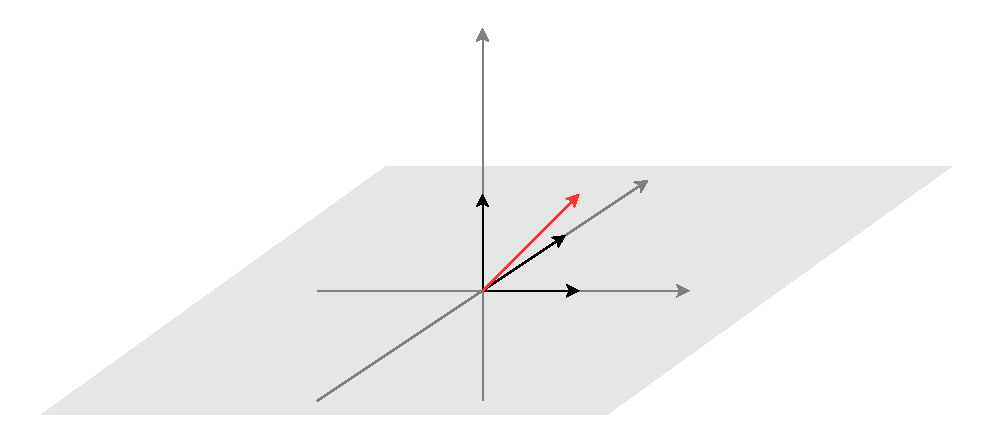
\includegraphics[width=1\linewidth]{res/svg/vector.drawio}
     \caption{Vector in $\mathcal{B}$}
   \end{minipage}\hfill
   \begin{minipage}{0.5\textwidth}
     \centering
     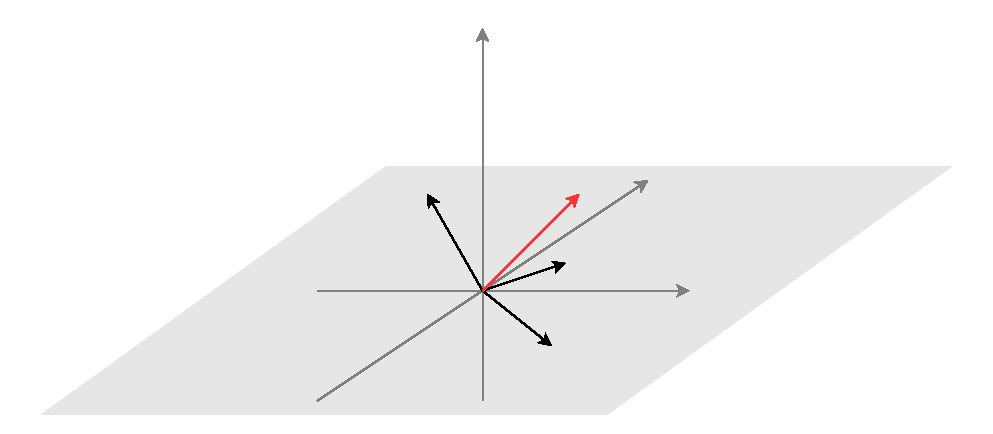
\includegraphics[width=1\linewidth]{res/svg/vettore_new.drawio}
     \caption{Vector in $\mathcal{B}'$}
   \end{minipage}
\end{figure}
Thus we want to write our equations using tensors in the form:
\begin{equation}
  \text{Tensor} = ( \,\dots\, )\;\text{Tensor}
\end{equation}
Lets now dive into more detail and see what types of tensors exist.
\subsection{Order 0 tensors: Scalar fields}
Scalar quantities are invariant under a change of coordinates, for example phase is a scalar field and thus it is invariant:
\begin{equation}
  \phi \longrightarrow \phi' = \phi
\end{equation}
\subsection{Order 1 tensors}
There are two types of order 1 tensors, the first ones are called \textbf{4-vectors}. But what are the prototypes of 4-vectors? As we said we want to obtain a new 4-vector by multipling it by something, in this case the Lorentz matrix $\lm$. If we simply take the vector:
\begin{equation}
  \begin{pNiceMatrix}
    x^0 \\[8pt]
    x^1 \\[8pt]
    x^2 \\[8pt]
    x^3
  \end{pNiceMatrix}
\end{equation}
as the base for our transformations we encounter a problem. If we make a transformation in the Poincarè group the transformations of the coordinates are no longer homogeneous, and so we cannot express the transformation as a simple matrix multiplication, instead we avoid this problem by using the differentials of the coordinates and so our prototype of a 4-vector will be:
\begin{equation}
  \begin{pNiceMatrix}
    \diff{x^0} \\[8pt]
    \diff{x^1} \\[8pt]
    \diff{x^2} \\[8pt]
    \diff{x^3}
  \end{pNiceMatrix}
\end{equation}
And so we will call a 4-vector anything that transforms like $\diff{x^{\mu}}$:
\begin{equation}
  \diff{x'^{\mu}} = \pdv{x'^{\mu}}{x^{\nu}} \diff{x^{\nu}}
\end{equation}
Recall that the elements $\pdv{x'^{\mu}}{x^{\nu}}$ are the elements of the Lorentz matrix and so they can be written as:
\begin{equation}
  \pdv{x'^{\mu}}{x^{\nu}} = \lm^{\mu}_{\nu}
\end{equation}
Leading to the transformations equations of a 4-vector in the desired form:
\begin{equation}
  \boxed{\diff{x'^{\mu}} = \lm^{\mu}_{\nu} \diff{x^{\nu}}}
\end{equation}
Finally we can say:
\begin{equation}
  \tensor{A}{^{\mu}} \text{ is a 4-vector } \iff A'^{\mu} = \lm^{\mu}_{\nu} \tensor{A}{^{\nu}}
\end{equation}
We also call those tensors \textbf{contravariant vectors}.\\
The second type of order 1 tensors are called covariant vectors or \textbf{covectors}. Let's take the four gradient of a scalar field:
\begin{equation}
  \pdv{\phi}{x'^{\mu}}
\end{equation}
By applying the chain rule we have:
\begin{equation}
  \pdv{\phi}{x'^{\mu}} = \pdv{\phi}{x^{\mu}}\pdv{x^{\mu}}{x'^{\mu}}
\end{equation}
But the elements $\pdv{x^{\mu}}{x'^{\mu}}$ are the elements of the inverse Lorentz matrix $\lm^{-1}$ and thus the transformation can be written as:
\begin{equation}
  \pdv{\phi}{x'^{\mu}} = \brackets{\lm^{-1}}^{\nu}_{\mu} \pdv{\phi}{x^{\mu}}
\end{equation}
\subsection{Higher order tensors}
For higher order tensors the transformation is generated by the same amount of matrices as the order, for example an order 2 tensor can transform as follows:
\begin{equation}
  \tensor{F}{^{\prime}^\mu^\nu} = \tensor{\lm}{^{\mu}_{\alpha}}\tensor{\lm}{^{\nu}_{\beta}}F^{\alpha\beta}
\end{equation}
And so, in general, any index trasnforms with its corresponding Lorentz matrix. The same is of course valid for lower indeces and so this generates different cases:
\begin{itemize}
  \item Contravariant tensor of order 2:
  \begin{equation}
    \tensor{F}{^{\prime}^\mu^\nu} = \tensor{\lm}{^{\mu}_{\alpha}}\tensor{\lm}{^{\nu}_{\beta}}F^{\alpha\beta}
  \end{equation}
  \item Covariant tensor of order 2:
  \begin{equation}
    \tensor{F}{^{\prime}_\mu_\nu} = \brackets{\lm_{\mu}^{-1}}^{\alpha}\brackets{\lm_{\mu}^{-1}}_{\nu}^{\beta}F_{\alpha\beta}
  \end{equation}
  \item Mixed tensor of order 2:
  \begin{equation}
    \tensor{F}{^{\prime}^{\mu}_{\nu}} = \tensor{\lm}{^{\mu}_{\alpha}}\brackets{\lm_{\mu}^{-1}}_{\nu}^{\beta}F^{\alpha}_{\beta}
  \end{equation}
\end{itemize}
An example of a mixed tensor is the unit tensor:
\begin{equation}
  \delta^{\mu}_{\nu} \defineeq \begin{cases}
    1 \quad \text{if $\mu = \nu$} \\[8pt]
    0 \quad \text{if $\mu \neq \nu$}
  \end{cases}
\end{equation}
Which has the property:
\begin{equation}
  \begin{split}
    \tensor{A}{^{\mu}} = \delta^{\mu}_{\nu} \tensor{A}{^{\nu}} \\[8pt]
    \tensor{A}{_{\nu}} = \delta^{\mu}_{\nu} \tensor{A}{_{\mu}}
  \end{split}
\end{equation}
The unit tensor can also be represented in matrix form as:
\begin{equation}
  \begin{pNiceMatrix}
    1 & 0 & 0 & 0 \\[8pt]
    0 & 1 & 0 & 0 \\[8pt]
    0 & 0 & 1 & 0 \\[8pt]
    0 & 0 & 0 & 1
  \end{pNiceMatrix}
\end{equation}
But what is the difference between a contravariant and a covariant vector? This is not a general rule, but we can think of those entities as follows:
\begin{itemize}
  \item $\tensor{A}{^{\mu}}$ has upper index $\implies$ row index \begin{equation}
    \begin{pNiceMatrix}
      \tensor{A}{^0} \\[8pt] \tensor{A}{^1} \\[8pt] \tensor{A}{^2} \\[8pt] \tensor{A}{^3}
    \end{pNiceMatrix}
  \end{equation}
  \item $\tensor{A}{_{\mu}}$ has lower index $\implies$ column index \begin{equation}
    \begin{pNiceMatrix}
      \tensor{A}{_0} & \tensor{A}{_1} & \tensor{A}{_2} & \tensor{A}{_3}
    \end{pNiceMatrix}
  \end{equation}
  \item $F_{\mu}^{\nu}$ has an upper index which represents a row and a lower index which represents a column
  \item $F_{\mu \nu}$ has both lower indeces and the first one is associated with a row while the second one with a column (this is valid also when both are upper indeces)
\end{itemize}
\section{Metric properties of spacetime}
In the Euclidean space $\mathbb{E}^3$ the distance between two points $A$ and $B$ is simply the 2-norm (also called Euclidean norm) of the vector. For an infinitesimal displacement $\diff{\vec{r}}$ we have:
\begin{equation}
  \begin{split}
    \diff{\vec{r}}^2 &= \diff{x}^2 + \diff{y}^2 + \diff{z}^2 = \diff{\vec{r}} \cdot \diff{\vec{r}} = \\[8pt]
    &= \diff{x}\diff{x} + \diff{y}\diff{y} + \diff{z}\diff{z} = \\[8pt]
    &= \begin{pNiceMatrix}
      \diff{x} & \diff{y} & \diff{z}\diff{z}
    \end{pNiceMatrix}
    \begin{pNiceMatrix}
      \diff{x} \\[8pt] \diff{y} \\[8pt] \diff{z}
    \end{pNiceMatrix} = \\[8pt]
    &= \begin{pNiceMatrix}
      \diff{x} & \diff{y} & \diff{z}
    \end{pNiceMatrix}
    \begin{pNiceMatrix}
      1 & 0 & 0 \\[8pt] 0 & 1 & 0 \\[8pt] 0 & 0 & 1
    \end{pNiceMatrix}
    \begin{pNiceMatrix}
      \diff{x} \\[8pt] \diff{y} \\[8pt] \diff{z}
    \end{pNiceMatrix}
  \end{split}
\end{equation}
So in the definition of distance in the Euclidean space we implicitly used the identity matrix in order to be able to multiply a row vector with a column vector. But there is no actual constrain that should limit us to use only the identity matrix, as a matter of fact this is just a particular case where the identity matrix is used as the \textbf{metric tensor}. In principle we could define infinitely many ways to calculating distance just by changing the metric tensor, but we are interested to what happens in $\mink$. We already defined the distance between two events ad the invariant quantity:
\begin{equation}
  \diff{s}^2 = c^2\diff{t}^2 - \diff{x}^2 - \diff{y}^2 - \diff{z}^2
\end{equation}
And so it is not surprising that the metric tensor in $\mink$ is:
\begin{equation}
  \tensor{g}{_\mu_\nu} \defineeq
  \begin{pNiceMatrix}
    1 & 0 & 0 & 0 \\[8pt]
    0 & -1 & 0 & 0 \\[8pt]
    0 & 0 & -1 & 0 \\[8pt]
    0 & 0 & 0 & -1
  \end{pNiceMatrix}
\end{equation}
And so the infinitesimal distance can also be written as:
\begin{equation}
  \diff{s}^2 =
  \begin{pNiceMatrix}
    \diff{x^0} & \diff{x^1} & \diff{x^2} & \diff{x^3}
  \end{pNiceMatrix}
  \begin{pNiceMatrix}
    1 & 0 & 0 & 0 \\[8pt]
    0 & -1 & 0 & 0 \\[8pt]
    0 & 0 & -1 & 0 \\[8pt]
    0 & 0 & 0 & -1
  \end{pNiceMatrix}
  \begin{pNiceMatrix}
    \diff{x^0} \\[8pt] \diff{x^1} \\[8pt] \diff{x^2} \\[8pt] \diff{x^3}
  \end{pNiceMatrix}
\end{equation}
Or, in tensor notation:
\begin{equation}
  \boxed{\diff{s}^2 = \diff{x}^{\mu} g_{\mu \nu} \diff{x}^{\nu}}
\end{equation}
The metric tensor is an order 2 covariant tensor, and it is invariant under Lorentz transformation:
\begin{equation}
  \tensor{g}{^{\prime}_\mu_\nu} = \tensor{\brackets{\lm^{-1}}}{^{\alpha}_{\mu}} \tensor{\brackets{\lm^{-1}}}{^{\beta}_{\nu}} \tensor{g}{_\alpha_\beta} = \tensor{g}{_\mu_\nu}
\end{equation}
This leads to what is called a \textbf{Pseudo-Riemannian geometry} which is different from Euclidean geometry.\\
From the definition of the metric tensor follows:
\begin{equation}
  \tensor{g}{^\mu^\nu} = \brackets{\tensor{g}{_\mu_\nu}}^{-1} = \tensor{g}{_\mu_\nu}
\end{equation}
So $\tensor{g}{^\mu^\nu} = \tensor{g}{_\mu_\nu}$ and the metric tensor is equal to its inverse. This connects covariant and contravariant tensors with the following relations:
\begin{equation}
  \begin{split}
    \tensor{A}{^{\mu}} = \tensor{g}{_\mu_\nu} \tensor{A}{^{\mu}} = (\,\dots) \tensor{A}{_{\nu}} \\[8pt]
    \tensor{A}{_{\mu}} = \tensor{g}{^\mu^\nu} \tensor{A}{_{\mu}} = (\,\dots) \tensor{A}{^{\nu}}
  \end{split}
\end{equation}
This operation is sometimes also called \textbf{index lowering} and the effect on the components is:
\begin{equation}
  \begin{pNiceMatrix}
    A^0 \\[8pt] A^1 \\[8pt] A^2 \\[8pt] A^3
  \end{pNiceMatrix}
  \longrightarrow
  \begin{pNiceMatrix}
    A_0 & -A_1 & -A_2 & -A_3
  \end{pNiceMatrix}
\end{equation}
So in general the metric tensor $\tensor{g}{_\mu_\nu}$ allows us to lower an index by switching sign to the spatial component $i = 1,2,3$. For example:
\begin{equation}
  \begin{split}
    &\partial_{\mu} \phi \quad \text{is a covector} \\[8pt]
    &\partial^{\mu} \phi \quad \text{is a contravariant vector}
  \end{split}
\end{equation}
And they are connected by the following relation:
\begin{equation}
  \begin{pNiceMatrix}
    \partial^0 \\[8pt] \partial^1 \\[8pt] \partial^2 \\[8pt] \partial^3
  \end{pNiceMatrix}
  \longrightarrow
  \begin{pNiceMatrix}
    \partial_0 & -\partial_1 & -\partial_2 & -\partial_3
  \end{pNiceMatrix}
\end{equation}
\subsection{Magnitude of a 4-vector}
We define the magnitude of a 4-vector in the same way as $\diff{x}^{\mu} \rightarrow \diff{s}^2 = \brackets{\diff{x^0}}^2 - \brackets{\diff{x^1}}^2 - \brackets{\diff{x^2}}^2 - \brackets{\diff{x^3}}^2$. And so we have:
\begin{equation}
  \diff{s}^2 = \diff{x}^{\mu} \tensor{g}{_\mu_\nu} \diff{x}^{\nu} = \diff{x}^{\mu} \diff{x}_{\nu}
\end{equation}
Thus, for a generic tensor:
\begin{equation}
  \boxed{A^2 = A^{\mu} A_{\mu}}
\end{equation}
In fact, if we expand term by term we get:
\begin{equation}
  \begin{split}
    A^2 &= A^{0} A_{0} + A^{1} A_{1} + A^{2} A_{2} + A^{3} A_{3} = \\[8pt]
    &= A^{0} A^{0} - A^{1} A^{1} - A^{2} A^{2} - A^{3} A^{3} = \\[8pt]
    &= \brackets{A^{0}}^2 - \brackets{A^{1}}^2 - \brackets{A^{2}}^2 - \brackets{A^{3}}^2
  \end{split}
\end{equation}
\subsection{Scalar product of a 4-vector}
As we did for the magnitude we can define the scalar product between two tensors as:
\begin{equation}
  x^{\mu} \tensor{g}{_\mu_\nu} q^{\nu} = x^{\mu} q_{\mu} = x^{0} q^{0} - x^{1} q^{1} - x^{2} q^{2} -x^{3} q^{3}
\end{equation}
The condition of orthogonality follows from the definition of the scalar product:
\begin{equation}
  x^{\mu} \text{ is orthogonal to } q^{\nu} \iff x^{\mu} q_{\mu} = 0
\end{equation}
\section{Other properties}
The partial derivative of a tensor with respect to the coordinates is not, in general, a tensor.
\begin{equation}
  A^{\mu} \longrightarrow \pdv{A^{\mu}}{x^{\nu}}
\end{equation}
But if it was a tensor it would transform as an order 2 tensor (2 indices) with the matrices $\lm$ and $\lm^{-1}$. Lets see what happens:
\begin{equation}
  \pdv{A'^{\mu}}{x'^{\nu}} = \pdv{\brackets{\tensor{\lm}{_{\alpha}^{\mu}} A^{\mu}}}{x'^{\nu}}
\end{equation}
Since $\tensor{\lm}{_{\alpha}^{\mu}}$ does not depend on the coordinates its partial derivative is zero:
\begin{equation}
  \pdv{A'^{\mu}}{x'^{\nu}} = \tensor{\lm}{^{\mu}_{\alpha}} \pdv{A^{\mu}}{x'^{\nu}} = \tensor{\lm}{^{\mu}_{\alpha}} \pdv{A^{\mu}}{x^{\beta}}\pdv{x^{\beta}}{x'^{\nu}}
\end{equation}
But $\pdv{x^{\beta}}{x'^{\nu}}$ are the elements of $\tensor{\brackets{\lm^{-1}}}{^{\beta}_{\nu}}$ so we finally get:
\begin{equation}
  \pdv{A'^{\mu}}{x'^{\nu}} = \tensor{\lm}{^{\mu}_{\alpha}} \tensor{\brackets{\lm^{-1}}}{^{\beta}_{\nu}} \pdv{A^{\mu}}{x^{\beta}}
\end{equation}
This is how a mixed tensor transforms, so for Lorentz transformations the derivative of a tensor is still a tensor.\\
Another property of 4-vectors in $\mink$ is that they have a time component and 3 space components, so the lowering of an index can be obtained by just switching sign to the space associated vector:
\begin{equation}
  A^{\mu} = \brackets{A^0, \vec{A}} \rightarrow A_{\mu} = \brackets{A^0, -\vec{A}}
\end{equation}

\chapter{Representation of spacetime}
\section{Spacetime diagrams}
Now we will discuss the representation of spacetime with diagrams. Let's start from some basic concepts.\\
In a spacetime diagram an object that stays at rest is just an object with fixed spatial coordinates at any given time. This defines what is called a \textbf{world line}:
\begin{figure}[H]
  \centering
  \includegraphics[width=0.8\linewidth]{res/svg/World_line.drawio}
\end{figure}
Instead an object moving in space has a space trajectory, which is the projection of the spacetime path onto the spatial coordinates, instead it must always increase in the time direction, giving a diagram of this type:
\begin{figure}[H]
  \centering
  \includegraphics[width=0.8\linewidth]{res/svg/spacetime_path.drawio}
\end{figure}
Now we need to focus our attention on the limitations on the possible timepaths. For an infinitesimal displacement in space the object travels with velocity $u$ which must be lower then $c$, this means that the angle of the line tangent to the path is limited. We can represent the situation as:
\begin{figure}[H]
  \centering
  \includegraphics[width=0.8\linewidth]{res/svg/spacetime_angle.drawio}
\end{figure}
The tangent of $\psi$ is:
\begin{equation}
  \tan \psi = \dfrac{u}{c}
\end{equation}
For an object with mass this quantity is obviously limited by $1$ and so:
\begin{equation}
  \tan \psi < 1 \implies \psi < \qty{45}{\degree}
\end{equation}
And so any spacetime path of an object with mass is limited by a maximum angle of the tangent line equal to $\qty{45}{\degree}$. This identifies a well known geometric shape in the spacetime diagram which is called \textbf{light cone}:
\begin{figure}[H]
  \centering
  \includegraphics[width=0.8\linewidth]{res/svg/light_cone.drawio}
\end{figure}
Instead if we look at the spacetime path of a light beam it must be on the surface of the cone.\\
The light cone also divides spacetime in different regions.
\section{Events}
\subsection{Time-like events}
An event inside the cone must be such that:
\begin{equation} \label{e:timelike_condition}
  \norm{\Delta \vec{r}} < \Delta x^0
\end{equation}
But $\Delta x^0 = c\Delta t$ which means that:
\begin{equation}
  \dfrac{\norm{\Delta \vec{r}}}{\Delta t} < c
\end{equation}
So this event is in the \textbf{future} for the IRF. Equation \eqref{e:timelike_condition} also leads to:
\begin{equation}
  \Delta s^2 = \Delta x^0 - \norm{\Delta \vec{r}} > 0
\end{equation}
An event with $\Delta s^2 > 0$ is called \textbf{time-like}. If $\Delta x^0 < 0$ but $\norm{\Delta \vec{r}} < \abs{\Delta x^0}$ the event is still time-like, but it is in the past for the IRF.
\subsection{Space-like events}
Similarly, an event outside the cone is such that:
\begin{equation} \label{e:spacelike_condition}
  \norm{\Delta \vec{r}} > \Delta x^0
\end{equation}
But $\Delta x^0 = c\Delta t$ which means that:
\begin{equation}
  \norm{\Delta \vec{r}} > c\Delta t
\end{equation}
So there is no way a signal from the origin could travel fast enough to reach the point where the event will happen. This means that the event cannot be caused by something in the origin. This was also the condition necessary in order to be able to find a moving IRF such that the time order of the event is swapped.
In general an event with these properties satisfies:
\begin{equation}
  \Delta s^2 = \Delta x^0 - \norm{\Delta \vec{r}} < 0
\end{equation}
And is called \textbf{space-like event}.\\
The region outside the cone is called \textbf{undetermined present}.\\

\chapter{Classical quantities in Special Relativity}
\section{4-velocity}
In classical mechanics the velocity of a particle is:
\begin{equation}
  \vec{u} = \dv{\vec{r}}{t}
\end{equation}
This still holds in Relativity, but only for the spatial coordinates, so we must choose something that is invariant to define the 4-velocity tensor.
We know that $\diff{s}^2$ is invariant so let's introduce another invariant quantity based on this:
\begin{equation}
  \diff{\tau}^2 = \dfrac{\diff{s}^2}{c^2}
\end{equation}
First we can notice that $\sqbr{\diff{\tau}} = \sqbr{s}$ and if we expand $\diff{\tau}^2$ from its definition:
\begin{equation}
  \begin{split}
    \diff{\tau}^2 &= \diff{t}^2 - \dfrac{\norm{\diff{\vec{r}}}^2}{c^2} =\\[8pt]
    &= \diff{t}^2 \brackets{1 - \dfrac{u^2}{c^2}} = \dfrac{\diff{t}^2}{\gamma^2(u)}
  \end{split}
\end{equation}
So $\diff{\tau} = \dfrac{\diff{t}}{\gamma(u)}$. If we choose the IRF of istantaneous rest, also called \textbf{co-moving IRF} we have that $\diff{\tau}$ is:
\begin{equation}
  \diff{\tau} = \dfrac{\diff{t}}{\gamma(0)} = \diff{t}
\end{equation}
Thus, $\diff{\tau}$ is the $\diff{t}$ evaluated in the IRF in which the particle is at rest and is the proper time interval.\\
Let's go back to our original problem and define the 4-velocity tensor as:
\begin{equation}
  u^{\mu} = \dv{x^{\mu}}{\tau}
\end{equation}
The tensor $u^{\mu}$ is contravariant. Now, by applying the chain rule we get:
\begin{equation}
  u^{\mu} = \dv{x^{\mu}}{\tau} = \dv{x^{\mu}}{t} \dv{t}{\tau} =\gamma(u) \dv{x^{\mu}}{t}
\end{equation}
Now we exploit the definiton of $\diff{x}^{\mu} = \brackets{c\diff{t}, \diff{\vec{r}}}$ leading to:
\begin{equation}
  \boxed{u^{\mu} = \gamma(u) \brackets{c, \vec{u}}}
\end{equation}
Now we should ask ourselves what the magnitude of the 4-velocity is. By using the definition of magnitude we have established we get:
\begin{equation}
  u^2 = u^{\mu}u_{\mu} = \gamma^2(u)\brackets{c^2 - u^2} = \cancel{\gamma^2(u)}c^2\cancel{\brackets{1 - \dfrac{u^2}{c^2}}} = c^2
\end{equation}
So the magnitude of the 4-velocity will always be $c$. Even for an object at rest we have:
\begin{equation}
  u^{\mu} = \gamma(u)\brackets{c, \vec{u}} = \gamma(0)\brackets{c, \vec{0}} = \brackets{c, \vec{0}}
\end{equation}
And so the magnitude is indeed $c$. Now let us see what happens if we apply a Lorentz transformation to $\tensor{u}{^\mu} \rightarrow \tensor{u}{^\prime^\mu} = \tensor{\lm}{^\mu_\nu}\tensor{u}{^\nu}$:
\begin{equation}
  \tensor{u}{^\prime^\mu} =
  \begin{cases}
    \tensor{u}{^\prime^0} = \gamma \left( u^{0} - \dfrac{v}{c} u^{1} \right) \\[8pt]
    \tensor{u}{^\prime^1} = \gamma \left( u^{1} -  \dfrac{v}{c} u^{0}\right) \\[8pt]
    \tensor{u}{^\prime^2} = u^{2} \\[8pt]
    \tensor{u}{^\prime^3} = u^{3}
  \end{cases} =
  \begin{cases}
    \tensor{u}{^\prime^0} = \gamma \left( \gamma(u)c - \dfrac{v}{c} \gamma(u)u_x \right) \\[8pt]
    \tensor{u}{^\prime^1} = \gamma \left( \gamma(u)u_x -  \dfrac{v}{c} \gamma(u)c \right) \\[8pt]
    \tensor{u}{^\prime^2} = u^{2} \\[8pt]
    \tensor{u}{^\prime^3} = u^{3}
  \end{cases}
\end{equation}
After some calculations the first transformation leads to:
\begin{equation} \label{gamma_transformation}
  \dfrac{\gamma(u')}{\gamma(u)} = \gamma(v)\brackets{1-\dfrac{v u_x}{c^2}}
\end{equation}
From the second we get:
\begin{equation}
  \dfrac{\gamma(u')}{\gamma(u)}\tensor{u}{^\prime_x} = \gamma(v)\brackets{u_x - v}
\end{equation}
And so putting those equations together we have:
\begin{equation}
  \begin{split}
    \cancel{\gamma(v)}\brackets{1-\dfrac{v u_x}{c^2}}\tensor{u}{^\prime_x} = \cancel{\gamma(v)}\brackets{u_x - v} \\[8pt]
    \tensor{u}{^\prime_x} = \dfrac{u_x - v}{1-\dfrac{v u_x}{c^2}}
  \end{split}
\end{equation}
And we aslo obtain the relation:
\begin{equation}
  \gamma(u') = \dfrac{\gamma(u)\gamma(v)\brackets{u_x-v}}{\tensor{u}{^\prime_x}}
\end{equation}
Now the third transformation is simply:
\begin{equation}
  \gamma(u')\tensor{u}{^\prime_y} = \gamma(u)\tensor{u}{_y}
\end{equation}
Substituting the relation for $\gamma(u')$ gives:
\begin{equation}
  \begin{split}
    \dfrac{\cancel{\gamma(u)}\gamma(v)\brackets{u_x-v}}{\tensor{u}{^\prime_x}}\tensor{u}{^\prime_y} = \cancel{\gamma(u)}\tensor{u}{_y} \\[8pt]
    \tensor{u}{^\prime_y} = \dfrac{\tensor{u}{^\prime_x} \tensor{u}{_y}\sqrt{1-\dfrac{v^2}{c^2}}}{u_x-v}
  \end{split}
\end{equation}
\section{4-acceleration}
Similarly to what we did for the velocity we want to define a tensor for the acceleration. We define:
\begin{equation}
  a^{\mu} = \dv{u^{\mu}}{\tau} = \dv{u^{\mu}}{t}\dv{t}{\tau} = \gamma(u)\dv{u^{\mu}}{t}
\end{equation}
And so we have:
\begin{equation}
  \begin{split}
    a^{\mu} &= \gamma(u)\brackets{\dv{\brackets{\gamma(u)c}}{t}, \dv{\brackets{\gamma(u)\vec{u}}}{t}} = \\[8pt]
    &= \gamma(u)\brackets{c\dot{\gamma}(u), \dot{\gamma}(u)\vec{u} + \gamma(u)\vec{a}}
  \end{split}
\end{equation}
We can notice that the 4-acceleration $a^{\mu}$ is zero if and only if the vectorial acceleration $\vec{a}$ is zero. In fact if $u$ is constant:
\begin{equation}
  a^{\mu} = \gamma^2(u)\brackets{0,\vec{a}}
\end{equation}
In the co-moving IRF we additionally have that $\gamma(0) = 1$:
\begin{equation}
  a^{\mu} = \brackets{0,\vec{a}}
\end{equation}
Is the relation of orthogonality conserved for the 4-acceleration and the 4-velocity? The answer is yes and it can be shown knowing that the magnitude of any 4-velocity is constant and equal to $c$:
\begin{equation}
  \dv{c^2}{t} = 0 \implies \dv{\brackets{u^{\mu}u_{\mu}}}{t} = 0
\end{equation}
But if we perform the derivative:
\begin{equation}
  \begin{split}
    \dot{u}^{\mu}u_{\mu} + u^{\mu}\dot{u}_{\mu} = 0 \\[8pt]
    \dot{u}^{\mu}u_{\mu} + u_{\mu}\dot{u}^{\mu} = 0 \\[8pt]
    \boxed{a^{\mu}u_{\mu} = 0}
  \end{split}
\end{equation}
Notice that we raised and lowered an index in the second term of the expression and so this does not change any sign.\\
The square magnitude of $a^{\mu}$ is:
\begin{equation}
  a_{\mu}a^{\mu} = \begin{pNiceMatrix}
    0 & \vec{a}
  \end{pNiceMatrix}
  \begin{pNiceMatrix}
    0 \\ -\vec{a}
  \end{pNiceMatrix} = -a^2
\end{equation}
So the 4-velocity is a spacelike vector, instead the 4-acceleration is a timelike vector.\\
After defining the 4-velocity and the 4-acceleration we are ready to start talkin about dynamics in Special Relativity. In classical mechanics we have some fundamental principles:
\begin{itemize}
  \item Newton's \nth{1} law: Inertia
  \item Newton's \nth{2} law: $\sum \vec{F} = m\vec{a}$
  \item Newton's \nth{3} law
  \item Conservation laws
\end{itemize}
Inertia still holds in general relativity, but the Newton's \nth{2} law must not be true since we have a limit to the speed that a moving object can reach. Also Newton's \nth{3} law is not, in general true, but it still holds for contact forces. Conservation laws are still true.
\section{Mass}
In classical mechanics we essentially defined 3 types of masses:
\begin{itemize}
  \item[a.] Proper mass, which is the one measured in the IRF at rest
  \item[b.] Inertial mass
  \item[c.] Gravitational mass
\end{itemize}
In principle there is no reason for the gravitational mass to be the same as the inertial mass, but they are found to be numerically identical and so in classical mechanics $a = b = c$. In Special Relativity this relation is no longer true, we only have that $b = c$, but $a \neq b$ and $a \neq c$.\\
In Relativity mass at rest is not the same as mass in motion, in fact if we want a relation of the kind $\vec{F} = m\vec{a}$ to be true we need an acceleration that decreases in order to avoid reaching the speed of light, but we also need an increasing mass to balance the effect of the acceleration.\\
Imagine we shoot a projectile in the $y$ direction that enters a wall for a distance $d$, which is proportional to the momentum of the particle $p_y = m(u_y)u_y$ in another moving IRF we see $d=d'$ this implies that $p_y = p'_y$. We choose $u_x = v$ and, from the equations of transformations of the velocities we get:
\begin{equation}
  \begin{split}
    m(u_y)u_y &= m(u'_y)u'_y \\[8pt]
    m(u_y)\cancel{u_y} &= m(u'_y)\dfrac{\cancel{u_y}\sqrt{1-\dfrac{v^2}{c^2}}}{1-\dfrac{u_x v}{c^2}} \\[8pt]
    m(u_y) &= m(u'_y)\dfrac{\sqrt{1-\dfrac{v^2}{c^2}}}{1-\dfrac{v^2}{c^2}} \\[8pt]
    m(u'_y) &= \dfrac{m(u_y)}{\gamma(v)}
  \end{split}
\end{equation}
Now from equation \eqref{gamma_transformation} we have:
\begin{equation}
  \dfrac{\gamma(u')}{\gamma(u)} = \gamma(v)\brackets{1-\dfrac{v u_x}{c^2}} = \dfrac{1}{\gamma(v)}
\end{equation}
Substituting back we get:
\begin{equation}
  \begin{split}
    m(u') = m(u)\dfrac{\gamma(u')}{\gamma(u)} \\[8pt]
    \boxed{\dfrac{m(u'_y)}{\gamma(u')} = \dfrac{m(u_y)}{\gamma(u)}}
  \end{split}
\end{equation}
And so we found out that the quantity $m/ \gamma$ is invariant and so we define:
\begin{equation}
  m_0 \defineeq \dfrac{m(0)}{\gamma(0)} = m(0)
\end{equation}
This is the \textbf{proper mass}, which is the mass measured at rest. Given this we can find the value of mass as a function of the velocity:
\begin{equation}
  m = m_0\gamma(u)
\end{equation}
\section{4-momentum}
We can define the 4-momentum in similarity to the classical case:
\begin{equation}
  p^{\mu} = m_0 u^{\mu}
\end{equation}
But from our definition of the 4-velocity tensor we have:
\begin{equation}
  p^{\mu} = m_0 u^{\mu} = m_0 \gamma(u)\brackets{c, \vec{u}} = \brackets{mc, m\vec{u}} = \brackets{mc, \vec{p}}
\end{equation}
The square magnitude of this tensor can be easily obtained from the magnitude of the 4-velocity:
\begin{equation}
  p_{\mu}p^{\mu} = m_0^2u_{\mu}u^{\mu} = m_0^2c^2 = p^2
\end{equation}
We define $p^2$ as this, but it is not equal to the square modulus of the vector $\vec{p}$, in order to avoid confusion the square magnitude of only the spatial part will be noted as $\vec{p}^2$.
\subsection{Energy}
In Special Relativity we define energy with the famous equation:
\begin{equation}
  E \defineeq mc^2
\end{equation}
We can see that for $u \ll c$ we can do a Taylor expansion of $m$ to the first order and obtain:
\begin{equation}
  m = m_0\brackets{1-\dfrac{u^2}{c^2}}^{-1/2} \sim m_0\brackets{1+\dfrac{1}{2}\dfrac{u^2}{c^2}}
\end{equation}
And so energy becomes:
\begin{equation}
  E \sim m_0c^2 + \dfrac{1}{2}m_0u^2
\end{equation}
We can distinguish two different terms:
\begin{itemize}
  \item The \textbf{rest energy} $E_0 = m_0c^2$
  \item The classical kinetic energy $T = \dfrac{1}{2}m_0u^2$
\end{itemize}
The term $E_0$ is associated to the mass itself and so, even at rest, any mass is associated to a minimum value of energy. The value of $E_0$ might change, for example if we keep a system still, but raise the energy by warming it, the energy $E_0$ raises and so the mass $m_0$ must go up aswell. Viceversa is also true, an example is given by nuclear reactions where the ``lost mass'' is converted to energy. Since the proportionality constant is $c^2$ it is dramatically easier to obtain energy from mass and not the opposite, this is why nuclear reactions can produce a lot of energy with relatively small quantities of fuel.\\
Now we want to focus our attention on the kinetic energy term. The equivalence we got with the classical case is only valid in the limit of small velocities, in general we define the kinetic energy as the total energy minus the potential energy (in this case the rest energy).
\begin{equation}
  T = E - V = m_0\gamma(u)c^2 - m_0c^2 = m_0c^2\brackets{\gamma(u)-1}
\end{equation}
After this brief discussion about energy we can define in an alternative way the 4-momentum as:
\begin{equation}
  p^{\mu} = \brackets{\dfrac{E}{c}, \vec{p}}
\end{equation}
Notice that this definition does not contain mass anymore in the first term, this will be useful in just a moment.\\
Let us calculate again $p_{\mu}p^{\mu}$:
\begin{equation}
  p_{\mu}p^{\mu} = \dfrac{E^2}{c^2} - \vec{p}^2 = m_0c^2
\end{equation}
And so we get an alternative definiton of energy:
\begin{equation}
  \begin{split}
    &\dfrac{E^2}{c^2} - \vec{p}^2 = m_0c^2 \\[8pt]
    &E^2 = \vec{p}^2c^2 + m_0c^4 \\[8pt]
    &E = \sqrt{\vec{p}^2c^2 + m_0c^4}
  \end{split}
\end{equation}
This is a very important formula and is the base to solve many problems in Special Relativity.\\
In Relativity we just ask for this condition:
\begin{equation}
  p^{\mu}_f = p^{\mu}_i
\end{equation}
Which implies that:
\begin{equation}
  \begin{split}
    E_f = E_i \\[8pt]
    \vec{p}_f = \vec{p}_i
  \end{split}
\end{equation}
\subsection{Photons}
Since photons travel at speed $c$ they must be massless ($m_0 =0$). Actually it does not even make sense to define a mass for photons since, by definition, there is no IRF where light is at rest. We also know that the energy of a photon is $E = h\nu$, from the equation of energy we just got we have:
\begin{equation}
  E = \sqrt{\vec{p}^2c^2 + 0} = \norm{\vec{p}}c
\end{equation}
From this we can easily get the same results we previously got for the Relativistic Doppler effect. We have that:
\begin{equation}
  \begin{split}
    p'^{\mu} = \brackets{\dfrac{h\nu_s}{c}, \dfrac{h\nu_s}{c}\cos \theta_s, \dfrac{h\nu_s}{c}\sin \theta_s, 0} \\[8pt]
    p^{\mu} = \brackets{\dfrac{h\nu_r}{c}, \dfrac{h\nu_r}{c}\cos \theta_r, \dfrac{h\nu_r}{c}\sin \theta_r, 0}
  \end{split}
\end{equation}
We know that we need to get $p'^{\mu}$ after applying the inverse Lorentz matrix to $p^{\mu}$:
\begin{equation}
  \begin{pNiceMatrix}
    \gamma & \gamma \beta & 0 & 0 \\[8pt]
    \gamma \beta & \gamma & 0 & 0 \\[8pt]
    0 & 0 & 1 & 0 \\[8pt]
    0 & 0 & 0 & 1
  \end{pNiceMatrix}
  \begin{pNiceMatrix}
    \nu_r \\[8pt] \nu_r \cos \theta_r \\[8pt] \nu_r \sin \theta_r \\[8pt] 0
  \end{pNiceMatrix}
  \cancel{\dfrac{h}{c}}
  = \cancel{\dfrac{h}{c}}\begin{pNiceMatrix}
    \nu_s \\[8pt] \nu_s\cos \theta_s \\[8pt] \nu_s\sin \theta_s \\[8pt] 0
  \end{pNiceMatrix}
\end{equation}
This is a simple non homogeneous linear system which gives us:
\begin{equation}
  \begin{cases}
    \nu_r = \gamma \nu_s\brackets{1 + \beta \cos \theta_s} \\[8pt]
    \nu_r\cos \theta_r = \gamma \nu_s\brackets{\beta + \cos \theta_s} \\[8pt]
    \nu_r\sin \theta_r = \nu_s\sin \theta_s
  \end{cases}
\end{equation}
And those are exactly the equations we got with our reasoning about phase invariance (the last equation was not included since it is essentially useless $0 = 0$).
\section{4-Force}
We define the 4-force as:
\begin{equation}
  F^{\mu} = \dv{p^{\mu}}{\tau} = \dv{p^{\mu}}{t} \dv{t}{\tau} = \gamma (u)\dv{p^{\mu}}{t}
\end{equation}
In this case $u$ is the speed of the object when $\vec{F}$ is applied. We also have that:
\begin{equation}
  F^{\mu} = \gamma(u)\dv{}{t}\brackets{cm, \vec{p}} = \gamma(u) \brackets{c\dv{m}{t}, \vec{F}}
\end{equation}
Now we can see that $F^{\mu}$ is related to the 4-acceleration because of this relation:
\begin{equation}
  F^{\mu} = \dv{p^{\mu}}{\tau} = \dv{\brackets{m_0u^{\mu}}}{\tau} = m_0\dv{u^{\mu}}{\tau} = m_0 a^{\mu}
\end{equation}
So we have that:
\begin{equation}
  \brackets{c \dv{m}{t}, \vec{F}} = m_0\brackets{\dot{\gamma}c, \dot{\gamma}\vec{u} + \gamma\vec{a}}
\end{equation}
Which gives:
\begin{equation}
  \vec{F} = m_0\brackets{\dot{\gamma}\vec{u} + \gamma\vec{a}}
\end{equation}
Also the orthogonality of $F^{\mu}$ and $u^{\mu}$ follows from the orthogonality of the 4-velocity and the 4-acceleration:
\begin{equation}
  F_{\mu}u^{\mu} = m_0 a_{\mu}u^{\mu} = 0
\end{equation}
Calculating this excplicitly gives:
\begin{equation}
  \begin{split}
    \gamma \begin{pmatrix}
    c \dv{m}{t} & -\vec{F}
  \end{pmatrix} \gamma \begin{pmatrix}
    c \\ \vec{u}
  \end{pmatrix} = \\[8pt]
    \gamma^2 \brackets{c^2 \dv{m}{t} - \vec{F}\cdot\vec{u}} = 0
  \end{split}
\end{equation}
The parenthesis gives:
\begin{equation} \label{e:F_dmdt_equivalence}
  \dfrac{\vec{F}\cdot\vec{u}}{c} = c \dv{m}{t}
\end{equation}
The term $\vec{F}\cdot\vec{u}$ has the dimension of power and substituting in the general formula for the 4-force gives:
\begin{equation}
  F^{\mu} = \brackets{\dfrac{\vec{F}\cdot\vec{u}}{c}, \vec{F}}
\end{equation}
Now we need to find the relation between the classical vectors $\vec{F}$ and $\vec{a}$. We know that:
\begin{equation}
  \cancel{\gamma} \vec{F} = \cancel{\gamma} \dv{}{t}\brackets{m\vec{u}}
\end{equation}
From this, exploiting \eqref{e:F_dmdt_equivalence} we arrive to:
\begin{equation}
  \begin{split}
    \vec{F} &= \dv{}{t}\brackets{m\vec{u}} \\[8pt]
    &= \dv{m}{t}\vec{u} + m\vec{a} = \\[8pt]
    &= \dfrac{\vec{F}\cdot\vec{u}}{c^2}\vec{u} + m\vec{a}
  \end{split}
\end{equation}
And so, in general, $\vec{F}$ is not parallel to $\vec{a}$ in Special Relativity, but we have some exceptions:
\begin{itemize}
  \item $\vec{u} = \vec{0}$
  \item $\vec{F}\cdot\vec{u} = 0 \implies \vec{F} \perp \vec{u}$ (for example in cyclotronic motion)
  \item $\vec{u} \parallel \vec{a}$
\end{itemize}
Recalling the vector transformation of the position $\vec{r}$ we can get to the vector Lorentz transformation of the force $\vec{F}$. The calculation is long, we just give the result:
\begin{equation}
  \vec{F}' = \dfrac{\dfrac{\vec{F}}{\gamma (v)} + \vec{v}\sqbr{\brackets{1- \dfrac{1}{\gamma(v)}}\dfrac{\vec{v}\cdot \vec{F}}{v^2}-\dfrac{\vec{F}\cdot \vec{u}}{c^2}}}{1-\dfrac{\vec{v}\cdot\vec{u}}{c^2}}
\end{equation}
If $\vec{u} \parallel \vec{v} \rightarrow (u, 0, 0) \parallel (v, 0, 0)$ we have:
\begin{equation}
  \begin{split}
    F'_x = F_x \\[8pt]
    F'_y = \dfrac{F_y}{\gamma(v)\brackets{1-\dfrac{uv}{c^2}}}\\[8pt]
    F'_z = \dfrac{F_z}{\gamma(v)\brackets{1-\dfrac{uv}{c^2}}}
  \end{split}
\end{equation}
\section{Examples (WIP)}
\subsection{Ex.1} (TO DO)\\
\subsection{Ex.2} (TO DO)\\
\subsection{Ex.3} (TO DO)\\
\subsection{Ex.4} (TO DO)\\

\chapter[Relativistic EM]{Relativistic formulation of electromagnetism}
\section{Charge invariance}
Let us now discuss the formulation of electromagnetism in the relativistic framework. First off we start with stating a property:
\begin{quotation}
  The charge of a particle is independent of its velocity, thus it is Lorentz invariant
\end{quotation}
This makes sense since Maxwell's equations (in contrary to Newton's equations) are already Lorentz invariant.\\
As an example we take a volume $V$ at rest in an IRF $\irf{R}$ that contains $N$ elementary particles of charge $e$. The total charge inside the volume is:
\begin{equation}
  Q = Ne
\end{equation}
But we can also describe the total charge in terms of the charge density $\rho$:
\begin{equation}
  Q = \rho V = n e V
\end{equation}
Where $n$ is the number of charges per unit volume in the reference frame. If we take a second IRF $\irf{R}'$ in motion with respect to the first one we have:
\begin{equation}
  Q' = \rho'V' = n'eV'
\end{equation}
Since we stated that the total charge must be the same in all IRFs we have:
\begin{equation}
  n e V = n'eV'
\end{equation}
We have that the volume transforms as $V' = \dfrac{V_0}{\gamma(v)}$ where $V_0$ is the volume measured at rest which means that $V = V_0$. Thus we get:
\begin{equation}
  \begin{split}
    n \cancel{V_0} &= n' \dfrac{\cancel{V_0}}{\gamma(v)} \\[8pt]
    n' &= n\gamma(v)
  \end{split}
\end{equation}
This means that we see more charges per unit volume in the moving IRF, which makes sense if we think that the number of charges is the same but the volume is ``squeezed'' by the effect of lenght contraction.\\ The same is true for the charge density:
\begin{equation}
  \boxed{\rho' = \rho_0 \gamma(v)}
\end{equation}
Where $\rho_0$ is the proper charge density, measured in the IRF where the volume is at rest. We can also notice that $\rho$ transforms as $\diff{x^0}$.\\
The infinitesimal charge is also invariant and so also the following quantity is invariant:
\begin{equation}
  \diff{q} = \rho \diff{V}
\end{equation}
But also the infinitesimal volume in 4 dimensions is invariant, in fact we just have that:
\begin{equation}
  \diff{^4x} = \diff{x^0}\diff{x^1}\diff{x^2}\diff{x^3}
\end{equation}
Which transforms with:
\begin{equation}
  \diff{^4x'} = \det \lm \diff{x'^0}\diff{x'^1}\diff{x'^2}\diff{x'^3}
\end{equation}
The determinant of the Lorentz matrix is essentially the contribution of the Jacobian in any change of variable, but we previously got that the determinat of the Lorentz matrix is $1$ so:
\begin{equation}
  \diff{^4x'} = \diff{^4x}
\end{equation}
\section{Potentials}
We need to define a current density tensor. Could $J^{\mu} = \brackets{\rho, \vec{J}}$ be a good candidate? The answer is no, since the tensor would have quantities of different dimensions, but it turns out that $J^{\mu} = \brackets{\rho c, \vec{J}}$ works just fine as we will now see.\\
We have:
\begin{equation}
  J^{\mu} = \brackets{\rho c, \vec{J}} = \brackets{\rho_0 \gamma(v) c, \rho_0 \gamma(v) \vec{v}} = \rho_0 \gamma(v)\brackets{c, \vec{v}} = \rho_0 \gamma(v)u^{\mu}
\end{equation}
This seems good. If we do this the continuity equation can be reduced to a very simple and elegant form:
\begin{equation}
  \begin{split}
    &\div{\vec{J}} + \pdv{\rho}{t} = 0 \\[8pt]
    &\pdv{J_x}{x} + \pdv{J_y}{y} + \pdv{J_z}{z} + \pdv{\brackets{c\rho}}{\brackets{ct}} = 0 \\[8pt]
    &\partial_{x^1}J_{x^1} + \partial_{x^2}J_{x^2} + \partial_{x^3}J_{x^3} + \partial_{x^0}J_{x^0} = 0
  \end{split}
\end{equation}
This can be written in the compact form:
\begin{equation}
  \boxed{\partial_{\mu}J^{\mu} = 0}
\end{equation}
Now we are ready to define our new potentials. When we discussed about electromagnetism we got these equations:
\begin{equation}
  \begin{split}
    &\dalop \potE = -\dfrac{\rho}{\epsz}\\[8pt]
    &\dalop \vec{A} = -\muz \vec{J}
  \end{split}
\end{equation}
It can be shown that D'Alembert operator is Lorentz invariant. Now we want again a compact form for the equations of the potentials. Let's try to get again the quantity $\rho c$. In the first equation we have:
\begin{equation}
  \begin{split}
    &\dalop \potE = -\dfrac{\rho}{\epsz}\\[8pt]
    &\dalop \dfrac{\potE}{c} = -\dfrac{\rho c}{\epsz c^2}\\[8pt]
    &\dalop \dfrac{\potE}{c} = -\epsz \muz \dfrac{\rho c}{\epsz}\\[8pt]
    &\dalop \dfrac{\potE}{c} = -\muz \rho c
  \end{split}
\end{equation}
So we can define a tensor:
\begin{equation}
  A^{\mu} = \brackets{\dfrac{\potE}{c}, \vec{A}}
\end{equation}
Which allows us to write all the potential equations in the compact form:
\begin{equation} \label{e:potential_first_step}
  \dalop A^{\mu} = -\muz J^{\mu}
\end{equation}
This can be further simplified if we think about the definition of the D'Alembert operator:
\begin{equation}
  \begin{split}
    &\dalop = \partial_x^2 + \partial_y^2 + \partial_z^2 - \underbrace{\dfrac{1}{c^2} \partial_t^2}_{\frac{\partial^2}{\partial\brackets{ct}^2}} \\[8pt]
    &\dalop = \partial_{x^1}^2 + \partial_{x^2}^2 + \partial_{x^3}^2 - \partial_{x^0}^2
  \end{split}
\end{equation}
If we expand the second derivative and lower an index we get:
\begin{equation}
  \begin{split}
    \dalop = \partial_{x^1}\partial_{x^1} + \partial_{x^2}\partial_{x^2} + \partial_{x^3}\partial_{x^3} - \partial_{x^0}\partial_{x^0} \\[8pt]
    \dalop = -\partial_{x^1}\partial^{x^1} - \partial_{x^2}\partial^{x^2} - \partial_{x^3}\partial^{x^3} - \partial_{x^0}\partial^{x^0}
  \end{split}
\end{equation}
And so \eqref{e:potential_first_step} becomes:
\begin{equation}
  \boxed{\partial_{\mu}\partial^{\mu} A^{\mu} = \muz J^{\mu}}
\end{equation}
We can also write the equations of the potentials in integral form with tensor notation. For $\potE$ we have:
\begin{equation}
  \begin{split}
    &\potE = \dfrac{1}{4 \pi \epsz}\int \dfrac{\rho \brackets{t- \dfrac{\norm{\vec{r}-\vec{r}'}}{c}}}{\norm{\vec{r}-\vec{r}'}}\diff{^3 \vec{r}'} \\[8pt]
    &\dfrac{\potE}{c} = \dfrac{1}{4 \pi \epsz c^2}\int \dfrac{\rho c \brackets{t- \dfrac{\norm{\vec{r}-\vec{r}'}}{c}}}{\norm{\vec{r}-\vec{r}'}}\diff{^3 \vec{r}'} \\[8pt]
    &A^0 = \dfrac{\muz}{4 \pi}\int \dfrac{J^0\brackets{t- \dfrac{\norm{\vec{r}-\vec{r}'}}{c}}}{\norm{\vec{r}-\vec{r}'}}\diff{^3 \vec{r}'}
  \end{split}
\end{equation}
The other components $A^1, A^2, A^3$ are already in this form so we have:
\begin{equation}
  A^{\mu} = \dfrac{\muz}{4 \pi}\int \dfrac{J^{\mu}\brackets{t- \dfrac{\norm{\vec{r}-\vec{r}'}}{c}}}{\norm{\vec{r}-\vec{r}'}}\diff{^3 \vec{r}'}
\end{equation}
\section{Gauge transformations}
Recalling that Gauge transformations are:
\begin{equation}
  \begin{split}
    &\potE \longrightarrow \potE' = \potE - \pdv{\xi}{t} \\[8pt]
    &\vec{A} \longrightarrow \vec{A}' = \vec{A} + \grad{\xi} \\[8pt]
  \end{split}
\end{equation}
The first equation can be reduced in tensor notation by simply dividing by $c$:
\begin{equation}
  \begin{split}
    &\dfrac{\potE'}{c} = \dfrac{\potE}{c} - \pdv{\xi}{\brackets{ct}}\\[8pt]
    &A'^0 = A^0 - \partial_0\xi \\[8pt]
    &A'^0 = A^0 - \partial^0\xi
  \end{split}
\end{equation}
We needed to raise an index since we cannot sum covariant quantities with contravariant ones. Now, the second equation is almost in the form we want, but we still need to raise the indeces:
\begin{equation}
  \begin{split}
    &\vec{A}' = \vec{A} + \grad{\xi} \\[8pt]
    &A'^k = A^k + \partial_k\xi \\[8pt]
    &A'^k = A^k - \partial^k\xi
  \end{split}
\end{equation}
In this case raising an index changes sign since $k=1,2,3$. So we can finally write Gauge transformations in tensor notation:
\begin{equation}
  A'^{\mu} = A^{\mu} - \partial^{\mu}\xi
\end{equation}
\subsection{Lorenz gauge}
We defined the Lorenz gauge such that:
\begin{equation}
  \div{\vec{A}} +\dfrac{1}{c^2}\pdv{\potE}{t} = 0
\end{equation}
We can easily write this in tensor notation:
\begin{equation}
  \begin{split}
    &\div{\vec{A}} +\dfrac{1}{c^2}\pdv{\potE}{t} = 0 \\[8pt]
    &\partial_1A^1 + \partial_2A^2 + \partial_3A^3 +\pdv{\dfrac{\potE}{c}}{\brackets{ct}} \\[8pt]
    &\partial_1A^1 + \partial_2A^2 + \partial_3A^3 + \partial_0A^0
  \end{split}
\end{equation}
Which leads to:
\begin{equation}
  \boxed{\partial_{\mu}A^{\mu} = 0}
\end{equation}
We can observe that this is very similar to the equation of the conservation of charge $\partial_{\mu}J^{\mu} = 0$.\\
If we are already in the Lorenz gauge and we want to remain inside the Lorenz gauge the condition that $\xi$ must obey was previously derived to be:
\begin{equation}
  \begin{split}
    \dalop \xi = 0 \\[8pt]
    \partial_{\mu}\partial^{\mu}\xi = 0
  \end{split}
\end{equation}
\section{The electromagnetic tensor}
If we look back at the problem with the wirte that we analyzed in the section about electromagnetism, we can understand that electric fields can become magnetic fields and viceversa if we change the IRF. This phenomenon can be explained using tensors. Let's remember that the electric field's general definiton is:
\begin{equation}
  \vec{E} = -\grad{\potE} - \pdv{\vec{A}}{t}
\end{equation}
Let us write the $x$ component of the electric field:
\begin{equation}
  \begin{split}
    E_x &= -\partial_x \potE - \pdv{A_x}{t} \\[8pt]
    \dfrac{E_x}{c} &= -\partial_x \dfrac{\potE}{c} - \pdv{A_x}{\brackets{ct}} \\[8pt]
    \dfrac{E_x}{c} &= -\partial_1 A^0 - \partial_0 A^1 \\[8pt]
    \dfrac{E_x}{c} &= \partial_0 A_1 - \partial_1 A_0
  \end{split}
\end{equation}
This can be seen as the element of a matrix in position $(0,1)$. We can thus define the \textbf{electromagnetic tensor}:
\begin{equation}
  F_{\mu\nu} \defineeq \partial_{\mu}A_{\nu} - \partial_{\nu}A_{\mu}
\end{equation}
This is a covariant tensor of order 2 so it transforms as:
\begin{equation}
  F'_{\mu\nu} = \tensor{\brackets{\lm^{-1}}}{^{\alpha}_{\mu}}\tensor{\brackets{\lm^{-1}}}{^{\beta}_{\nu}}F_{\alpha\beta}
\end{equation}
We can also notice that if $\mu = \nu$:
\begin{equation}
  F_{\mu\mu} = \partial_{\mu}A_{\mu} - \partial_{\mu}A_{\mu} = 0
\end{equation}
So the diagonal of the $4 \by 4$ matrix associated to the electromagnetic tensor has only zero in the diagonal. Also, if we swap $\mu$ and $\nu$ we have:
\begin{equation}
  F_{\nu\mu} = \partial_{\nu}A_{\mu} - \partial_{\mu}A_{\nu} = -F_{\mu\nu}
\end{equation}
So the tensor is antisymmetric (we could have gotten the fact that the diagonal is zero only from this since antisymmetric matrices must have a zero diagonal).\\
The matrix of the electromagnetic tensor is:
\begin{equation}
  F_{\mu\nu} =
  \begin{pmatrix}
  0 & \dfrac{E_x}{c} & \dfrac{E_y}{c} & \dfrac{E_z}{c} \\[8pt]
  -\dfrac{E_x}{c} & 0 & -B_z & B_y \\[8pt]
  -\dfrac{E_y}{c} & B_z & 0 & -B_x \\[8pt]
  -\dfrac{E_z}{c} & -B_y & B_x & 0
  \end{pmatrix}
\end{equation}
For example if we take $\mu = 1, \nu = 2$ we have:
\begin{equation}
  \begin{split}
    F_{12} &= \partial_{1}A_{2} - \partial_{2}A_{1} =\\[8pt]
    &= \partial_{x}A_{y} - \partial_{y}A_{x} =\\[8pt]
    &= -\brackets{\curl{\vec{A}}}_z = -B_z
  \end{split}
\end{equation}
We can also recover Maxwell's equations if we perform a cyclic permutation of indices and sum them up. In particular, we have:
\begin{equation}
  \boxed{\partial_{\mu}F_{\nu \sigma} + \partial_{\sigma}F_{\mu \nu} + \partial_{\nu}F_{\sigma \mu} = 0}
\end{equation}
By substituting the possible cases of $\mu,\nu,\sigma$ we get:
\begin{equation}
  \begin{split}
    &\div{\vec{B}} = 0 \\[8pt]
    &\curl{\vec{E}} + \pdv{\vec{B}}{t} = 0
  \end{split}
\end{equation}
For $\mu,\nu,\sigma = 1,2,3$ we have:
\begin{equation}
  \begin{split}
    &\partial_{1}F_{2 3} + \partial_{3}F_{1 2} + \partial_{2}F_{3 1} = 0 \\[8pt]
    &\partial_{x}\brackets{-B_x} + \partial_{z}\brackets{-B_z} + \partial_{y}\brackets{-B_y} = 0 \\[8pt]
    &\div{\vec{B}} = 0
  \end{split}
\end{equation}
For $\mu,\nu,\sigma = 0,1,2$ we have:
\begin{equation}
  \begin{split}
    &\partial_{0}F_{1 2} + \partial_{2}F_{0 1} + \partial_{1}F_{2 0} = 0 \\[8pt]
    &\partial_{t}\brackets{-\dfrac{B_z}{c}} + \partial_{y}\brackets{\dfrac{E_x}{c}} + \partial_{x}\brackets{-\dfrac{E_y}{c}} = 0 \\[8pt]
    &\brackets{\curl{\vec{E}}}_z + \partial_t B_z = 0
  \end{split}
\end{equation}
Doing the same calculations for $\mu,\nu,\sigma = 0,1,3$ and $\mu,\nu,\sigma = 0,2,3$ recovers the other components of $\curl{\vec{E}} + \pdv{\vec{B}}{t} = 0$.\\
Instead, the equation that gives us the other laws is:
\begin{equation}
  \boxed{\partial_{\mu}F^{\mu\nu} = \muz J^{\nu}}
\end{equation}
But what is $F^{\mu\nu}$? It is the contravariant version of the electromagnetic tensor. Since we need to switch sign only for $k=1,2,3$ if we switch sign two times for the components that have those indices there is no effect. Insteads only if one index is $0$ we see that the sign is swapped. Thus we can write the matrix associated to $F^{\mu\nu}$:
\begin{equation}
  F^{\mu\nu} =
  \begin{pmatrix}
  0 & -\dfrac{E_x}{c} & -\dfrac{E_y}{c} & -\dfrac{E_z}{c} \\[8pt]
  \dfrac{E_x}{c} & 0 & -B_z & B_y \\[8pt]
  \dfrac{E_y}{c} & B_z & 0 & -B_x \\[8pt]
  \dfrac{E_z}{c} & -B_y & B_x & 0
  \end{pmatrix}
\end{equation}
Now we can see that for $\nu = 0$ we have:
\begin{equation}
  \begin{split}
    &\partial_{0}\cancel{F^{00}} + \partial_{1}F^{10} + \partial_{2}F^{20} + \partial_{3}F^{30} = \muz J^{0} \\[8pt]
    &\partial_{x}\brackets{-\dfrac{E_x}{c}} + \partial_{y}\brackets{-\dfrac{E_y}{c}} + \partial_{z}\brackets{-\dfrac{E_z}{c}} = \muz \rho c \\[8pt]
    &\partial_{x}E_x + \partial_{y}E_y + \partial_{z}E_z = -\muz \rho c^2 \\[8pt]
    &\div{\vec{E}} = -\dfrac{\rho}{\epsz}
  \end{split}
\end{equation}
Now we can see how do the electromagnetic tensor's components trasnform. If we consider the covariant form:
\begin{equation}
  F'_{\mu\nu} = \tensor{\brackets{\lm^{-1}}}{^{\alpha}_{\mu}}\tensor{\brackets{\lm^{-1}}}{^{\beta}_{\nu}}F_{\alpha\beta}
\end{equation}
Let's see how the electric field changes, going back to the problem of the wire we have a motion along the $x$ axis. For $F'_{10} = \dfrac{E'_x}{c}$ we have:
\begin{equation}
  F'_{10} = \tensor{\brackets{\lm^{-1}}}{^{\alpha}_{1}}\tensor{\brackets{\lm^{-1}}}{^{\beta}_{0}}F_{\alpha\beta}
\end{equation}
This means that we are summing considering the elements on row $0$ and $1$ of the inverse Lorentz matrix:
\begin{equation}
  \begin{split}
    &\text{Row 0: } \begin{pNiceMatrix}
      \gamma, &\beta\gamma, &0, &0
    \end{pNiceMatrix} \\[8pt]
    &\text{Row 1: } \begin{pNiceMatrix}
      \beta\gamma, &\gamma, &0, &0
    \end{pNiceMatrix}
  \end{split}
\end{equation}
So the indeces $\alpha,\beta=2,3$ give no contribution. Also the $\alpha \neq \beta$ otherwise we have $F_{\alpha\alpha} = 0$, so the only couple of indeces which give contribution are $\brackets{\alpha, \beta} = \brackets{1, 0}$ and $\brackets{\alpha, \beta} = \brackets{0, 1}$. The transformation is thus:
\begin{equation}
  \begin{split}
    F'_{10} &= \tensor{\brackets{\lm^{-1}}}{^{1}_{1}}\tensor{\brackets{\lm^{-1}}}{^{0}_{0}}F_{10} + \tensor{\brackets{\lm^{-1}}}{^{0}_{1}}\tensor{\brackets{\lm^{-1}}}{^{1}_{0}}F_{01} \\[8pt]
    &= \gamma^2\brackets{-\dfrac{E_x}{c}} + \beta^2\gamma^2\brackets{\dfrac{E_x}{c}} = \\[8pt]
    &= -\dfrac{E_x}{c}\gamma^2\brackets{1-\beta^2} = -\dfrac{E_x}{c}
  \end{split}
\end{equation}
So this implies that along the $x$ direction the electric field stays the same:
\begin{equation}
  F'_{10} = -\dfrac{E'_x}{c} = -\dfrac{E_x}{c} \implies E'_x = E_x
\end{equation}
Now for $F'_{20} = -\dfrac{E'_y}{c}$ we do the same reasoning, but now the rows of the ivnerse Lorentz matrix are:
\begin{equation}
  \begin{split}
    &\text{Row 0: } \begin{pNiceMatrix}
      \gamma, &\beta\gamma, &0, &0
    \end{pNiceMatrix}\\[8pt]
    &\text{Row 2: } \begin{pNiceMatrix}
      0, &0, &1, &0
    \end{pNiceMatrix}
  \end{split}
\end{equation}
Now the Lorentz transformation is:
\begin{equation}
  F'_{20} = \tensor{\brackets{\lm^{-1}}}{^{\alpha}_{2}}\tensor{\brackets{\lm^{-1}}}{^{\beta}_{0}}F_{\alpha\beta}
\end{equation}
Thus $\alpha$ can only be equal to $2$. Instead, $\beta = 0,1$ and we get:
\begin{equation}
  \begin{split}
    F'_{20} &= \tensor{\brackets{\lm^{-1}}}{^{2}_{2}}\tensor{\brackets{\lm^{-1}}}{^{0}_{0}}F_{20} + \tensor{\brackets{\lm^{-1}}}{^{2}_{2}}\tensor{\brackets{\lm^{-1}}}{^{1}_{0}}F_{21} \\[8pt]
    &= \gamma F_{20} + \beta\gamma F_{21} \\[8pt]
    &= \gamma \left(-\dfrac{E_y}{c}\right) + \beta\gamma \left(B_z\right) \\[8pt]
    &= -\gamma \brackets{\dfrac{E_y}{c} - \dfrac{v B_z}{c}}
  \end{split}
\end{equation}
And so $F'_{20} = -\dfrac{E'_y}{c}$ gives:
\begin{equation}
  -\dfrac{E'_y}{c} = -\gamma \brackets{\dfrac{E_y}{c} - \dfrac{v B_z}{c}} \implies E'_y = \gamma \brackets{E_y - vB_z}
\end{equation}
And so the new electric field contains the old magnetic field. By applying the same reasoning to the mangetic field transformations we get:
\begin{equation}
  \begin{split}
    &B'_x = B_x \\[8pt]
    &B'_y = \gamma \brackets{B_y - \dfrac{v E_z}{c^2}}
  \end{split}
\end{equation}
\section{Examples}
As an example we can consider a simple system where we have the following fields in the first IRF $\irf{R}$:
\begin{itemize}
  \item $\vec{E} = \brackets{0,0,0}$
  \item $\vec{B} = \brackets{0,0,B_z}$
\end{itemize}
\begin{figure}[H]
  \centering
  \includegraphics[width=0.6\linewidth]{res/svg/moving_particle_z_magnetic_irf1.drawio}
\end{figure}
In the first IRF a particle of charge $q$ and velocity $v$ along the $x$ axis feels a Lorentz force equal to:
\begin{equation}
  \vec{F} = q\brackets{\cancel{\vec{E}} + \vec{v} \cross \vec{B}} = -qv\hat{u}_yB_z
\end{equation}
In a new IRF $\irf{R}'$ where the particle is at rest the new fields are:
\begin{itemize}
  \item $\vec{E}' = \brackets{0,-\gamma v B_z,0}$
  \item $\vec{B}' = \brackets{0,0,\gamma B_z}$
\end{itemize}
\begin{figure}[H]
  \centering
  \includegraphics[width=0.6\linewidth]{res/svg/moving_particle_z_magnetic_irf2.drawio}
\end{figure}
And so the new Lorentz force is:
\begin{equation}
  \vec{F}' = q\brackets{\vec{E}' + \cancel{\vec{v}'\cross \vec{B}'}} = -q\gamma v B_z \hat{u}_y = \gamma \vec{F}
\end{equation}
And this is reasonable according to the general vector transformation equation of the force we got since:
\begin{equation}
  \begin{split}
    \vec{F}' &= \dfrac{\dfrac{\vec{F}}{\gamma (v)} + \vec{v}\sqbr{\brackets{1- \dfrac{1}{\gamma(v)}}\dfrac{\cancel{\vec{v}\cdot \vec{F}}}{v^2}-\dfrac{\cancel{\vec{F}\cdot \vec{u}}}{c^2}}}{1-\dfrac{\vec{v}\cdot\vec{u}}{c^2}} = \\[8pt]
    &= \dfrac{\dfrac{\vec{F}}{\gamma(v)}}{1-\dfrac{v^2}{c^2}} = \gamma(v)\vec{F}
  \end{split}
\end{equation}
Let's consider another example. A particle of charge $q$ is moving along a circular path with velocity $\vec{u}$ in a plane with a perpendicular magnetic field $\vec{B}$.
\begin{figure}[H]
  \centering
  \includegraphics[width=0.6\linewidth]{res/svg/ciclotronic_motion.drawio}
\end{figure}
Since the particle is moving with a uniform circular motion $\norm{\vec{u}} = \text{constant}$. The Lorentz force acting on the particle is:
\begin{equation}
  \vec{F} = q\brackets{\cancel{\vec{E}} + \vec{u} \cross \vec{B}} = q\vec{u} \cross \vec{B}
\end{equation}
The magnitude of the force is thus $F = quB$ and the force is perpendicular to the velocity. Now we know that:
\begin{equation}
  F^{\mu} = m_0a^{\mu} = m_0 \gamma(u) \dv{}{t}\brackets{\gamma(u)c, \gamma(u)\vec{u}}
\end{equation}
Since $\gamma(u)$ is constant in time the 4-force becomes:
\begin{equation}
  F^{\mu} = m_0 \gamma^2(u)\brackets{0, \vec{a}}
\end{equation}
We also know that the 4-force can be expressed as:
\begin{equation}
  F^{\mu} = \brackets{\dfrac{\vec{F}\cdot \vec{u}}{c}, \vec{F}}
\end{equation}
And so for $\mu = 0$ we have:
\begin{equation}
  \vec{F}\cdot \vec{u} = 0
\end{equation}
This makes sense since the force is perpendicular to the velocity. Now we can compare the magnitude of the Lorentz force obtained through the electromagnetic relation $F = quB$ and the one obtained from the tensor relation:
\begin{equation}
  quB\cancel{\gamma(u)} = m_0\gamma^{\cancel{2}}(u)a
\end{equation}
And from this we can obtain $u$ knowing that $a = \dfrac{u^2}{R}$:
\begin{equation}
  \begin{split}
    &q\cancel{u}B = \dfrac{m_0\dfrac{u^{\cancel{2}}}{R}}{\sqrt{1-\dfrac{u^2}{c^2}}} \\[8pt]
    &\sqrt{1-\dfrac{u^2}{c^2}} = \dfrac{m_0u}{qBR} \\[8pt]
    &1-\dfrac{u^2}{c^2} = \dfrac{m_0^2u^2}{q^2B^2R^2} \\[8pt]
    &\dfrac{1}{u^2} = \dfrac{m_0^2}{q^2B^2R^2} + \dfrac{1}{c^2} \\[8pt]
    &\dfrac{1}{u^2} = \dfrac{m_0^2c^2 + q^2B^2R^2}{q^2B^2R^2c^2} \\[8pt]
    &\dfrac{1}{u^2} = \dfrac{m_0^2\cancel{c^2}\brackets{1 + \dfrac{q^2B^2R^2}{m_0^2c^2}}}{q^2B^2R^2\cancel{c^2}} \\[8pt]
    &\boxed{u = \dfrac{\dfrac{qBR}{m_0}}{\sqrt{1 + \dfrac{q^2B^2R^2}{m_0^2c^2}}}}
  \end{split}
\end{equation}

\backmatter

% input{_postamble.tex}
\end{document}
